% =====================================================================
%  Part IV Project #51 -- Final Report
%  Liquid metal (Galinstan) cooling for high-power-density power
%  electronic converters
%
%  Front matter (title page, abstract, signed statement of contribution,
%  table of contents, acknowledgements, glossary, abbreviations,
%  nomenclature) follows the 2026 ECSE Part IV Final Report template.
%
%  Body layout modelled on P. A. J. Lawton, "Power Class Interoperability for
%  Slow/Fast IPT Charging of Electric Fleet Vehicles", PhD thesis,
%  University of Auckland, 2024:
%    * A4, two-sided book layout, 11 pt Computer Modern text (compact margins
%      and spacing so the body fits within 30 pages)
%    * chapter headings: bold number and title on one line, flush left
%    * running heads in bold over a rule (chapter on even, section on odd pages)
%    * "Figure x.y:" captions below figures, "Table x.y:" captions above tables
%    * "Fig." / "Table" / "(x.y)" cross-references
%    * IEEE numeric references with DOIs (biblatex-ieee)
%
%  Build:  pdflatex main -> biber main
%          -> makeindex main.nlo -s nomencl.ist -o main.nls
%          -> pdflatex main -> pdflatex main
%          (or: latexmk -pdf main, using the supplied .latexmkrc; Overleaf
%          handles biber and the nomenclature automatically)
%
%  REVIEW MODE: the review comments are written into the chapter files as
%  \issue{...} (needs your decision) and \edited{...} (substantive change made
%  in the conversion). They are hidden by default. To show them as coloured
%  boxes, with a list of all notes after the contents, either change
%  \reviewfalse to \reviewtrue below, or build with
%          pdflatex "\def\REVIEW{}% =====================================================================
%  Part IV Project #51 -- Final Report
%  Liquid metal (Galinstan) cooling for high-power-density power
%  electronic converters
%
%  Front matter (title page, abstract, signed statement of contribution,
%  table of contents, acknowledgements, glossary, abbreviations,
%  nomenclature) follows the 2026 ECSE Part IV Final Report template.
%
%  Body layout modelled on P. A. J. Lawton, "Power Class Interoperability for
%  Slow/Fast IPT Charging of Electric Fleet Vehicles", PhD thesis,
%  University of Auckland, 2024:
%    * A4, two-sided book layout, 11 pt Computer Modern text (compact margins
%      and spacing so the body fits within 30 pages)
%    * chapter headings: bold number and title on one line, flush left
%    * running heads in bold over a rule (chapter on even, section on odd pages)
%    * "Figure x.y:" captions below figures, "Table x.y:" captions above tables
%    * "Fig." / "Table" / "(x.y)" cross-references
%    * IEEE numeric references with DOIs (biblatex-ieee)
%
%  Build:  pdflatex main -> biber main
%          -> makeindex main.nlo -s nomencl.ist -o main.nls
%          -> pdflatex main -> pdflatex main
%          (or: latexmk -pdf main, using the supplied .latexmkrc; Overleaf
%          handles biber and the nomenclature automatically)
%
%  REVIEW MODE: the review comments are written into the chapter files as
%  \issue{...} (needs your decision) and \edited{...} (substantive change made
%  in the conversion). They are hidden by default. To show them as coloured
%  boxes, with a list of all notes after the contents, either change
%  \reviewfalse to \reviewtrue below, or build with
%          pdflatex "\def\REVIEW{}% =====================================================================
%  Part IV Project #51 -- Final Report
%  Liquid metal (Galinstan) cooling for high-power-density power
%  electronic converters
%
%  Front matter (title page, abstract, signed statement of contribution,
%  table of contents, acknowledgements, glossary, abbreviations,
%  nomenclature) follows the 2026 ECSE Part IV Final Report template.
%
%  Body layout modelled on P. A. J. Lawton, "Power Class Interoperability for
%  Slow/Fast IPT Charging of Electric Fleet Vehicles", PhD thesis,
%  University of Auckland, 2024:
%    * A4, two-sided book layout, 11 pt Computer Modern text (compact margins
%      and spacing so the body fits within 30 pages)
%    * chapter headings: bold number and title on one line, flush left
%    * running heads in bold over a rule (chapter on even, section on odd pages)
%    * "Figure x.y:" captions below figures, "Table x.y:" captions above tables
%    * "Fig." / "Table" / "(x.y)" cross-references
%    * IEEE numeric references with DOIs (biblatex-ieee)
%
%  Build:  pdflatex main -> biber main
%          -> makeindex main.nlo -s nomencl.ist -o main.nls
%          -> pdflatex main -> pdflatex main
%          (or: latexmk -pdf main, using the supplied .latexmkrc; Overleaf
%          handles biber and the nomenclature automatically)
%
%  REVIEW MODE: the review comments are written into the chapter files as
%  \issue{...} (needs your decision) and \edited{...} (substantive change made
%  in the conversion). They are hidden by default. To show them as coloured
%  boxes, with a list of all notes after the contents, either change
%  \reviewfalse to \reviewtrue below, or build with
%          pdflatex "\def\REVIEW{}% =====================================================================
%  Part IV Project #51 -- Final Report
%  Liquid metal (Galinstan) cooling for high-power-density power
%  electronic converters
%
%  Front matter (title page, abstract, signed statement of contribution,
%  table of contents, acknowledgements, glossary, abbreviations,
%  nomenclature) follows the 2026 ECSE Part IV Final Report template.
%
%  Body layout modelled on P. A. J. Lawton, "Power Class Interoperability for
%  Slow/Fast IPT Charging of Electric Fleet Vehicles", PhD thesis,
%  University of Auckland, 2024:
%    * A4, two-sided book layout, 11 pt Computer Modern text (compact margins
%      and spacing so the body fits within 30 pages)
%    * chapter headings: bold number and title on one line, flush left
%    * running heads in bold over a rule (chapter on even, section on odd pages)
%    * "Figure x.y:" captions below figures, "Table x.y:" captions above tables
%    * "Fig." / "Table" / "(x.y)" cross-references
%    * IEEE numeric references with DOIs (biblatex-ieee)
%
%  Build:  pdflatex main -> biber main
%          -> makeindex main.nlo -s nomencl.ist -o main.nls
%          -> pdflatex main -> pdflatex main
%          (or: latexmk -pdf main, using the supplied .latexmkrc; Overleaf
%          handles biber and the nomenclature automatically)
%
%  REVIEW MODE: the review comments are written into the chapter files as
%  \issue{...} (needs your decision) and \edited{...} (substantive change made
%  in the conversion). They are hidden by default. To show them as coloured
%  boxes, with a list of all notes after the contents, either change
%  \reviewfalse to \reviewtrue below, or build with
%          pdflatex "\def\REVIEW{}\input{main}"
% =====================================================================
\documentclass[11pt,a4paper,twoside,openany]{report}

% The report class has no \frontmatter, \mainmatter or \backmatter (the book
% class does). Define them as in book.cls for the roman/arabic page numbering:
% with openany they start a new page, with openright a new odd page.
\makeatletter
\providecommand{\frontmatter}{%
  \if@openright\cleardoublepage\else\clearpage\fi\pagenumbering{roman}}
\providecommand{\mainmatter}{%
  \if@openright\cleardoublepage\else\clearpage\fi\pagenumbering{arabic}}
\providecommand{\backmatter}{%
  \if@openright\cleardoublepage\else\clearpage\fi}
\makeatother

\newif\ifreview
\reviewfalse
\ifdefined\REVIEW \reviewtrue \fi

% ---------------------------------------------------------------------
%  Fonts, language and page geometry
% ---------------------------------------------------------------------
\usepackage[T1]{fontenc}
\usepackage[utf8]{inputenc}
\usepackage{lmodern}                 % Computer Modern in T1 (as in Lawton)
\usepackage[british]{babel}          % NZ/UK spelling and hyphenation
\usepackage{microtype}
% Compact layout: narrow margins and near-single spacing, so that the body
% (Introduction to Conclusion) fits within 30 pages.
\usepackage[a4paper,top=20mm,bottom=20mm,inner=20mm,outer=20mm,
            headheight=14pt,headsep=6mm,footskip=10mm]{geometry}
\usepackage{setspace}
\setstretch{1.05}
\setlength{\emergencystretch}{1.5em}

% Display faces used for the title page and chapter openers
\newcommand{\chapnumfont}{\fontfamily{ppl}\fontseries{b}\selectfont}  % Palatino bold
\newcommand{\titlefont}{\fontfamily{bch}\fontseries{b}\selectfont}    % Charter bold

% ---------------------------------------------------------------------
%  Maths, units, tables, figures
% ---------------------------------------------------------------------
\usepackage{amsmath,amssymb}
\usepackage{siunitx}
\sisetup{
  per-mode            = symbol,
  inter-unit-product  = \ensuremath{\cdot},
  range-phrase        = --,
  range-units         = single,
  list-final-separator= {, and },
  product-units       = single,
}
\usepackage{graphicx}
\graphicspath{{figures/}}
\usepackage{booktabs,tabularx,array,multirow,makecell,longtable}
\renewcommand{\arraystretch}{1.15}
\newcolumntype{L}{>{\raggedright\arraybackslash}X}
\newcolumntype{C}{>{\centering\arraybackslash}X}
\usepackage{xcolor}
\definecolor{uoablue}{RGB}{0,70,127}
\usepackage{enumitem}
\setlist{itemsep=0pt,topsep=4pt}
\usepackage[labelsep=colon,skip=6pt]{caption}
\captionsetup[table]{position=top}
% All captions flush left, so short and long captions (and the notes below
% them) line up the same way.
\captionsetup{singlelinecheck=false}
% Captions are a short title only. Any further detail goes in a concise note:
% under the caption of a figure, or under the body of a table. \tnote marks
% the table cell that a note refers to.
\newcommand{\floatnote}[1]{\par\vspace{3pt}%
  {\raggedright\footnotesize\textit{Note:} #1\par}}
\newcommand{\tnote}[1]{\textsuperscript{#1}}
\usepackage{float}
\usepackage{placeins}                % \FloatBarrier keeps floats in their section
% Float placement. With LaTeX's defaults most floats here ended up on sparse
% float-only pages, centred vertically, away from the text that cites them.
% Allow more and larger floats on text pages (floats use [htbp]), accept a
% float-only page only when it is at least 3/4 full, and stack the floats at
% the top of such a page instead of spreading them down it.
\setcounter{topnumber}{3}
\setcounter{bottomnumber}{2}
\setcounter{totalnumber}{4}
\renewcommand{\topfraction}{0.85}
\renewcommand{\bottomfraction}{0.6}
\renewcommand{\textfraction}{0.12}
\renewcommand{\floatpagefraction}{0.75}
% When a page with floats cannot be filled exactly (e.g. the next heading does
% not fit), open up the gap between the floats and the text rather than the
% spacing between paragraphs.
\setlength{\textfloatsep}{14pt plus 12pt minus 4pt}
\setlength{\floatsep}{10pt plus 4pt minus 2pt}
\setlength{\intextsep}{10pt plus 4pt minus 2pt}
\makeatletter
\setlength{\@fptop}{0pt}
\setlength{\@fpsep}{\floatsep}
\setlength{\@fpbot}{0pt plus 1fil}
\makeatother
\usepackage{pdfpages}                % signed statement of contribution
\usepackage{nomencl}                 % nomenclature (ECSE template)
\makenomenclature
\usepackage[titles]{tocloft}         % TOC/LOF/LOT entries as in the ECSE template

\usepackage{subcaption}
% Subfigures: centred "(a) ..." captions, cited as "Fig. 4.5(a)"
\captionsetup[sub]{singlelinecheck=true,labelformat=simple}
\renewcommand{\thesubfigure}{(\alph{subfigure})}
\usepackage{pgfplots}
 \pgfplotsset{compat=1.17}
\usepgfplotslibrary{groupplots}      % multi-panel transient figures
\usepackage[american]{circuitikz}    % thermal network figure

% ---------------------------------------------------------------------
%  Headings
% ---------------------------------------------------------------------
\usepackage{titlesec}
% Chapter heading: bold Computer Modern, flush left, number and title on one
% line at the top of the page (compact layout).
\newcommand{\bodychapterformat}{%
  \titleformat{\chapter}[hang]
    {\normalfont\LARGE\bfseries\raggedright}
    {\thechapter}
    {0.8em}
    {}%
  \titleformat{name=\chapter,numberless}[hang]
    {\normalfont\LARGE\bfseries\raggedright}
    {}
    {0pt}
    {}%
  \titlespacing*{\chapter}{0pt}{0pt}{16pt}}
\bodychapterformat
\titleformat{\section}{\normalfont\large\bfseries}{\thesection}{1em}{}
\titleformat{\subsection}{\normalfont\normalsize\bfseries}{\thesubsection}{1em}{}
\titleformat{\subsubsection}{\normalfont\normalsize\bfseries}{\thesubsubsection}{1em}{}
\titlespacing*{\section}{0pt}{2.2ex plus .8ex minus .2ex}{1.0ex plus .2ex}
\titlespacing*{\subsection}{0pt}{1.8ex plus .6ex minus .2ex}{0.8ex plus .2ex}
\titlespacing*{\subsubsection}{0pt}{1.6ex plus .6ex minus .2ex}{0.5ex plus .2ex}
\setcounter{secnumdepth}{2}
\setcounter{tocdepth}{2}

% Front-matter headings follow the ECSE template (14 pt bold, flush left);
% \bodyheadings restores the body chapter heading for the main matter.
\newcommand{\frontheadings}{%
  \titleformat{name=\chapter,numberless}[block]
    {\normalfont\fontsize{14}{17}\selectfont\bfseries}{}{0pt}{}%
  \titlespacing*{\chapter}{0pt}{0pt}{12pt}}
\newcommand{\bodyheadings}{\bodychapterformat}

% ---------------------------------------------------------------------
%  ECSE template settings for the front matter
% ---------------------------------------------------------------------
\newcommand\HRule{\noindent\rule{\linewidth}{2pt}}   % title-page rules
\addto\captionsbritish{\renewcommand{\contentsname}{Table of Contents}}
% "Figure"/"Table" prefixes in the lists of figures and tables
\renewcommand{\cftfigpresnum}{Figure~}
\renewcommand{\cfttabpresnum}{Table~}
\setlength{\cftfignumwidth}{5.2em}
\setlength{\cfttabnumwidth}{5.2em}
% Nomenclature: "Symbols" / "Greek Symbols" groups with a unit column
\renewcommand{\nomname}{Nomenclature}
\def\nompreamble{\addcontentsline{toc}{chapter}{\nomname}\markboth{\nomname}{\nomname}}
\renewcommand{\nomgroup}[1]{%
  \ifthenelse{\equal{#1}{A}}{\item[\textbf{Symbols}]}{%
  \ifthenelse{\equal{#1}{G}}{\item[\textbf{Greek Symbols}]}{}}}
\newcommand{\nomunit}[1]{\renewcommand{\nomentryend}{\hspace*{\fill}#1}}
\setlength{\nomlabelwidth}{2.6cm}
\usepackage{ifthen}

% ---------------------------------------------------------------------
%  Running heads (Lawton: bold, ruled; page number outside;
%  chapter title on even pages, section on odd pages)
% ---------------------------------------------------------------------
\usepackage{fancyhdr}
\renewcommand{\chaptermark}[1]{\markboth{#1}{#1}}
\renewcommand{\sectionmark}[1]{\markright{\thesection\ \ #1}}
\fancypagestyle{lawton}{%
  \fancyhf{}%
  \fancyhead[LE]{\bfseries\thepage}%
  \fancyhead[RE]{\bfseries\nouppercase{\leftmark}}%
  \fancyhead[LO]{\bfseries\nouppercase{\rightmark}}%
  \fancyhead[RO]{\bfseries\thepage}%
  \renewcommand{\headrulewidth}{0.4pt}}
\pagestyle{lawton}
% Chapter opening pages use the plain style; in the body, give them the same
% ruled running head as every other page.
\newcommand{\bodyplainstyle}{%
  \fancypagestyle{plain}{%
    \fancyhf{}%
    \fancyhead[LE]{\bfseries\thepage}%
    \fancyhead[RE]{\bfseries\nouppercase{\leftmark}}%
    \fancyhead[LO]{\bfseries\nouppercase{\rightmark}}%
    \fancyhead[RO]{\bfseries\thepage}%
    \renewcommand{\headrulewidth}{0.4pt}}}
% ECSE template: no header, small centred page number
\fancypagestyle{front}{%
  \fancyhf{}%
  \fancyfoot[C]{\footnotesize\thepage}%
  \renewcommand{\headrulewidth}{0pt}}
\newcommand{\frontplainstyle}{%
  \fancypagestyle{plain}{%
    \fancyhf{}%
    \fancyfoot[C]{\footnotesize\thepage}%
    \renewcommand{\headrulewidth}{0pt}}}

% ---------------------------------------------------------------------
%  References (IEEE, with DOIs as in Lawton; source: Zotero export)
% ---------------------------------------------------------------------
\usepackage{csquotes}
\usepackage[backend=biber,style=ieee,
            doi=true,url=true,isbn=false,dashed=false,maxnames=6,minnames=1]{biblatex}
\addbibresource{zotero_references.bib}
\AtEveryBibitem{\clearfield{issn}%
  % an access date means nothing without a URL (e.g. Zotero items with no link)
  \iffieldundef{url}{\clearfield{urlyear}\clearfield{urlmonth}\clearfield{urlday}}{}}
% zotero_references.bib is the Zotero export; tidy its fields here rather than
% editing the file, so the fixes survive a refresh from Zotero. Drop language
% tags, ISBNs and the "ISSN: ..." notes Zotero writes, and give items that have
% a DOI only the DOI (no URL or access date).
\DeclareSourcemap{
  \maps[datatype=bibtex]{
    \map{
      \step[fieldset=language, null]
      \step[fieldset=isbn, null]
      \step[fieldsource=note, match=\regexp{\AISSN:}, final]
      \step[fieldset=note, null]
    }
    \map{
      \step[fieldsource=doi, final]
      \step[fieldset=url, null]
      \step[fieldset=urldate, null]
    }
    % Zotero stores an article number (e.g. 100133) as the page range; print it
    % as "Art. no." rather than as a page number
    \map{
      \pertype{article}
      \step[fieldsource=pages, notmatch=\regexp{-}, final]
      \step[fieldset=eid, origfieldval]
      \step[fieldset=pages, null]
    }
  }
}
\DeclareFieldFormat[article]{eid}{Art\adddot\space no\adddot\space#1}
% Some Zotero titles carry a zero-width space (U+200B), which pdfLaTeX cannot
% typeset; drop it here so the fix survives a refresh from Zotero. Also allow a
% line break after a Unicode em dash (U+2014), so that long titles such as
% Ouyang's do not run into the margin.
\DeclareUnicodeCharacter{200B}{}
\DeclareUnicodeCharacter{2014}{\textemdash\allowbreak}
% Break long DOIs and URLs without stretching the gaps around "." and "/"
\setcounter{biburlnumpenalty}{9000}
\setcounter{biburlucpenalty}{9000}
\setcounter{biburllcpenalty}{9000}
\biburlbigskip=0mu plus 1mu\relax

% ---------------------------------------------------------------------
%  Cross-referencing
% ---------------------------------------------------------------------
\usepackage[hidelinks,bookmarksnumbered]{hyperref}
\usepackage[nameinlink]{cleveref}
\crefname{chapter}{Chapter}{Chapters}
\crefname{section}{Section}{Sections}
\crefname{subsection}{Section}{Sections}
\crefname{figure}{Fig.}{Figs.}
\Crefname{figure}{Figure}{Figures}
\crefname{table}{Table}{Tables}
\crefname{appendix}{Appendix}{Appendices}
\crefname{subappendix}{Appendix}{Appendices}
\crefname{equation}{}{}
\crefformat{equation}{(#2#1#3)}
\crefrangeformat{equation}{(#3#1#4)--(#5#2#6)}
\crefmultiformat{equation}{(#2#1#3)}{ and~(#2#1#3)}{, (#2#1#3)}{ and~(#2#1#3)}

% ---------------------------------------------------------------------
%  Review notes
% ---------------------------------------------------------------------
\ifreview
  \usepackage[colorinlistoftodos,textsize=small]{todonotes}
    \newcommand{\issue}[1]{\par\todo[inline,color=orange!20,bordercolor=orange!70!black,
      linecolor=orange!70!black,caption={\textsc{Issue}: #1}]{\textbf{Issue:} #1}}
  \newcommand{\edited}[1]{\par\todo[inline,color=cyan!12,bordercolor=cyan!50!black,
      linecolor=cyan!50!black,caption={\textsc{Edited}: #1}]{\textbf{Edited:} #1}}
\else
  \newcommand{\issue}[1]{\ignorespaces}
  \newcommand{\edited}[1]{\ignorespaces}
\fi
% A value or detail still to be supplied. Always shown, in red, so that it
% cannot be missed in a submitted copy.
\newcommand{\missing}[1]{\textcolor{red}{[#1]}}
% \figureorplaceholder[options]{file}: as \includegraphics, but while
% figures/<file> does not exist yet it draws a framed placeholder naming the
% file, so the report still compiles.
\newcommand{\figureorplaceholder}[2][]{%
  \IfFileExists{figures/#2}{\includegraphics[#1]{#2}}{%
    \fbox{\parbox[c][4cm][c]{0.85\linewidth}{\centering
      \missing{Figure to be added: figures/\detokenize{#2}}}}}}

% ---------------------------------------------------------------------
%  Convenience macros
% ---------------------------------------------------------------------
\newcommand{\Vdot}{\dot{V}}
\newcommand{\mdot}{\dot{m}}
\newcommand{\cp}{c_{\mathrm{p}}}
\newcommand{\NTU}{\mathrm{NTU}}
\newcommand{\Rcp}{R_{\mathrm{cp}}}
\newcommand{\Rpack}{R_{\mathrm{pack}}}
\newcommand{\Rmisc}{R_{\mathrm{misc}}}
\newcommand{\Qin}{Q_{\mathrm{in}}}
\newcommand{\Qplate}{Q_{\mathrm{plate}}}
\newcommand{\Tin}{T_{\mathrm{in}}}
\newcommand{\Tout}{T_{\mathrm{out}}}
\newcommand{\Tres}{T_{\mathrm{resistor}}}
\newcommand{\Galinstan}{Galinstan}
\newcommand{\GaInSn}[3]{Ga\textsubscript{#1}In\textsubscript{#2}Sn\textsubscript{#3}}

% ---------------------------------------------------------------------
%  Report details (edit here)
% ---------------------------------------------------------------------
\newcommand{\reporttitle}{Liquid Metal Cooling for High-Power-Density Power Electronic Converters}
\newcommand{\reportauthor}{Alex Skilton}
\newcommand{\reporttype}{Final Report}
\newcommand{\reportdate}{\number\day\ \ifcase\month\or January\or February\or March\or April\or May\or June\or July\or August\or September\or October\or November\or December\fi\ \number\year}
\newcommand{\reportpartner}{Shrirang Ekbote}
\newcommand{\reportsupervisor}{Dr. Patrick Lawton and Prof. Grant Covic}

\hypersetup{pdftitle={\reporttitle},pdfauthor={\reportauthor}}

% =====================================================================
\begin{document}

\frontmatter
\frontheadings
\frontplainstyle
\pagestyle{empty}
%\input{frontmatter/titlepage}

\pagestyle{front}
%\input{frontmatter/abstract}

% Signed Statement of Contribution (student + supervisor). Replace
% frontmatter/Declaration.pdf with the signed copy.
% 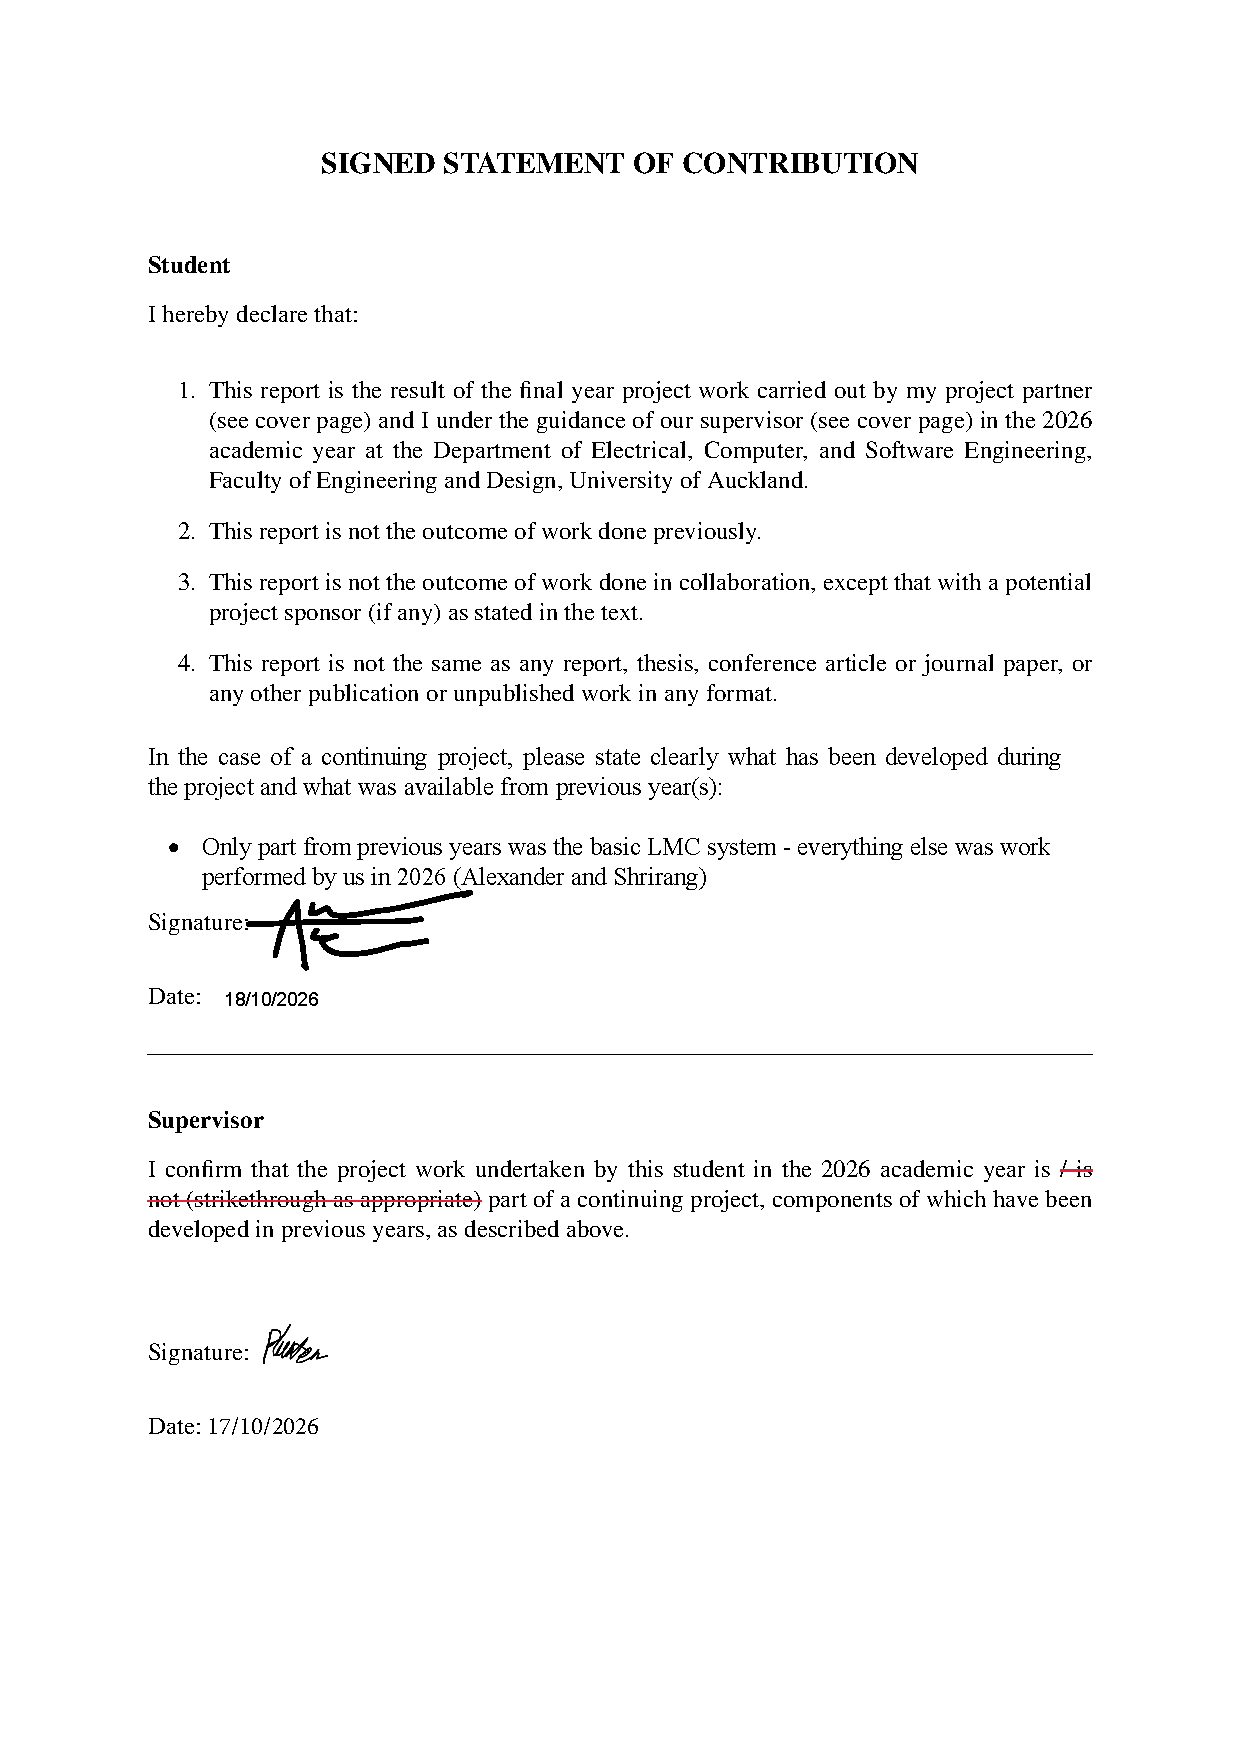
\includepdf[pagecommand=\thispagestyle{front}]{frontmatter/Declaration PAT SIGNED}
% \tableofcontents
% \listoffigures
% \listoftables
% \input{frontmatter/acknowledgements}
% \input{frontmatter/glossary}
% \input{frontmatter/abbreviations}
% \input{frontmatter/nomenclature}
% \printnomenclature
% \ifreview
%   \listoftodos[Review Notes]
% \fi

\clearpage{\pagestyle{empty}\cleardoublepage}% blank verso (if any) without a page number
\mainmatter
\bodyheadings
\bodyplainstyle
\pagestyle{lawton}
\include{chapters/01_Introduction}
\include{chapters/02_literature_review}
\include{chapters/03_experimental_design}
\include{chapters/04_Results}
\include{chapters/05_discussion_thermal}
\include{chapters/06_conclusion}

%\backmatter
%\printbibliography[heading=bibintoc,title={References}]

%\appendix
% cleveref does not detect \appendix here, so appendix chapters were cited as
% "Chapter A". Label them (and their sections) as appendices explicitly; the
% names are set with the other \crefname commands in the preamble.
%\crefalias{chapter}{appendix}
%\crefalias{section}{subappendix}
%\input{chapters/appendix/appendix_simscale_validation}
%\input{chapters/appendix/appendix_thermal_models}
%\input{chapters/appendix/appendix_femm_pump}

\end{document}
"
% =====================================================================
\documentclass[11pt,a4paper,twoside,openany]{report}

% The report class has no \frontmatter, \mainmatter or \backmatter (the book
% class does). Define them as in book.cls for the roman/arabic page numbering:
% with openany they start a new page, with openright a new odd page.
\makeatletter
\providecommand{\frontmatter}{%
  \if@openright\cleardoublepage\else\clearpage\fi\pagenumbering{roman}}
\providecommand{\mainmatter}{%
  \if@openright\cleardoublepage\else\clearpage\fi\pagenumbering{arabic}}
\providecommand{\backmatter}{%
  \if@openright\cleardoublepage\else\clearpage\fi}
\makeatother

\newif\ifreview
\reviewfalse
\ifdefined\REVIEW \reviewtrue \fi

% ---------------------------------------------------------------------
%  Fonts, language and page geometry
% ---------------------------------------------------------------------
\usepackage[T1]{fontenc}
\usepackage[utf8]{inputenc}
\usepackage{lmodern}                 % Computer Modern in T1 (as in Lawton)
\usepackage[british]{babel}          % NZ/UK spelling and hyphenation
\usepackage{microtype}
% Compact layout: narrow margins and near-single spacing, so that the body
% (Introduction to Conclusion) fits within 30 pages.
\usepackage[a4paper,top=20mm,bottom=20mm,inner=20mm,outer=20mm,
            headheight=14pt,headsep=6mm,footskip=10mm]{geometry}
\usepackage{setspace}
\setstretch{1.05}
\setlength{\emergencystretch}{1.5em}

% Display faces used for the title page and chapter openers
\newcommand{\chapnumfont}{\fontfamily{ppl}\fontseries{b}\selectfont}  % Palatino bold
\newcommand{\titlefont}{\fontfamily{bch}\fontseries{b}\selectfont}    % Charter bold

% ---------------------------------------------------------------------
%  Maths, units, tables, figures
% ---------------------------------------------------------------------
\usepackage{amsmath,amssymb}
\usepackage{siunitx}
\sisetup{
  per-mode            = symbol,
  inter-unit-product  = \ensuremath{\cdot},
  range-phrase        = --,
  range-units         = single,
  list-final-separator= {, and },
  product-units       = single,
}
\usepackage{graphicx}
\graphicspath{{figures/}}
\usepackage{booktabs,tabularx,array,multirow,makecell,longtable}
\renewcommand{\arraystretch}{1.15}
\newcolumntype{L}{>{\raggedright\arraybackslash}X}
\newcolumntype{C}{>{\centering\arraybackslash}X}
\usepackage{xcolor}
\definecolor{uoablue}{RGB}{0,70,127}
\usepackage{enumitem}
\setlist{itemsep=0pt,topsep=4pt}
\usepackage[labelsep=colon,skip=6pt]{caption}
\captionsetup[table]{position=top}
% All captions flush left, so short and long captions (and the notes below
% them) line up the same way.
\captionsetup{singlelinecheck=false}
% Captions are a short title only. Any further detail goes in a concise note:
% under the caption of a figure, or under the body of a table. \tnote marks
% the table cell that a note refers to.
\newcommand{\floatnote}[1]{\par\vspace{3pt}%
  {\raggedright\footnotesize\textit{Note:} #1\par}}
\newcommand{\tnote}[1]{\textsuperscript{#1}}
\usepackage{float}
\usepackage{placeins}                % \FloatBarrier keeps floats in their section
% Float placement. With LaTeX's defaults most floats here ended up on sparse
% float-only pages, centred vertically, away from the text that cites them.
% Allow more and larger floats on text pages (floats use [htbp]), accept a
% float-only page only when it is at least 3/4 full, and stack the floats at
% the top of such a page instead of spreading them down it.
\setcounter{topnumber}{3}
\setcounter{bottomnumber}{2}
\setcounter{totalnumber}{4}
\renewcommand{\topfraction}{0.85}
\renewcommand{\bottomfraction}{0.6}
\renewcommand{\textfraction}{0.12}
\renewcommand{\floatpagefraction}{0.75}
% When a page with floats cannot be filled exactly (e.g. the next heading does
% not fit), open up the gap between the floats and the text rather than the
% spacing between paragraphs.
\setlength{\textfloatsep}{14pt plus 12pt minus 4pt}
\setlength{\floatsep}{10pt plus 4pt minus 2pt}
\setlength{\intextsep}{10pt plus 4pt minus 2pt}
\makeatletter
\setlength{\@fptop}{0pt}
\setlength{\@fpsep}{\floatsep}
\setlength{\@fpbot}{0pt plus 1fil}
\makeatother
\usepackage{pdfpages}                % signed statement of contribution
\usepackage{nomencl}                 % nomenclature (ECSE template)
\makenomenclature
\usepackage[titles]{tocloft}         % TOC/LOF/LOT entries as in the ECSE template

\usepackage{subcaption}
% Subfigures: centred "(a) ..." captions, cited as "Fig. 4.5(a)"
\captionsetup[sub]{singlelinecheck=true,labelformat=simple}
\renewcommand{\thesubfigure}{(\alph{subfigure})}
\usepackage{pgfplots}
 \pgfplotsset{compat=1.17}
\usepgfplotslibrary{groupplots}      % multi-panel transient figures
\usepackage[american]{circuitikz}    % thermal network figure

% ---------------------------------------------------------------------
%  Headings
% ---------------------------------------------------------------------
\usepackage{titlesec}
% Chapter heading: bold Computer Modern, flush left, number and title on one
% line at the top of the page (compact layout).
\newcommand{\bodychapterformat}{%
  \titleformat{\chapter}[hang]
    {\normalfont\LARGE\bfseries\raggedright}
    {\thechapter}
    {0.8em}
    {}%
  \titleformat{name=\chapter,numberless}[hang]
    {\normalfont\LARGE\bfseries\raggedright}
    {}
    {0pt}
    {}%
  \titlespacing*{\chapter}{0pt}{0pt}{16pt}}
\bodychapterformat
\titleformat{\section}{\normalfont\large\bfseries}{\thesection}{1em}{}
\titleformat{\subsection}{\normalfont\normalsize\bfseries}{\thesubsection}{1em}{}
\titleformat{\subsubsection}{\normalfont\normalsize\bfseries}{\thesubsubsection}{1em}{}
\titlespacing*{\section}{0pt}{2.2ex plus .8ex minus .2ex}{1.0ex plus .2ex}
\titlespacing*{\subsection}{0pt}{1.8ex plus .6ex minus .2ex}{0.8ex plus .2ex}
\titlespacing*{\subsubsection}{0pt}{1.6ex plus .6ex minus .2ex}{0.5ex plus .2ex}
\setcounter{secnumdepth}{2}
\setcounter{tocdepth}{2}

% Front-matter headings follow the ECSE template (14 pt bold, flush left);
% \bodyheadings restores the body chapter heading for the main matter.
\newcommand{\frontheadings}{%
  \titleformat{name=\chapter,numberless}[block]
    {\normalfont\fontsize{14}{17}\selectfont\bfseries}{}{0pt}{}%
  \titlespacing*{\chapter}{0pt}{0pt}{12pt}}
\newcommand{\bodyheadings}{\bodychapterformat}

% ---------------------------------------------------------------------
%  ECSE template settings for the front matter
% ---------------------------------------------------------------------
\newcommand\HRule{\noindent\rule{\linewidth}{2pt}}   % title-page rules
\addto\captionsbritish{\renewcommand{\contentsname}{Table of Contents}}
% "Figure"/"Table" prefixes in the lists of figures and tables
\renewcommand{\cftfigpresnum}{Figure~}
\renewcommand{\cfttabpresnum}{Table~}
\setlength{\cftfignumwidth}{5.2em}
\setlength{\cfttabnumwidth}{5.2em}
% Nomenclature: "Symbols" / "Greek Symbols" groups with a unit column
\renewcommand{\nomname}{Nomenclature}
\def\nompreamble{\addcontentsline{toc}{chapter}{\nomname}\markboth{\nomname}{\nomname}}
\renewcommand{\nomgroup}[1]{%
  \ifthenelse{\equal{#1}{A}}{\item[\textbf{Symbols}]}{%
  \ifthenelse{\equal{#1}{G}}{\item[\textbf{Greek Symbols}]}{}}}
\newcommand{\nomunit}[1]{\renewcommand{\nomentryend}{\hspace*{\fill}#1}}
\setlength{\nomlabelwidth}{2.6cm}
\usepackage{ifthen}

% ---------------------------------------------------------------------
%  Running heads (Lawton: bold, ruled; page number outside;
%  chapter title on even pages, section on odd pages)
% ---------------------------------------------------------------------
\usepackage{fancyhdr}
\renewcommand{\chaptermark}[1]{\markboth{#1}{#1}}
\renewcommand{\sectionmark}[1]{\markright{\thesection\ \ #1}}
\fancypagestyle{lawton}{%
  \fancyhf{}%
  \fancyhead[LE]{\bfseries\thepage}%
  \fancyhead[RE]{\bfseries\nouppercase{\leftmark}}%
  \fancyhead[LO]{\bfseries\nouppercase{\rightmark}}%
  \fancyhead[RO]{\bfseries\thepage}%
  \renewcommand{\headrulewidth}{0.4pt}}
\pagestyle{lawton}
% Chapter opening pages use the plain style; in the body, give them the same
% ruled running head as every other page.
\newcommand{\bodyplainstyle}{%
  \fancypagestyle{plain}{%
    \fancyhf{}%
    \fancyhead[LE]{\bfseries\thepage}%
    \fancyhead[RE]{\bfseries\nouppercase{\leftmark}}%
    \fancyhead[LO]{\bfseries\nouppercase{\rightmark}}%
    \fancyhead[RO]{\bfseries\thepage}%
    \renewcommand{\headrulewidth}{0.4pt}}}
% ECSE template: no header, small centred page number
\fancypagestyle{front}{%
  \fancyhf{}%
  \fancyfoot[C]{\footnotesize\thepage}%
  \renewcommand{\headrulewidth}{0pt}}
\newcommand{\frontplainstyle}{%
  \fancypagestyle{plain}{%
    \fancyhf{}%
    \fancyfoot[C]{\footnotesize\thepage}%
    \renewcommand{\headrulewidth}{0pt}}}

% ---------------------------------------------------------------------
%  References (IEEE, with DOIs as in Lawton; source: Zotero export)
% ---------------------------------------------------------------------
\usepackage{csquotes}
\usepackage[backend=biber,style=ieee,
            doi=true,url=true,isbn=false,dashed=false,maxnames=6,minnames=1]{biblatex}
\addbibresource{zotero_references.bib}
\AtEveryBibitem{\clearfield{issn}%
  % an access date means nothing without a URL (e.g. Zotero items with no link)
  \iffieldundef{url}{\clearfield{urlyear}\clearfield{urlmonth}\clearfield{urlday}}{}}
% zotero_references.bib is the Zotero export; tidy its fields here rather than
% editing the file, so the fixes survive a refresh from Zotero. Drop language
% tags, ISBNs and the "ISSN: ..." notes Zotero writes, and give items that have
% a DOI only the DOI (no URL or access date).
\DeclareSourcemap{
  \maps[datatype=bibtex]{
    \map{
      \step[fieldset=language, null]
      \step[fieldset=isbn, null]
      \step[fieldsource=note, match=\regexp{\AISSN:}, final]
      \step[fieldset=note, null]
    }
    \map{
      \step[fieldsource=doi, final]
      \step[fieldset=url, null]
      \step[fieldset=urldate, null]
    }
    % Zotero stores an article number (e.g. 100133) as the page range; print it
    % as "Art. no." rather than as a page number
    \map{
      \pertype{article}
      \step[fieldsource=pages, notmatch=\regexp{-}, final]
      \step[fieldset=eid, origfieldval]
      \step[fieldset=pages, null]
    }
  }
}
\DeclareFieldFormat[article]{eid}{Art\adddot\space no\adddot\space#1}
% Some Zotero titles carry a zero-width space (U+200B), which pdfLaTeX cannot
% typeset; drop it here so the fix survives a refresh from Zotero. Also allow a
% line break after a Unicode em dash (U+2014), so that long titles such as
% Ouyang's do not run into the margin.
\DeclareUnicodeCharacter{200B}{}
\DeclareUnicodeCharacter{2014}{\textemdash\allowbreak}
% Break long DOIs and URLs without stretching the gaps around "." and "/"
\setcounter{biburlnumpenalty}{9000}
\setcounter{biburlucpenalty}{9000}
\setcounter{biburllcpenalty}{9000}
\biburlbigskip=0mu plus 1mu\relax

% ---------------------------------------------------------------------
%  Cross-referencing
% ---------------------------------------------------------------------
\usepackage[hidelinks,bookmarksnumbered]{hyperref}
\usepackage[nameinlink]{cleveref}
\crefname{chapter}{Chapter}{Chapters}
\crefname{section}{Section}{Sections}
\crefname{subsection}{Section}{Sections}
\crefname{figure}{Fig.}{Figs.}
\Crefname{figure}{Figure}{Figures}
\crefname{table}{Table}{Tables}
\crefname{appendix}{Appendix}{Appendices}
\crefname{subappendix}{Appendix}{Appendices}
\crefname{equation}{}{}
\crefformat{equation}{(#2#1#3)}
\crefrangeformat{equation}{(#3#1#4)--(#5#2#6)}
\crefmultiformat{equation}{(#2#1#3)}{ and~(#2#1#3)}{, (#2#1#3)}{ and~(#2#1#3)}

% ---------------------------------------------------------------------
%  Review notes
% ---------------------------------------------------------------------
\ifreview
  \usepackage[colorinlistoftodos,textsize=small]{todonotes}
    \newcommand{\issue}[1]{\par\todo[inline,color=orange!20,bordercolor=orange!70!black,
      linecolor=orange!70!black,caption={\textsc{Issue}: #1}]{\textbf{Issue:} #1}}
  \newcommand{\edited}[1]{\par\todo[inline,color=cyan!12,bordercolor=cyan!50!black,
      linecolor=cyan!50!black,caption={\textsc{Edited}: #1}]{\textbf{Edited:} #1}}
\else
  \newcommand{\issue}[1]{\ignorespaces}
  \newcommand{\edited}[1]{\ignorespaces}
\fi
% A value or detail still to be supplied. Always shown, in red, so that it
% cannot be missed in a submitted copy.
\newcommand{\missing}[1]{\textcolor{red}{[#1]}}
% \figureorplaceholder[options]{file}: as \includegraphics, but while
% figures/<file> does not exist yet it draws a framed placeholder naming the
% file, so the report still compiles.
\newcommand{\figureorplaceholder}[2][]{%
  \IfFileExists{figures/#2}{\includegraphics[#1]{#2}}{%
    \fbox{\parbox[c][4cm][c]{0.85\linewidth}{\centering
      \missing{Figure to be added: figures/\detokenize{#2}}}}}}

% ---------------------------------------------------------------------
%  Convenience macros
% ---------------------------------------------------------------------
\newcommand{\Vdot}{\dot{V}}
\newcommand{\mdot}{\dot{m}}
\newcommand{\cp}{c_{\mathrm{p}}}
\newcommand{\NTU}{\mathrm{NTU}}
\newcommand{\Rcp}{R_{\mathrm{cp}}}
\newcommand{\Rpack}{R_{\mathrm{pack}}}
\newcommand{\Rmisc}{R_{\mathrm{misc}}}
\newcommand{\Qin}{Q_{\mathrm{in}}}
\newcommand{\Qplate}{Q_{\mathrm{plate}}}
\newcommand{\Tin}{T_{\mathrm{in}}}
\newcommand{\Tout}{T_{\mathrm{out}}}
\newcommand{\Tres}{T_{\mathrm{resistor}}}
\newcommand{\Galinstan}{Galinstan}
\newcommand{\GaInSn}[3]{Ga\textsubscript{#1}In\textsubscript{#2}Sn\textsubscript{#3}}

% ---------------------------------------------------------------------
%  Report details (edit here)
% ---------------------------------------------------------------------
\newcommand{\reporttitle}{Liquid Metal Cooling for High-Power-Density Power Electronic Converters}
\newcommand{\reportauthor}{Alex Skilton}
\newcommand{\reporttype}{Final Report}
\newcommand{\reportdate}{\number\day\ \ifcase\month\or January\or February\or March\or April\or May\or June\or July\or August\or September\or October\or November\or December\fi\ \number\year}
\newcommand{\reportpartner}{Shrirang Ekbote}
\newcommand{\reportsupervisor}{Dr. Patrick Lawton and Prof. Grant Covic}

\hypersetup{pdftitle={\reporttitle},pdfauthor={\reportauthor}}

% =====================================================================
\begin{document}

\frontmatter
\frontheadings
\frontplainstyle
\pagestyle{empty}
%% =====================================================================
%  Title page -- 2026 ECSE Part IV Final Report template
%  (layout, rules, sizes and logo as in mainDocument.tex of the template;
%  type sizes are fixed at the template's 12 pt values)
% =====================================================================
\begin{titlepage}
\newgeometry{top=2cm,bottom=2cm,left=2.5cm,right=2.5cm}
\begin{spacing}{1}
\fontsize{12}{14.5}\selectfont
\setlength{\parindent}{0pt}
\setlength{\parskip}{\medskipamount}

\vspace*{10mm}

\begin{center}
\textbf{\fontsize{14.4}{18}\selectfont Research Project Report}
\end{center}

\vspace*{10mm}

\HRule
\begin{center}
\reporttype
\end{center}

\begin{center}
\textbf{\fontsize{17.28}{22}\selectfont \reporttitle}
\end{center}

\begin{center}
{\fontsize{14.4}{18}\selectfont \reportauthor}
\end{center}

\HRule

\vspace*{\fill}

\begin{center}
\begin{tabular}{rl}
Partner:  & \reportpartner \\
\noalign{\vskip1.5em}
Supervisor: & \reportsupervisor \\
\noalign{\vskip1.5em}
\end{tabular}
\end{center}

\vspace*{\fill}

\begin{center}
\reportdate
\end{center}

\vspace*{\fill}

\begin{center}

\includegraphics[width=0.7\linewidth]{UoA-Logo-Primary-RGB-Large}
\end{center}

\end{spacing}
\restoregeometry
\end{titlepage}


\pagestyle{front}
%% =====================================================================
%  Abstract page -- ECSE template layout
% =====================================================================
\thispagestyle{front}
\begingroup
\setlength{\parindent}{0pt}
\setlength{\parskip}{9pt}

\vspace*{1em}

\begin{center}
\textbf{\large \MakeUppercase{\reporttitle}}
\end{center}

\vspace{2em}

\begin{center}
\textbf{\large \reportauthor}
\end{center}

\vspace{2em}

\begin{center}
\textbf{\large ABSTRACT}
\end{center}

% Write your abstract here
[Abstract to be written.]
% end of Abstract

\endgroup
\clearpage


% Signed Statement of Contribution (student + supervisor). Replace
% frontmatter/Declaration.pdf with the signed copy.
% 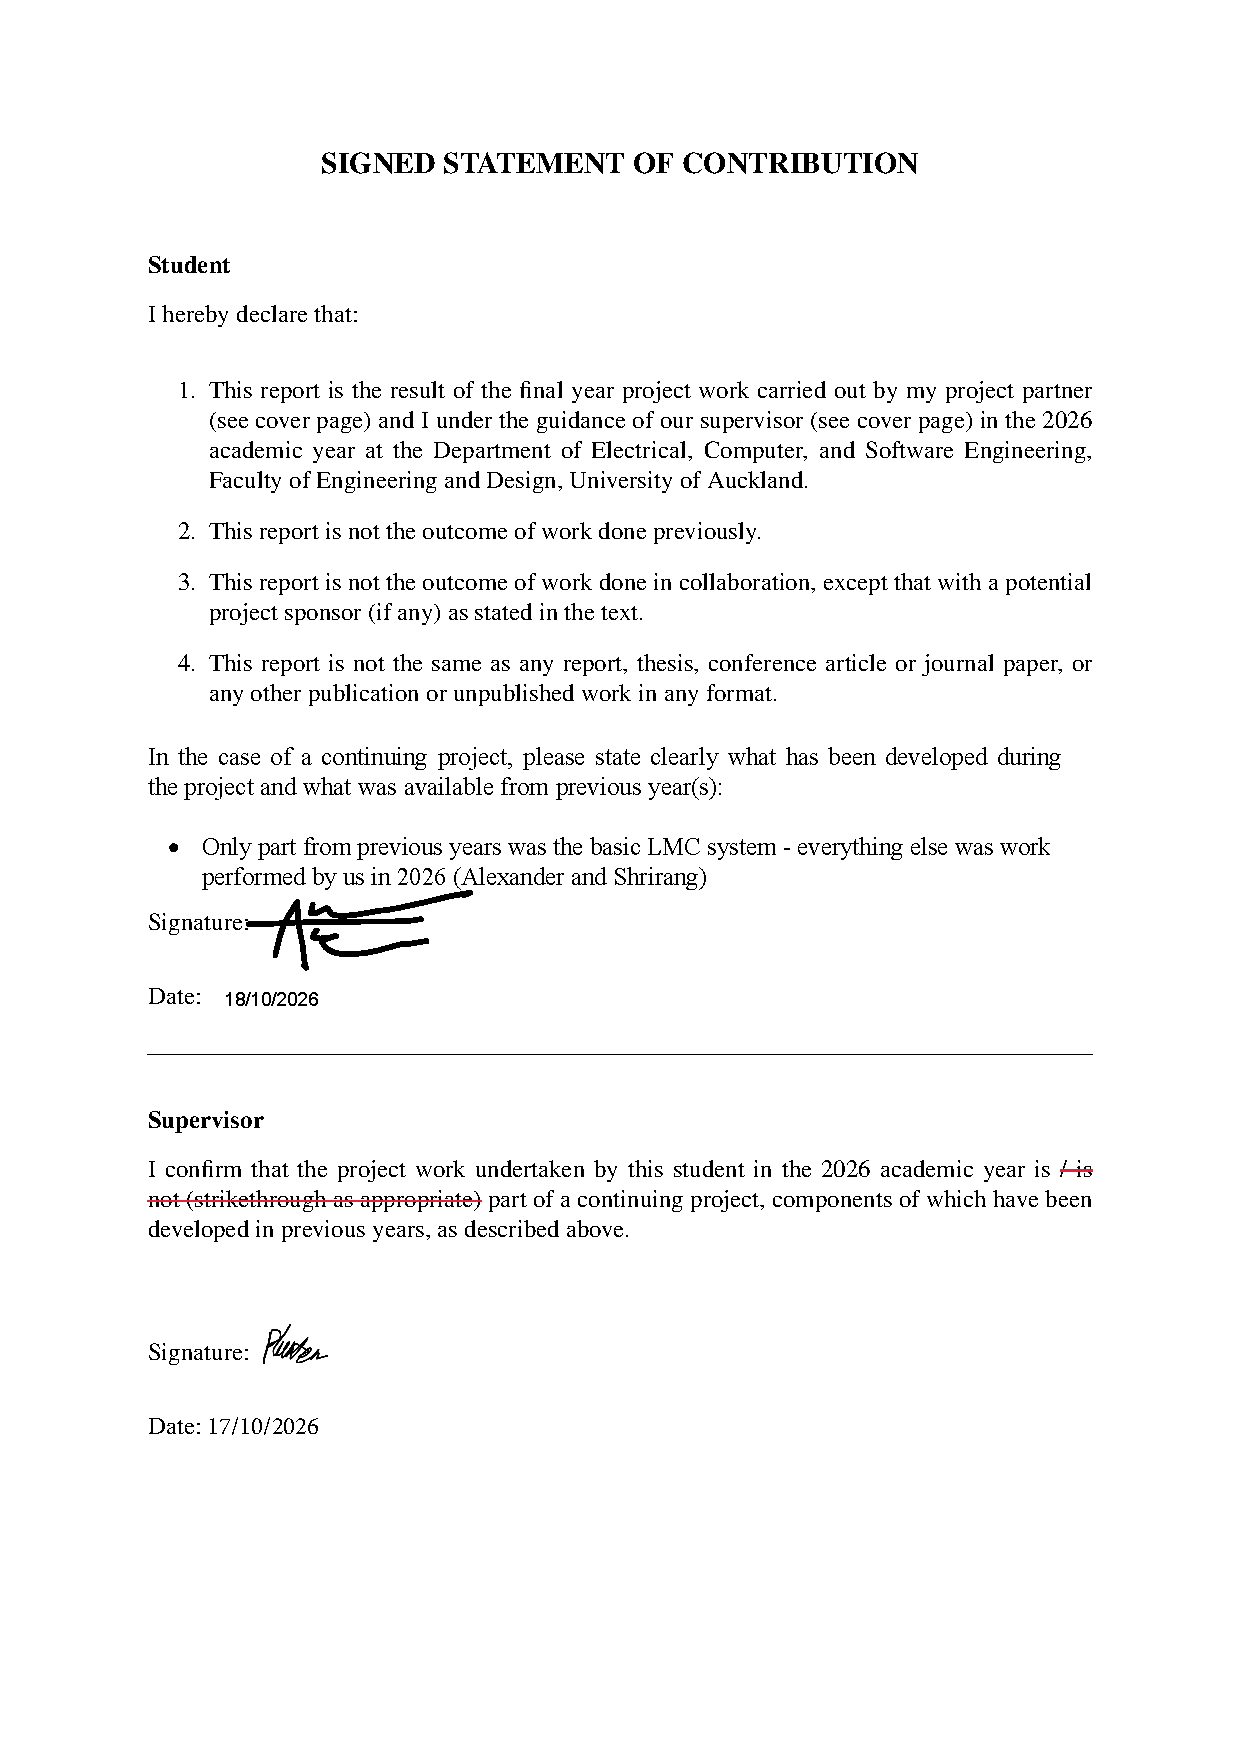
\includepdf[pagecommand=\thispagestyle{front}]{frontmatter/Declaration PAT SIGNED}
% \tableofcontents
% \listoffigures
% \listoftables
% % =====================================================================
%  Acknowledgements -- ECSE template
% =====================================================================
\chapter*{Acknowledgements}
\addcontentsline{toc}{chapter}{Acknowledgements}
\begingroup
\setlength{\parindent}{0pt}
\setlength{\parskip}{9pt}

Firstly, I would like to acknowledge my parents for their consistent love and support throughout my studies.

I would also like to express my sincere appreciation to my friend and project partner, Shrirang Ekbote, for his contributions, teamwork, and companionship throughout this project. It has been a long yet rewarding final year at university, and I look forward to continuing our journey together out in the professional world.

Thank you to my supervisors, Dr. Patrick Lawton and Professor Grant Covic, for their dedicated support, guidance, and expertise throughout this project. I truly appreciated your honest feedback and the time you took out of your busy schedules to encourage us when motivation was low. The lessons from this experience have undoubtedly made me a better engineer, and I will carry them with me into the future.

I would like to thank Cody Liu, Thor Bridger, Taha Basar, Howard Lu and the rest of the ECSE Power Electronics Lab for always being willing to help and contributing to a safe and functioning lab environment. 

Finally, thank you to all my other friends in the rest of the department and beyond, for contributing to the conversations, jokes, and memories throughout this year.

\endgroup

% % =====================================================================
%  Glossary of Terms -- ECSE template (Term / Definition longtable)
%  Definitions follow the usage in the report body; edit as needed.
% =====================================================================
\chapter*{Glossary of Terms}
\addcontentsline{toc}{chapter}{Glossary of Terms}

\begin{longtable}[l]{>{\raggedright}p{0.25\textwidth}>{\raggedright\arraybackslash}p{0.68\textwidth}}
\textbf{Term} & \textbf{Definition} \\
\addlinespace
Caloric resistance & Coolant temperature rise per unit heat load, $1/(\rho\,\cp\,\Vdot)$; the part of the thermal resistance set by the coolant's heat-capacity rate. \\
\addlinespace
Cold plate & Metal plate with internal coolant passages onto which heat-dissipating components are mounted. \\
\addlinespace
Conduction pump & Electromagnetic pump that drives a conductive liquid by passing a DC current through it across a magnetic field, producing a Lorentz force. \\
\addlinespace
Eddy current & Current induced in a conductor by a time-varying magnetic field, dissipating power as heat. \\
\addlinespace
Effectiveness & Ratio of the heat actually absorbed by the coolant to the maximum possible for the given inlet and wall temperatures. \\
\addlinespace
Galinstan & Eutectic gallium--indium--tin alloy that is liquid at room temperature. \\
\addlinespace
Power density & Power processed by a converter per unit volume. \\
\addlinespace
Skin depth & Depth at which an alternating current or field in a conductor has decayed to $1/e$ of its surface value. \\
\addlinespace
Thermal resistance & Temperature difference per unit heat flow between two points, in \si{\kelvin\per\watt}. \\
\end{longtable}
\addtocounter{table}{-1}

% % Abbreviations -- ECSE template layout (two-column longtable)
\chapter*{Abbreviations}
\addcontentsline{toc}{chapter}{Abbreviations}

\begin{longtable}[l]{>{\raggedright}p{0.25\textwidth}>{\raggedright\arraybackslash}p{0.68\textwidth}}
  AC    & Alternating current \\
  AI    & Artificial intelligence \\
  CAD   & Computer-aided design \\
  CHF   & Critical heat flux \\
  DC    & Direct current \\
  DCM   & Discontinuous conduction mode \\
  EM    & Electromagnetic \\
  EMF   & Electromotive force \\
  EV    & Electric vehicle \\
  Ga    & Gallium \\
  GaInSn & Gallium--indium--tin alloy (Galinstan) \\
  GaN   & Gallium nitride \\
  IPT   & Inductive power transfer \\
  LCC   & Inductor--capacitor--capacitor (compensation network) \\
  LCR   & Inductance--capacitance--resistance (meter) \\
  MHD   & Magnetohydrodynamic \\
  NaK   & Sodium--potassium alloy \\
  NTU   & Number of transfer units \\
  PEC   & Power electronic converter \\
  PFA   & Perfluoroalkoxy (polymer tubing) \\
  RQ    & Research question \\
  SiC   & Silicon carbide \\
  SMR   & Small modular reactor \\
  TIM   & Thermal interface material \\
  VA    & Volt-ampere \\
  ZVS   & Zero-voltage switching \\
\end{longtable}
\addtocounter{table}{-1}

% % Nomenclature (ECSE template: nomencl package, 'Symbols' and 'Greek Symbols'
% groups, unit in right-hand column). Prefix A = Symbols, G = Greek; the rest
% of the prefix is the sort key.

\nomenclature[Aa]{$A$}{Heat-transfer area of the cold-plate tube\nomunit{\si{\metre\squared}}}
\nomenclature[Ab]{$B$}{Magnetic flux density\nomunit{\si{\tesla}}}
\nomenclature[Actarget]{$C_{\mathrm{target}}$}{Target tuning capacitance\nomunit{\si{\farad}}}
\nomenclature[Acp]{$\cp$}{Specific heat capacity at constant pressure\nomunit{\si{\joule\per\kilogram\per\kelvin}}}
\nomenclature[Adh]{$D_{\mathrm{h}}$}{Hydraulic diameter\nomunit{\si{\metre}}}
\nomenclature[Ae]{$E$}{EMF measured by the flow sensor\nomunit{\si{\volt}}}
\nomenclature[Af]{$f$}{Frequency\nomunit{\si{\hertz}}}
\nomenclature[Ah]{$h$}{Convective heat transfer coefficient\nomunit{\si{\watt\per\metre\squared\per\kelvin}}}
\nomenclature[Ai1]{$I_{1}$}{Primary resonant current (rms)\nomunit{\si{\ampere}}}
\nomenclature[Ak]{$k$}{Thermal conductivity\nomunit{\si{\watt\per\metre\per\kelvin}}}
\nomenclature[Al]{$L$}{Heated tube length\nomunit{\si{\metre}}}
\nomenclature[Al1]{$L_{1}$}{Primary (inductor) self-inductance\nomunit{\si{\henry}}}
\nomenclature[Alg]{$l_{\mathrm{g}}$}{Air-gap length\nomunit{\si{\metre}}}
\nomenclature[Amdot]{$\mdot$}{Mass flow rate\nomunit{\si{\kilogram\per\second}}}
\nomenclature[An]{$N$}{Number of turns\nomunit{}}
\nomenclature[Anf]{$N_{\mathrm{f}}$}{Number of power cycles to failure\nomunit{cycles}}
\nomenclature[Anu]{Nu}{Nusselt number\nomunit{}}
\nomenclature[Antu]{NTU}{Number of transfer units, $hA/(\mdot\,\cp)$\nomunit{}}
\nomenclature[Ap]{$P$}{Tube perimeter\nomunit{\si{\metre}}}
\nomenclature[Aqqin]{$Q$, $\Qin$}{Heat load; input heat\nomunit{\si{\watt}}}
\nomenclature[Aqplate]{$\Qplate$}{Heat transferred into the cold plate\nomunit{\si{\watt}}}
\nomenclature[Arac]{$R_{\mathrm{ac}}$}{AC winding resistance\nomunit{\si{\ohm}}}
\nomenclature[Arcp]{$\Rcp$}{Cold-plate thermal resistance\nomunit{\si{\kelvin\per\watt}}}
\nomenclature[Armisc]{$\Rmisc$}{Thermal resistance to ambient\nomunit{\si{\kelvin\per\watt}}}
\nomenclature[Arpack]{$\Rpack$}{Package (resistor and interface) thermal resistance\nomunit{\si{\kelvin\per\watt}}}
\nomenclature[Are]{Re}{Reynolds number\nomunit{}}
\nomenclature[Ata]{$T_{\mathrm{A}}$}{Ambient temperature\nomunit{\si{\celsius}}}
\nomenclature[Atfx]{$T_{\mathrm{f}}(x)$}{Local coolant temperature\nomunit{\si{\celsius}}}
\nomenclature[Atintout]{$\Tin$, $\Tout$}{Coolant inlet and outlet temperatures\nomunit{\si{\celsius}}}
\nomenclature[Atj]{$T_{\mathrm{j}}$}{Junction temperature\nomunit{\si{\celsius}}}
\nomenclature[Atm]{$T_{\mathrm{M}}$}{Resistor (heat-source) node temperature\nomunit{\si{\celsius}}}
\nomenclature[Atp]{$T_{\mathrm{P}}$}{Isothermal plate node temperature\nomunit{\si{\celsius}}}
\nomenclature[Avdc]{$V_{\mathrm{DC}}$}{DC bus voltage\nomunit{\si{\volt}}}
\nomenclature[Avdot]{$\Vdot$}{Volumetric flow rate\nomunit{\si{\metre\cubed\per\second}}}
\nomenclature[Axres]{$X_{\mathrm{res}}$}{Resonant reactance\nomunit{\si{\ohm}}}
\nomenclature[Galphabeta]{$\alpha$, $\beta$}{Coffin--Manson fitting parameters\nomunit{}}
\nomenclature[Gdelta]{$\delta$}{Skin depth\nomunit{\si{\metre}}}
\nomenclature[Gdeltat]{$\Delta T$}{Temperature rise or swing\nomunit{\si{\kelvin}}}
\nomenclature[Gvarepsilon]{$\varepsilon$}{Cold-plate effectiveness\nomunit{}}
\nomenclature[Gmu]{$\mu$}{Dynamic viscosity\nomunit{\si{\pascal\second}}}
\nomenclature[Gmu0]{$\mu_{0}$}{Permeability of free space\nomunit{\si{\henry\per\metre}}}
\nomenclature[Grho]{$\rho$}{Density\nomunit{\si{\kilogram\per\metre\cubed}}}
\nomenclature[Gsigma]{$\sigma$}{Electrical conductivity\nomunit{\si{\siemens\per\metre}}}

% \printnomenclature
% \ifreview
%   \listoftodos[Review Notes]
% \fi

\clearpage{\pagestyle{empty}\cleardoublepage}% blank verso (if any) without a page number
\mainmatter
\bodyheadings
\bodyplainstyle
\pagestyle{lawton}
% =====================================================================
%  Chapter 1 -- Introduction (limited to one page)
% =====================================================================
\chapter{Introduction}
\label{ch:Introduction}

The continued electrification of the global economy is driving a sustained
increase in electricity demand~\cite{international_energy_agency_electricity_2025}.
Power electronic converters (PECs) enable this shift by electrifying
transport~\cite{bosshard_multi-objective_2016} and energy
systems~\cite{steimer_enabled_2010}. The power density of PECs has risen for decades,
driven by cost, functionality and hard weight and space
limits~\cite{steimer_enabled_2010,biela_cooling_2007}, and is projected to keep
rising~\cite{morroni_understanding_2023}. As converters shrink, however, the
same losses must be removed from a smaller volume, so thermal management
increasingly limits how far power density can
rise~\cite{biela_cooling_2007,morroni_understanding_2023}.

Inductive power transfer (IPT) chargers for electric vehicles illustrate this
challenge. At the standard \SI{85}{\kilo\hertz}~\cite{society_of_automotive_engineers_r_2024},
a \SI{10}{\kilo\watt} system dissipates several hundred watts, much of it in pads
that generate strong alternating magnetic fields~\cite{kim_thermal_2022}. Many
commercial designs already actively cool the coils~\cite{lawton_power_2024}, and
Liu \emph{et al.}\ call for new technologies to cool wireless
chargers~\cite{liu_thermal_2025}. Water cooling, however, is limited by the low
thermal conductivity of water~\cite{laloya_heat_2016}. Galinstan, a liquid metal
with much higher thermal conductivity~\cite{noauthor_gainsn_nodate}, can instead
be driven by a magnetohydrodynamic (MHD) pump with no moving
parts~\cite{hodes_potential_2014}, but its low volumetric heat capacity and
electrical conductivity bring trade-offs~\cite{hodes_potential_2014,an_liquid_2024}.
The extent of its advantage therefore remains unclear, as few studies compare it
with water at converter scale~\cite{fan_ultra-efficient_2026}.

This project builds on the 2025 Part~IV Project~\#51, in which Kwon and Loh
built an MHD-pumped Galinstan cooling loop and recommended comparing it with
water cooling and testing it near magnetic
components~\cite{kwon_project_2025,loh_project_2025}. Its aim is to evaluate
MHD-pumped Galinstan as a coolant for high-power-density PECs, and to identify
where in an IPT system it is most useful. The objectives are to (i)~compare the
thermal resistance and pumping power of the Galinstan loop with those of a water
loop using the same cold plate~\cite{ekbote_project_2026}; (ii)~explain and
extend the measurements with thermal models and a conjugate heat transfer
simulation; and (iii)~use a power-dense \SI{85}{\kilo\hertz} inductor to
demonstrate Galinstan cooling of magnetics and measure the eddy-current loss
induced in the coolant. These objectives are framed as two research questions
in \cref{sec:research-questions}. \Cref{ch:literature} reviews the literature,
\cref{ch:experimental} describes the methodology, \cref{ch:results} presents
the results, \cref{sec:discussion} discusses them and \cref{ch:conclusion}
concludes the report.

% =====================================================================
%  Chapter 2 -- Literature Review   (source: Literature_Review_Draft_v9.docx)
% =====================================================================
\chapter{Literature Review}
\label{ch:literature}
\edited{Section 2.3 restructured under three requirements (reliability, form
factor, efficiency), each comparing single-phase and phase-change cooling and
their implications for magnetic components. \Cref{tab:cooling-strategies} is
regrouped to match, with an added row for loss in magnetics.}

This chapter reviews the literature on cooling power electronic converters
(PECs) with liquid metal. It opens with the sources of loss in inductive power
transfer (IPT) systems, the application that motivates this work
(\cref{sec:ipt-losses}). It then presents the current trend that the power
density of PECs is increasing (\cref{sec:motivation}), and the reliability,
form-factor and efficiency requirements that their thermal management must meet,
which point to liquid metal cooling as a potential solution
(\cref{sec:thermal-management}). \Cref{sec:liquid-metal} evaluates this
proposal, and \cref{sec:research-gap} identifies the research gap and states
the research questions of this project.
\edited{The draft pointed to ``Section 2.6'' for the research gap; there is no
Section 2.6 (the gap is \cref{sec:research-gap}). All section, figure, table and
equation references are now generated with \texttt{\textbackslash cref}, so they
will stay correct if the structure changes.}

% ---------------------------------------------------------------------
\section{Thermal Losses in Inductive Power Transfer Systems}
\label{sec:ipt-losses}

IPT systems transfer power across a large air gap between loosely coupled
coils, and their losses are spread across the power electronics, the
compensation network and the magnetic pads. \Cref{fig:kim-losses} shows the
loss distribution that Kim \emph{et al.}\ measured and simulated for a
\SI{10}{\kilo\watt} IPT system with double-D (DD) pads, operating at
\SI{85}{\kilo\hertz} at a worst-case ambient temperature of
\SI{50}{\celsius}~\cite{kim_thermal_2022}. Most of the loss occurs in the pads,
chiefly in the Litz wire and ferrite, with smaller shares in the compensation
capacitors and in the aluminium shielding sheet, in which the leakage field
induces eddy currents. The inverter and rectifier dissipate about
\SIrange{70}{80}{\watt} each.

\begin{figure}[htbp]
  \centering
  \begin{tikzpicture}
    \begin{axis}[
      xbar stacked,
      width=0.78\linewidth, height=5.6cm,
      bar width=8pt,
      xmin=0, xmax=300,
      xlabel={Power loss (\si{\watt})},
      symbolic y coords={Inverter,Rectifier,Transformer,Cpi,Lsi,Secondary,Primary},
      ytick=data,
      yticklabels={Inverter, Rectifier, Transformer, $C_{\mathrm{pi}}$,
        $L_{\mathrm{si}}$, Secondary pad, Primary pad},
      tick label style={font=\small},
      label style={font=\small},
      xmajorgrids=true, grid style={dashed, gray!30},
      axis x line*=bottom, axis y line*=left,
      enlarge y limits=0.1,
      legend style={at={(0.98,0.04)}, anchor=south east, font=\small,
        draw=none, fill=white, fill opacity=0.85, text opacity=1},
      legend cell align=left,
    ]
      \addplot[fill=blue!60, draw=none] coordinates
        {(0,Inverter) (0,Rectifier) (0,Transformer) (0,Cpi) (0,Lsi) (40,Secondary) (165,Primary)};
      \addplot[fill=red!70, draw=none] coordinates
        {(0,Inverter) (0,Rectifier) (0,Transformer) (0,Cpi) (0,Lsi) (10,Secondary) (68,Primary)};
      \addplot[fill=green!55!black, draw=none] coordinates
        {(0,Inverter) (0,Rectifier) (0,Transformer) (0,Cpi) (0,Lsi) (12,Secondary) (39,Primary)};
      \addplot[fill=cyan!70, draw=none] coordinates
        {(0,Inverter) (0,Rectifier) (0,Transformer) (0,Cpi) (0,Lsi) (5,Secondary) (17,Primary)};
      \addplot[fill=brown!70, draw=none] coordinates
        {(80,Inverter) (70,Rectifier) (34,Transformer) (8,Cpi) (11,Lsi) (0,Secondary) (0,Primary)};
      \legend{Litz wire, Ferrite, Capacitors, Aluminium, Other components}
    \end{axis}
  \end{tikzpicture}
  \caption{Power loss distribution across a \SI{10}{\kilo\watt},
    \SI{85}{\kilo\hertz} IPT system with DD pads at an ambient temperature of
    \SI{50}{\celsius}, recreated from Kim \emph{et al.}~\cite{kim_thermal_2022}
    (values read from the original figure). $L_{\mathrm{si}}$ and $C_{\mathrm{pi}}$
    are components of the compensation network.}
  \label{fig:kim-losses}
\end{figure}

These losses differ in density. The pad losses are spread over about
\SI{0.8}{\metre} by \SI{0.6}{\metre} inside a strong alternating magnetic field,
and the pad is cooled passively, reaching a simulated peak temperature of about
\SI{96}{\celsius}. Its components also change with temperature: the Litz wire
resistance rises by about \SI{0.4}{\percent} per degree and the ferrite loss
varies nonlinearly, so power loss and temperature cannot be considered
separately~\cite{kim_thermal_2022}. The semiconductor losses, by contrast, are
concentrated in small switching devices placed away from the coupler. Where an
alternative coolant could be used in an IPT system therefore depends on both the
heat flux and the magnetic field the cooling system is exposed to, a question this report
returns to in \cref{sec:disc-suitability}.

Wireless charging of light-duty electric vehicles is standardised at a nominal
operating frequency of \SI{85}{\kilo\hertz}~\cite{society_of_automotive_engineers_r_2024},
the frequency used by Kim \emph{et al.}~\cite{kim_thermal_2022} and by
high-power IPT systems for public transport~\cite{bosshard_multi-objective_2016}.
The magnetic components of these systems are driven at this frequency, so any
cooling hardware placed near them is exposed to leakage fields at this
frequency. For this reason,
the power-dense inductor used in this work (\cref{sec:inductor-design}) is
operated at \SI{85}{\kilo\hertz}.
\issue{The Zotero record for SAE J2954 (\texttt{society\_of\_automotive\_engineers\_r\_2024})
has typos in its title (``J2594'', ``Vechicles''), which will print in the
reference list. Fix them in Zotero and re-export the bib file.}

% ---------------------------------------------------------------------
\section{Power Density in Power Electronic Converters}
\label{sec:motivation}

PECs switch semiconductor devices at high frequency and use passive components,
chiefly inductors, transformers and capacitors, to store and release energy in
each switching cycle and to filter the resulting
waveforms~\cite{morroni_understanding_2023}. Magnetic components, frequently the
largest passive devices, are difficult to scale and often restrict the
achievable power
density~\cite{biela_cooling_2007,morroni_understanding_2023,sullivan_size_2016};
with heat sinks, they account for the largest portion of a power solution's
size~\cite{biela_cooling_2007,morroni_understanding_2023}. Higher switching
frequencies, now practical with wide-bandgap devices~\cite{gao_modeling_2022},
permit smaller passive components because less energy is stored per
cycle~\cite{morroni_understanding_2023}, but losses limit this gain.

Friedli \emph{et al.}\ demonstrated this trade-off with \SI{10}{\kilo\watt}
rectifiers built for switching frequencies from \SI{72}{\kilo\hertz} to
\SI{1}{\mega\hertz}~\cite{friedli_essence_2014}. As the frequency rose, the
boost inductor shrank, but the efficiency fell almost linearly from
\SI{97.3}{\percent} to \SI{93}{\percent} as the switching losses grew. With
forced-air cooling, the growing heat sink cancelled the gain, so the power
density peaked at \SI{6.5}{\kilo\watt\per\deci\metre\cubed} near
\SI{350}{\kilo\hertz}, and \SI{1}{\mega\hertz} could not be air-cooled at all.
Only with water cooling did the power density keep rising, to
\SI{14.1}{\kilo\watt\per\deci\metre\cubed} at
\SI{1}{\mega\hertz}~\cite{friedli_essence_2014}. The cooling method therefore
sets the achievable power density, and as shrinking components raise the heat
flux~\cite{morroni_understanding_2023}, further size reduction requires cooling
methods that transfer more heat per unit area~\cite{biela_cooling_2007}.

% ---------------------------------------------------------------------
\section{Thermal Management of Power Electronic Converters}
\label{sec:thermal-management}

The thermal management of a power-dense PEC must meet three requirements. It
must keep the converter reliable, fit within its form factor, and do so
efficiently, without adding significant loss to the converter, including in
nearby magnetic components. The following sections consider each requirement
in turn, comparing the two established families of cooling: single-phase
cooling with air or water, and phase-change cooling by boiling or heat pipes.
\Cref{tab:cooling-strategies} summarises how each meets these
requirements~\cite{liu_thermal_2025,rahman_emerging_2024,laloya_heat_2016,mudawar_assessment_2001}.

\begin{table}[htbp]
  \centering
  \caption[Thermal management requirements and established cooling strategies]{Summary
    of how established cooling strategies meet the requirements for PEC thermal
    management. COP: coefficient of performance, the ratio of heat removed to
    cooling power consumed.}
  \label{tab:cooling-strategies}
  \small
  \begin{tabularx}{\linewidth}{@{}>{\raggedright\arraybackslash}p{3.0cm} L L@{}}
    \toprule
    Requirement & Single-phase (air, water) & Phase change (boiling, heat pipes) \\
    \midrule
    \multicolumn{3}{@{}l}{\textit{Reliability}} \\
    \quad Maximum temperature
      & Forced air: tens of \si{\watt\per\centi\metre\squared};
        water cold plate: hundreds of \si{\watt\per\centi\metre\squared};
        water microchannel: $\approx$\SI{1000}{\watt\per\centi\metre\squared}
      & Highest, but capped by CHF \\
    \quad Temperature swing
      & Fan speed or flow rate provides control input
      & Boiling-onset thermal shock; no control input when passive \\
    \addlinespace
    \multicolumn{3}{@{}l}{\textit{Form factor}} \\
    \quad Compactness
      & Air: bulky heat sink; water: compact at the device, pump and radiator remote
      & Smaller and lighter than single-phase \\
    \addlinespace
    \multicolumn{3}{@{}l}{\textit{Efficiency}} \\
    \quad Burden power
      & Fans (COP 10--100) or pump (COP 300--500); rises steeply as channels narrow
      & Low; often passive \\
    \quad Loss in magnetics
      & \multicolumn{2}{>{\raggedright\arraybackslash}p{0.62\linewidth}}{Any
        conductive cooling hardware in a leakage field incurs eddy-current loss} \\
    \bottomrule
  \end{tabularx}
\end{table}

\subsection{Reliability Requirement}
\label{sec:reliability}

Thermal management is required, above all, to keep increasingly power-dense
PECs reliable. Thermal stress causes over \SI{50}{\percent} of electronic
equipment failures~\cite{rahman_emerging_2024}, and power semiconductors, which
dominate the overall reliability of power converters, account for approximately
\SI{31}{\percent} of PEC failures~\cite{kalay_systematic_2025}. The
Coffin--Manson model relates the number of thermal cycles to failure of a
semiconductor device to its junction temperature
swing~\cite{kalay_systematic_2025,albarbar_thermal_2018}:
\begin{equation}
  N_{\mathrm{f}} = \alpha \left(\Delta T_{\mathrm{j}}\right)^{\beta},
  \label{eq:coffin-manson}
\end{equation}
where $N_{\mathrm{f}}$ is the number of power cycles (in thousands) to failure,
$\Delta T_{\mathrm{j}}$ is the junction temperature swing, and $\alpha$ and
$\beta$ are experimentally determined parameters~\cite{kalay_systematic_2025}.
This simplified form omits the absolute-temperature term, which becomes
significant mainly above about \SI{200}{\celsius}~\cite{kalay_systematic_2025}.
Magnetic components also fail under thermal
stress~\cite{biela_cooling_2007,mengesha_advanced_2025,li_review_2022,lawton_power_2024}.
For reliability, the cooling system must therefore hold the maximum temperature
of both semiconductors and magnetics below their operating limits, and suppress
the temperature swing.

Single-phase cooling meets both requirements to a degree. Natural convection,
the simplest scheme, is limited by the low heat transfer coefficient of
air~\cite{biela_cooling_2007}, and is the conventional way of cooling magnetic
components from their exposed surfaces. Gao \emph{et al.}'s passively cooled
planar inductor rose more than \SI{65}{\celsius} in temperature at
\SI{12}{\ampere} rms, whereas with an engineered conduction path to a
liquid-cooled cold plate (\cref{fig:gao-inductor}) the rise was less than
\SI{3}{\celsius}~\cite{gao_modeling_2022}. Forced air and liquid cooling raise
the achievable heat flux, and their fan speed or flow rate provides a control
input over the temperature swing. Their heat flux, however, is bounded by the
coolant~\cite{rahman_emerging_2024,laloya_heat_2016}. Phase-change cooling
absorbs latent heat and offers the highest heat
flux~\cite{laloya_heat_2016,mudawar_assessment_2001}. Above the critical heat
flux (CHF), however, vapour blocks liquid access to the surface and the device
temperature rises uncontrollably. CHF is difficult to predict, so the safety
margin it demands erodes this advantage~\cite{mudawar_assessment_2001}, and
passive phase-change schemes offer no control over the temperature swing.

\begin{figure}[tbp]
  \centering
  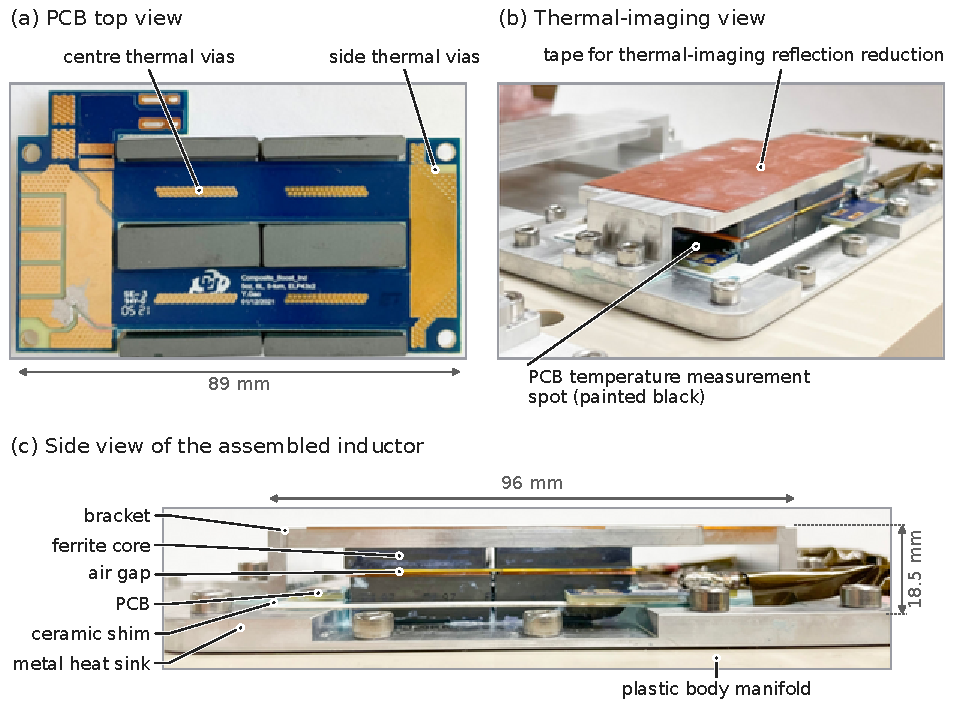
\includegraphics[width=0.75\linewidth]{gao_inductor_prototype}
  \caption[Planar inductor prototype of Gao \emph{et al.}]{Planar inductor
    prototype of Gao \emph{et al.} with an engineered conduction path to the
    cold plate: (a)~PCB top view; (b)~view used for thermal imaging;
    (c)~side view of the assembled inductor. Adapted
    from~\cite{gao_modeling_2022}.}
  \label{fig:gao-inductor}
\end{figure}

\subsection{Form Factor Requirement}
\label{sec:form-factor}

The cooling system must not erode the power density it is meant to enable. With
the magnetic components, heat sinks account for the largest portion of a power
converter's size, and in compact converters the thermal management system can
occupy a large share of the
volume~\cite{biela_cooling_2007,morroni_understanding_2023,friedli_essence_2014}.
Air cooling requires bulky heat sinks, which limited the power density of the
rectifiers of Friedli \emph{et al.}\ (\cref{sec:motivation}). Water cooling is
compact at the device, as the pump and radiator can be placed
remotely~\cite{friedli_essence_2014,laloya_heat_2016}, while phase-change
systems can be smaller and lighter still~\cite{laloya_heat_2016}. For magnetic
components, a compact cooling system must be placed as close as possible to the
windings, typically on both the top and bottom of the
core~\cite{krismer_accurate_2010,biela_cooling_2007}, which places it directly in
the component's leakage field.

\subsection{Efficiency Requirement}
\label{sec:efficiency-req}

To retain the efficiency of the converter, the power drawn by the cooling system,
its burden power, must remain small relative to the power
processed~\cite{laloya_heat_2016}, and the cooling hardware must not introduce
excessive loss into the converter. Single-phase cooling requires fans or pumps,
and raising its heat flux requires narrower channels, which raise the pressure
drop and pumping power steeply~\cite{rahman_emerging_2024,laloya_heat_2016}.
Single-phase cooling therefore trades the maximum temperature it can hold
against the burden power it draws. Phase-change cooling draws little or no
burden power, and is often passive~\cite{laloya_heat_2016}.

Cooling hardware placed near magnetic components, whether single-phase or
phase-change, sits in their leakage field and suffers eddy-current
loss~\cite{biela_cooling_2007,gao_modeling_2022,ouyang_overview_2014}. In Gao
\emph{et al.}'s design, the cold plate and bracket raised the measured AC winding
resistance by \SI{34}{\percent}~\cite{gao_modeling_2022}, and the aluminium
shielding sheet of an IPT pad dissipates about \SI{17}{\watt} in the same way
(\cref{fig:kim-losses})~\cite{kim_thermal_2022}. Biela and Kolar similarly found
that heat-transfer components near an inductor air gap must be recessed from
it~\cite{biela_cooling_2007}. Because magnetic components are present in most
converters~\cite{morroni_understanding_2023}, their leakage fields must be
considered in any PEC cooling design, even where the magnetics are not the main
thermal constraint.

No established scheme therefore meets all three requirements. Phase-change
cooling offers the highest heat flux at low burden power, but is capped by CHF
and offers no control over the temperature swing when passive. Single-phase
cooling is controllable, but its heat flux is bounded by the low thermal
conductivity of air and water, so a higher heat flux costs pumping power. A
coolant with substantially higher thermal conductivity could ease this trade-off
while keeping flow-rate control, which motivates much of the research into
liquid metal coolants~\cite{hodes_potential_2014}.

% ---------------------------------------------------------------------
\section{Liquid Metal as a Coolant}
\label{sec:liquid-metal}

Liquid metals have long been used as coolants where heat fluxes and operating
temperatures exceed those that conventional fluids can tolerate~\cite{rowinski_small_2015}. 
Much of the early characterisation of liquid metal cooling systems was carried out as fundamental research for nuclear
reactors~\cite{rowinski_small_2015}. These systems typically use lead or sodium
coolants, but lead is toxic and requires careful handling and
containment~\cite{oecd_handbook_2015}, whereas sodium is highly chemically
reactive, particularly with water and air, posing fire and explosion
hazards~\cite{foust_sodium-nak_1972}. These factors complicate broader commercial
deployment.

Liquid metal has more recently been proposed as a coolant for computing hardware and
PECs~\cite{fan_ultra-efficient_2026,zhang_water-based_2015}. The driving factor is its high thermal
conductivity, which promises high heat transfer rates~\cite{hodes_potential_2014,fan_ultra-efficient_2026,zhang_experimental_2019,zhang_investigation_2023}.
Such applications typically use gallium (Ga)-based eutectic alloys, the most
common being Galinstan (GaInSn), which is non-toxic and remains liquid at room temperature~\cite{hodes_potential_2014,an_liquid_2024}. 
Galinstan has a thermal conductivity of \SI{16.5}{\watt\per\metre\per\kelvin},
approximately 28 times that of water (\cref{tab:galinstan-properties}), which
enhances heat spreading and reduces temperature gradients~\cite{hodes_potential_2014,zhang_experimental_2019}. 
A Galinstan loop offers single-phase cooling, with no boiling limit to design around, and has the potential to
remove a higher heat flux than water~\cite{hodes_potential_2014, zhang_experimental_2019}.

These benefits come with significant trade-offs (\cref{tab:galinstan-properties}).
High density and viscosity raise pumping power and system weight. Because the
volumetric heat capacity is low, more than twice the flow of water is needed
for the same coolant temperature rise. Electrical conductivity rules out direct
contact with live parts and exposes the coolant to induction heating. 
The wide liquid range, by contrast, removes the CHF limit that
constrains phase-change cooling. The material cost is high, but at the
system level water and Galinstan are comparable because water pumps are
expensive~\cite{fan_ultra-efficient_2026}. Kwon~\cite{kwon_project_2025}
therefore concluded that liquid metal suits specialised applications where
efficiency, compactness and reliability justify its cost.

\begin{table}[htbp]
  \centering
  \caption{Selected properties and cost of the Galinstan used in this work
    (Rich Metals grade EU-10C, 68.5Ga--21.5In--10Sn by
    weight~\cite{noauthor_gainsn_nodate}) relative to water.}
  \label{tab:galinstan-properties}
  \small
  \begin{tabularx}{\linewidth}{@{}>{\raggedright\arraybackslash}p{3.2cm}
      >{\raggedright\arraybackslash}p{2.9cm} L >{\raggedright\arraybackslash}p{1.3cm}@{}}
    \toprule
    Property & Galinstan & Relative to water & Source \\
    \midrule
    Thermal conductivity & \SI{16.5}{\watt\per\metre\per\kelvin} & About 28 times higher & \cite{noauthor_gainsn_nodate} \\
    Density & \SI{6370}{\kilogram\per\metre\cubed} & More than six times higher & \cite{noauthor_gainsn_nodate} \\
    Dynamic viscosity & \SI{2}{\milli\pascal\second} & About 2 times higher & \cite{noauthor_gainsn_nodate} \\
    Specific heat capacity & \SI{366}{\joule\per\kilogram\per\kelvin} & About one-fourteenth & \cite{zhang_experimental_2019} \\
    Volumetric heat capacity & \SI{2.3}{\mega\joule\per\metre\cubed\per\kelvin} & 0.45 times, so about 2.2 times the flow for equal $\Delta T$ & \cite{noauthor_gainsn_nodate} \\
    Electrical conductivity & \SI{3.46e6}{\siemens\per\metre} & Conductor (deionised water: \SI{5.5e-6}{\siemens\per\metre}) & \cite{noauthor_gainsn_nodate} \\
    Melting and boiling points & \SI{10}{\celsius} and above \SI{1300}{\celsius} & Liquid above \SI{10}{\celsius}, so it can solidify in cold storage; boiling will not occur & \cite{noauthor_gainsn_nodate,hodes_potential_2014} \\
    Material cost & US\$200--2000/kg & Orders of magnitude higher & \cite{an_liquid_2024} \\
    \bottomrule
  \end{tabularx}
\end{table}

Much of the reviewed work on Galinstan and other Ga-based coolants focuses on
micro- and mini-channel heat sinks for electronics, typically for heat loads
from watts to hundreds of watts. It is unclear from the literature whether such
systems can be scaled up to the channel sizes and temperatures more typical of
PECs. For example, EV-charging PECs have power classes on the order of tens of
kilowatts for light-duty vehicles and are being standardised up to
\SI{1}{\mega\watt} for heavy-duty
vehicles~\cite{lawton_power_2024,liu_thermal_2025,abb_e-mobility_mcs1200_nodate}. Large liquid
metal systems have been realised for nuclear reactors~\cite{rowinski_small_2015},
but these use different metals, operate at much higher temperatures and are much
larger than even the most powerful PEC applications, although some work has
addressed power electronic
converters~\cite{fan_ultra-efficient_2026,fan_liquid_2021}.

% ---------------------------------------------------------------------
\subsection{Electromagnetic Pumping}
\label{sec:em-pumping}

The low volumetric heat capacity of Galinstan makes pumping demanding. For a
heat load $Q$ and coolant temperature rise $\Delta T$, the required volumetric
flow rate is
\begin{equation}
  \Vdot = \frac{Q}{\rho \, \cp \, \Delta T},
  \label{eq:flow-requirement}
\end{equation}
where $\rho$ is the coolant density and $\cp$ its specific heat capacity.
Galinstan therefore needs about 2.2 times the flow of water
(\cref{tab:galinstan-properties}), which is identified as the primary
bottleneck for liquid metal heat sinks~\cite{hodes_potential_2014,an_liquid_2024}.
Its high thermal conductivity partly offsets this, because it sustains high heat
transfer coefficients in wider channels with a lower pressure
drop~\cite{zhang_water-based_2015,an_liquid_2024}.

The electrical conductivity of Galinstan also allows it to be driven by
electromagnetic (EM) pumps with no moving parts, which are silent,
vibration-free and compact~\cite{hodes_potential_2014}. Previous Part~IV
projects used a permanent-magnet DC conduction
pump~\cite{kwon_project_2025,loh_project_2025}. In this pump, a current $I$
passed through the coolant perpendicular to a magnetic field of flux density
$B$ produces a Lorentz force density
$\mathbf{J}\times\mathbf{B}$~\cite{kwon_project_2025}. An approximation for the
pressure developed is
\begin{equation}
  \Delta p = \frac{B I}{h},
  \label{eq:mhd-pressure}
\end{equation}
where $h$ is the channel height parallel to
$\mathbf{B}$~\cite{loh_project_2025}. Pressure therefore scales directly with
current, so the flow can be modulated to suppress temperature
swing~\cite{an_liquid_2024}, and shallow channels with strong magnets are
favoured. The cost is operation at high current and low voltage
(\SIrange{1}{100}{\ampere}, \SIrange{0.01}{0.5}{\volt},
\SIrange{0.1}{50}{\watt}), with efficiencies of only about
\SIrange{6}{10}{\percent}~\cite{an_liquid_2024,hodes_potential_2014}. Even
so, a conduction pump has drawn less than \SI{15}{\percent} of the power of a
mechanical water pump for the same cooling performance~\cite{an_liquid_2024}.

Induction pumps instead induce current in the coolant through an alternating or
travelling field. They are larger and more complex, but they develop greater
force~\cite{an_liquid_2024}. The field can also come from the converter itself.
Fan \emph{et al.}\ integrated an MHD pump into an inductor, so that the flow
self-adjusts with converter load~\cite{fan_liquid_2021}. The cost is
eddy-current losses in the coolant~\cite{fan_ultra-efficient_2026}. EM pumps
are, however, generally reported as individual designs. Among liquid metal
systems developed for power electronics, only those of Fan
\emph{et al.}\ have been compared against an equivalent water
system~\cite{fan_liquid_2021,fan_ultra-efficient_2026}.

% ---------------------------------------------------------------------
\subsection{Compatibility with Electrical Equipment}
\label{sec:compatibility}

Commercial use of Galinstan raises three concerns: material safety, corrosion
and electromagnetic compatibility. Galinstan was developed as a non-toxic,
non-flammable replacement for mercury. Its negligible vapour pressure means it
poses no inhalation risk~\cite{hodes_potential_2014}. Gallium oxide can damage
the respiratory system at high airborne concentrations, but a closed loop
releases only minimal amounts~\cite{an_liquid_2024}. Prior prototypes managed
skin contact and spillage with gloves, eye protection and containment
trays~\cite{kwon_project_2025,loh_project_2025}.

Ga-based alloys corrode aluminium severely, and copper requires protection
above \SI{100}{\celsius}~\cite{an_liquid_2024}. Erosion at high flow velocities
and the effect on ductile metals remain unstudied~\cite{hodes_potential_2014}.
Plastics and nickel-plated metals~\cite{hodes_potential_2014}, as well as
ceramics such as aluminium nitride~\cite{an_liquid_2024}, are compatible.
Aluminium nitride is also both thermally conductive and electrically
insulating, though expensive~\cite{gao_modeling_2022}.

Electrically, the coolant is a conductor. A leak onto
energised circuitry is a direct short~\cite{hodes_potential_2014}. The loop also
galvanically connects every wetted part, so the EM pump supply can energise the
radiator and cold plate~\cite{kwon_project_2025}. There is also potential for nearby
magnetics to induce eddy currents in the coolant, though this has not been strictly explored in the literature
(\cref{sec:thermal-management})~\cite{an_liquid_2024, fan_ultra-efficient_2026}.
As a result, low-cost plastic piping suits low-field regions. 
Near magnetics, it may be preferable to shield the coolant with a more conductive material to reduce eddy losses.

% ---------------------------------------------------------------------
\section{Research Gap and Objectives}
\label{sec:research-gap}

\subsection{Research Gap}
\edited{Trimmed only. The two opening sentences (water cooling is bounded by
water's thermal conductivity; Galinstan's higher conductivity can improve heat
transfer, both cited to Hodes \emph{et al.}) repeated
\cref{sec:thermal-management,sec:liquid-metal} and were cut. The two closing
sentences of the second gap (most converters contain magnetics; a cooling
system that does not cool them must still tolerate their leakage fields) are
now made in \cref{sec:thermal-management} and are replaced by a back-reference.
In the first gap, ``which use different metals at much higher temperatures''
was cut, as \cref{sec:liquid-metal} already says so.}

This study aims to address two gaps identified in the literature.

The first is the lack of comparisons between water and liquid metal at the scale
of a converter's cooling loop. Most existing comparisons are made for micro- and
mini-channel heat
sinks~\cite{hodes_potential_2014,zhang_water-based_2015,zhang_experimental_2019,an_liquid_2024},
or lie at the scale of nuclear reactors~\cite{rowinski_small_2015}. This study
aims to quantify the
trade-offs of the Galinstan system (as designed
in~\cite{kwon_project_2025,loh_project_2025}) relative to a comparable water-cooling
system.

The second is the cooling of magnetic components with Galinstan. To the author's
knowledge, no study has demonstrated Galinstan cooling of a magnetic component,
such as a power-dense inductor, or quantified the eddy-current losses induced in
the coolant by its leakage field. Eddy-current losses have been assessed in AC
conduction pumps~\cite{fan_ultra-efficient_2026}, and an inductor has been used to drive a
pump~\cite{fan_ultra-efficient_2026,fan_liquid_2021}, but not to cool the inductor itself
directly. As argued in \cref{sec:thermal-management}, the coolant's loss in a
leakage field matters even where the coolant does not cool the magnetics.

This project addresses both gaps using the existing Galinstan loop of
Loh~\cite{loh_project_2025} and Kwon~\cite{kwon_project_2025}. The loop comprises a
permanent-magnet MHD pump, perfluoroalkoxy (PFA) tubing, a cold plate and a
fan-cooled radiator, and can remove up to a \SI{72}{\watt} resistive
load~\cite{kwon_project_2025,loh_project_2025}. The loop was not tested against water
in the same apparatus, and its experiments did not consider magnetics:
Loh~\cite{loh_project_2025} focused on switching devices because Galinstan was
unlikely to interfere with them, unlike magnetics, and Kwon~\cite{kwon_project_2025}
excluded direct integration and testing with magnetics because of time
limitations and uncertainty about electromagnetic interference. Both recommended
comparison with water cooling, and Kwon also recommended testing higher heat
loads and investigating the interaction with inductive pad
fields~\cite{kwon_project_2025,loh_project_2025}.
\edited{``This project was not tested against water'' referred to the previous
project's loop, not this project; reworded to ``The loop was not tested
\dots''.}

\subsection{Research Questions}
\label{sec:research-questions}

These gaps lead to two research questions.

\begin{description}[leftmargin=3.2em,labelwidth=2.6em,labelsep=0.6em,itemsep=4pt]
    \item[RQ1] At the same heat load, how do the thermal resistance and pumping
    power of the Galinstan loop compare with those of a similar conventional
    water loop?
    \item[H1] Galinstan's higher thermal conductivity will lower the convective
    resistance relative to water in the same cold plate. However, the total
    thermal resistance of the Galinstan loop will be higher than that of the
    water loop. Its low volumetric heat capacity and low flow rate give a
    caloric resistance comparable to the conduction resistance of the cold
    plate.
    \item[RQ2] Can the Galinstan loop cool a power-dense inductor while adding
    minimal loss to the existing aluminium cold plate, and how large is the
    eddy-current loss induced in the coolant?
    \item[H2] The Galinstan loop will have a cooling effect on the inductor above that of natural convection. 
    The increase in loss due to eddy-current loss induced in the coolant will be
    small compared to the loss of introducing the cold plate.
    The metal of the cold plate between the inductor and the coolant is
    several skin depths thick at \SI{85}{\kilo\hertz}. Additionally, the high-frequency field will not change the coolant flow
    measurably. 
\end{description}

% =====================================================================
%  Chapter 3 -- Methodology
%  Structure follows the Experimental Section of Kwon (2025): setup,
%  design, modelling, then the experimental procedure.
% =====================================================================
\chapter{Methodology}
\label{ch:experimental}

The following sections detail the methodology used to evaluate
magnetohydrodynamically pumped Galinstan as a coolant for PECs. Two objectives
guided the work. The first is to compare the thermal performance of the
Galinstan cooling loop with that of a similar water cooling loop under
equivalent operating conditions (RQ1). The second is to quantify the influence
of a high-frequency magnetic leakage field on the Galinstan coolant (RQ2).
\Cref{sec:setup} describes the experimental setup, including the two cooling
loops, the instrumentation and the safety considerations.
\Cref{sec:inductor-design} presents the design of the power-dense inductor used
as the heat source in the second experiment. \Cref{sec:thermal-model} develops
the thermal models used to interpret the measurements, and
\cref{sec:programme} gives the procedures for the two experiments.

% ---------------------------------------------------------------------
\section{Experimental Setup}
\label{sec:setup}

\subsection{Cooling System Overview}
\label{sec:loop-overview}

Two cooling loops were used in this project, one circulating Galinstan and the
other water. Both follow the arrangement shown in \cref{fig:cooling-loop}. A
pump drives the coolant through a cold plate that interfaces with the heat
source, and then through a fan-cooled radiator, where the heat is rejected to
the environment. A flow sensor in the hot line measures the coolant flow rate.

\begin{figure}[htbp]
  \centering
  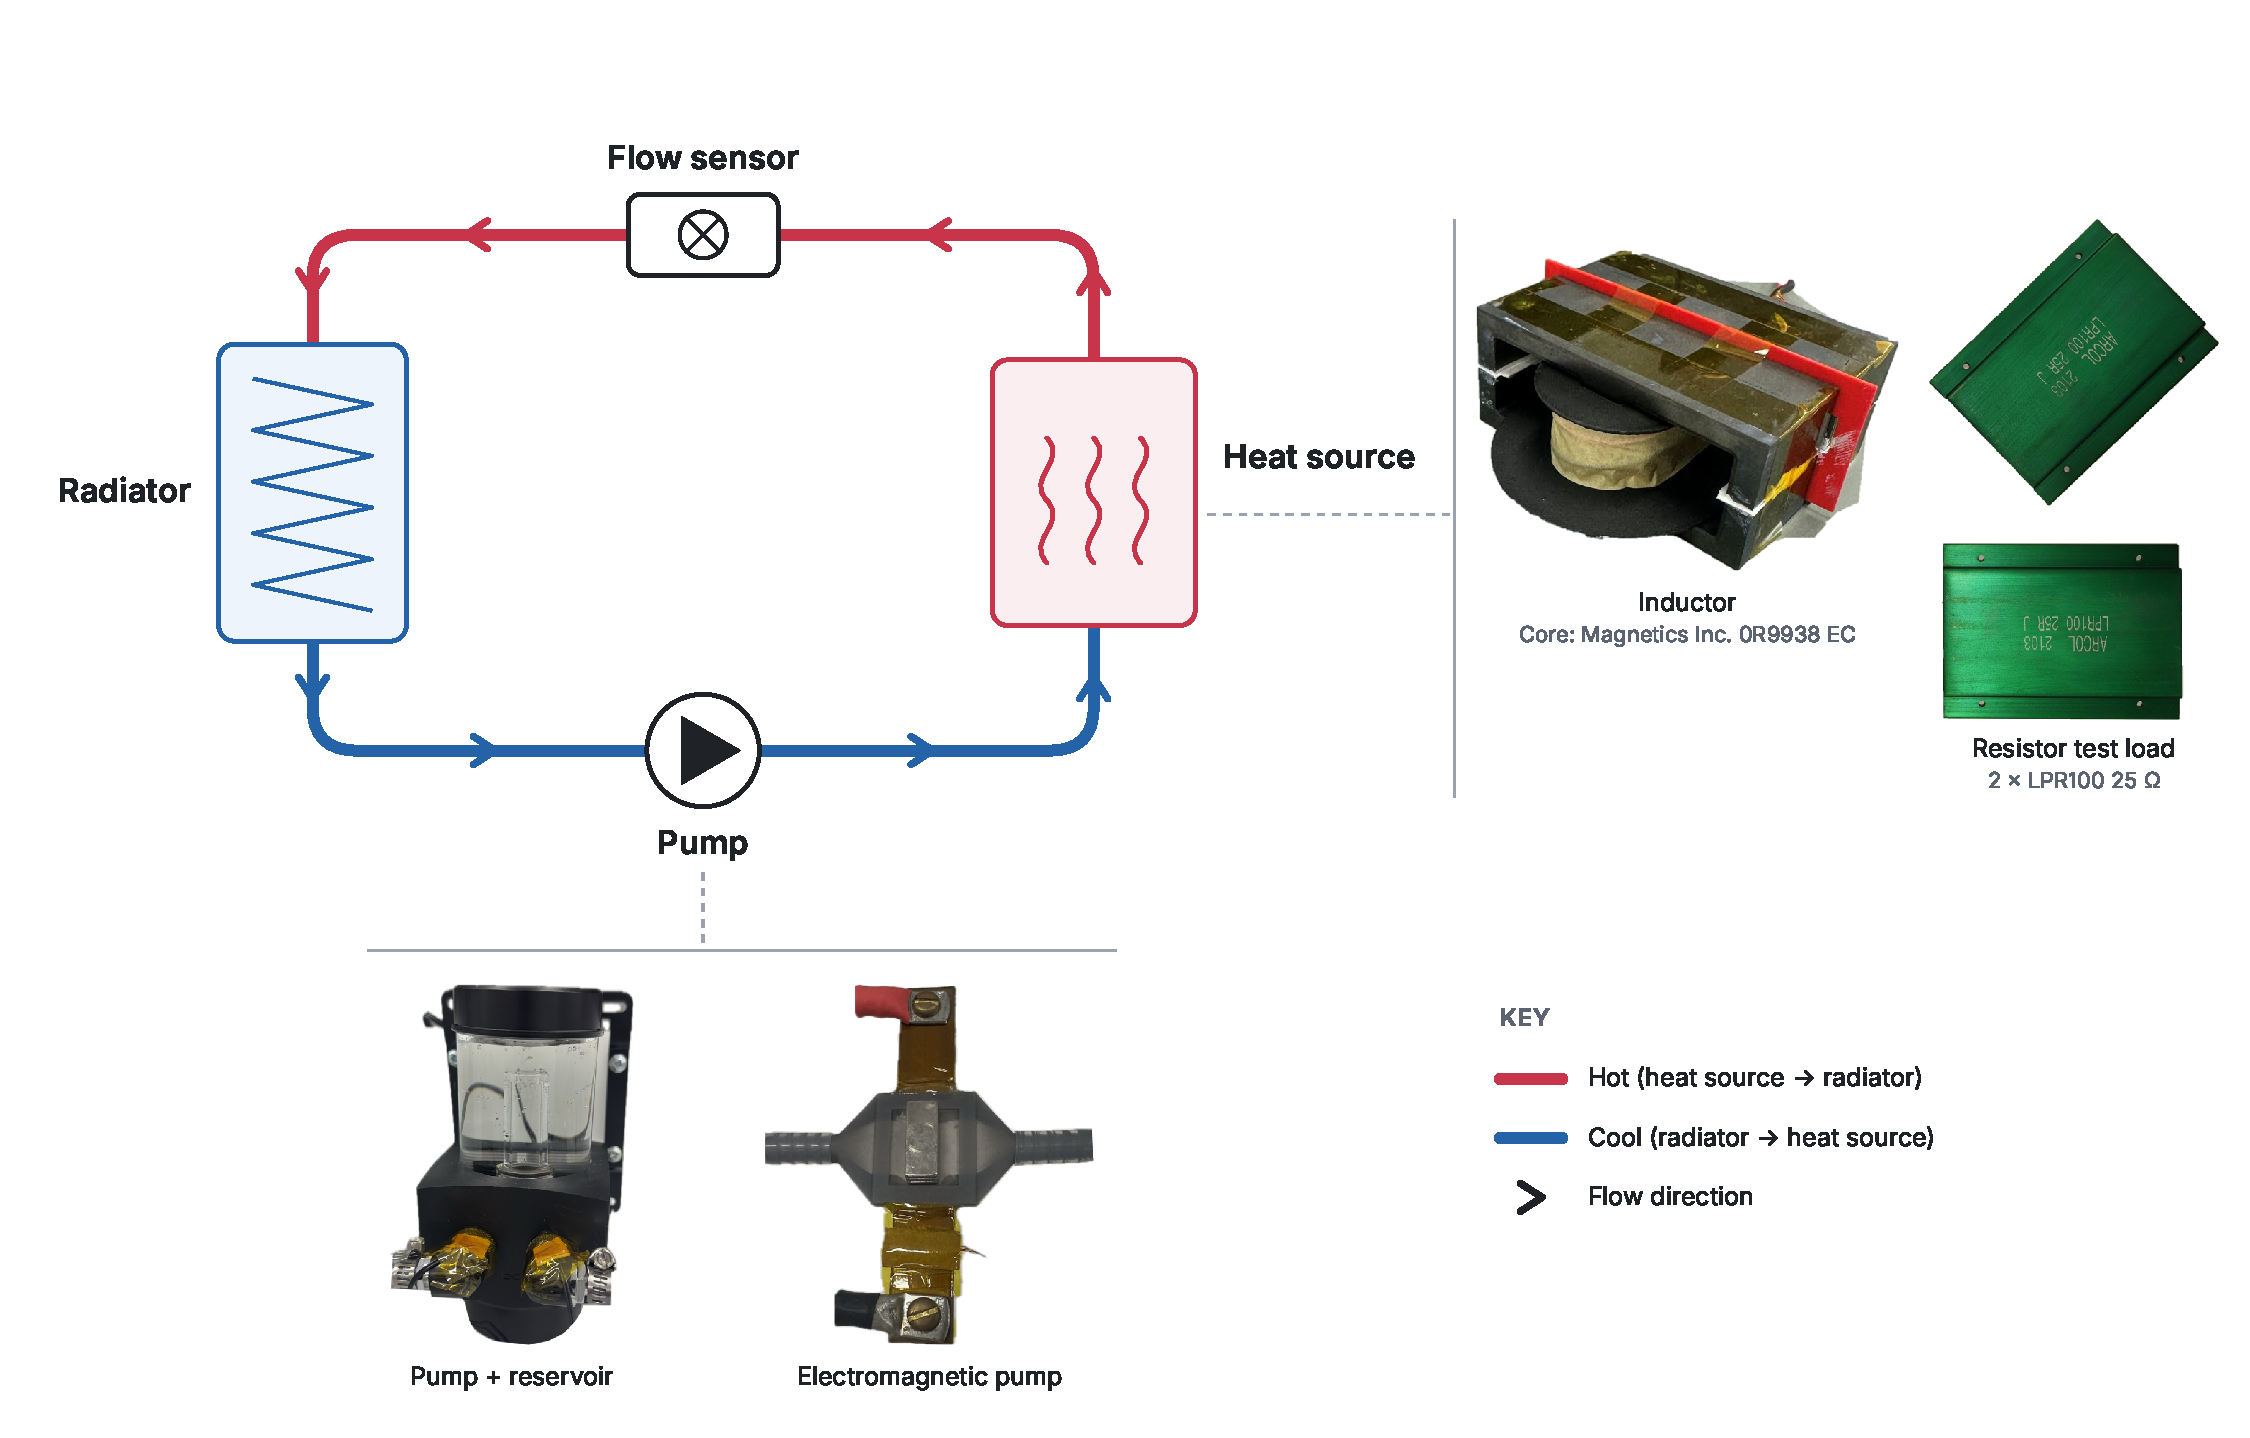
\includegraphics[width=0.85\linewidth]{figures/cooling_loop.pdf}
  \caption{Cooling loop arrangement shared by the Galinstan and water systems.
    The coolant is pumped through the heat source (resistor test load or
    inductor), past the flow sensor and through the radiator before returning
    to the pump. The water loop uses a pump with an integrated reservoir; the
    Galinstan loop uses an electromagnetic pump.}
  \label{fig:cooling-loop}
\end{figure}

The Galinstan loop is the apparatus constructed by the 2025 Part~IV Project~\#51
group~\cite{kwon_project_2025,loh_project_2025}. Galinstan is circulated by a
permanent-magnet DC conduction pump, in which a current passed through the
coolant between two copper electrodes produces a Lorentz force
(\cref{sec:em-pumping}). The pump is supplied by a XANTREX XKW~60--18 DC power
supply, which provides up to \SI{18}{\ampere}. PFA tubing carries the coolant
to an ATS-TCP-1001 tubed cold plate and back through an ATS-TCP-1003 cold plate
fitted with a heat sink and two fans, which acts as the
radiator~\cite{kwon_project_2025,advanced_thermal_solutions_inc_tubed_2021}.
Conventional mechanical flow meters are not compatible with Galinstan, so the
flow rate is measured with an electromagnetic flow sensor of the same
construction as the pump. The flowing coolant induces an EMF $E$ across the
sensor electrodes, from which the volumetric flow rate is $\Vdot = Eh/B$, where
$h$ is the channel height and $B$ the magnetic flux density across the
channel~\cite{kwon_project_2025}.

The water loop was designed and built by the project partner, Ekbote, to
replicate the Galinstan apparatus, and its design is detailed in Ekbote's
project report~\cite{ekbote_project_2026}. It uses the same model of tubed cold
plate (ATS-TCP-1001), so that the two
coolants are compared through an identical cold-plate geometry
(\cref{tab:coolant-properties}). The water is circulated by a pump with an
integrated reservoir, whose speed is set by the duty cycle of its drive signal,
and the flow rate is read directly from a Sea Zhongjiang digital flow meter. A
valve was later added to the water loop to reduce the flow below the
controllable range of the pump. The two loops therefore share the heat source
and the cold-plate geometry, but differ in the pump, the achievable flow range
and the method of flow measurement.

\subsection{Heat Sources}
\label{sec:heat-sources}

Two heat sources were used. For the first experiment, heat was applied by two
\SI{100}{\watt}, \SI{25}{\ohm} ARCOL LPR100 resistors mounted side by side on the
cold plate with a thermal interface material. The resistors were connected in
series and supplied by a GW Instek GPE-3323 DC power supply, so that the
dissipated power could be read directly from the supply. A heat load of
\SI{72}{\watt} (\SI{60}{\volt} across the \SI{50}{\ohm} pair) was used for most
tests, the same load used in~\cite{kwon_project_2025,loh_project_2025}. The
resistors were covered with polystyrene insulation to reduce the heat lost to
the environment. For the second experiment, the resistors were replaced by a
power-dense planar inductor, whose design is described in
\cref{sec:inductor-design}.

\subsection{Instrumentation}
\label{sec:instrumentation}

Galinstan is corrosive to many commonly used sensor materials, which restricts
the range of compatible measurement devices (\cref{sec:compatibility}). System
performance was therefore evaluated using the limited set of measurements
summarised in \cref{tab:measurements}. Temperatures around each loop were
logged continuously by a thermistor data-acquisition system adapted
from~\cite{kwon_project_2025,loh_project_2025}. At steady state, K-type
thermocouples, with an accuracy of $\pm\SI{2.2}{\celsius}$~\cite{loh_project_2025},
were used as the reference temperatures at the resistor, the cold-plate inlet
and the cold-plate outlet. A thermal camera was used where available, chiefly
for the inductor experiment.

\begin{table}[htbp]
  \centering
  \caption{Measured quantities and instrumentation.}
  \label{tab:measurements}
  \small
  \begin{tabularx}{\linewidth}{@{}>{\raggedright\arraybackslash}p{2.7cm}
      >{\raggedright\arraybackslash}p{4.1cm} L@{}}
    \toprule
    Quantity & Description & Method \\
    \midrule
    \multirow[t]{2}{=}{Heat load}
      & Power dissipated by the resistors.
      & Read from the GW Instek GPE-3323 DC power supply. \\
      & Power dissipated in the inductor.
      & Estimated from the core-loss model and the measured AC resistance
        (\cref{sec:model-validation}). \\
    \midrule
    \multirow[t]{2}{=}{Volumetric flow rate, $\Vdot$}
      & Galinstan loop.
      & EMF $E$ of the electromagnetic flow sensor, read with an Agilent 34410A
        digital multimeter; $\Vdot = Eh/B$~\cite{kwon_project_2025}. \\
      & Water loop.
      & Read directly from the Sea Zhongjiang digital flow meter. \\
    \midrule
    Temperature
      & Thermistors around the loop and, at steady state, thermocouples at the
        resistor, cold-plate inlet and cold-plate outlet.
      & Data-acquisition system adapted from~\cite{kwon_project_2025,loh_project_2025};
        thermal camera where available. \\
    \midrule
    Pump power
      & Electrical input power to each pump.
      & Voltage across the pump terminals and current from each pump's DC
        power supply. \\
    \midrule
    AC resistance, $R_{\mathrm{ac}}$
      & Series resistance of the inductor winding.
      & Agilent E4980A LCR meter (\cref{sec:exp2}). \\
    \midrule
    Pump volume
      & Volume occupied by each pump.
      & Physical measurement, supplemented by CAD dimensions where physical
        measurement is impractical. \\
    \bottomrule
  \end{tabularx}
\end{table}

\subsection{Safety Considerations}
\label{sec:safety}

The safety of project members and other laboratory users was prioritised
throughout the experimental setup and operation. Every experiment was set up by
two project members, and all connections were cross-checked with the project
partner before the system was energised. While temperatures exceeded
\SI{38}{\celsius}, the apparatus was continuously monitored by at least one
project member, and no one was permitted to interact with the system while it
was live. All electrical terminals operating above \SI{50}{\volt} DC were
covered, and the inverter and resonant tank used in the second experiment were
fully enclosed in acrylic boxes. Protective eyewear was worn, and physical
barriers prevented accidental contact with the live system. At shutdown, the
heat source was switched off first while the coolant continued to circulate,
and the apparatus was supervised for at least 30 minutes, until it had cooled
below \SI{38}{\celsius}.

% ---------------------------------------------------------------------
\section{Inductor Design}
\label{sec:inductor-design}

Cooling systems for magnetic components sit in their leakage fields
(\cref{sec:form-factor}), which could heat a Galinstan coolant. An initial ANSYS
simulation, with the Galinstan modelled as a stationary solid, found it 3.2
times as lossy as aluminium and almost 3.9 times as lossy as copper, and showed
that \SI{1}{\milli\metre} of copper shielding reduced the total loss by over
\SI{70}{\percent}. To measure this effect, a power-dense inductor that requires
active cooling was built and placed on the Galinstan cold plate. It operates at
\SI{85}{\kilo\hertz}~\cite{society_of_automotive_engineers_r_2024}, so that its
leakage field is representative of IPT magnetics (\cref{sec:ipt-losses}), and
uses a planar geometry, which offers better thermal performance than
alternatives such as pot cores. The final construction is shown in
\cref{fig:inductor-photo}.

\subsection{Analytical and Numerical Design}
\label{sec:analytical-design}

To reduce computation time and narrow the design space, an analytical model was
developed before the numerical simulations. This initial model assumed a
two-part construction of TDK N85 ferrite ELP-type cores, and swept the air-gap
length (\SIrange{0.5}{1.5}{\milli\metre}) and the number of turns (8--12). The
core loss of each design was estimated with the Steinmetz equation, which
expresses the loss per unit volume as a power law in frequency and peak flux
density~\cite{li_review_2022}. The model identified designs whose loss exceeds
the core's datasheet loss limit of
\SI{17.88}{\watt}~\cite{magnetics_inc_specification_2005}, so that active
cooling is required, while keeping the peak flux density below about
\SI{300}{\milli\tesla}.

An ANSYS model was then constructed and run as a two-parameter sweep over
air-gap length and number of turns. It was later found that the available cores
were Magnetics Inc.\ Material~R rather than the assumed TDK N85. A custom
material definition was therefore created by modifying the properties of TDK
N95, which are similar to those of Material~R. The core material was assumed to
operate at \SI{65}{\celsius}, the target steady-state operating temperature for
the experiments. With the material defined, a parameter sweep (8--12 turns,
\SIrange{0.5}{1.2}{\milli\metre} air gap) was performed to extract the
inductance and core loss.

To finalise the design, the flux density in the core was checked and found to
be acceptable, within the linear region of operation (\cref{fig:flux-density}).
The final design parameters, including the inductance and core loss of the
chosen design, are given in \cref{tab:inductor-design}.

\begin{figure}[htbp]
  \centering
  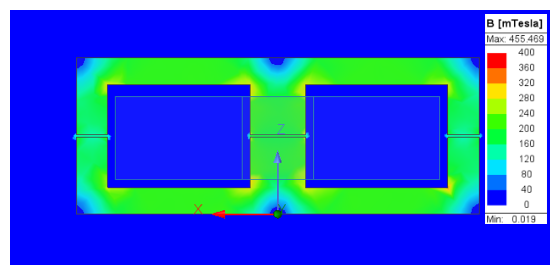
\includegraphics[width=0.72\linewidth]{inductor_flux_density}
  \caption{Magnetic flux density in the selected inductor design ($N = 8$,
    $l_{\mathrm{g}} = \SI{0.6}{\milli\metre}$).}
  \label{fig:flux-density}
\end{figure}

\begin{table}[htbp]
  \centering
  \caption{Final inductor parameters from the ANSYS model at the rated current
    of \SI{12}{\ampere} rms.}
  \label{tab:inductor-design}
  \begin{tabular}{@{}lll@{}}
    \toprule
    Parameter & Value & Unit \\
    \midrule
    Core geometry  & Magnetics Inc.\ 0\,9938\,EC & -- \\
    Core material  & Magnetics Inc.\ Material~R  & -- \\
    Air-gap length & 0.6   & \si{\milli\metre} \\
    Turns          & 8     & -- \\
    Inductance     & 92.5  & \si{\micro\henry} \\
    Core loss      & 30.81 & \si{\watt} \\
    \bottomrule
  \end{tabular}
\end{table}

\subsection{Model Validation}
\label{sec:model-validation}

Once the inductor had been built (\cref{fig:inductor-photo}), measurements were
taken to design the LCC tuning required to drive the desired resonant current.
These measurements also serve to validate the model, whose values at the rated
current of \SI{12}{\ampere} rms are given in \cref{tab:inductor-design}.

\begin{figure}[htbp]
  \centering
  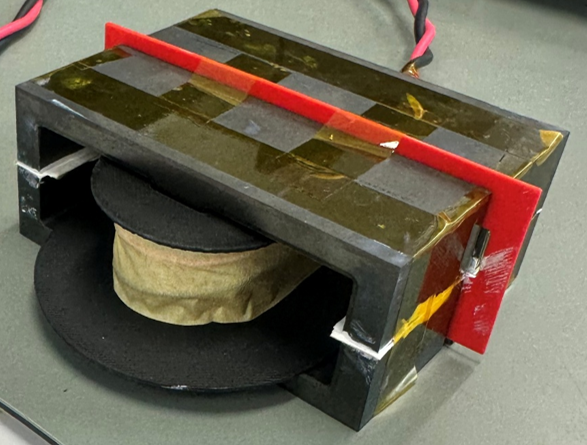
\includegraphics[width=0.42\linewidth]{inductor_photo}
  \caption{Constructed planar inductor.}
  \label{fig:inductor-photo}
\end{figure}

The inductance was measured as \SI{92.1}{\micro\henry}, within \SI{1}{\percent}
of the simulation model, although this measurement included the effect of long
leads, which would be expected to increase it. The AC resistance
$R_{\mathrm{ac}}$, which determines the winding loss, was measured with an LCR
meter at low excitation as \SI{83}{\milli\ohm}, giving a winding loss of
\SI{11.95}{\watt} at \SI{12}{\ampere} rms.

For a heat transfer investigation in which temperatures are continuously
monitored, some uncertainty in the loss estimate is acceptable. For the later
experiments, the total inductor loss is therefore taken as \SI{42.76}{\watt}
(\SI{30.81}{\watt} core loss plus \SI{11.95}{\watt} winding loss).

\subsection{Thermal Considerations and Cooling Strategy}
\label{sec:inductor-thermal}

The main constraint was asymmetric cooling. The upper core relies on convection
to ambient air, while the lower core sits on the cold plate, and the air gap
between them acts as a thermal insulator. Thermal paste was applied between the
upper and lower cores to reduce the temperature difference and improve heat
transfer to the cooling system. Although not optimal, this configuration is
suitable for the second experiment, which aims to demonstrate Galinstan cooling
of a power-dense inductor and to assess the leakage-field interaction rather
than to produce the best-performing system. Future work could improve the design
by cooling both the top and bottom cores, or by using asymmetric core designs
with an integrated heat-transfer path, such as the inductor of Gao
\emph{et al.}~\cite{gao_modeling_2022}.

\subsection{Capacitor Tuning}
\label{sec:capacitor-tuning}

The allowable reactance of the inductor was limited by the maximum voltage
developed across the series tuning capacitors needed to boost the volt-amperes
(VA) in the inductor, which was limited to \SI{150}{\volt} across any single
capacitor. To find
acceptable tuning values, an optimisation model was developed using the Solver
add-in in Microsoft Excel, which made it possible to check quickly whether a
given inductance was feasible or would cause the capacitor voltage to exceed its
rating.

The target capacitance is given by
\begin{equation}
  C_{\mathrm{target}} = \frac{1}{2\pi f \left(2\pi f L_{1} - X_{\mathrm{res}}\right)},
  \label{eq:c-target}
\end{equation}
where $f$ is the resonant frequency of the network (\SI{85}{\kilo\hertz}),
$L_{1}$ is the inductance of the primary magnetics and $X_{\mathrm{res}}$ is the
resonant reactance of the system. $X_{\mathrm{res}}$ sets the resonant current in
the primary magnetics, as given by
\begin{equation}
  X_{\mathrm{res}} = \frac{2\sqrt{2}\, V_{\mathrm{DC}}}{\pi I_{1}},
  \label{eq:x-res}
\end{equation}
where $I_{1}$ is the desired resonant current and $V_{\mathrm{DC}}$ is the DC bus
voltage, here \SI{60}{\volt}. \Cref{eq:x-res} is valid only for a conduction
angle of \SI{180}{\degree}. With the measured inductance of \SI{92.1}{\micro\henry} and a resonant current of
\SI{12}{\ampere}, \cref{eq:c-target,eq:x-res} give a target capacitance of
\SI{41.90}{\nano\farad}.

Initially, the optimisation model selected a single capacitor value for the
entire board. The result was relatively poor, with the best design differing by
\SI{8.11}{\percent} from the target capacitance. The model was then extended to
allow one value from a limited set (\SIlist{22;68;100}{\nano\farad}) to be
selected for each of the four series-connected rows of the tuning board, with up
to 14 capacitors in parallel per row. This reduced the detuning to
\SI{2.12}{\percent} of the target value. The final arrangement, with the voltage
across each row at the rated current, is given in \cref{tab:capacitor-opt}. The
highest row voltage is about \SI{146}{\volt}, within the \SI{150}{\volt} limit.

\begin{table}[htbp]
  \centering
  \caption{Final arrangement of the series tuning capacitors from the
    optimisation model. The four rows are connected in series; row voltages are
    at \SI{12}{\ampere} rms and \SI{85}{\kilo\hertz}.}
  \label{tab:capacitor-opt}
  \small
  \begin{tabular}{@{}lcccc@{}}
    \toprule
    Row & Capacitor value & Number in parallel & Row capacitance & Row voltage \\
        & (\si{\nano\farad}) & & (\si{\nano\farad}) & (\si{\volt}) \\
    \midrule
    1 & 22 & 7 & 154 & 145.9 \\
    2 & 68 & 3 & 204 & 110.1 \\
    3 & 22 & 7 & 154 & 145.9 \\
    4 & 22 & 7 & 154 & 145.9 \\
    \midrule
    \multicolumn{3}{@{}l}{Target capacitance}   & 41.90 & \\
    \multicolumn{3}{@{}l}{Achieved capacitance} & 41.01 & \\
    \multicolumn{3}{@{}l}{Error}                & 0.89 (\SI{2.12}{\percent}) & \\
    \bottomrule
  \end{tabular}
\end{table}

% ---------------------------------------------------------------------
\section{Thermal Modelling}
\label{sec:thermal-model}

Thermal models were developed alongside the experiments, both to interpret the
measurements and to extend them beyond the conditions the apparatus could reach.
This section first presents a lumped thermal network and the $\varepsilon$--NTU
analysis used to calculate its cold-plate resistance, followed by the convection
correlations and test conditions it relies on. A conjugate heat transfer
simulation, which resolves the temperature field that the network lumps
together, is then described. The models are compared with the measurements in
\cref{ch:results}.

\subsection{Thermal Network}
\label{sec:thermal-network}

Following the analyses of Kwon~\cite{kwon_project_2025} and
Loh~\cite{loh_project_2025}, the input heat $\Qin$ divides at the resistor node
$\Tres$, as shown in \cref{fig:thermal-network}. Part of the heat is
lost to ambient through $\Rmisc$. The rest, $\Qplate$, passes through the
package resistance $\Rpack$ (resistor and thermal interface) to a fictitious
isothermal plate node $T_{\mathrm{P}}$, and then through the cold-plate
resistance $\Rcp$ to the coolant inlet:
\begin{equation}
  \Qin = \frac{\Tres - T_{\mathrm{A}}}{\Rmisc}
       + \frac{\Tres - \Tin}{\Rpack + \Rcp}.
  \label{eq:network}
\end{equation}
The resistance to ambient $\Rmisc$ was found for each loop from a no-flow test
at a heat load of \SI{12}{\watt}. With no coolant flow, the heat input is lost
to the environment, so
\begin{equation}
  \Rmisc = \frac{\Tres - T_{\mathrm{A}}}{\Qin}.
  \label{eq:rmisc}
\end{equation}
This resistance was then used to calculate the loss to the environment at any
resistor temperature. For the Galinstan loop, $T_{\mathrm{A}} =
\SI{20.5}{\celsius}$ and $\Rmisc = \SI{3.33}{\celsius\per\watt}$; for the water
loop, $T_{\mathrm{A}} = \SI{21.6}{\celsius}$ and
$\Rmisc = \SI{2.95}{\celsius\per\watt}$. With these values, between
\SI{9}{\watt} and \SI{12}{\watt} of the heat load is lost to the environment in
each test (\cref{tab:measured-performance}). This network was used in all the
following models.
\issue{\Cref{fig:thermal-network} still labels the resistor node
$T_{\mathrm{M}}$; update the image to $T_{\mathrm{resistor}}$.}

\begin{figure}[htbp]
  \centering
  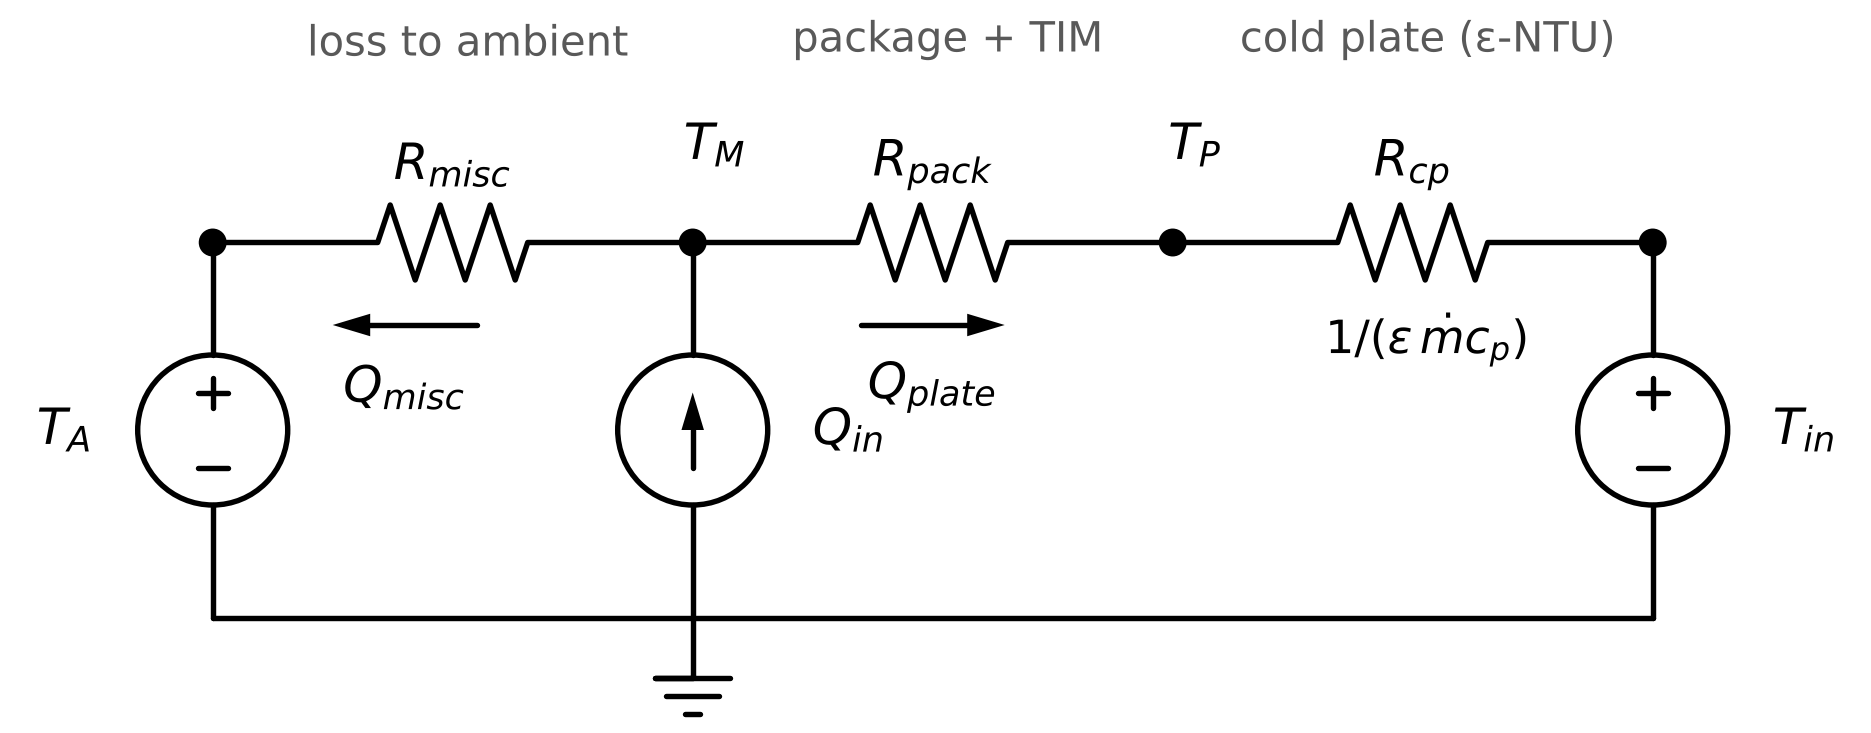
\includegraphics[width=0.85\linewidth]{thermal_network}
  \caption{Thermal network as an electrical analogue (temperature $\equiv$
    potential, heat flow $\equiv$ current); $T_{\mathrm{A}}$ and $\Tin$ are fixed
    boundary conditions.}
  \label{fig:thermal-network}
\end{figure}

\subsection{\texorpdfstring{$\varepsilon$--NTU}{epsilon-NTU} Analysis of the Cold Plate}
\label{sec:eps-ntu}

For this analysis, the plate is considered isothermal at $T_{\mathrm{P}}$, so
coolant entering at $\Tin$ approaches the plate temperature exponentially. An
energy balance on a tube element of perimeter $P$ gives~\cite{bergman_fundamentals_2017}
\begin{equation}
  \frac{T_{\mathrm{P}} - T_{\mathrm{f}}(x)}{T_{\mathrm{P}} - \Tin}
    = \exp\!\left(-\frac{hPx}{\mdot\,\cp}\right).
  \label{eq:temp-profile}
\end{equation}
At the outlet ($x = L$, $PL = A$), the exponent is defined as the number of
transfer units, $\NTU = hA/(\mdot\,\cp)$. This is the ratio of the
wall-to-coolant convective conductance to the heat-capacity rate of the coolant.
Each transfer unit reduces the remaining plate-to-coolant temperature difference
by a factor of $e$, so the coolant absorbs about \SI{63}{\percent} of the maximum
possible heat after one transfer unit~\cite{bergman_fundamentals_2017}. Defining
the effectiveness $\varepsilon$ as this fraction gives
\begin{equation}
  \Qplate = \varepsilon\,\mdot\,\cp\,(T_{\mathrm{P}} - \Tin), \qquad
  \varepsilon = 1 - e^{-\NTU}, \qquad
  \Rcp = \frac{1}{\varepsilon\,\mdot\,\cp},
  \label{eq:effectiveness}
\end{equation}
\begin{equation}
  T_{\mathrm{P}} = \Tin + \Qplate\Rcp, \qquad
  \Tout = \Tin + \frac{\Qplate}{\mdot\,\cp}.
  \label{eq:plate-outlet}
\end{equation}
This is the effectiveness relation for one flow stream against an isothermal
surface~\cite{bergman_fundamentals_2017}. Its limits show whether a coolant is
limited by convection at the wall or by its ability to transport heat
(caloric-limited), as summarised in \cref{tab:ntu-regimes}.

\begin{table}[htbp]
  \centering
  \caption{Limiting regimes of the $\varepsilon$--NTU relation for an isothermal
    plate.}
  \label{tab:ntu-regimes}
  \small
  \begin{tabular}{@{}lllll@{}}
    \toprule
    Regime & NTU & $\varepsilon$ & $\Rcp$ & Lever to reduce $\Rcp$ \\
    \midrule
    Convection-limited & $\ll 1$ & $\approx \NTU$ &
      $\approx 1/(hA) + 1/(2\mdot\,\cp)$ & Raise $hA$ (Nu, area) \\
    Transitional & $\approx 1$ & $1 - e^{-\NTU}$ &
      $1/(\varepsilon\,\mdot\,\cp)$ & Both \\
    Caloric-limited & $\gg 1$ ($\gtrsim 3$) & $\to 1$ &
      $\to 1/(\mdot\,\cp)$ & Raise $\mdot\,\cp$ (flow rate) \\
    \bottomrule
  \end{tabular}
\end{table}

The isothermal-plate assumption relies on in-plane heat spreading within the
\SI{15}{\milli\metre} 6063 aluminium base (\cref{fig:coldplate-heatflow}). The
assumption weakens as the coolant temperature rise between inlet and outlet,
$\Delta T_{\mathrm{cool}} = \Qplate/(\mdot\,\cp)$, increases. The predicted rise
is below \SI{2}{\celsius} for water but approximately
\SIrange{17}{20}{\celsius} for Galinstan, so the model is expected to describe
water better than Galinstan. For this reason, the package resistance $\Rpack$
was calibrated on the two turbulent water tests, which give the most nearly
isothermal plate, as \SI{0.242}{\celsius\per\watt}. It was then held at this
value for all flows and both coolants.

\begin{figure}[htbp]
  \centering
  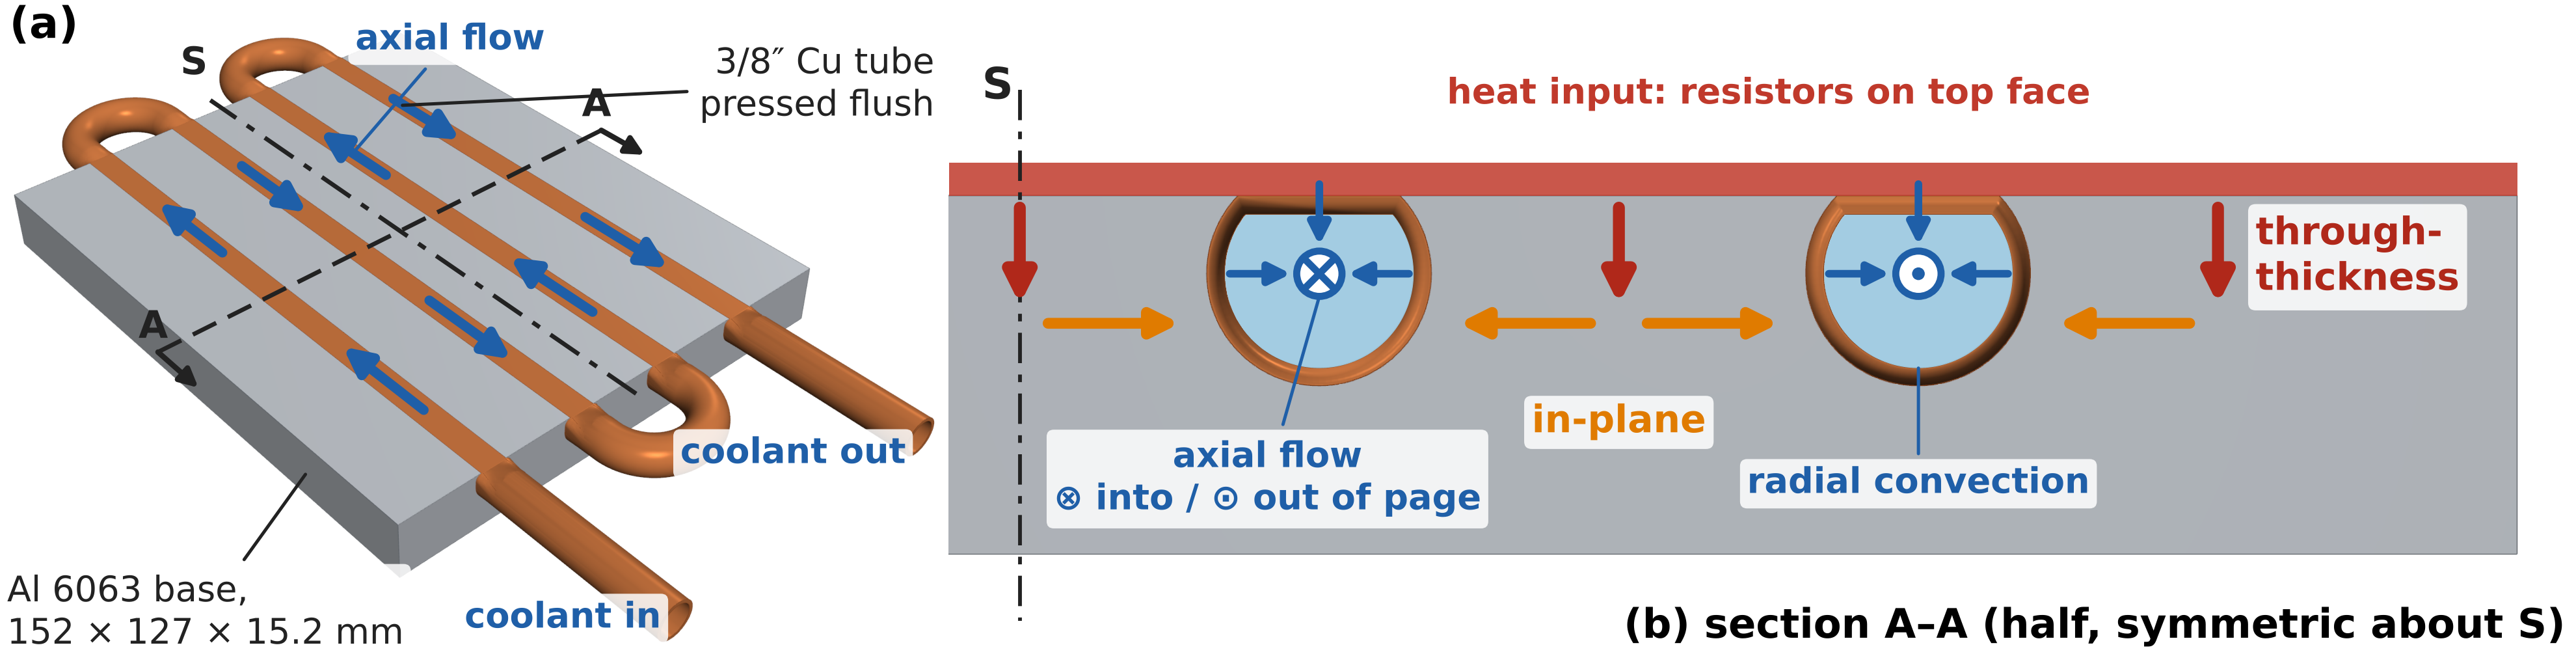
\includegraphics[width=0.85\linewidth]{coldplate_heat_flow}
  \caption{Heat-flow directions in the cold plate: in-plane spreading (plate),
    through-thickness conduction (part of $\Rpack$), axial flow and radial
    convection ($R_{\mathrm{conv}}$).}
  \label{fig:coldplate-heatflow}
\end{figure}

\subsection{Convection Correlations and Test Conditions}
\label{sec:convection}

The $\varepsilon$--NTU model requires an estimate of the heat transfer
coefficient $h$ between the tube wall and the coolant. It is obtained from
standard correlations for the Nusselt number, $\mathrm{Nu} = hD/k$, a
dimensionless measure of how effectively the flowing coolant removes heat from
the wall. For laminar flow, the Shah and London
correlation~\cite{shah_laminar_1978} gives the mean Nu along a tube at constant
wall temperature, including the thermal entry region where heat transfer is
highest. It is applied to each \SI{152}{\milli\metre} pass separately, on the
assumption that the U-bends mix the flow. For turbulent water
($\mathrm{Re} \geq 4000$), Gnielinski's correlation~\cite{bergman_fundamentals_2017}
is used, and no estimate is made in the transitional range
$2300 < \mathrm{Re} < 4000$. Galinstan remains laminar up to
\SI{5}{\milli\litre\per\second} ($\mathrm{Re} \leq 2110$). The correlations and
worked calculations for both coolants are given in \cref{app:convection}.

The NTU analysis uses these correlations for both coolants. For the turbulent
water tests, however, the cold-plate resistance given in the ATS-TCP-1001
datasheet~\cite{advanced_thermal_solutions_inc_tubed_2021} was later found to
fit the measured data better, so the temperature predictions for these tests
use the datasheet values, fitted as
$\Rcp = 0.0274\,\Vdot^{-0.415}$~\si{\kelvin\per\watt} ($\Vdot$ in
\si{\litre\per\minute}). The Galinstan and laminar water tests use the
$\varepsilon$--NTU model.
\Cref{tab:coolant-properties,tab:tests} summarise the cold-plate geometry, the
coolant properties and the test conditions.

\begin{table}[htbp]
  \centering
  \caption{Cold-plate geometry (ATS-TCP-1001) and coolant properties.}
  \label{tab:coolant-properties}
  \small
  \begin{tabularx}{\linewidth}{@{}>{\raggedright\arraybackslash}p{4.3cm}ll L@{}}
    \toprule
    Quantity & Galinstan & Water & Note \\
    \midrule
    Tube bore / heated length per pass & \SI{8}{\milli\metre} / \SI{152}{\milli\metre}
      & \SI{8}{\milli\metre} / \SI{152}{\milli\metre}
      & Bore measured; plate length and 4 passes
        from~\cite{advanced_thermal_solutions_inc_tubed_2021};
        $A = \SI{0.0153}{\metre\squared}$ \\
    $\rho$ (\si{\kilogram\per\metre\cubed}) / $\cp$ (\si{\joule\per\kilogram\per\kelvin})
      & 6370 / 366 & 1000 / 4182
      & Galinstan $\rho$~\cite{kwon_project_2025}, $\cp$~\cite{zhang_experimental_2019} \\
    $k$ (\si{\watt\per\metre\per\kelvin}) / $\mu$ (\si{\milli\pascal\second})
      & 16.5 / 2.4 & 0.60 / 1.0 & \cite{kwon_project_2025} \\
    \bottomrule
  \end{tabularx}
\end{table}

\begin{table}[htbp]
  \centering
  \caption{Steady-state tests, estimated coolant temperature rise and cold-plate
    resistance used in the predictions.}
  \label{tab:tests}
  \small
  \setlength{\tabcolsep}{4.5pt}
  \begin{tabular}{@{}llrrlrr@{}}
    \toprule
    Test & Flow & $\Qin$ (\si{\watt}) & Re & Regime &
      $\Delta T_\mathrm{cool}$ (\si{\celsius}) & $R_\mathrm{cp}$ (\si{\celsius\per\watt}) \\
    \midrule
    Galinstan, full (\SI{18}{\ampere}) & \SI{1.4}{\milli\litre\per\second}  & 72 & 591  & Laminar   & 17.8\textsuperscript{\textdagger} & 0.295 \\
    Galinstan, low (\SI{9}{\ampere})   & \SI{0.75}{\milli\litre\per\second} & 40 & 317  & Laminar   & 17.1\textsuperscript{\textdagger} & 0.555 \\
    Water & \SI{3.5}{\litre\per\minute}  & 72 & 9284 & Turbulent & 0.26 & 0.016\textsuperscript{\textdaggerdbl} \\
    Water & \SI{1.75}{\litre\per\minute} & 72 & 4642 & Turbulent & 0.52 & 0.022\textsuperscript{\textdaggerdbl} \\
    Water & \SI{0.73}{\litre\per\minute} & 72 & 1936 & Laminar   & 1.22 & 0.074 \\
    Water & \SI{0.5}{\litre\per\minute}  & 72 & 1326 & Laminar   & 1.78 & 0.088 \\
    \bottomrule
    \multicolumn{7}{@{}p{\linewidth}@{}}{\footnotesize
      $\Delta T_\mathrm{cool} = Q_\mathrm{plate}/(\mdot\,\cp)$, where
      $Q_\mathrm{plate}$ is $\Qin$ less the loss to ambient through
      $R_\mathrm{misc}$. $R_\mathrm{cp}$ is from the $\varepsilon$--NTU model
      unless marked.
      \textsuperscript{\textdagger}\,Galinstan $\mdot\,\cp$ estimated from the
      energy balance, so $\Delta T_\mathrm{cool}$ equals the measured
      $T_\mathrm{out} - T_\mathrm{in}$; nominal flows are from the EMF
      flow sensor.
      \textsuperscript{\textdaggerdbl}\,ATS datasheet
      fit~\cite{advanced_thermal_solutions_inc_tubed_2021};
      \SI{1.75}{\litre\per\minute} is slightly extrapolated below the lowest
      datasheet point (\SI{1.89}{\litre\per\minute}).}
  \end{tabular}
\end{table}
\edited{Turbulent water flows changed from 3.6 and \SI{1.8}{\litre\per\minute}
to the measured 3.5 and \SI{1.75}{\litre\per\minute} (58.3 and
\SI{29.2}{\milli\litre\per\second}) here and in later chapters. Re and
$\Delta T_{\mathrm{cool}}$ were recalculated; $\Rcp$, NTU, $\Rpack$ and the
predicted temperatures are unchanged at the precision shown (the datasheet
$\Rcp$ changes by \SI{0.0002}{\celsius\per\watt}). Thermal\_Network\_Model.xlsx
still uses 3.6 and \SI{1.8}{\litre\per\minute}.}

\subsection{Conjugate Heat Transfer Simulation}
\label{sec:cht}

The thermal network reproduces the measured resistor temperatures by lumping the
cold plate into a single isothermal node. This is reasonable for water, but for
Galinstan the plate is not isothermal. The network also cannot resolve how heat
spreads from the discrete resistor footprints through the press-fit tube
contact, nor capture flow redevelopment at the U-bends or the transitional flow
suspected in the low-flow water tests. A conjugate heat transfer (CHT)
simulation, which solves the coolant flow and the conduction through the solids
together, was therefore completed in SimScale~\cite{simscale_gmbh_simscale_2021}.
It resolves the temperature fields in the plate and coolant, and the local peak
temperatures that govern component and insulation limits.

To reduce computation time, a simplified model of the cold plate was first
created in Onshape~\cite{ptc_onshape_2015} and imported into SimScale
(\cref{fig:cfd_setup}). An internal flow volume was then defined in the
geometry. The solids were assigned SimScale's default material properties for
aluminium and copper, and water used the default material. A custom Galinstan
material was created from the properties in \cref{tab:coolant-properties}. The
simulation settings and boundary conditions are summarised in
\cref{tab:simulation-setup}, and parameters not listed were left at their
default values.

\begin{figure}[htbp]
    \centering
    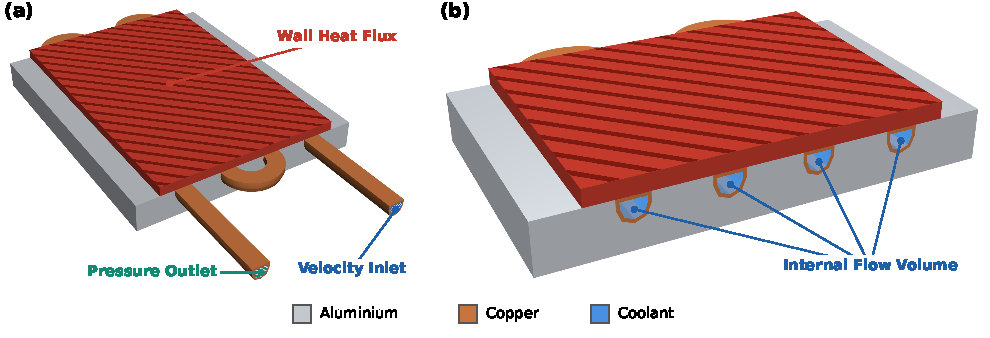
\includegraphics[width=\textwidth]{coldplate_figure.pdf}
    \caption{Cold-plate model used for the CHT analysis.
        (a)~Isometric view and (b)~cut showing the internal flow volume.}
    \label{fig:cfd_setup}
\end{figure}

The boundary conditions were chosen to match each test. The inlet was set as a
velocity inlet at the measured inlet temperature of the test (for example,
\SI{29.8}{\celsius} for the full-flow Galinstan test), with the velocity
adjusted to give the measured flow rate. The outlet was held at a pressure of
\SI{1}{atm}. The heat input was applied as a heat flux equal to the heat
reaching the cold plate, $\Qplate$, rather than the full electrical input,
because part of the input is lost to the environment
(\cref{sec:thermal-network}). For the full-flow Galinstan test this was about
\SI{60}{\watt} of the \SI{72}{\watt} input, and for the low-flow Galinstan test
about \SI{30}{\watt} of the \SI{40}{\watt} input, estimated from the measured
coolant temperature rise. The water run used the same $\Qplate$ as the water
tests, about \SI{62.6}{\watt}.

\begin{table}[htbp]
  \centering
  \caption{CHT simulation settings and boundary conditions.}
  \label{tab:simulation-setup}
  \small
  \begin{tabular}{@{}ll@{}}
    \toprule
    Parameter & Setting \\
    \midrule
    Analysis type    & Conjugate heat transfer \\
    Compressible     & Yes \\
    Flow model       & $k$--$\omega$ SST (turbulent); laminar for $\mathrm{Re} \leq 2110$ \\
    Time dependency  & Steady state \\
    Inlet            & Velocity inlet at the measured flow rate and inlet temperature \\
    Outlet           & Pressure outlet, \SI{1}{atm} \\
    Heat input       & Heat flux equal to $\Qplate$ of each test at the resistor footprints \\
    Mesh             & \num{427e3} cells (\cref{app:cht_validation}) \\
    \bottomrule
  \end{tabular}
\end{table}

Turbulent cases were solved with the $k$--$\omega$ SST turbulence model, and a
laminar model was used for the runs with an estimated $\mathrm{Re} \leq 2110$.
Mesh independence was therefore assessed separately for each flow regime and
each coolant. Each study was performed at the most demanding operating point,
the highest flow rate, where the boundary layers are thinnest, so that the
resulting mesh is conservative for all milder cases. Separate studies were
needed for the two coolants because Galinstan develops a thermal boundary layer
much thicker than its velocity boundary layer, whereas water has a thermal
boundary layer thinner than its velocity boundary layer and therefore requires
finer near-wall resolution for the temperature field. The same sequence of five
meshes, from \num{73e3} to \num{1.5e6} cells, was used in every study, and the
\num{427e3}-cell mesh was adopted. The mesh study, the iterative convergence and
the comparison with experiment are given in \cref{app:cht_validation}. In
addition to the runs that reproduce each test, the cold plate was simulated
with Galinstan at four flow rates between \SI{0.75}{\milli\litre\per\second}
and \SI{5}{\milli\litre\per\second}, to compare the simulated cold-plate
resistance with the $\varepsilon$--NTU model beyond the flows the rig could
reach (\cref{sec:rcp-calc}).

\subsection{Calculation of the Cold-Plate Resistance}
\label{sec:rcp-calc}

The cold-plate resistance $\Rcp$ cannot be measured directly, because the plate
temperature $T_\mathrm{P}$ is not measured. It is therefore inferred from the
resistor and inlet temperatures by removing the package resistance from the
total resistance of the network in \cref{eq:network}:
\begin{equation}
  \Rcp = \frac{\Tres - \Tin}{Q} - \Rpack,
  \label{eq:rcp-inferred}
\end{equation}
where $\Tres$ is the mean of the left and right resistor temperatures, $Q$ is
the heat passing into the coolant and $\Rpack = \SI{0.242}{\celsius\per\watt}$
is the package resistance calibrated on the turbulent water tests. The same
definition is applied to the experimental and simulated results, so that both
are compared with the model on an equal basis (\cref{fig:galinstan_rcp_cfd}).

\paragraph{Experimental values.} $Q$ is the heat reaching the plate,
$\Qplate$, obtained by subtracting the loss to ambient through $\Rmisc$ from the
electrical input, as in \cref{eq:network}. The flow rate is taken from a
combination of the EMF flow sensor and the energy balance,
$\Vdot = \Qplate / [\rho\cp(\Tout - \Tin)]$, which agreed closely for the tests
completed in this study.

\paragraph{Simulated values.} The conjugate heat transfer results are taken at
the final iteration of each run on the \num{427e3}-cell mesh. $Q$ is obtained
from the coolant energy balance at the simulated flow rate,
\begin{equation}
  Q = \rho\cp\Vdot\,(\Tout - \Tin),
\end{equation}
which gives \SIrange{57.4}{58.2}{\watt} for all four runs, and $\Tres$ is the
mean of the two resistor probe temperatures.

\paragraph{Model values.} The $\varepsilon$--NTU model gives
$\Rcp = 1/(\varepsilon\,\mdot\,\cp)$ with $\varepsilon = 1 - e^{-\NTU}$
(\cref{sec:eps-ntu}), using the Shah and London mean Nusselt number for laminar
flow (\cref{app:convection}). Because Galinstan has $\NTU > 10$ across this
range, the model is effectively the caloric limit, $\Rcp \approx 1/(\mdot\,\cp)$.
\edited{Changed from $\NTU > 30$: the model gives $\NTU \approx 35$ at
\SI{1.4}{\milli\litre\per\second} but about 10.7 at
\SI{5}{\milli\litre\per\second}, which is still caloric-limited.}

% ---------------------------------------------------------------------
\section{Experimental Procedure}
\label{sec:programme}

Two experiments were conducted to answer the two research questions.
Experiment~1 compares the thermal performance of the water and Galinstan loops
across a range of flow rates, and its data were used to build and validate the
thermal models of \cref{sec:thermal-model}. Experiment~2 demonstrates
Galinstan's ability to cool a power-dense inductor and quantifies the
additional eddy-current loss induced in the coolant by the inductor's magnetic
field. Temperatures throughout each loop were logged continuously for the
duration of every test.

\subsection{Experiment 1: Baseline Thermal Comparison}
\label{sec:exp1}

The first experiment establishes a baseline comparison of the two cooling loops
and was run on both using identical procedures. Before each test, the data
logger was started and the coolant was circulated at the target flow rate, set
by the pump current for Galinstan and by the pump duty cycle for water. The
resistors were then switched on at the test heat load. Each test continued
until the system reached steady state, taken as a change of less than
\SI{0.5}{\celsius} over 30 minutes. The thermocouple readings at the resistor,
the cold-plate inlet and the cold-plate outlet were then recorded, together with
the flow rate and the heat load. At shutdown, the resistors were switched off
before the pump was ramped down.

The planned tests are given in \cref{tab:flow-rates}. The full-flow tests
evaluate the maximum heat transfer of the current systems, and the low-flow
tests provide data to inform and validate the thermal models. The no-flow tests,
run at a reduced heat load of \SI{12}{\watt}, measure the heat leakage to the
environment and give $\Rmisc$ (\cref{sec:thermal-network}). Two further tests
at lower flow rates,
\SI{0.73}{\litre\per\minute} and \SI{0.5}{\litre\per\minute}, were later
conducted on the water loop, using the valve to reduce the flow below the
controllable range of the pump. These give laminar water data, in the same flow
regime as Galinstan. The low-flow Galinstan test was run at a reduced heat load
of \SI{40}{\watt}, so that the resistor and the pump housing stayed below the
\SI{70}{\celsius} limit set by the resin of the MHD pump~\cite{kwon_project_2025}.

\begin{table}[htbp]
  \centering
  \caption{Planned experimental flow rates.}
  \label{tab:flow-rates}
  \small
  \begin{tabularx}{\linewidth}{@{}lccL@{}}
    \toprule
    Test & Water & Galinstan & Goal \\
    \midrule
    Full flow & \SI{58.3}{\milli\litre\per\second} & \SI{1.4}{\milli\litre\per\second}
      & Evaluate the maximum heat transfer of the current systems \\
    Low flow  & \SI{29.2}{\milli\litre\per\second} & \SI{0.8}{\milli\litre\per\second}
      & Provide data to inform and validate the thermal models \\
    No flow   & \SI{0}{\milli\litre\per\second}    & \SI{0}{\milli\litre\per\second}
      & Assess heat leakage to the environment \\
    \bottomrule
  \end{tabularx}
\end{table}

\subsection{Experiment 2: Inductor Cooling and Eddy-Current Loss}
\label{sec:exp2}

The second experiment demonstrates the ability of Galinstan to cool a
power-dense inductor and assesses the interaction between its leakage field and
the electrically conductive coolant. The thermal test follows the procedure of
Experiment~1, except that the inductor replaces the resistors. The inductor was
driven at its rated current of \SI{12}{\ampere} rms by an inverter and the
resonant tuning network of \cref{sec:capacitor-tuning}, giving an estimated heat
load of \SI{42.76}{\watt} (\cref{sec:model-validation}). The Galinstan was
operated at full flow, and the inductor temperatures were recorded with the
thermal camera. Any change in flow when the inductor was energised was captured
by the flow sensor.

The eddy-current loss induced by the leakage field was measured separately with
an Agilent E4980A LCR meter at an excitation current of about \SI{5}{\milli\ampere},
by recording the AC resistance $R_{\mathrm{ac}}$ of the inductor winding in four
configurations: (i)~the inductor alone, (ii)~the inductor on the
empty cold plate, (iii)~the inductor on the cold plate filled with Galinstan, and
(iv)~the inductor on the cold plate with a PVC vial of Galinstan standing beside
it, as shown in \cref{fig:vial-setup}. Any conductor in the leakage field adds
to the series resistance seen at the winding, so the change in resistance
between two configurations isolates the loss of the conductor that was added.
The measurements were taken at the \SI{85}{\kilo\hertz} operating frequency.
Because Galinstan and the cold plate are linear and non-magnetic, the added loss
at any current is $\Delta R_{\mathrm{ac}} I_{\mathrm{rms}}^{2}$, so the change in
resistance is a direct measure of the eddy-current loss. Finally, with the cold
plate removed, the vial was moved progressively further away from the inductor,
from \SIrange{1}{5}{\centi\metre}, to show how the loss in the coolant falls
with distance.

\begin{figure}[htbp]
  \centering
  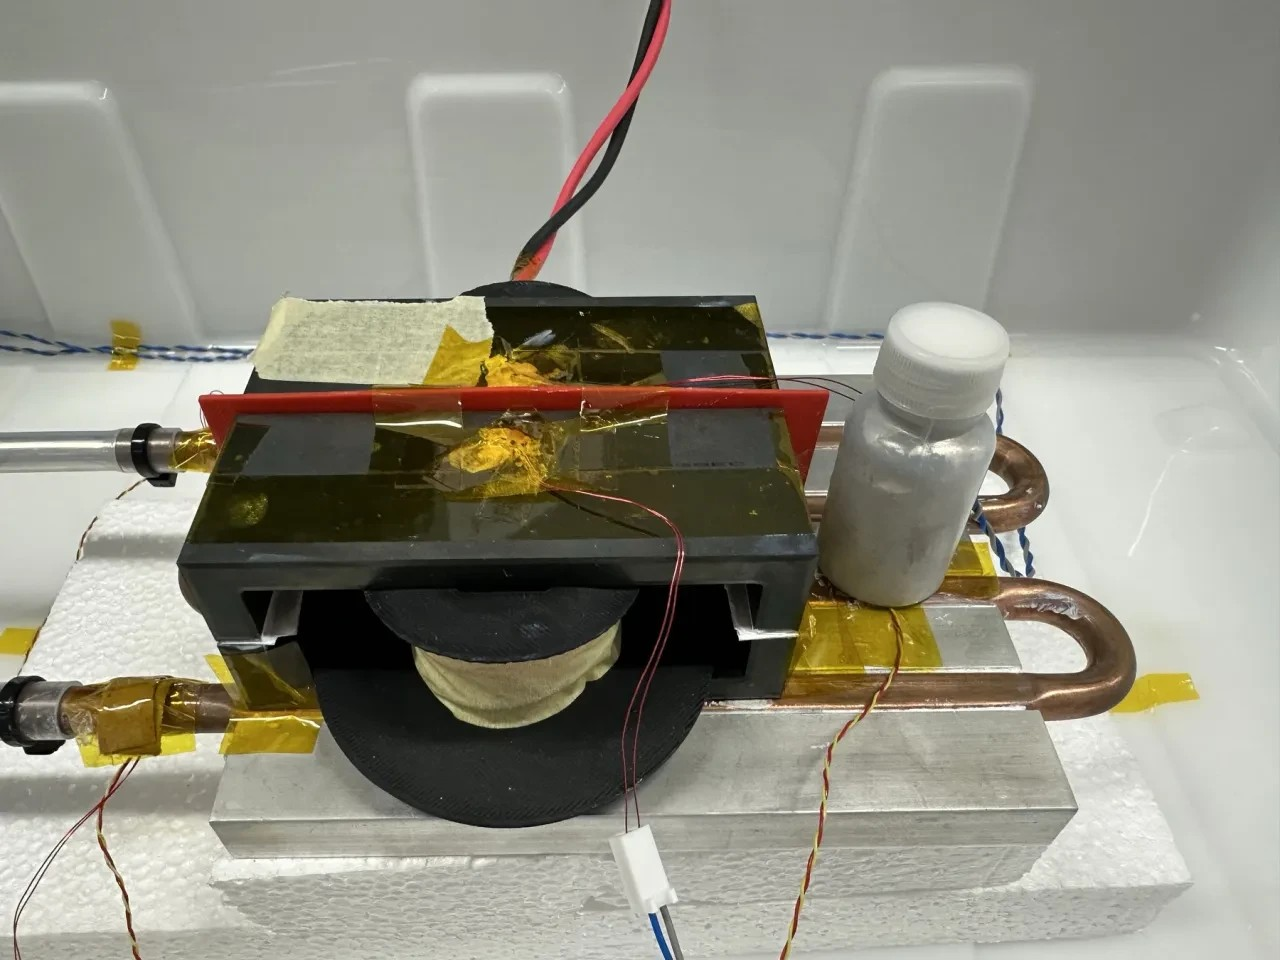
\includegraphics[width=0.6\linewidth]{inductor_vial_setup}
  \caption{Inductor on the Galinstan cold plate, with the PVC vial of Galinstan
    standing beside it, as used for configuration~(iv) of the eddy-current loss
    measurement.}
  \label{fig:vial-setup}
\end{figure}

% =====================================================================
%  Chapter 4 --   Results
% =====================================================================

\chapter{Results}
\label{ch:results}

\subsection{Analytical Thermal Models}

Table~\ref{tab:tn_results} compares the measured and predicted resistor
temperature $T_\mathrm{M}$ and coolant outlet temperature $T_\mathrm{out}$.
$R_\mathrm{pack}$ was calibrated on the two turbulent water tests, so those rows
check the method's consistency rather than validate it independently. Likewise,
Galinstan $T_\mathrm{out}$ is computed from the energy-balance flow rate and
agrees closely by construction. The independent test of the model is therefore
$T_\mathrm{M}$ in the Galinstan and laminar water tests.

\begin{table}[htbp]
    \centering
    \caption{Measured and predicted temperatures
        ($R_\mathrm{pack} = \SI{0.242}{\celsius\per\watt}$; turbulent water
        $R_\mathrm{cp}$ from the ATS datasheet, laminar water from the
        $\varepsilon$-NTU model). $\dagger$~Calibration tests. Galinstan
        $T_\mathrm{out}$ uses the energy-balance flow, so it agrees by construction.}
    \label{tab:tn_results}
    \begin{tabular}{lcccc}
        \toprule
        Test & \multicolumn{2}{c}{$T_\mathrm{M}$ (\si{\celsius})}
             & \multicolumn{2}{c}{$T_\mathrm{out}$ (\si{\celsius})} \\
        \cmidrule(lr){2-3}\cmidrule(lr){4-5}
             & Measured & Predicted & Measured & Predicted \\
        \midrule
        Galinstan \SI{1.4}{\milli\litre\per\second}               & 59.3 & 61.8 & 47.6 & 47.4 \\
        Galinstan \SI{0.75}{\milli\litre\per\second} (\SI{40}{\watt}) & 51.1 & 51.1 & 43.6 & 43.6 \\
        Water \SI{3.6}{\litre\per\minute}$^\dagger$               & 49.2 & 49.3 & 33.5 & 33.4 \\
        Water \SI{1.8}{\litre\per\minute}$^\dagger$               & 48.6 & 48.6 & 32.7 & 32.5 \\
        Water \SI{0.73}{\litre\per\minute}                        & 50.1 & 53.1 & 33.3 & 34.9 \\
        Water \SI{0.5}{\litre\per\minute}                         & 50.5 & 54.1 & 33.9 & 35.7 \\
        \bottomrule
    \end{tabular}
\end{table}

The predicted $T_\mathrm{M}$ lies within the $\pm\SI{3.1}{\celsius}$ measurement
band in five of the six tests, with an RMS error of \SI{1.8}{\celsius} for
Galinstan and \SI{2.3}{\celsius} for water. The turbulent water tests agree
within \SI{0.1}{\celsius}. The mid-flow Galinstan test
(\SI{1.0}{\milli\litre\per\second}) is excluded because its energy balance
closed at only about \SI{80}{\percent}, which indicates a flow-measurement error
or an incomplete approach to steady state.

The two laminar water tests are over-predicted by \SI{3.0}{\celsius} and
\SI{3.6}{\celsius}. In the laminar regime the model's $R_\mathrm{cp}$ rises to
\SIrange{0.074}{0.088}{\celsius\per\watt}, three to four times the turbulent
value. The measurements show no such loss: $T_\mathrm{M} - T_\mathrm{in}$ stays
between \SI{16.1}{\celsius} and \SI{16.6}{\celsius} from
\SIrange{3.6}{0.5}{\litre\per\minute}, and the measured $R_\mathrm{cp}$ follows
the manufacturer's turbulent trend (Figure~\ref{fig:flow_sweep}). This suggests
the flow in these tests was not fully laminar. The flow meter is uncertain below
\SI{1}{\litre\per\minute}, and the Reynolds number scales with
$\dot{V}/\mu$. With $\mu \approx \SI{0.75}{\milli\pascal\second}$ at the
\SI{33}{\celsius} test temperature, the \SI{0.73}{\litre\per\minute} test
reaches $\mathrm{Re} \approx 2600$, inside the transitional range, and any
under-reading of the flow would raise this further. Disturbances from the inlet
and U-bends can also persist at $\mathrm{Re} \approx$ 1300--1900, where the
development length of 66--97 tube diameters far exceeds the 19-diameter pass
length. If these tests are treated as turbulent, the datasheet trend predicts
$T_\mathrm{M}$ within \SI{0.7}{\celsius}. The laminar prediction is therefore
best read as a conservative upper bound. In the turbulent range the
$\varepsilon$-NTU model lies within \SI{15}{\percent} of the datasheet
(\SI{0.024}{\celsius\per\watt} against \SI{0.021}{\celsius\per\watt} at
\SI{2}{\litre\per\minute}).

Galinstan is caloric-limited at every tested flow: at least \SI{97}{\percent} of
its cold-plate resistance is $R_\mathrm{cal}$, so the pump, not the cold-plate
geometry, sets its thermal performance. Hodes et al.~\cite{hodes2014} reached
the same conclusion. Galinstan's volumetric heat capacity is 0.45 times that of
water, and caloric resistance made up \SI{55}{\percent} of the total for their
optimised Galinstan minichannel against \SI{40}{\percent} for water. The larger
share found here reflects a flow rate far below their optimum, and it means
higher pump flow, not improved convection, is the main route to better
liquid-metal performance in this system.
% =====================================================================
%  Chapter 5 -- Discussion
%  Structure follows Kwon (2025): interpretation of results, validity and
%  limitations, relevance to the field.
% =====================================================================
\chapter{Discussion}
\label{sec:discussion}

This chapter interprets the results of \cref{ch:results} against the two
research questions. The thermal performance and pumping power of the Galinstan
loop are discussed first (RQ1), followed by the inductor experiment (RQ2). The
validity and limitations of the measurements and models are then considered,
and finally the relevance of the findings to the cooling of PECs.

% ---------------------------------------------------------------------
\section{Interpretation of Results}
\label{sec:disc-interpretation}

\subsection{Thermal Performance of Galinstan in the Tested Cold Plate}
\label{sec:disc-performance}

The results in \cref{sec:results-measured} show that, at the flow rates
achieved, the Galinstan loop cooled the resistors less effectively than the
water loop, with a total thermal resistance 1.8 to 3.1 times higher
(\cref{tab:measured-performance}). However, the Galinstan tests ran at
\SIrange{0.8}{1.5}{\milli\litre\per\second}, one to two orders of magnitude below
the water tests (\SIrange{8.3}{58.3}{\milli\litre\per\second}). The comparison
therefore reflects the flow the MHD pump could deliver rather than a general
disadvantage of Galinstan as a coolant.

The reason lies in the limiting regime of the cold plate. Galinstan's NTU was 35
to 65 in the tests, so $\varepsilon \approx 1$ and $\Rcp \approx 1/(\mdot\,\cp)$.
The coolant therefore leaves the plate at almost the plate temperature, and heat
removal is limited by the ability of the flow to store and transport heat.
Galinstan's high thermal conductivity gives a wall heat transfer coefficient of
about \SI{7700}{\watt\per\metre\squared\per\kelvin}, roughly 7.5 times that of
laminar water (\cref{app:convection}). Its convective resistance $1/(hA)$ of
\SI{0.0085}{\celsius\per\watt} is lower than that of water even in turbulent
flow (\SIrange{0.012}{0.023}{\celsius\per\watt}). This advantage, however, is
not used in the current setup, because the convective term accounts for less
than \SI{3}{\percent} of Galinstan's $\Rcp$. Water, by contrast, has
$\NTU \approx 0.3$--0.4 at every tested flow, so convection makes up about
\SI{85}{\percent} of its $\Rcp$. These results support H1: Galinstan lowers the
convective resistance, but its low volumetric heat capacity and low flow rate
give a caloric resistance at least as large as the package resistance, so the
total resistance of the Galinstan loop is higher than that of the water loop.

\Cref{fig:disc-regimes}(a) extends this analysis over the full flow range.
Galinstan remains caloric-limited ($\NTU > 3$) over the whole laminar range and
up to about \SI{50}{\milli\litre\per\second}. Water, in contrast, stays close to
the convection-limited boundary above about \SI{10}{\milli\litre\per\second}.
For a caloric-limited coolant, the most important property is the volumetric
heat capacity $\rho\cp$, and here water has the advantage
(\cref{tab:disc-properties}): it absorbs about 1.8 times more heat per unit
volume per degree.

The same behaviour gives the Galinstan loop a much larger actuation range.
Because its cold plate is caloric-limited, its resistance follows the flow:
roughly halving the Galinstan flow, from 1.45 to
\SI{0.77}{\milli\litre\per\second}, raised the total resistance from 0.488 to
\SI{0.799}{\celsius\per\watt} (\cref{tab:measured-performance}). The
convection-limited water plate, in contrast, barely responded, with the total
resistance changing only from 0.257 to \SI{0.267}{\celsius\per\watt} over a
seven-fold change in flow. As discussed in \cref{sec:reliability}, the
flow rate of a single-phase loop is the control input used to suppress the
temperature swing of a component, part of the reliability requirement for PEC
thermal management (\cref{tab:cooling-strategies}). The pressure of an MHD pump
scales directly with its current (\cref{sec:em-pumping}), so the Galinstan loop
offers direct control over the component temperature through the pump current
across a wide range. In the tested water loop, changing the flow had almost no
effect on the resistor temperature. This range comes at the cost of a higher
resistance at the flows achieved here, but it is an advantage where the
temperature swing, rather than the peak temperature, limits component lifetime.

\begin{table}[htbp]
  \centering
  \caption{Coolant properties relevant to suitability. Thermal properties are
    those used in the model (\cref{tab:coolant-properties}).}
  \label{tab:disc-properties}
  \small
  \begin{tabularx}{\linewidth}{@{}lrrX@{}}
    \toprule
    Property & Galinstan & Water & Implication \\
    \midrule
    $\rho\cp$ (\si{\mega\joule\per\metre\cubed\per\kelvin})
      & 2.33 & 4.18 & Water carries 1.8$\times$ more heat per unit flow \\
    $k$ (\si{\watt\per\metre\per\kelvin}) & 16.5 & 0.60
      & Galinstan $h$ is about 27$\times$ higher at equal Nu \\
    $\mu$ (\si{\milli\pascal\second}) & 2.4 & 1.0
      & Laminar pressure drop 2.4$\times$ higher at equal flow \\
    $\rho$ (\si{\kilogram\per\metre\cubed}) & 6370 & 1000
      & 6.4$\times$ coolant mass for the same volume \\
    Pr & 0.053 & 6.97 & Heat diffuses far faster than momentum in Galinstan \\
    Electrical conductivity (\si{\siemens\per\metre})
      & $3.46 \times 10^{6}$~\cite{noauthor_gainsn_nodate} & $\ll 1$
      & Galinstan can be pumped electromagnetically, but heats and is retarded
        in AC fields \\
    Liquid range at \SI{1}{atm} (\si{\celsius})
      & 10 to $>1300$~\cite{noauthor_gainsn_nodate,hodes_potential_2014}
      & 0 to 100 & Galinstan cannot boil at component temperatures \\
    \bottomrule
  \end{tabularx}
\end{table}
\edited{\Cref{tab:disc-properties}: citations added for the electrical
conductivity and liquid range, matching \cref{tab:galinstan-properties}. The
lower end of the liquid range was $-19$; it is now \SI{10}{\celsius}, the
melting point of the grade used in this work (\cref{tab:galinstan-properties}).}

\begin{figure}[htbp]
  \centering
  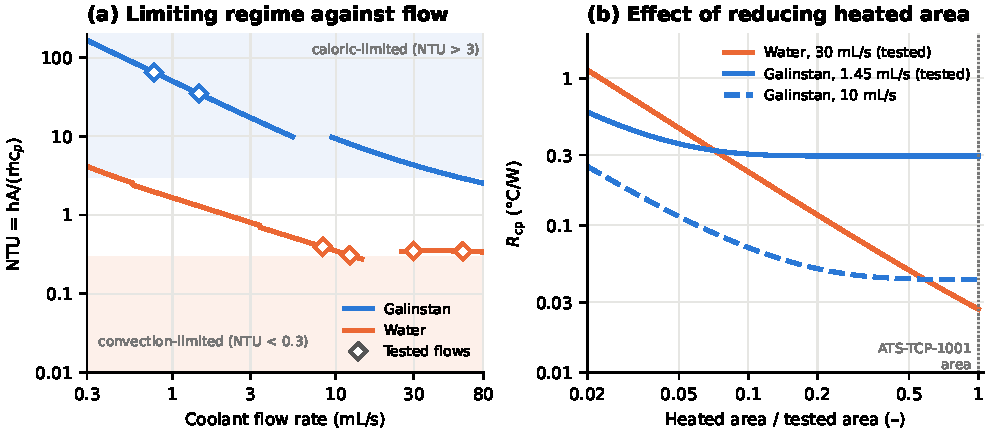
\includegraphics[width=\textwidth]{discussion_regimes.pdf}
  \caption{(a) NTU against flow rate for both coolants in the ATS-TCP-1001 cold
    plate, with the tested flows marked. Galinstan remains caloric-limited over
    the laminar range; water sits near the convection-limited boundary. Gaps
    mark the transitional range ($2300 < \mathrm{Re} < 4000$); turbulent
    Galinstan uses the Seban--Shimazaki correlation~\cite{bergman_fundamentals_2017}.
    (b) Indicative effect of reducing the heated area at fixed flow, with $h$
    held at its tested-geometry value. Water's $\Rcp$ rises in proportion to
    $1/A$, while Galinstan's at the tested flow is almost unaffected until the
    area falls to about a tenth of the tested value.}
  \label{fig:disc-regimes}
\end{figure}

\subsection{Pumping Power and Scalability}
\label{sec:disc-pumping}

RQ1 also asks how the pumping power of the two loops compares. At full flow, the
MHD pump drew \SI{0.85}{\watt}, about \SI{7}{\percent} of the \SI{11.5}{\watt}
drawn by the water pump, and it was more than 50 times smaller
(\cref{tab:pumps}). This is in line with An \emph{et al.}, who found that a
conduction pump drew less than \SI{15}{\percent} of the power of a mechanical
water pump for the same cooling performance~\cite{an_liquid_2024}, although here
the Galinstan loop also cooled less effectively. Per watt of pump power, the
Galinstan loop handled more heat, with a maximum coefficient of performance
(COP) of 200 against 47.6 for water. The low power draw does not, however,
reflect an efficient pump. The maximum mechanical efficiency of the MHD pump,
\SI{0.56}{\percent},
is an order of magnitude below the \SIrange{6}{10}{\percent} reported for DC
conduction pumps~\cite{an_liquid_2024,hodes_potential_2014}
(\cref{sec:em-pumping}), and far below the \SI{28.7}{\percent} of the
centrifugal water pump. Almost all of its input power is therefore dissipated
rather than delivered to the flow, which leaves considerable scope for a
redesigned pump. Fan \emph{et al.} show what is achievable: by reducing the
pressure drop of their loops to about one sixth with optimised connections and
cold plates, their MHD pumps reached flows of up to about
\SI{10}{\milli\litre\per\second} for less than
\SI{0.1}{\watt}~\cite{fan_liquid_2021,fan_high_2023} (\cref{tab:fan-comparison}). It is worth noting that the MHD pump was already at the
\SI{18}{\ampere} limit of its supply at full flow, so the Galinstan loop could
not be run at a higher flow.

For scalability, the more important question is the flow Galinstan would need
to match water. Because the cold plate is caloric-limited, the Galinstan $\Rcp$
is almost inversely proportional to the flow rate, as the simulations confirm up
to \SI{5}{\milli\litre\per\second} (\cref{fig:galinstan_rcp_cfd}). To match the
heat-capacity rate of
water at \SI{29.2}{\milli\litre\per\second} (\SI{122.0}{\watt\per\kelvin}),
Galinstan would need about \SI{52}{\milli\litre\per\second}, around 36 times the
full flow achieved here. The pressure of a DC conduction pump scales with current,
as shown by \cref{eq:mhd-pressure}, and the existing pump delivered
\SI{1.4}{\milli\litre\per\second} at the \SI{18}{\ampere} limit of its supply.
An increase in flow of this size would therefore require a redesigned pump
rather than simply a higher current. At equal volumetric flow, Galinstan also
needs about 2.4 times the pressure of water in laminar flow because of its higher
viscosity, and its density is 6.4 times that of water, which adds weight to the
loop (\cref{tab:disc-properties}). A comparison at equal pumping power, rather
than at the flow each pump could deliver, would therefore penalise Galinstan
further.

\subsection{Inductor Cooling and Eddy-Current Loss}
\label{sec:disc-inductor}

RQ2 asks whether the Galinstan loop can cool a power-dense inductor while adding
minimal loss, and how large the eddy-current loss induced in the coolant is. The
inductor was operated at an estimated loss of \SI{42.76}{\watt}, more than twice
the \SI{17.88}{\watt} datasheet loss limit above which its core requires active
cooling (\cref{sec:analytical-design}). Its maximum surface temperature was about
\SI{83}{\celsius} (\cref{fig:inductor-cam}), which shows that the Galinstan
loop can cool a power-dense inductor operating well beyond the loss its core
can dissipate without active cooling. The cooling effect of the plate is clear
from the steady-state thermal images: the upper core, which relies on natural
convection, ran markedly hotter than the lower core, which sits on the cold
plate (\cref{fig:inductor-cam-a}). This supports the first part of H2, that the
Galinstan loop cools the inductor beyond natural convection. The same difference
shows that the single-sided cold plate leaves part of the inductor's loss to be
removed by convection, and cooling both cores, as in the inductor of Gao
\emph{et al.}~\cite{gao_modeling_2022}, would make better use of the coolant.

The eddy-current measurements support the second part of H2. Placing the
inductor on the cold plate added \SI{11.7}{\milli\ohm} to the winding
resistance, whereas filling the plate with Galinstan added only
\SI{1.0}{\milli\ohm}, less than a tenth of the plate's own contribution. As
argued in H2,
the metal of the cold plate between the inductor and the
coolant is several skin depths thick at \SI{85}{\kilo\hertz}, so it shields the
Galinstan from the leakage field. Unshielded Galinstan is far more exposed: its
own skin depth at this frequency is about \SI{0.9}{\milli\metre} (for
$\sigma = \SI{3.46e6}{\siemens\per\metre}$~\cite{noauthor_gainsn_nodate}),
comparable to practical channel dimensions. The vial of Galinstan outside the
plate added \SI{10.3}{\milli\ohm}, an order of magnitude more than the coolant
inside the plate, although its volume and position differ. This agrees with the
initial ANSYS simulation, which found that \SI{1}{\milli\metre} of copper
shielding reduced the eddy-current loss in the coolant by more than
\SI{70}{\percent} (\cref{sec:inductor-design}). Without the plate, the effect of
the vial also fell with distance, from \SI{9.0}{\milli\ohm} at
\SI{1}{\centi\metre} to \SI{2.15}{\milli\ohm} beyond \SI{4}{\centi\metre}
(\cref{fig:rac_distance}), so keeping unshielded coolant a few centimetres from
the magnetics also limits the loss. Finally, the coolant flow did not change
measurably when the inductor was energised, which supports the final part of
H2.

% ---------------------------------------------------------------------
\section{Validity and Limitations}
\label{sec:disc-validity}

The steady-state data collected in this study are consistent across the two
loops and with the thermal models, but the conclusions rest on two Galinstan
tests and four water tests, and their limitations should be weighed. Four points
stand out.

First, the low-flow water results are limited by the flow measurement rather
than by the model. The measured $\Tres - \Tin$ stays between
\SI{16.1}{\celsius} and \SI{16.6}{\celsius} from
\SIrange{58.3}{8.3}{\milli\litre\per\second}, and the measured $\Rcp$ of
\SI{0.025}{\celsius\per\watt} at \SI{0.5}{\litre\per\minute} lies below water's
caloric limit $1/(\mdot\,\cp)$ of \SI{0.029}{\celsius\per\watt} at the indicated
flow (\cref{fig:water_rcp}). A cold plate cannot have $\Rcp < 1/(\mdot\,\cp)$, so
the true flow in that test must have been at least
\SI{9.6}{\milli\litre\per\second}, about \SI{15}{\percent} above the reading.
This supports the conclusion that the flow meter under-reads below its rated
range. It is also likely that these tests were not truly laminar. With the water
viscosity of about \SI{0.75}{\milli\pascal\second} at the \SI{33}{\celsius} test
temperature, the \SI{0.73}{\litre\per\minute} test reaches
$\mathrm{Re} \approx 2600$, in the transitional range, and any under-reading of
the flow raises this further. Disturbances from the pump, the valve and the
U-bends can also persist in the short passes, where the thermal entry length far
exceeds the pass length. If these tests are treated as turbulent, the datasheet
trend predicts $\Tres$ within \SI{0.7}{\celsius}, so the laminar
predictions in \cref{tab:tn_results} are best read as a conservative upper
bound.

Second, $\Rpack$ was calibrated on the turbulent water tests, where the plate is
close to isothermal. Galinstan's coolant temperature rise of
\SIrange{17}{18}{\celsius} violates this assumption: the outlet end of the plate
runs hotter than the mean, and the $\Rpack$ inferred for Galinstan ranges from
\SIrange{0.19}{0.24}{\celsius\per\watt} for an isothermal plate to
\SIrange{0.33}{0.51}{\celsius\per\watt} for uniform heat flux. The full-flow
Galinstan point lying slightly below its caloric limit (\cref{fig:galinstan_rcp})
is consistent with this. The Galinstan flow itself also relies on a small EMF,
which is less accurate at lower pump current, although it agreed with the energy
balance to within \SI{4}{\percent}. The lumped model therefore describes
Galinstan less reliably than water, although its prediction of the Galinstan
resistor temperatures to within \SI{2.5}{\celsius} (\cref{sec:results-tn})
shows that it captures the dominant behaviour.

Third, the conjugate heat transfer simulations address the main weakness of the
lumped model. They are mesh-independent above \num{427e3} cells and reproduce
all four probe temperatures within \SI{1.4}{\celsius} for both Galinstan tests.
The consistent over-prediction of the right-hand resistor by about
\SI{1.3}{\celsius} in both runs suggests a small systematic asymmetry in the
model, such as the heat-load distribution, rather than random error. For water,
the model under-predicts the resistor temperatures by about
\SIrange{2.3}{2.4}{\celsius}, which points to an over-predicted wall heat
transfer coefficient in the turbulent model (\cref{app:cht_validation}). The
model is therefore slightly pessimistic for Galinstan and optimistic for water,
so any advantage it shows for Galinstan is, if anything, understated. With this
in mind, the CHT model can be used with reasonable confidence to compare
geometries and flows that the test rig could not reach.

Fourth, the inductor experiment was run at a single operating point. Its heat
load is an estimate from the core-loss model and the measured winding
resistance, and the measured surface temperature of about \SI{83}{\celsius} is
above the \SI{65}{\celsius} assumed when the core loss was modelled, so the true
core loss will differ from the \SI{30.81}{\watt} estimate. The AC resistances
in \cref{fig:rac_configurations,fig:rac_distance} were measured at the
\SI{85}{\kilo\hertz} operating frequency, but each value comes from a single
measurement at low excitation, and the absolute resistance varied between
sessions, so only changes within a session are compared.

More generally, the study used a single cold plate designed for water, and the
coolants were compared at the flow each pump could deliver rather than at equal
pumping power. The water temperature rise across the plate was also below the
thermocouple accuracy, so the water energy balance could not be checked
independently.

% ---------------------------------------------------------------------
\section{Relevance to the Field}
\label{sec:disc-suitability}

The NTU analysis gives a clear criterion for where Galinstan is advantageous:
where the cooling surface, rather than the coolant flow, limits heat removal,
that is, where water would be convection-limited. \Cref{fig:disc-regimes}(b)
illustrates this using the $\varepsilon$--NTU model. The heated area is scaled
by a factor $f$ while the flow rate and heat transfer coefficient are held at
their values in the tested cold plate, so that $\NTU$ falls in proportion to $f$
and $\Rcp = 1/[\mdot\,\cp\,(1 - e^{-f\,\NTU_0})]$, where $\NTU_0$ is the value
for the full plate. This represents concentrating the same heat into a smaller
footprint or a shorter heated length, and the method and its assumptions are
given in \cref{app:area-scaling}. Reducing the heated area at fixed flow raises
water's $\Rcp$ almost in proportion, because water is already close to
convection-limited. At the tested flow, Galinstan's $\Rcp$ barely changes until
the area is reduced to about a tenth, because it simply uses up its excess
$hA$. At \SI{5}{\percent} of the tested area, Galinstan at
\SI{10}{\milli\litre\per\second} ($\Rcp \approx \SI{0.12}{\celsius\per\watt}$)
outperforms water at three times the flow
($\Rcp \approx \SI{0.46}{\celsius\per\watt}$). Galinstan's resistance only
begins to rise once $f\,\NTU_0$ falls to about 3, so a coolant that starts with a
large NTU can absorb a large reduction in area before its performance suffers.
Because $h$ is held fixed and pressure drop is not considered, the result is
indicative only, but it shows the type of application in which Galinstan's
conductivity becomes useful.
\edited{``About a fifth'' changed to ``about a tenth'': with $\NTU_0 = 34.9$ the
resistance starts to rise at $f \approx 3/\NTU_0 = 0.09$ (\cref{app:area-scaling}),
and \cref{tab:app-area} shows no change at $f = 0.2$. The caption of
\cref{fig:disc-regimes} was changed to match.}

Galinstan is therefore best suited to applications that combine (i)~high heat
flux over a small area, such as direct cooling of power semiconductors or local
hot spots, or minichannel and microchannel heat sinks; (ii)~a pump able to
deliver flow rates comparable to water, for which a sealed electromagnetic pump
with no moving parts may offer a reliability advantage; (iii)~component
temperatures near or above \SI{100}{\celsius}, where water would boil without
pressurisation; and (iv)~locations away from strong alternating magnetic fields,
or where the coolant is shielded from them by the cold plate, as in
\cref{sec:disc-inductor}.

In an IPT system, these criteria point to the power electronics, rather than the
pads, as the best place for Galinstan. In the \SI{10}{\kilo\watt} system of Kim
\emph{et al.}, the inverter and rectifier each dissipated about
\SIrange{70}{80}{\watt} in small switching devices placed away from the coupler,
where the heat flux is high and the magnetic field is weak
(\cref{sec:ipt-losses})~\cite{kim_thermal_2022}. The larger pad losses, by
contrast, are spread over about \SI{0.5}{\metre\squared} inside the strongest
alternating field at \SI{85}{\kilo\hertz}, so a cold plate under the pad would
see a low heat flux, for which water is adequate, together with a strong leakage
field. The inductor experiment shows that the leakage field need not rule
Galinstan out: coolant shielded by the metal of the cold plate added only
\SI{1.0}{\milli\ohm} to the winding resistance at \SI{85}{\kilo\hertz}, against
\SI{10.3}{\milli\ohm} for unshielded coolant beside the inductor
(\cref{sec:results-eddy}). Galinstan could therefore also cool compact
magnetics, such as the tank inductors and transformer, where heat is
concentrated in a small volume, provided the coolant is shielded.
\Cref{tab:disc-suitability} applies these criteria to the main components of an
IPT system.

\begin{table}[htbp]
  \centering
  \caption{Indicative suitability of Galinstan cooling for IPT system
    components, based on the criteria of \cref{sec:disc-suitability}.}
  \label{tab:disc-suitability}
  \small
  \begin{tabularx}{\linewidth}{@{}l>{\raggedright\arraybackslash}p{2.6cm}cX@{}}
    \toprule
    Component & Heat load character & Suitability & Reason \\
    \midrule
    Inverter and rectifier modules & High flux, small area & Good
      & Water likely convection-limited; much weaker AC fields than at the
        coupler \\
    Compact magnetics (tank inductors, transformer) & High flux, small volume
      & Possible
      & Leakage-field loss is small if the coolant is shielded by the cold
        plate (\cref{sec:results-eddy}) \\
    Coupler coils (Litz) and ferrite pads & Distributed, low flux & Limited
      & Large area, where water is adequate; strongest AC field, so the coolant
        must be shielded \\
    Resonant compensation capacitors & Moderate flux & Limited
      & Benefit only if close to their temperature limit; proximity to high
        voltage and AC fields \\
    Vehicle-side assembly & Weight-sensitive & Poor
      & 6.4$\times$ the coolant mass of water, and high material cost \\
    Large cold plates at low flow (as tested) & Low flux, large area & Poor
      & Caloric-limited; water carries 1.8$\times$ more heat per unit flow \\
    \bottomrule
  \end{tabularx}
\end{table}
\edited{\Cref{tab:disc-suitability}: coupler coils and pads changed from
``Poor'' to ``Limited'', since the eddy-current results show that a shielding
cold plate keeps the coolant's loss small, and a row added for compact magnetics,
which the inductor experiment represents.}

These findings agree with Hodes \emph{et al.}~\cite{hodes_potential_2014}, who
found that Galinstan's low volumetric heat capacity makes its caloric resistance
a larger share of the total than for water (\SI{55}{\percent} against
\SI{40}{\percent} in their optimised minichannel), and that its advantage depends
on geometries that exploit its high conductivity. The larger caloric share found
here (above \SI{97}{\percent}) reflects a cold plate designed for water and a
flow rate far below their optimum, rather than a contradiction of their result.
\issue{Check the volumetric heat-capacity ratio: Hodes quote 0.45, while the
properties used here give $2.33/4.18 = 0.56$; the difference is likely the
Galinstan $\cp$ (see the 360 vs \SI{366}{\joule\per\kilogram\per\kelvin} note).
\Cref{tab:galinstan-properties} also quotes 0.45.}

Despite the limitations above, the results show that a magnetohydrodynamically
pumped Galinstan loop can cool both a resistive load and a power-dense inductor,
and that the loss it adds near magnetics can be kept small when the coolant is
shielded by the cold plate. Its performance in the tested system is set by the
pump rather than by the coolant, so the case for liquid metal cooling in PECs
rests on higher-flow pumps and on cold plates designed to exploit its high
conductivity.

% ---------------------------------------------------------------------
\section{Recommendations for Further Work}
\label{sec:disc-limitations}

Further work should:
\begin{enumerate}
  \item compare the coolants at equal pumping power, using the CHT model to
    obtain the pressure drop as well as the temperature;
  \item test Galinstan at higher flow rates, closer to
    \SIrange{10}{30}{\milli\litre\per\second}, with an independently calibrated
    flow meter, which will require a redesigned pump;
  \item use the CHT model to evaluate small-area, high-flux geometries such as
    minichannel cold plates, where \cref{fig:disc-regimes}(b) indicates that
    Galinstan may outperform water;
  \item repeat the inductor test with the pump off and with the coolant
    unshielded, repeat the $R_{\mathrm{ac}}$ measurements to estimate their
    spread, and quantify eddy-current heating and MHD drag through coupled
    electromagnetic--thermal analysis before Galinstan is placed near an IPT
    coupler; and
  \item assess long-term material compatibility, since gallium alloys attack
    aluminium and copper requires protection at higher
    temperatures~\cite{an_liquid_2024}.
\end{enumerate}

% =====================================================================
%  Chapter 6 -- Conclusion
% =====================================================================
\chapter{Conclusion}
\label{ch:conclusion}

As PECs become more power-dense, removing their losses from a smaller volume
increasingly limits their design. This project evaluated MHD-pumped Galinstan as
a coolant for such converters, and identified where in an IPT system it is most
useful. A Galinstan loop and a water loop were compared on the same commercial
cold plate under resistive heat loads, the results were interpreted with an
$\varepsilon$--NTU thermal network and extended with a validated conjugate heat
transfer simulation, and the Galinstan loop was used to cool a power-dense
\SI{85}{\kilo\hertz} planar inductor.

\textbf{RQ1.} At the flows each pump could deliver, water outperformed
Galinstan, with a total resistance from the resistor to the coolant inlet of
\SIrange{0.257}{0.267}{\celsius\per\watt} against
\SIrange{0.488}{0.799}{\celsius\per\watt}. The $\varepsilon$--NTU analysis
explains this result and supports H1. Galinstan's high thermal conductivity
reduced its convective resistance to less than \SI{3}{\percent} of the cold-plate
resistance, but at \SIrange{0.77}{1.45}{\milli\litre\per\second} the plate was
caloric-limited, so Galinstan's low volumetric heat capacity set its
performance. The water plate, in contrast, was convection-limited and barely
responded to a seven-fold change in flow. The MHD pump drew only
\SI{0.85}{\watt}, against \SI{11.5}{\watt} for the water pump, giving a maximum
COP of 200 against 47.6, but its mechanical efficiency was only
\SI{0.56}{\percent}. The simulation shows that at
\SI{5}{\milli\litre\per\second}, the limit of laminar flow, the Galinstan total
resistance would fall to about \SI{0.29}{\celsius\per\watt}, within
\SI{14}{\percent} of water at a lower flow than any of the water tests.

\textbf{RQ2.} The Galinstan loop cooled the inductor, running at more than twice
the loss its core can dissipate without active cooling, to a maximum surface
temperature of about \SI{83}{\celsius}. Galinstan inside the cold plate added
only \SI{1.0}{\milli\ohm} to the winding AC resistance at
\SI{85}{\kilo\hertz}, against \SI{11.7}{\milli\ohm} for the plate itself and
\SI{10.3}{\milli\ohm} for unshielded Galinstan beside the inductor. The metal of
the cold plate therefore shields the coolant from the leakage field, supporting
H2, although the effect of the field on the flow could not be confirmed.

The main contribution of this work is to show when Galinstan is worth using.
Its advantage lies not in its conductivity alone, but in applications where the
heated area is small and the heat flux high: at \SI{5}{\milli\litre\per\second},
the model predicts that it outperforms water once the heated area falls below
about \SI{40}{\centi\metre\squared}. In an IPT system, this points to the
inverter and rectifier modules and to shielded compact magnetics, rather than
the large, distributed losses of the pads. These conclusions rest on a small
number of tests on a single cold plate designed for water, and the area
analysis is indicative only. Realising Galinstan's advantage will require a more
efficient, higher-flow pump with integrated power electronics, and a smaller cold
plate designed for liquid metal (\cref{sec:disc-further-work}).


%\backmatter
%\printbibliography[heading=bibintoc,title={References}]

%\appendix
% cleveref does not detect \appendix here, so appendix chapters were cited as
% "Chapter A". Label them (and their sections) as appendices explicitly; the
% names are set with the other \crefname commands in the preamble.
%\crefalias{chapter}{appendix}
%\crefalias{section}{subappendix}
%% =====================================================================
% Appendix: Validation of the SimScale conjugate heat transfer model
% Requires: graphicx, subcaption, siunitx (v2 \SI syntax, as in main report)
% =====================================================================

\chapter{Conjugate Heat Transfer Model}
\label{app:cht_validation}

The SimScale conjugate heat transfer (CHT) model was checked in three stages
before its results were used: a mesh independence study to bound the
discretisation error, a check of iterative convergence, and a comparison of the
converged probe temperatures against the experimental measurements. The
acceptance criterion throughout was the $\pm\SI{2.2}{\celsius}$ tolerance of the
thermocouples. Numerical errors well inside this band can be neglected, so any
remaining disagreement with experiment can be attributed to the modelling
assumptions or to the measurements themselves.

\subsubsection{Flow Regime and Mesh Independence}

Turbulent cases were solved with the $k$--$\omega$ SST turbulence model, and a
laminar model was used for runs with an estimated $\mathrm{Re} \leq 2110$.
Because the two models resolve the near-wall region differently, mesh
independence was assessed separately for each flow regime and each coolant.
Each study was performed at the most demanding operating point in its regime,
the highest flow rate, where the boundary layers are thinnest and the near-wall
gradients steepest. A mesh that resolves this case is therefore conservative for
the lower flow rates in the same regime. Separate studies were needed for the
two coolants because their Prandtl numbers differ by more than two orders of
magnitude. Galinstan ($\mathrm{Pr} \sim 10^{-2}$) develops a thermal boundary
layer much thicker than its velocity boundary layer, whereas water
($\mathrm{Pr} \approx 5$--$7$) has a thermal boundary layer thinner than its
velocity boundary layer and so needs finer near-wall resolution to capture the
temperature field. The same sequence of five meshes, from \num{73e3} to
\num{1.5e6} cells, was used in every study.
% NOTE: your earlier paragraph said "three" meshes; the figure shows five.

Figure~\ref{fig:mesh_independence} shows the study for Galinstan at
\SI{1.4}{\milli\litre\per\second}. The inlet and outlet temperatures vary by
less than \SI{0.1}{\celsius} across the full range. The inlet is fixed by the
boundary condition and the outlet is set largely by the bulk energy balance, so
neither depends strongly on near-wall resolution. The resistor temperatures are
the sensitive quantities, because they depend on resolving conduction through
the cold plate and the temperature gradient at the wall. The two coarsest
meshes underpredict them by up to \SI{2.75}{\celsius} relative to the finest
mesh, which exceeds the thermocouple tolerance. From \num{427e3} cells upward,
every probe lies within \SI{0.25}{\celsius} of the \num{1.5e6}-cell result.
Convergence is not strictly monotonic: the \num{427e3}- and \num{655e3}-cell
meshes slightly overshoot the finest mesh, and the refinement ratio between
successive meshes is not constant. Richardson extrapolation and the grid
convergence index, which assume monotonic convergence at a fixed refinement
ratio, were therefore not applied. Instead, the \SI{0.25}{\celsius} residual
change was compared directly with the measurement tolerance, and it is about
one ninth of that tolerance. The \num{427e3}-cell mesh was adopted for the
Galinstan simulations because it is the coarsest mesh whose discretisation
error is negligible against the measurement uncertainty.
% CHECK: confirm 427k is the mesh actually used for the reported runs.

\begin{figure}[htbp]
    \centering
    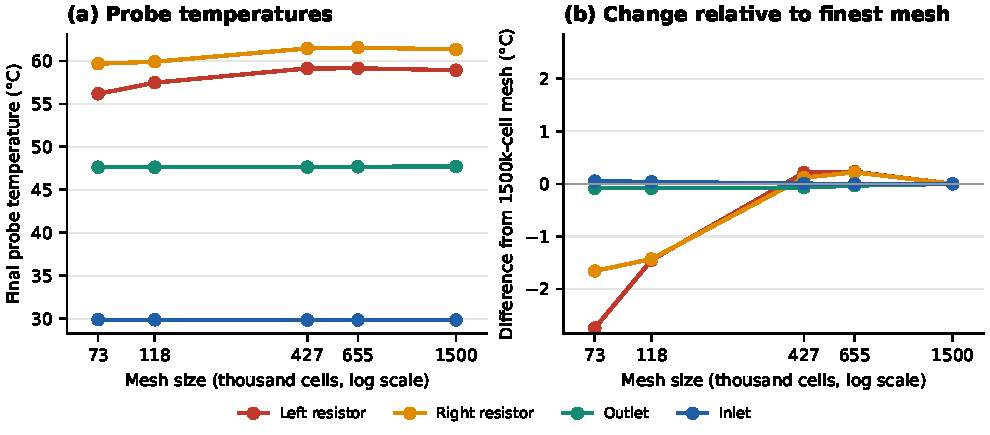
\includegraphics[width=\textwidth]{mesh_independence.pdf}
    \caption{Mesh independence study for Galinstan at
        \SI{1.4}{\milli\litre\per\second}: (a) final probe temperatures and
        (b) change relative to the \num{1.5e6}-cell mesh. All probes change by
        less than \SI{0.25}{\celsius} between \num{427e3} and
        \num{1.5e6} cells.}
    \label{fig:mesh_independence}
\end{figure}

Figure~\ref{fig:mesh_independence_water} shows the corresponding study for
the turbulent water model at \SI{3.6}{\litre\per\minute}. The pattern is the
same: the inlet and outlet vary by less than \SI{0.03}{\celsius}, and the
resistor temperatures are underpredicted on the coarsest meshes, by up to
\SI{2.5}{\celsius} at \num{73e3} cells. The fine meshes settle more slowly than
they do for Galinstan, however. At \num{427e3} cells the resistors still differ
from the \num{1.5e6}-cell result by up to \SI{0.58}{\celsius}, and at
\num{655e3} cells by \SI{0.38}{\celsius}, compared with less than
\SI{0.25}{\celsius} for Galinstan on the same meshes. This is the behaviour the
Prandtl number argument predicts: the thinner thermal boundary layer in water
needs finer near-wall resolution before the wall temperature gradient, and
hence the resistor temperature, stops changing. Above \num{427e3} cells the
resistor temperatures fall monotonically with refinement, so the
\num{1.5e6}-cell result is itself probably still a few tenths of a degree from a
fully mesh-independent value. The \num{427e3}-cell mesh was retained for water.
Its discretisation error of about \SI{0.6}{\celsius} is roughly a quarter of the
thermocouple tolerance: acceptable for comparison with experiment, but not
negligible in the way it is for Galinstan.
% CHECK: confirm which mesh the water runs used. If 655k, replace the last two
% sentences: error about 0.4 C, roughly a sixth of the tolerance.
% NOTE: this is the turbulent water study. If a laminar water study (low flow)
% was also run, it needs its own figure or a sentence here.

\begin{figure}[htbp]
    \centering
    \figureorplaceholder[width=\textwidth]{mesh_independence_water.pdf}
    \caption{Mesh independence study for water at
        \SI{3.6}{\litre\per\minute} ($k$--$\omega$ SST): (a) final probe
        temperatures and (b) change relative to the \num{1.5e6}-cell mesh,
        plotted on the same scale as Figure~\ref{fig:mesh_independence}. The
        inlet and outlet differ by only \SI{0.26}{\celsius} and overlap in (a).
        The resistor temperatures change by up to \SI{0.58}{\celsius} between
        \num{427e3} and \num{1.5e6} cells.}
    \label{fig:mesh_independence_water}
\end{figure}
\issue{The measured full water flow is now \SI{3.5}{\litre\per\minute}
(\SI{58.3}{\milli\litre\per\second}) in the main text. This appendix still says
the water simulations ran at \SI{3.6}{\litre\per\minute}. If that is the flow
set in SimScale, keep it and say so; otherwise change it to
\SI{3.5}{\litre\per\minute}.}

\subsubsection{Iterative Convergence}

The model was solved as a steady-state problem, and convergence was judged by
monitoring the probe temperatures, since these are the quantities compared
against experiment (Figure~\ref{fig:simscale_full}). The inlet temperature
settles within about 150 iterations because it is fixed by the boundary
condition. The outlet and resistor temperatures relax far more slowly, decaying
over several thousand iterations after an initial overshoot. This behaviour is
typical of conjugate heat transfer: heat crosses the solid regions by
conduction alone, so the solid temperature field relaxes much more slowly than
the flow field. By 4000 iterations the outlet temperature had levelled off,
while the resistor temperatures were still falling by about \SI{0.3}{\celsius}
over the final 1000 iterations.
% CHECK: drift read from the plot; confirm from the exported probe data.
The fully converged resistor temperatures would therefore be slightly lower
than those reported. This drift is small relative to the measurement tolerance,
but it is not zero, and its direction matters for the comparison below: it would
move the right resistor towards the measured value and the left resistor
slightly further below it. The water model converges much faster
(Figure~\ref{fig:simscale_water}). After an initial transient, every probe is
within \SI{0.01}{\celsius} of its final value by about 1000 iterations, and at
every mesh density no probe changes by more than \SI{0.001}{\celsius} over the
final 1000 iterations. Iterative error is therefore negligible for water.

\begin{figure}[htbp]
    \centering
    \begin{subfigure}{\textwidth}
        \centering
        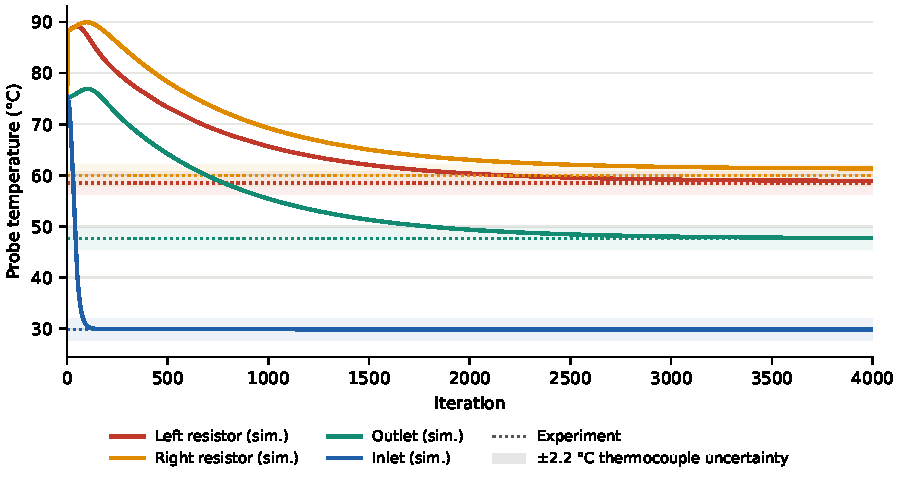
\includegraphics[width=0.9\textwidth]{simscale_convergence_full.pdf}
        \caption{Galinstan, \SI{1.4}{\milli\litre\per\second} (\SI{72}{\watt})}
        \label{fig:simscale_full}
    \end{subfigure}

    \vspace{0.6em}
    \begin{subfigure}{\textwidth}
        \centering
        \figureorplaceholder[width=0.9\textwidth]{simscale_convergence_water.pdf}
        \caption{Water, \SI{3.6}{\litre\per\minute} (\SI{72}{\watt}),
            \num{427e3} cells}
        \label{fig:simscale_water}
    \end{subfigure}
    \caption{Convergence of the SimScale conjugate heat transfer model against
        experiment. Solid lines show the simulated probe temperatures at each
        iteration; dotted lines show the measured values, with shaded bands for
        the $\pm\SI{2.2}{\celsius}$ thermocouple uncertainty. The measured
        resistor value is the mean of the two resistors. For Galinstan all
        probes lie within the measurement uncertainty at the final iteration;
        for water the resistors converge about \SI{2.4}{\celsius} below the
        measured value, just outside it.}
    \label{fig:simscale_convergence_both}
\end{figure}

\subsubsection{Comparison with Experiment}

For Galinstan, all four probes lie within the thermocouple tolerance of the
measured values at the final iteration (Figure~\ref{fig:simscale_full}). The inlet and outlet
agree to within about \SI{0.2}{\celsius}. The inlet agreement confirms that
the boundary condition was set correctly, rather than validating the model, and
the outlet agreement mainly confirms that the heat input and flow rate are
consistent with the energy balance. The resistor temperatures are the stronger
test, because they depend on the conduction path through the package and cold
plate and on the wall heat transfer coefficient the model predicts. The left
resistor is underpredicted by about \SI{0.5}{\celsius} and the right resistor
overpredicted by about \SI{1.4}{\celsius}. The model also predicts the right
resistor to be roughly \SI{2}{\celsius} warmer than the left, whereas the
measured temperatures are almost identical. This asymmetry lies within the
combined uncertainty, so the present instrumentation can neither confirm nor
rule it out.
\issue{The full-flow Galinstan data (\cref{fig:galinstan_transient}a) show the
right resistor at about \SI{60.1}{\celsius} and the left at about
\SI{58.6}{\celsius}, so the measured asymmetry is about \SI{1.5}{\celsius}, not
``almost identical''. The model's \SI{2}{\celsius} asymmetry is then close to
the measured one; reword this paragraph to match.}

The water model agrees less well (Figure~\ref{fig:simscale_water}). The
simulated inlet and outlet lie within \SI{0.15}{\celsius} of the measurements,
but this says little: the measured outlet rise is only \SI{0.4}{\celsius},
far below the sensor tolerance, so for water the outlet provides no useful
validation constraint. The resistors converge to \SI{46.9}{\celsius} and
\SI{46.8}{\celsius} against a measured mean of \SI{49.2}{\celsius}. They are
underpredicted by \SI{2.3}{\celsius} and \SI{2.4}{\celsius}, just outside the
tolerance band, and the resistor rise above the inlet is underpredicted by
about \SI{15}{\percent}. This gap is not a discretisation error. Refining the
mesh lowers the resistor temperatures further
(Figure~\ref{fig:mesh_independence_water}), so on the \num{1.5e6}-cell mesh the
underprediction grows to about \SI{2.9}{\celsius}. The discrepancy therefore
lies in the model itself. The cold plate, resistor package and their contact
are modelled identically for both coolants, and the Galinstan case shows no
comparable underprediction, which points towards the coolant side. The most
likely source is that the turbulent model overpredicts the wall heat transfer
coefficient for water. An error in the solid-side contact resistances that
happens to be masked in the Galinstan case cannot be excluded with only one
operating point per coolant.
% NOTE: measured values from Model Validation.xlsx ('FEM Model' sheet, water
% full flow): inlet 33.1, outlet 33.5, resistors 49.22 (mean). The raw log
% (CSV 17, 120-140 min) gives L 48.80, R 49.64 individually.

These results have clear limits. For Galinstan, agreement within
$\pm\SI{2.2}{\celsius}$ shows that the model is consistent with experiment at
the resolution of the measurements; it does not show that the model is
accurate to better than this. For water, the model is systematically optimistic,
predicting resistor temperatures about \SI{2}{\celsius} to \SI{3}{\celsius} too
low. The comparison also covers only one flow rate per coolant, so accuracy at
other operating points rests on the mesh study and the physical basis of the
model rather than on direct measurement. The model was therefore used where
these limits matter least: conclusions from the parametric studies are drawn
from trends and relative differences between configurations solved with the
same mesh and settings, which are less sensitive to systematic error than
absolute temperatures. The direction of the water bias also matters for the
coolant comparison. On average the model is slightly pessimistic for Galinstan and
optimistic for water, so any advantage the simulations show for Galinstan over
water is, if anything, understated.
% CHECK: confirm this matches how SimScale results are used in the main body.
%% =====================================================================
% Appendix: Convective heat transfer calculations for the thermal network
% Uses the report's macros: \Rcp, \Qplate, \Tin, \Tout, \mdot, \cp, \NTU, \Vdot
% Requires: amsmath, siunitx, booktabs, cleveref
% =====================================================================
\chapter{Convective Heat Transfer Calculations}
\label{app:convection}

This appendix explains how the cold-plate resistance $\Rcp$ in
\cref{sec:eps-ntu} is calculated from the flow rate and coolant properties, and
works through three of the tests in full.

\section{Heat Transfer Coefficient and Nusselt Number}

Heat passes from the tube wall into the coolant by convection, at a rate
\begin{equation}
  Q = hA\,(T_{\mathrm{wall}} - T_{\mathrm{f}}),
\end{equation}
where $A$ is the wetted area and $h$ the heat transfer coefficient
(\si{\watt\per\metre\squared\per\kelvin}). $h$ is not a material property; it
depends on the coolant, the flow and the geometry. Correlations therefore give
it in dimensionless form, as the Nusselt number
\begin{equation}
  \mathrm{Nu} = \frac{hD}{k}
  \qquad\Longrightarrow\qquad
  h = \frac{\mathrm{Nu}\,k}{D},
  \label{eq:app-nu}
\end{equation}
where $D$ is the tube bore and $k$ the coolant thermal conductivity. Nu is the
ratio of the heat actually removed by the flowing coolant to the heat that would
be conducted through a stationary layer of coolant of thickness $D$. Two
consequences matter here. First, for a given Nu, $h$ is proportional to $k$, so
Galinstan ($k = \SI{16.5}{\watt\per\metre\per\kelvin}$) gives roughly 27 times
the $h$ of water ($k = \SI{0.60}{\watt\per\metre\per\kelvin}$) at the same Nu.
Second, Nu depends on the flow regime and on how far along the tube the flow
has travelled, as described below.

\section{Flow Parameters}

Three dimensionless groups describe the flow:
\begin{align}
  \mathrm{Re} &= \frac{\rho u D}{\mu} = \frac{4\rho\Vdot}{\pi D \mu},
  & \mathrm{Pr} &= \frac{\mu\,\cp}{k},
  & \mathrm{Pe} &= \mathrm{Re}\,\mathrm{Pr},
  \label{eq:app-groups}
\end{align}
where $u$ is the mean velocity and $\Vdot$ the volumetric flow rate.
\begin{itemize}
  \item The \emph{Reynolds number} Re compares inertial and viscous forces. Below
    $\mathrm{Re} \approx 2300$ the flow is laminar, moving in smooth layers, and
    heat crosses the tube mainly by conduction. Above $\mathrm{Re} \approx 4000$
    it is turbulent, and eddies mix heat across the tube far more effectively. In
    between, the flow is transitional and unpredictable.
  \item The \emph{Prandtl number} Pr is a fluid property comparing how quickly
    momentum and heat diffuse. Water has $\mathrm{Pr} \approx 7$. Galinstan, like
    other liquid metals, has $\mathrm{Pr} \ll 1$ (0.053): its high conductivity
    spreads heat far faster than viscosity spreads momentum.
  \item The \emph{P\'eclet number} Pe compares heat carried along the tube by the
    flow with heat conducted across it. It controls how quickly the temperature
    profile develops.
\end{itemize}

\section{Thermal Entry Region}

Where the coolant first meets the heated wall, only a thin layer next to the
wall has warmed up. Heat has only a short distance to conduct across this thin
thermal boundary layer, so $h$ is high. Further along the tube the layer thickens
until it fills the bore; Nu then falls to a constant, \emph{fully developed}
value, which for laminar flow at constant wall temperature is
3.66~\cite{bergman_fundamentals_2017}. The length of this \emph{thermal entry
region} is measured by the dimensionless distance
\begin{equation}
  x^* = \frac{L}{D\,\mathrm{Re}\,\mathrm{Pr}} = \frac{L}{D\,\mathrm{Pe}},
  \label{eq:app-xstar}
\end{equation}
where $L$ is the heated length. Small values ($x^* < 0.01$) mean the flow
is still in the entry region over most of $L$; values above about 0.05 mean it is
fully developed over most of $L$. Equivalently, the thermal entry length is
approximately $L_{\mathrm{th}} \approx 0.05\,\mathrm{Re}\,\mathrm{Pr}\,D$.

The cold plate has four straight \SI{152}{\milli\metre} passes joined by
U-bends. The bends are assumed to mix the flow, so each pass is treated as a new
entry region with $L = \SI{152}{\milli\metre}$. Because every pass then has the
same mean Nu, this value applies to the whole heated area
$A = \pi D \times 4 \times \SI{0.152}{\metre} = \SI{0.0153}{\metre\squared}$.

\section{Correlations}

\paragraph{Laminar flow ($\mathrm{Re} < 2300$).} Shah and
London~\cite{shah_laminar_1978} give the mean Nusselt number over a heated
length $L$ of a circular tube at constant wall temperature, with a fully
developed velocity profile, as
\begin{equation}
\overline{\mathrm{Nu}}_T =
\begin{cases}
1.615\,(x^*)^{-1/3} - 0.7,  & x^* \le 0.005, \\[2pt]
1.615\,(x^*)^{-1/3} - 0.2,  & 0.005 < x^* < 0.03, \\[2pt]
3.657 + \dfrac{0.0499}{x^*}, & x^* \ge 0.03.
\end{cases}
\label{eq:app-shah}
\end{equation}
The first two branches describe the entry region, where Nu rises as
$(x^*)^{-1/3}$ as the boundary layer becomes thinner; the third tends to the
fully developed value of 3.657. This correlation was chosen because it gives the
mean Nu over the length, which is what $hA$ requires; it covers the entry
region, which is significant for short passes; and its constant wall
temperature matches the isothermal-plate assumption of \cref{sec:eps-ntu}.

\paragraph{Turbulent flow ($\mathrm{Re} \geq 4000$).} Gnielinski's
correlation~\cite{bergman_fundamentals_2017} is used for turbulent water:
\begin{equation}
  \mathrm{Nu} = \frac{(f/8)(\mathrm{Re} - 1000)\,\mathrm{Pr}}
                     {1 + 12.7\,(f/8)^{1/2}\left(\mathrm{Pr}^{2/3} - 1\right)},
  \qquad
  f = \left(0.790 \ln \mathrm{Re} - 1.64\right)^{-2},
  \label{eq:app-gnielinski}
\end{equation}
where $f$ is the Darcy friction factor for a smooth tube. It is valid from
$\mathrm{Re} \approx 3000$, lower than most turbulent correlations, which suits
the low end of the water flow range. Entry effects are neglected because
turbulent boundary layers develop within a few diameters.

\paragraph{Transitional flow ($2300 \le \mathrm{Re} < 4000$).} No correlation
is reliable here, so no value of $\Rcp$ is estimated in this range.

\paragraph{Turbulent liquid metal.} Gnielinski's correlation is not valid for
$\mathrm{Pr} < 0.5$. For turbulent Galinstan, which in this tube would require
more than about \SI{9.5}{\milli\litre\per\second}, the Seban--Shimazaki
correlation for a liquid metal at constant wall
temperature~\cite{bergman_fundamentals_2017} would apply instead:
\begin{equation}
  \mathrm{Nu} = 5.0 + 0.025\,\mathrm{Pe}^{0.8}.
  \label{eq:app-seban}
\end{equation}
No Galinstan test or simulation reached this regime.

\paragraph{Note on the plotted curves.} The three branches of
\cref{eq:app-shah} do not meet exactly: Nu jumps by about 0.5 at $x^* = 0.005$
and 0.3 at $x^* = 0.03$. In the flow-sweep figures these jumps are blended
smoothly over a factor of about 1.8 in $x^*$ either side of each join. Values
away from the joins, including every tested condition, are unchanged; the
largest change is about \SI{3}{\percent}, at the joins themselves.

\section{Calculation Procedure}

For each test, $\Rcp$ is calculated as follows.
\begin{enumerate}
  \item Calculate Re, Pr and Pe from the flow rate and properties using
    \cref{eq:app-groups}, and identify the regime.
  \item For laminar flow, calculate $x^*$ for one pass from \cref{eq:app-xstar} and
    $\overline{\mathrm{Nu}}$ from \cref{eq:app-shah}; for turbulent flow, use
    \cref{eq:app-gnielinski}.
  \item Convert to $h = \mathrm{Nu}\,k/D$ and multiply by $A$ to obtain the
    convective conductance $hA$.
  \item Calculate the heat-capacity rate $\mdot\,\cp = \rho\Vdot\cp$, then
    $\NTU = hA/(\mdot\,\cp)$ and $\varepsilon = 1 - e^{-\NTU}$.
  \item Obtain $\Rcp = 1/(\varepsilon\,\mdot\,\cp)$ and the coolant temperature
    rise $\Delta T_{\mathrm{cool}} = \Qplate/(\mdot\,\cp)$.
\end{enumerate}
For Galinstan, $\mdot\,\cp$ in step~4 is taken from the energy balance,
$\Qplate/(\Tout - \Tin)$, rather than the nominal EMF-sensor flow
(\cref{tab:tests}). Re and Nu are evaluated at the nominal flow; in fully
developed laminar flow Nu barely depends on flow, so this choice has no
practical effect.

\section{Worked Examples}

\paragraph{Example 1: water, \SI{12.2}{\milli\litre\per\second} (laminar, entry
region).}
\begin{align*}
  \Vdot &= \SI{12.2}{\milli\litre\per\second} = \SI{1.217e-5}{\metre\cubed\per\second}\\
  \mathrm{Re} &= \frac{4(1000)(1.217\times10^{-5})}{\pi(0.008)(0.001)} = 1936
    \quad\text{(laminar)}\\
  \mathrm{Pr} &= \frac{(0.001)(4182)}{0.60} = 6.97,
    \qquad \mathrm{Pe} = 1936 \times 6.97 = \num{13500}\\
  x^* &= \frac{0.152}{0.008 \times \num{13500}} = 0.00141
    \quad\text{(entry region, first branch)}\\
  \overline{\mathrm{Nu}} &= 1.615\,(0.00141)^{-1/3} - 0.7 = 13.7\\
  h &= \frac{13.7 \times 0.60}{0.008} = \SI{1028}{\watt\per\metre\squared\per\kelvin},
    \qquad hA = 1028 \times 0.0153 = \SI{15.7}{\watt\per\kelvin}\\
  \mdot\,\cp &= 1000\,(1.217\times10^{-5})\,(4182) = \SI{50.9}{\watt\per\kelvin}\\
  \NTU &= \frac{15.7}{50.9} = 0.31,
    \qquad \varepsilon = 1 - e^{-0.31} = 0.266\\
  \Rcp &= \frac{1}{0.266 \times 50.9} = \SI{0.074}{\celsius\per\watt}
\end{align*}
With $\Qplate = \SI{62.3}{\watt}$, $\Delta T_{\mathrm{cool}} =
62.3/50.9 = \SI{1.2}{\celsius}$. Since $x^* < 0.005$, the flow stays in the
entry region throughout each pass: the estimated thermal entry length,
$0.05\,\mathrm{Re}\,\mathrm{Pr}\,D \approx \SI{5.4}{\metre}$, is far longer than
the \SI{0.152}{\metre} pass. NTU is well below 1, so this test is
convection-limited: the convective term $1/(hA) = \SI{0.064}{\celsius\per\watt}$
makes up most of $\Rcp$.

\paragraph{Example 2: water, \SI{58.3}{\milli\litre\per\second} (turbulent).}
\begin{align*}
  \mathrm{Re} &= 9284 \quad\text{(turbulent)},
    \qquad \mathrm{Pr} = 6.97\\
  f &= (0.790\ln 9284 - 1.64)^{-2} = 0.0321\\
  \mathrm{Nu} &= \frac{(0.0321/8)(9284 - 1000)(6.97)}
                      {1 + 12.7\,(0.0321/8)^{1/2}\,(6.97^{2/3} - 1)} = 74.1\\
  h &= \frac{74.1 \times 0.60}{0.008} = \SI{5555}{\watt\per\metre\squared\per\kelvin},
    \qquad hA = \SI{85.0}{\watt\per\kelvin}\\
  \mdot\,\cp &= \SI{244.0}{\watt\per\kelvin}\\
  \NTU &= \frac{85.0}{244.0} = 0.35,
    \qquad \varepsilon = 1 - e^{-0.35} = 0.294\\
  \Rcp &= \frac{1}{0.294 \times 244.0} = \SI{0.0139}{\celsius\per\watt}
\end{align*}
Turbulence raises Nu about fivefold compared with Example~1, but the flow rate
is also five times higher, so NTU stays at about 0.35 and the cold plate remains
convection-limited. The model value is \SI{15}{\percent} below the datasheet
value of \SI{0.016}{\celsius\per\watt}, which is used for the temperature
predictions (\cref{sec:convection}).
\edited{Example~2 recalculated at the measured \SI{3.5}{\litre\per\minute}
(\SI{58.3}{\milli\litre\per\second}); it was \SI{3.6}{\litre\per\minute}.}

\paragraph{Example 3: Galinstan, \SI{1.4}{\milli\litre\per\second} (laminar,
fully developed).}
\begin{align*}
  \mathrm{Re} &= \frac{4(6370)(1.4\times10^{-6})}{\pi(0.008)(0.0024)} = 591
    \quad\text{(laminar)}\\
  \mathrm{Pr} &= \frac{(0.0024)(366)}{16.5} = 0.053,
    \qquad \mathrm{Pe} = 591 \times 0.053 = 31.5\\
  x^* &= \frac{0.152}{0.008 \times 31.5} = 0.603
    \quad\text{(fully developed, third branch)}\\
  \overline{\mathrm{Nu}} &= 3.657 + \frac{0.0499}{0.603} = 3.74\\
  h &= \frac{3.74 \times 16.5}{0.008} = \SI{7713}{\watt\per\metre\squared\per\kelvin},
    \qquad hA = \SI{117.9}{\watt\per\kelvin}\\
  \mdot\,\cp &= \frac{\Qplate}{\Tout - \Tin} = \frac{60.35}{17.83}
    = \SI{3.38}{\watt\per\kelvin}\\
  \NTU &= \frac{117.9}{3.38} = 34.8,
    \qquad \varepsilon = 1 - e^{-34.8} \approx 1.000\\
  \Rcp &= \frac{1}{1.000 \times 3.38} = \SI{0.295}{\celsius\per\watt}
\end{align*}
The temperature profile is fully developed within about \SI{13}{\milli\metre}
of each pass entry ($0.05\,\mathrm{Re}\,\mathrm{Pr}\,D$), so Nu is close to the
fully developed value. Despite the low Nu, Galinstan's high conductivity gives
an $h$ about 7.5 times that of Example~1. The cold plate is nevertheless
caloric-limited: the convective term $1/(hA) = \SI{0.0085}{\celsius\per\watt}$
is under \SI{3}{\percent} of $\Rcp$, and $\Rcp$ is essentially $1/(\mdot\,\cp)$.
Doubling $h$ would change $\Rcp$ by less than \SI{0.01}{\percent}; only a higher
flow rate reduces it.

\Cref{eq:app-shah} assumes the velocity profile is fully developed. For
Galinstan the hydrodynamic entry length ($0.05\,\mathrm{Re}\,D \approx
\SI{0.24}{\metre}$) exceeds the pass length, so the velocity and temperature
profiles develop together and the true Nu is somewhat higher. As shown above,
this has a negligible effect on $\Rcp$.

\begin{table}[htbp]
  \centering
  \caption{Summary of the worked examples.}
  \label{tab:app-examples}
  \small
  \setlength{\tabcolsep}{5pt}
  \begin{tabular}{@{}lccc@{}}
    \toprule
    & \multicolumn{2}{c}{Water} & Galinstan \\
    \cmidrule(lr){2-3}\cmidrule(l){4-4}
    & \SI{12.2}{\milli\litre\per\second} & \SI{58.3}{\milli\litre\per\second}
      & \SI{1.4}{\milli\litre\per\second} \\
    \midrule
    Re / regime & 1936 / laminar & 9284 / turbulent & 591 / laminar \\
    Pr & 6.97 & 6.97 & 0.053 \\
    $x^*$ & 0.0014 & -- & 0.60 \\
    Nu & 13.7 & 74.1 & 3.74 \\
    $h$ (\si{\watt\per\metre\squared\per\kelvin}) & 1028 & 5555 & 7713 \\
    $\mdot\,\cp$ (\si{\watt\per\kelvin}) & 50.9 & 244.0 & 3.38 \\
    NTU & 0.31 & 0.35 & 34.8 \\
    $\Rcp$ (\si{\celsius\per\watt}) & 0.074 & 0.0139 & 0.295 \\
    $1/(hA)$ share of $\Rcp$ & \SI{86}{\percent} & \SI{84}{\percent} & \SI{3}{\percent} \\
    Limiting regime & convection & convection & caloric \\
    \bottomrule
  \end{tabular}
\end{table}

\section{Effect of Heated Area}
\label{app:area-scaling}

\Cref{fig:area-scaling} estimates how $\Rcp$ would change if the same heat
were removed through a smaller heated area, for example a shorter heated length
or a smaller component footprint. It uses the $\varepsilon$--NTU relation of
\cref{sec:eps-ntu} with only the area changed.

\paragraph{Method.} The area is scaled by a factor $f$, $A \rightarrow fA$, while
the flow rate, coolant properties and heat transfer coefficient $h$ are held at
their values for the tested cold plate. The heat-capacity rate $\mdot\,\cp$ is
therefore unchanged, and the number of transfer units scales directly with $f$:
\begin{equation}
  \NTU(f) = f\,\NTU_0 = f\,\frac{hA_0}{\mdot\,\cp},
  \qquad
  \Rcp(f) = \frac{1}{\mdot\,\cp\left(1 - e^{-f\,\NTU_0}\right)},
  \label{eq:app-area}
\end{equation}
where $A_0 = \SI{0.0153}{\metre\squared}$ is the tested heated area and $hA_0$
is calculated as in \cref{eq:app-nu,eq:app-shah,eq:app-gnielinski}.
\Cref{tab:app-area} lists the inputs for the three cases plotted. Water at
\SI{30}{\milli\litre\per\second} represents the low-flow turbulent water test
(\SI{29.2}{\milli\litre\per\second}), and Galinstan at
\SI{1.5}{\milli\litre\per\second} the full-flow Galinstan test; using the exact
measured flows changes the resistances by less than \SI{4}{\percent} and does
not change the conclusions.

\begin{table}[htbp]
  \centering
  \caption{Inputs and results of the heated-area scaling.}
  \label{tab:app-area}
  \small
  \setlength{\tabcolsep}{5pt}
  \begin{tabular}{@{}lcccccc@{}}
    \toprule
    Case & $hA_0$ & $\mdot\,\cp$ & $\NTU_0$ & \multicolumn{3}{c}{$\Rcp$ (\si{\celsius\per\watt})} \\
    \cmidrule(l){5-7}
     & (\si{\watt\per\kelvin}) & (\si{\watt\per\kelvin}) & & $f = 1$ & $f = 0.2$ & $f = 0.05$ \\
    \midrule
    Water, \SI{30}{\milli\litre\per\second}      & 44.0  & 125.5 & 0.35 & 0.027 & 0.118 & 0.458 \\
    Galinstan, \SI{1.5}{\milli\litre\per\second}  & 118.1 & 3.50  & 33.8 & 0.286 & 0.286 & 0.351 \\
    Galinstan, \SI{5}{\milli\litre\per\second}    & 124.6 & 11.66 & 10.7 & 0.086 & 0.097 & 0.207 \\
    \bottomrule
  \end{tabular}
  \floatnote{Plotted in \cref{fig:area-scaling}.}
\end{table}


\paragraph{Interpretation.} The two coolants respond differently because they
start in different regimes.
\begin{itemize}
  \item Water starts with $\NTU_0 \approx 0.35$. For small NTU,
    $1 - e^{-\NTU} \approx \NTU$, so \cref{eq:app-area} reduces to
    $\Rcp \approx 1/(f\,hA_0)$: halving the area roughly doubles the resistance,
    which appears as a straight line on the logarithmic axes.
  \item Galinstan starts with $\NTU_0 \gg 1$, so $e^{-f\,\NTU_0}$ remains
    negligible and $\Rcp \approx 1/(\mdot\,\cp)$ until $f\,\NTU_0$ falls to about
    3. Its resistance therefore stays flat until
    \begin{equation}
      f \approx \frac{3}{\NTU_0} = \frac{3\,\mdot\,\cp}{hA_0},
    \end{equation}
    which is $f \approx 0.09$ at \SI{1.5}{\milli\litre\per\second} and
    $f \approx 0.28$ at \SI{5}{\milli\litre\per\second}. Below this point the
    excess convective capacity has been used up and $\Rcp$ begins to rise.
\end{itemize}
Galinstan's resistance falls below that of water at $f \approx 0.074$
(\SI{11}{\centi\metre\squared}) at \SI{1.5}{\milli\litre\per\second} and at
$f \approx 0.26$ (\SI{40}{\centi\metre\squared}) at
\SI{5}{\milli\litre\per\second}.
The comparison shows that a coolant with a large NTU can tolerate a large
reduction in heated area, and hence a large increase in heat flux, before its
cold-plate resistance increases, whereas a coolant near the convection-limited
boundary cannot.

\paragraph{Assumptions and limitations.}
\begin{itemize}
  \item $h$ is held at its value for the tested geometry. In a shorter laminar
    tube a larger fraction of the length would lie in the thermal entry region,
    raising the mean Nu; this would favour laminar water slightly at small $f$.
    In turbulent flow $h$ is nearly independent of length, so the effect is small
    for the cases shown.
  \item The plate is assumed to remain isothermal. With a smaller area the heat
    flux and the spreading resistance in the plate both increase, which this
    calculation does not capture.
  \item Pressure drop and pumping power are not considered; the flow rate is
    simply held constant.
  \item The coolant temperature rise $\Qplate/(\mdot\,\cp)$ is unchanged by $f$,
    so for Galinstan at low flow it remains \SIrange{17}{18}{\celsius}.
\end{itemize}
The results are therefore indicative of trends, not predictions for a specific
design. A minichannel or reduced-area design would need to be assessed with the
conjugate heat transfer model.
%% =====================================================================
% Appendix: FEMM current-flow model of the MHD pump (incomplete work)
% Source files: Part 4 Project/FEMM (MHD_pump.lua and report/)
% =====================================================================
\chapter{FEMM Model of the MHD Pump}
\label{app:femm}

A two-dimensional FEMM~4.2 current-flow model of the DC conduction pump was
started in this project to find how the drive current spreads through the
Galinstan channel, and from that the pumping force, the back-EMF and the pump
efficiency. The model was not completed or validated against measurements of
the pump, so it is not presented in the body of the report. This appendix
summarises the work to date as a starting point for the pump redesign
recommended in \cref{sec:disc-further-work}. All cases are generated by one
parametric Lua script, \texttt{MHD\_pump.lua}, held in the \texttt{FEMM} folder
of the project files.
\issue{Confirm that the modelled channel ($30 \times \SI{5}{\milli\metre}$),
\SI{20}{\milli\metre} electrodes and \SI{0.45}{\tesla} field match the built pump;
if not, describe the model as a representative geometry.}

\section{Model}

The model is drawn in the plane of the flow and the current, with the channel
depth as FEMM's out-of-plane depth (\cref{fig:femm-geometry}). The channel is
\SI{30}{\milli\metre} wide and \SI{5}{\milli\metre} deep, with copper electrodes
\SI{20}{\milli\metre} long, and extends \SI{120}{\milli\metre} beyond each
electrode so that the current fringing past the electrode ends is fully
captured. A current of \SI{18}{\ampere} is driven between the electrodes. FEMM's
current-flow solver has no magnetic field, so the force is found by integrating
$\mathbf{J} \times \mathbf{B}$ over a prescribed uniform field of
\SI{0.45}{\tesla}, and the flow is included by adding the motional EMF
$\mathbf{u} \times \mathbf{B}$ for plug flow of up to
\SI{5}{\milli\litre\per\second}. The resistance changed by less than
\SI{0.1}{\percent} when the mesh was refined twice.

\begin{figure}[htbp]
  \centering
  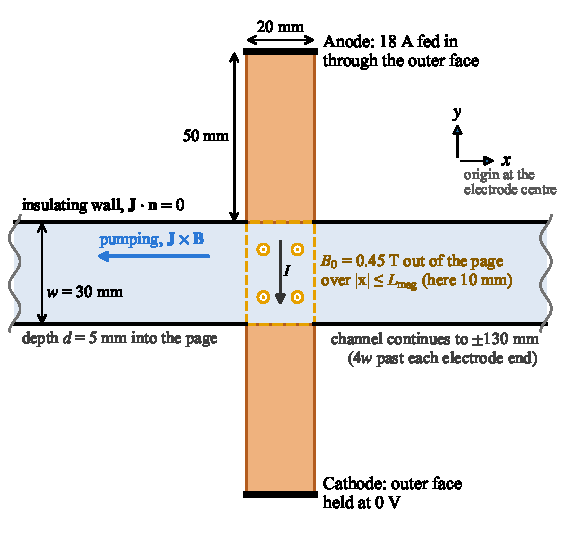
\includegraphics[width=0.6\linewidth]{femm_geometry}
  \caption{Geometry and boundary conditions of the FEMM pump model.}
  \label{fig:femm-geometry}
\end{figure}

\section{Results to Date}

At \SI{18}{\ampere}, the electrode-to-electrode resistance is
\SI{69.6}{\micro\ohm}, and about \SI{40}{\percent} of the current fringes past
the electrode ends, outside the field, where it produces no force
(\cref{fig:femm-jmap}). The model was reduced to a lumped circuit, in which the
Galinstan forms a parasitic path between the electrodes and a fringe path beyond
them, and this circuit reproduced the FEMM force and back-EMF to within
\SI{0.4}{\percent}. From it, the efficiency of the pump has a single peak
(\cref{fig:femm-efficiency}), whose height depends only on the electrode aspect
ratio and the series resistance. \Cref{tab:femm-results} summarises the main
design results.

\begin{figure}[htbp]
  \centering
  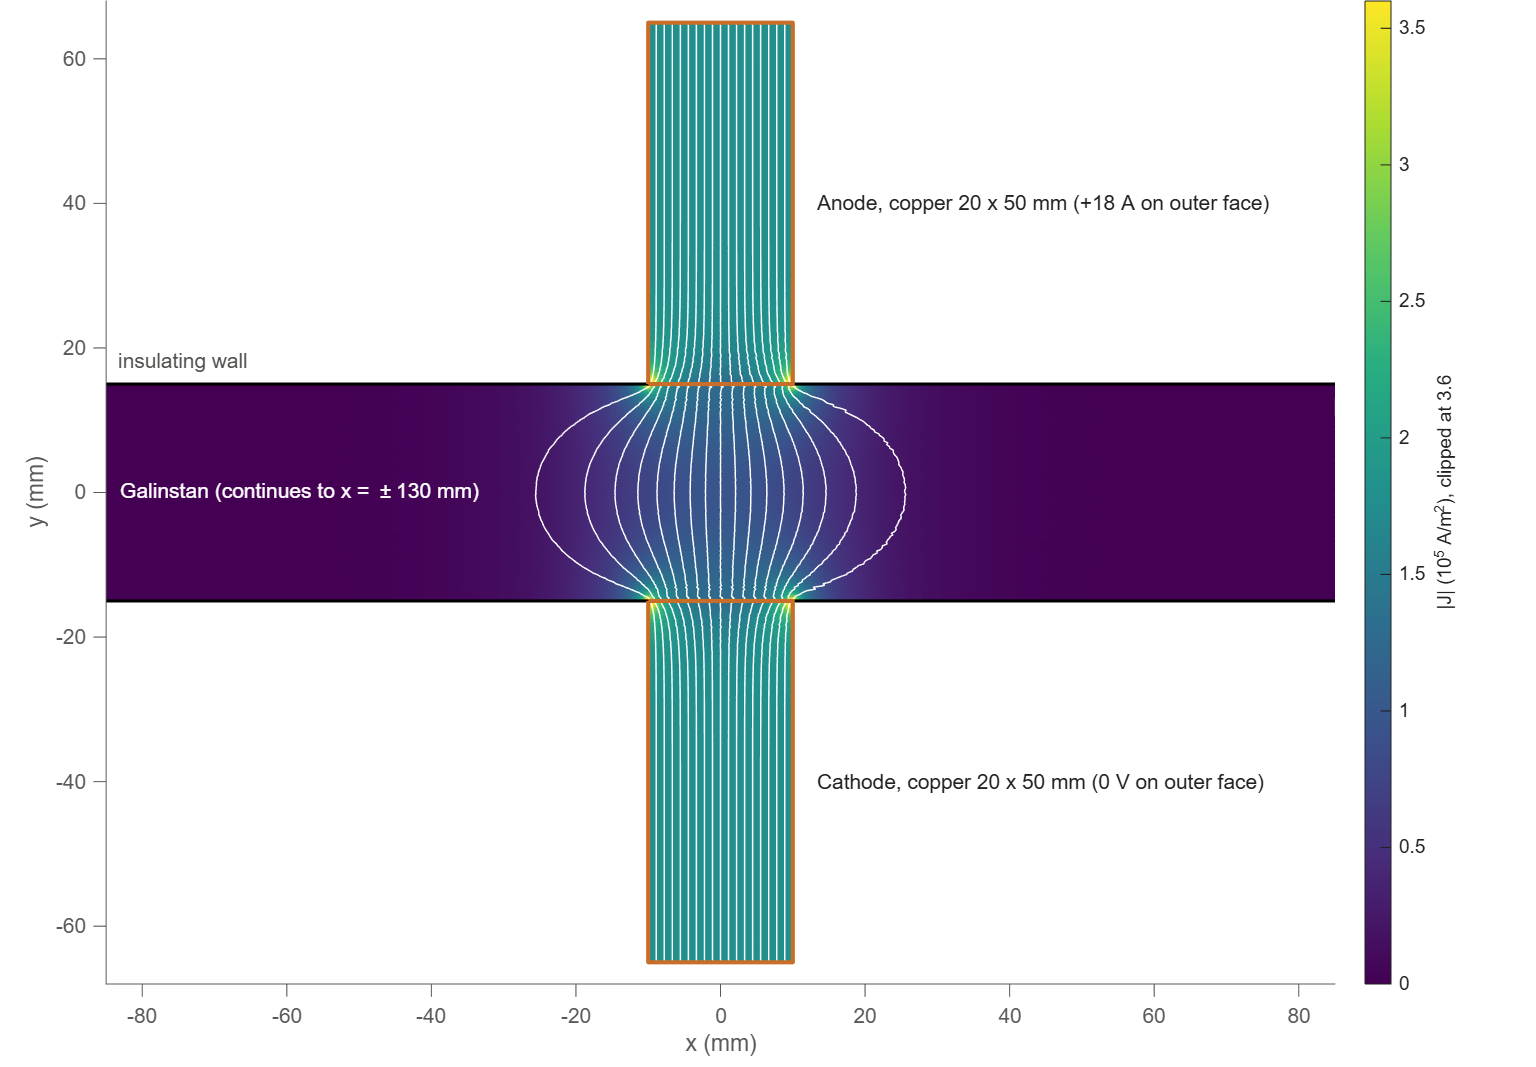
\includegraphics[width=0.6\linewidth]{femm_J_map}
  \caption{Current density in the pump channel at \SI{18}{\ampere}, no flow.}
  \label{fig:femm-jmap}
  \floatnote{Streamlines \SI{1}{\ampere} apart.}
\end{figure}

\begin{figure}[htbp]
  \centering
  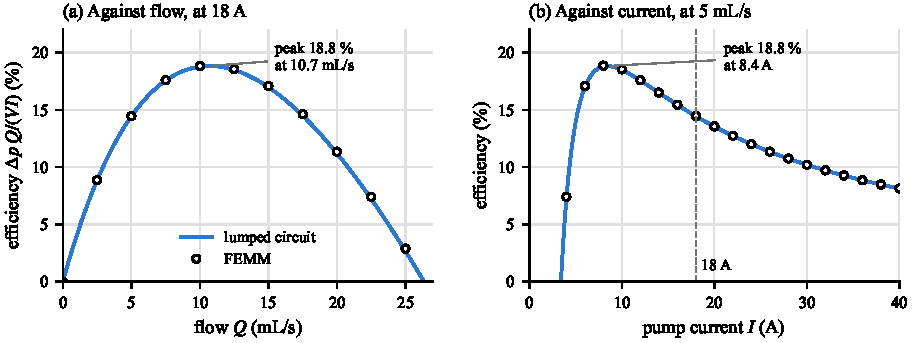
\includegraphics[width=\linewidth]{femm_efficiency}
  \caption{Modelled pump efficiency against flow and current.}
  \label{fig:femm-efficiency}
  \floatnote{\SI{20}{\milli\metre} electrodes, \SI{0.45}{\tesla}; terminal
    efficiency, excluding leads and contacts.}
\end{figure}

\begin{table}[htbp]
  \centering
  \caption{Main results of the FEMM pump model.}
  \label{tab:femm-results}
  \small
  \begin{tabular}{@{}lc@{}}
    \toprule
    Quantity & Value \\
    \midrule
    Electrode-to-electrode resistance & \SI{69.6}{\micro\ohm} \\
    Current inside the field & \SI{60}{\percent} \\
    Zero-flow pressure rise at \SI{18}{\ampere} & \SI{0.98}{\kilo\pascal} \\
    Efficiency at \SI{5}{\milli\litre\per\second}, \SI{18}{\ampere} & \SI{14.5}{\percent} \\
    Peak efficiency, \SI{20}{\milli\metre} electrodes & \SI{18.8}{\percent} \\
    Peak efficiency, \SI{60}{\milli\metre} electrodes & \SI{36.9}{\percent} \\
    Peak efficiency, \SI{20}{\milli\metre} electrodes,
      \SI{50}{\micro\ohm} series resistance & \SI{12.7}{\percent} \\
    \bottomrule
  \end{tabular}
  \floatnote{Terminal efficiency $\Delta p\,Q/(VI)$; the field covers the
    electrodes.}
\end{table}

The design studies suggest three ways to improve the pump. Lengthening the
electrodes, with the field lengthened to match, brings more of the current into
the field and roughly doubles the peak efficiency at \SI{60}{\milli\metre}.
Widening the channel adds flow area but not pressure unless the field is
lengthened with it. A shallower channel gives more pressure per ampere, but at
the cost of higher viscous loss.

The model also points to a likely cause of the low measured efficiency. The
measured pump power of \SI{0.85}{\watt} at \SI{18}{\ampere} corresponds to a
terminal resistance of about \SI{2.6}{\milli\ohm}, nearly 40 times the
\SI{69.6}{\micro\ohm} of the modelled channel and electrodes. Most of the input
power is therefore likely dissipated in the leads, joints and
electrode--Galinstan contacts, which the model does not include. Because the
pump itself is only tens of microohms, even \SI{50}{\micro\ohm} of series
resistance reduces its peak efficiency by about a third
(\cref{tab:femm-results}), so the supply should sit next to the pump on short,
heavy busbars.

\section{Work Remaining}

The model is two-dimensional, so the top and bottom walls, Hartmann layers and
the real velocity profile are not captured, and it assumes a uniform field with
sharp edges, nominal room-temperature conductivities and ideal contacts. To be
used for design, it would need to be validated against measurements of the
pump's pressure--flow curve and terminal voltage, extended to include the
contact and lead resistances and the fringing of the magnet field, and coupled
to the pressure drop of the cooling loop to find the operating point.


\end{document}
"
% =====================================================================
\documentclass[11pt,a4paper,twoside,openany]{report}

% The report class has no \frontmatter, \mainmatter or \backmatter (the book
% class does). Define them as in book.cls for the roman/arabic page numbering:
% with openany they start a new page, with openright a new odd page.
\makeatletter
\providecommand{\frontmatter}{%
  \if@openright\cleardoublepage\else\clearpage\fi\pagenumbering{roman}}
\providecommand{\mainmatter}{%
  \if@openright\cleardoublepage\else\clearpage\fi\pagenumbering{arabic}}
\providecommand{\backmatter}{%
  \if@openright\cleardoublepage\else\clearpage\fi}
\makeatother

\newif\ifreview
\reviewfalse
\ifdefined\REVIEW \reviewtrue \fi

% ---------------------------------------------------------------------
%  Fonts, language and page geometry
% ---------------------------------------------------------------------
\usepackage[T1]{fontenc}
\usepackage[utf8]{inputenc}
\usepackage{lmodern}                 % Computer Modern in T1 (as in Lawton)
\usepackage[british]{babel}          % NZ/UK spelling and hyphenation
\usepackage{microtype}
% Compact layout: narrow margins and near-single spacing, so that the body
% (Introduction to Conclusion) fits within 30 pages.
\usepackage[a4paper,top=20mm,bottom=20mm,inner=20mm,outer=20mm,
            headheight=14pt,headsep=6mm,footskip=10mm]{geometry}
\usepackage{setspace}
\setstretch{1.05}
\setlength{\emergencystretch}{1.5em}

% Display faces used for the title page and chapter openers
\newcommand{\chapnumfont}{\fontfamily{ppl}\fontseries{b}\selectfont}  % Palatino bold
\newcommand{\titlefont}{\fontfamily{bch}\fontseries{b}\selectfont}    % Charter bold

% ---------------------------------------------------------------------
%  Maths, units, tables, figures
% ---------------------------------------------------------------------
\usepackage{amsmath,amssymb}
\usepackage{siunitx}
\sisetup{
  per-mode            = symbol,
  inter-unit-product  = \ensuremath{\cdot},
  range-phrase        = --,
  range-units         = single,
  list-final-separator= {, and },
  product-units       = single,
}
\usepackage{graphicx}
\graphicspath{{figures/}}
\usepackage{booktabs,tabularx,array,multirow,makecell,longtable}
\renewcommand{\arraystretch}{1.15}
\newcolumntype{L}{>{\raggedright\arraybackslash}X}
\newcolumntype{C}{>{\centering\arraybackslash}X}
\usepackage{xcolor}
\definecolor{uoablue}{RGB}{0,70,127}
\usepackage{enumitem}
\setlist{itemsep=0pt,topsep=4pt}
\usepackage[labelsep=colon,skip=6pt]{caption}
\captionsetup[table]{position=top}
% All captions flush left, so short and long captions (and the notes below
% them) line up the same way.
\captionsetup{singlelinecheck=false}
% Captions are a short title only. Any further detail goes in a concise note:
% under the caption of a figure, or under the body of a table. \tnote marks
% the table cell that a note refers to.
\newcommand{\floatnote}[1]{\par\vspace{3pt}%
  {\raggedright\footnotesize\textit{Note:} #1\par}}
\newcommand{\tnote}[1]{\textsuperscript{#1}}
\usepackage{float}
\usepackage{placeins}                % \FloatBarrier keeps floats in their section
% Float placement. With LaTeX's defaults most floats here ended up on sparse
% float-only pages, centred vertically, away from the text that cites them.
% Allow more and larger floats on text pages (floats use [htbp]), accept a
% float-only page only when it is at least 3/4 full, and stack the floats at
% the top of such a page instead of spreading them down it.
\setcounter{topnumber}{3}
\setcounter{bottomnumber}{2}
\setcounter{totalnumber}{4}
\renewcommand{\topfraction}{0.85}
\renewcommand{\bottomfraction}{0.6}
\renewcommand{\textfraction}{0.12}
\renewcommand{\floatpagefraction}{0.75}
% When a page with floats cannot be filled exactly (e.g. the next heading does
% not fit), open up the gap between the floats and the text rather than the
% spacing between paragraphs.
\setlength{\textfloatsep}{14pt plus 12pt minus 4pt}
\setlength{\floatsep}{10pt plus 4pt minus 2pt}
\setlength{\intextsep}{10pt plus 4pt minus 2pt}
\makeatletter
\setlength{\@fptop}{0pt}
\setlength{\@fpsep}{\floatsep}
\setlength{\@fpbot}{0pt plus 1fil}
\makeatother
\usepackage{pdfpages}                % signed statement of contribution
\usepackage{nomencl}                 % nomenclature (ECSE template)
\makenomenclature
\usepackage[titles]{tocloft}         % TOC/LOF/LOT entries as in the ECSE template

\usepackage{subcaption}
% Subfigures: centred "(a) ..." captions, cited as "Fig. 4.5(a)"
\captionsetup[sub]{singlelinecheck=true,labelformat=simple}
\renewcommand{\thesubfigure}{(\alph{subfigure})}
\usepackage{pgfplots}
 \pgfplotsset{compat=1.17}
\usepgfplotslibrary{groupplots}      % multi-panel transient figures
\usepackage[american]{circuitikz}    % thermal network figure

% ---------------------------------------------------------------------
%  Headings
% ---------------------------------------------------------------------
\usepackage{titlesec}
% Chapter heading: bold Computer Modern, flush left, number and title on one
% line at the top of the page (compact layout).
\newcommand{\bodychapterformat}{%
  \titleformat{\chapter}[hang]
    {\normalfont\LARGE\bfseries\raggedright}
    {\thechapter}
    {0.8em}
    {}%
  \titleformat{name=\chapter,numberless}[hang]
    {\normalfont\LARGE\bfseries\raggedright}
    {}
    {0pt}
    {}%
  \titlespacing*{\chapter}{0pt}{0pt}{16pt}}
\bodychapterformat
\titleformat{\section}{\normalfont\large\bfseries}{\thesection}{1em}{}
\titleformat{\subsection}{\normalfont\normalsize\bfseries}{\thesubsection}{1em}{}
\titleformat{\subsubsection}{\normalfont\normalsize\bfseries}{\thesubsubsection}{1em}{}
\titlespacing*{\section}{0pt}{2.2ex plus .8ex minus .2ex}{1.0ex plus .2ex}
\titlespacing*{\subsection}{0pt}{1.8ex plus .6ex minus .2ex}{0.8ex plus .2ex}
\titlespacing*{\subsubsection}{0pt}{1.6ex plus .6ex minus .2ex}{0.5ex plus .2ex}
\setcounter{secnumdepth}{2}
\setcounter{tocdepth}{2}

% Front-matter headings follow the ECSE template (14 pt bold, flush left);
% \bodyheadings restores the body chapter heading for the main matter.
\newcommand{\frontheadings}{%
  \titleformat{name=\chapter,numberless}[block]
    {\normalfont\fontsize{14}{17}\selectfont\bfseries}{}{0pt}{}%
  \titlespacing*{\chapter}{0pt}{0pt}{12pt}}
\newcommand{\bodyheadings}{\bodychapterformat}

% ---------------------------------------------------------------------
%  ECSE template settings for the front matter
% ---------------------------------------------------------------------
\newcommand\HRule{\noindent\rule{\linewidth}{2pt}}   % title-page rules
\addto\captionsbritish{\renewcommand{\contentsname}{Table of Contents}}
% "Figure"/"Table" prefixes in the lists of figures and tables
\renewcommand{\cftfigpresnum}{Figure~}
\renewcommand{\cfttabpresnum}{Table~}
\setlength{\cftfignumwidth}{5.2em}
\setlength{\cfttabnumwidth}{5.2em}
% Nomenclature: "Symbols" / "Greek Symbols" groups with a unit column
\renewcommand{\nomname}{Nomenclature}
\def\nompreamble{\addcontentsline{toc}{chapter}{\nomname}\markboth{\nomname}{\nomname}}
\renewcommand{\nomgroup}[1]{%
  \ifthenelse{\equal{#1}{A}}{\item[\textbf{Symbols}]}{%
  \ifthenelse{\equal{#1}{G}}{\item[\textbf{Greek Symbols}]}{}}}
\newcommand{\nomunit}[1]{\renewcommand{\nomentryend}{\hspace*{\fill}#1}}
\setlength{\nomlabelwidth}{2.6cm}
\usepackage{ifthen}

% ---------------------------------------------------------------------
%  Running heads (Lawton: bold, ruled; page number outside;
%  chapter title on even pages, section on odd pages)
% ---------------------------------------------------------------------
\usepackage{fancyhdr}
\renewcommand{\chaptermark}[1]{\markboth{#1}{#1}}
\renewcommand{\sectionmark}[1]{\markright{\thesection\ \ #1}}
\fancypagestyle{lawton}{%
  \fancyhf{}%
  \fancyhead[LE]{\bfseries\thepage}%
  \fancyhead[RE]{\bfseries\nouppercase{\leftmark}}%
  \fancyhead[LO]{\bfseries\nouppercase{\rightmark}}%
  \fancyhead[RO]{\bfseries\thepage}%
  \renewcommand{\headrulewidth}{0.4pt}}
\pagestyle{lawton}
% Chapter opening pages use the plain style; in the body, give them the same
% ruled running head as every other page.
\newcommand{\bodyplainstyle}{%
  \fancypagestyle{plain}{%
    \fancyhf{}%
    \fancyhead[LE]{\bfseries\thepage}%
    \fancyhead[RE]{\bfseries\nouppercase{\leftmark}}%
    \fancyhead[LO]{\bfseries\nouppercase{\rightmark}}%
    \fancyhead[RO]{\bfseries\thepage}%
    \renewcommand{\headrulewidth}{0.4pt}}}
% ECSE template: no header, small centred page number
\fancypagestyle{front}{%
  \fancyhf{}%
  \fancyfoot[C]{\footnotesize\thepage}%
  \renewcommand{\headrulewidth}{0pt}}
\newcommand{\frontplainstyle}{%
  \fancypagestyle{plain}{%
    \fancyhf{}%
    \fancyfoot[C]{\footnotesize\thepage}%
    \renewcommand{\headrulewidth}{0pt}}}

% ---------------------------------------------------------------------
%  References (IEEE, with DOIs as in Lawton; source: Zotero export)
% ---------------------------------------------------------------------
\usepackage{csquotes}
\usepackage[backend=biber,style=ieee,
            doi=true,url=true,isbn=false,dashed=false,maxnames=6,minnames=1]{biblatex}
\addbibresource{zotero_references.bib}
\AtEveryBibitem{\clearfield{issn}%
  % an access date means nothing without a URL (e.g. Zotero items with no link)
  \iffieldundef{url}{\clearfield{urlyear}\clearfield{urlmonth}\clearfield{urlday}}{}}
% zotero_references.bib is the Zotero export; tidy its fields here rather than
% editing the file, so the fixes survive a refresh from Zotero. Drop language
% tags, ISBNs and the "ISSN: ..." notes Zotero writes, and give items that have
% a DOI only the DOI (no URL or access date).
\DeclareSourcemap{
  \maps[datatype=bibtex]{
    \map{
      \step[fieldset=language, null]
      \step[fieldset=isbn, null]
      \step[fieldsource=note, match=\regexp{\AISSN:}, final]
      \step[fieldset=note, null]
    }
    \map{
      \step[fieldsource=doi, final]
      \step[fieldset=url, null]
      \step[fieldset=urldate, null]
    }
    % Zotero stores an article number (e.g. 100133) as the page range; print it
    % as "Art. no." rather than as a page number
    \map{
      \pertype{article}
      \step[fieldsource=pages, notmatch=\regexp{-}, final]
      \step[fieldset=eid, origfieldval]
      \step[fieldset=pages, null]
    }
  }
}
\DeclareFieldFormat[article]{eid}{Art\adddot\space no\adddot\space#1}
% Some Zotero titles carry a zero-width space (U+200B), which pdfLaTeX cannot
% typeset; drop it here so the fix survives a refresh from Zotero. Also allow a
% line break after a Unicode em dash (U+2014), so that long titles such as
% Ouyang's do not run into the margin.
\DeclareUnicodeCharacter{200B}{}
\DeclareUnicodeCharacter{2014}{\textemdash\allowbreak}
% Break long DOIs and URLs without stretching the gaps around "." and "/"
\setcounter{biburlnumpenalty}{9000}
\setcounter{biburlucpenalty}{9000}
\setcounter{biburllcpenalty}{9000}
\biburlbigskip=0mu plus 1mu\relax

% ---------------------------------------------------------------------
%  Cross-referencing
% ---------------------------------------------------------------------
\usepackage[hidelinks,bookmarksnumbered]{hyperref}
\usepackage[nameinlink]{cleveref}
\crefname{chapter}{Chapter}{Chapters}
\crefname{section}{Section}{Sections}
\crefname{subsection}{Section}{Sections}
\crefname{figure}{Fig.}{Figs.}
\Crefname{figure}{Figure}{Figures}
\crefname{table}{Table}{Tables}
\crefname{appendix}{Appendix}{Appendices}
\crefname{subappendix}{Appendix}{Appendices}
\crefname{equation}{}{}
\crefformat{equation}{(#2#1#3)}
\crefrangeformat{equation}{(#3#1#4)--(#5#2#6)}
\crefmultiformat{equation}{(#2#1#3)}{ and~(#2#1#3)}{, (#2#1#3)}{ and~(#2#1#3)}

% ---------------------------------------------------------------------
%  Review notes
% ---------------------------------------------------------------------
\ifreview
  \usepackage[colorinlistoftodos,textsize=small]{todonotes}
    \newcommand{\issue}[1]{\par\todo[inline,color=orange!20,bordercolor=orange!70!black,
      linecolor=orange!70!black,caption={\textsc{Issue}: #1}]{\textbf{Issue:} #1}}
  \newcommand{\edited}[1]{\par\todo[inline,color=cyan!12,bordercolor=cyan!50!black,
      linecolor=cyan!50!black,caption={\textsc{Edited}: #1}]{\textbf{Edited:} #1}}
\else
  \newcommand{\issue}[1]{\ignorespaces}
  \newcommand{\edited}[1]{\ignorespaces}
\fi
% A value or detail still to be supplied. Always shown, in red, so that it
% cannot be missed in a submitted copy.
\newcommand{\missing}[1]{\textcolor{red}{[#1]}}
% \figureorplaceholder[options]{file}: as \includegraphics, but while
% figures/<file> does not exist yet it draws a framed placeholder naming the
% file, so the report still compiles.
\newcommand{\figureorplaceholder}[2][]{%
  \IfFileExists{figures/#2}{\includegraphics[#1]{#2}}{%
    \fbox{\parbox[c][4cm][c]{0.85\linewidth}{\centering
      \missing{Figure to be added: figures/\detokenize{#2}}}}}}

% ---------------------------------------------------------------------
%  Convenience macros
% ---------------------------------------------------------------------
\newcommand{\Vdot}{\dot{V}}
\newcommand{\mdot}{\dot{m}}
\newcommand{\cp}{c_{\mathrm{p}}}
\newcommand{\NTU}{\mathrm{NTU}}
\newcommand{\Rcp}{R_{\mathrm{cp}}}
\newcommand{\Rpack}{R_{\mathrm{pack}}}
\newcommand{\Rmisc}{R_{\mathrm{misc}}}
\newcommand{\Qin}{Q_{\mathrm{in}}}
\newcommand{\Qplate}{Q_{\mathrm{plate}}}
\newcommand{\Tin}{T_{\mathrm{in}}}
\newcommand{\Tout}{T_{\mathrm{out}}}
\newcommand{\Tres}{T_{\mathrm{resistor}}}
\newcommand{\Galinstan}{Galinstan}
\newcommand{\GaInSn}[3]{Ga\textsubscript{#1}In\textsubscript{#2}Sn\textsubscript{#3}}

% ---------------------------------------------------------------------
%  Report details (edit here)
% ---------------------------------------------------------------------
\newcommand{\reporttitle}{Liquid Metal Cooling for High-Power-Density Power Electronic Converters}
\newcommand{\reportauthor}{Alex Skilton}
\newcommand{\reporttype}{Final Report}
\newcommand{\reportdate}{\number\day\ \ifcase\month\or January\or February\or March\or April\or May\or June\or July\or August\or September\or October\or November\or December\fi\ \number\year}
\newcommand{\reportpartner}{Shrirang Ekbote}
\newcommand{\reportsupervisor}{Dr. Patrick Lawton and Prof. Grant Covic}

\hypersetup{pdftitle={\reporttitle},pdfauthor={\reportauthor}}

% =====================================================================
\begin{document}

\frontmatter
\frontheadings
\frontplainstyle
\pagestyle{empty}
%% =====================================================================
%  Title page -- 2026 ECSE Part IV Final Report template
%  (layout, rules, sizes and logo as in mainDocument.tex of the template;
%  type sizes are fixed at the template's 12 pt values)
% =====================================================================
\begin{titlepage}
\newgeometry{top=2cm,bottom=2cm,left=2.5cm,right=2.5cm}
\begin{spacing}{1}
\fontsize{12}{14.5}\selectfont
\setlength{\parindent}{0pt}
\setlength{\parskip}{\medskipamount}

\vspace*{10mm}

\begin{center}
\textbf{\fontsize{14.4}{18}\selectfont Research Project Report}
\end{center}

\vspace*{10mm}

\HRule
\begin{center}
\reporttype
\end{center}

\begin{center}
\textbf{\fontsize{17.28}{22}\selectfont \reporttitle}
\end{center}

\begin{center}
{\fontsize{14.4}{18}\selectfont \reportauthor}
\end{center}

\HRule

\vspace*{\fill}

\begin{center}
\begin{tabular}{rl}
Partner:  & \reportpartner \\
\noalign{\vskip1.5em}
Supervisor: & \reportsupervisor \\
\noalign{\vskip1.5em}
\end{tabular}
\end{center}

\vspace*{\fill}

\begin{center}
\reportdate
\end{center}

\vspace*{\fill}

\begin{center}

\includegraphics[width=0.7\linewidth]{UoA-Logo-Primary-RGB-Large}
\end{center}

\end{spacing}
\restoregeometry
\end{titlepage}


\pagestyle{front}
%% =====================================================================
%  Abstract page -- ECSE template layout
% =====================================================================
\thispagestyle{front}
\begingroup
\setlength{\parindent}{0pt}
\setlength{\parskip}{9pt}

\vspace*{1em}

\begin{center}
\textbf{\large \MakeUppercase{\reporttitle}}
\end{center}

\vspace{2em}

\begin{center}
\textbf{\large \reportauthor}
\end{center}

\vspace{2em}

\begin{center}
\textbf{\large ABSTRACT}
\end{center}

% Write your abstract here
[Abstract to be written.]
% end of Abstract

\endgroup
\clearpage


% Signed Statement of Contribution (student + supervisor). Replace
% frontmatter/Declaration.pdf with the signed copy.
% 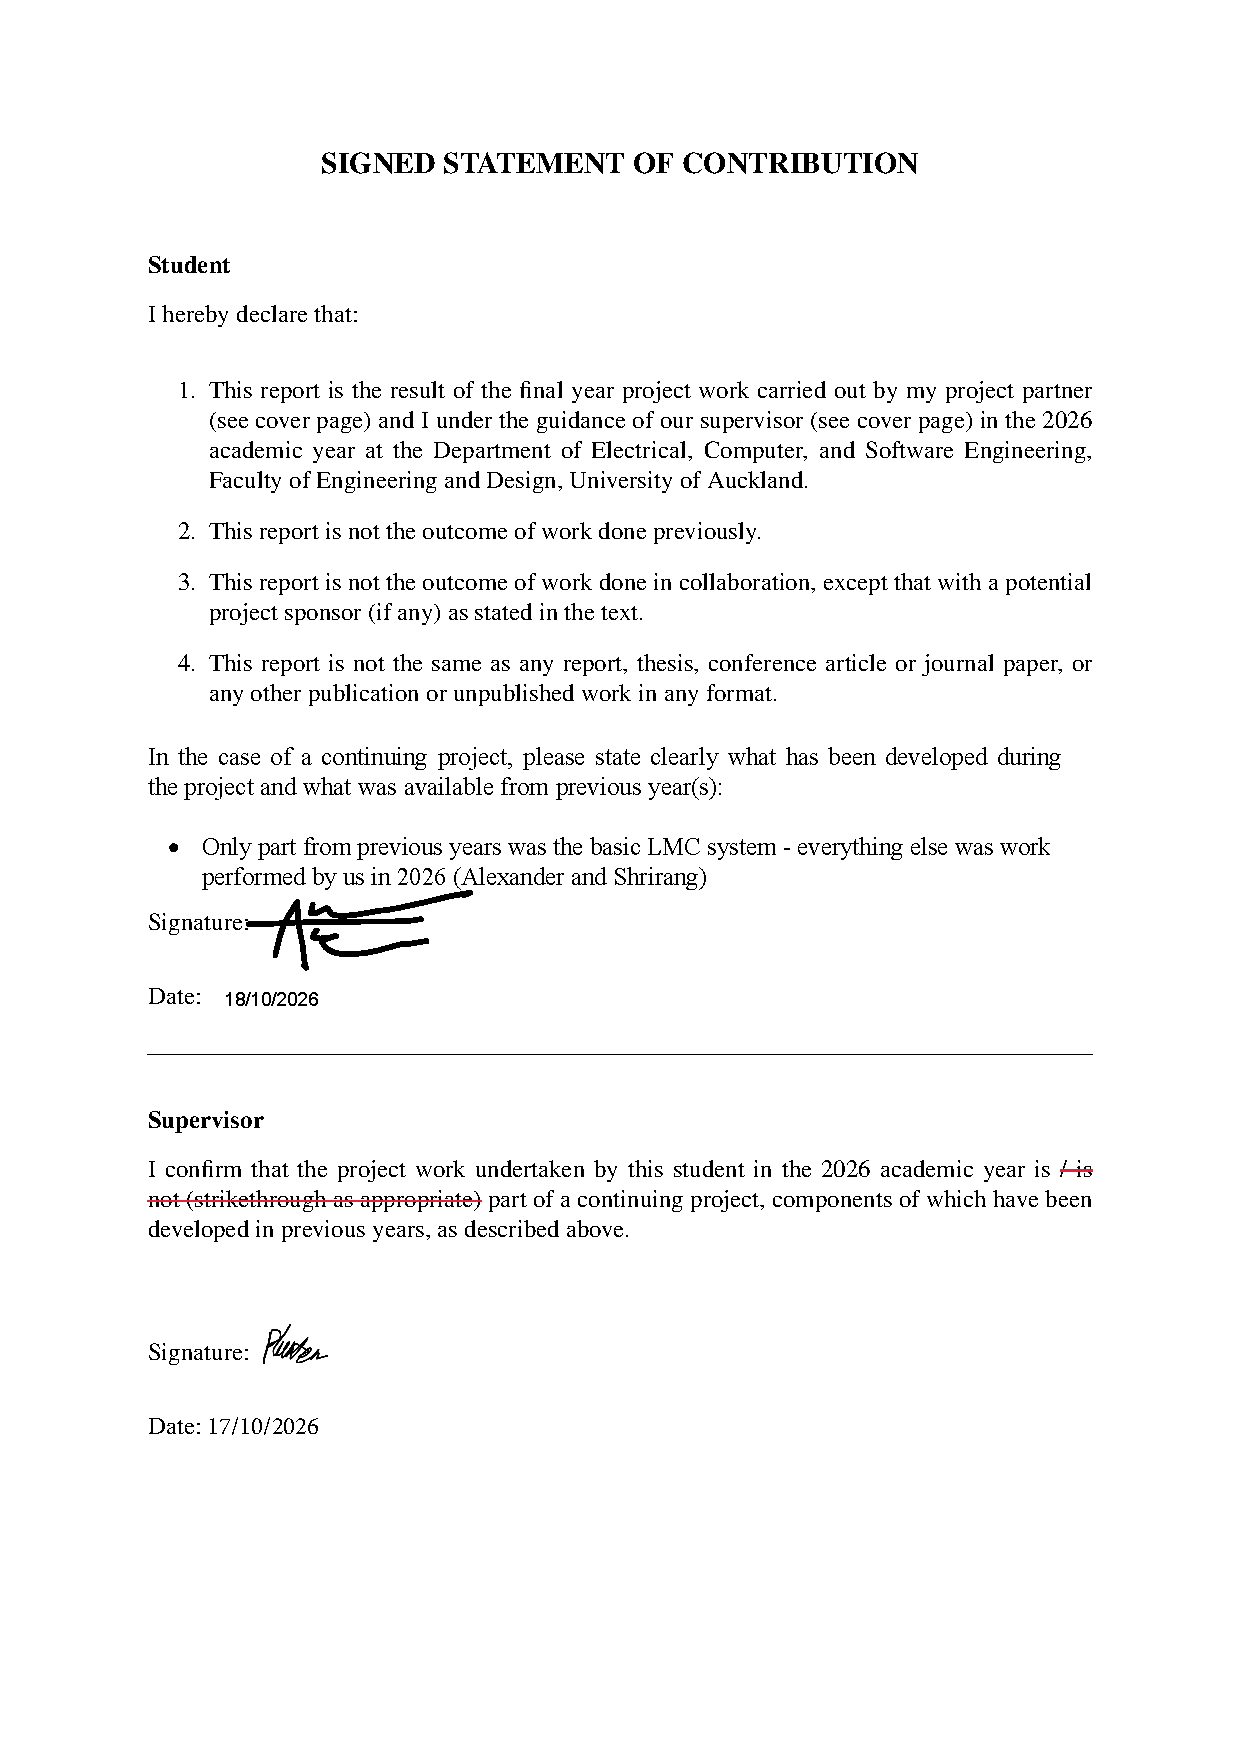
\includepdf[pagecommand=\thispagestyle{front}]{frontmatter/Declaration PAT SIGNED}
% \tableofcontents
% \listoffigures
% \listoftables
% % =====================================================================
%  Acknowledgements -- ECSE template
% =====================================================================
\chapter*{Acknowledgements}
\addcontentsline{toc}{chapter}{Acknowledgements}
\begingroup
\setlength{\parindent}{0pt}
\setlength{\parskip}{9pt}

Firstly, I would like to acknowledge my parents for their consistent love and support throughout my studies.

I would also like to express my sincere appreciation to my friend and project partner, Shrirang Ekbote, for his contributions, teamwork, and companionship throughout this project. It has been a long yet rewarding final year at university, and I look forward to continuing our journey together out in the professional world.

Thank you to my supervisors, Dr. Patrick Lawton and Professor Grant Covic, for their dedicated support, guidance, and expertise throughout this project. I truly appreciated your honest feedback and the time you took out of your busy schedules to encourage us when motivation was low. The lessons from this experience have undoubtedly made me a better engineer, and I will carry them with me into the future.

I would like to thank Cody Liu, Thor Bridger, Taha Basar, Howard Lu and the rest of the ECSE Power Electronics Lab for always being willing to help and contributing to a safe and functioning lab environment. 

Finally, thank you to all my other friends in the rest of the department and beyond, for contributing to the conversations, jokes, and memories throughout this year.

\endgroup

% % =====================================================================
%  Glossary of Terms -- ECSE template (Term / Definition longtable)
%  Definitions follow the usage in the report body; edit as needed.
% =====================================================================
\chapter*{Glossary of Terms}
\addcontentsline{toc}{chapter}{Glossary of Terms}

\begin{longtable}[l]{>{\raggedright}p{0.25\textwidth}>{\raggedright\arraybackslash}p{0.68\textwidth}}
\textbf{Term} & \textbf{Definition} \\
\addlinespace
Caloric resistance & Coolant temperature rise per unit heat load, $1/(\rho\,\cp\,\Vdot)$; the part of the thermal resistance set by the coolant's heat-capacity rate. \\
\addlinespace
Cold plate & Metal plate with internal coolant passages onto which heat-dissipating components are mounted. \\
\addlinespace
Conduction pump & Electromagnetic pump that drives a conductive liquid by passing a DC current through it across a magnetic field, producing a Lorentz force. \\
\addlinespace
Eddy current & Current induced in a conductor by a time-varying magnetic field, dissipating power as heat. \\
\addlinespace
Effectiveness & Ratio of the heat actually absorbed by the coolant to the maximum possible for the given inlet and wall temperatures. \\
\addlinespace
Galinstan & Eutectic gallium--indium--tin alloy that is liquid at room temperature. \\
\addlinespace
Power density & Power processed by a converter per unit volume. \\
\addlinespace
Skin depth & Depth at which an alternating current or field in a conductor has decayed to $1/e$ of its surface value. \\
\addlinespace
Thermal resistance & Temperature difference per unit heat flow between two points, in \si{\kelvin\per\watt}. \\
\end{longtable}
\addtocounter{table}{-1}

% % Abbreviations -- ECSE template layout (two-column longtable)
\chapter*{Abbreviations}
\addcontentsline{toc}{chapter}{Abbreviations}

\begin{longtable}[l]{>{\raggedright}p{0.25\textwidth}>{\raggedright\arraybackslash}p{0.68\textwidth}}
  AC    & Alternating current \\
  AI    & Artificial intelligence \\
  CAD   & Computer-aided design \\
  CHF   & Critical heat flux \\
  DC    & Direct current \\
  DCM   & Discontinuous conduction mode \\
  EM    & Electromagnetic \\
  EMF   & Electromotive force \\
  EV    & Electric vehicle \\
  Ga    & Gallium \\
  GaInSn & Gallium--indium--tin alloy (Galinstan) \\
  GaN   & Gallium nitride \\
  IPT   & Inductive power transfer \\
  LCC   & Inductor--capacitor--capacitor (compensation network) \\
  LCR   & Inductance--capacitance--resistance (meter) \\
  MHD   & Magnetohydrodynamic \\
  NaK   & Sodium--potassium alloy \\
  NTU   & Number of transfer units \\
  PEC   & Power electronic converter \\
  PFA   & Perfluoroalkoxy (polymer tubing) \\
  RQ    & Research question \\
  SiC   & Silicon carbide \\
  SMR   & Small modular reactor \\
  TIM   & Thermal interface material \\
  VA    & Volt-ampere \\
  ZVS   & Zero-voltage switching \\
\end{longtable}
\addtocounter{table}{-1}

% % Nomenclature (ECSE template: nomencl package, 'Symbols' and 'Greek Symbols'
% groups, unit in right-hand column). Prefix A = Symbols, G = Greek; the rest
% of the prefix is the sort key.

\nomenclature[Aa]{$A$}{Heat-transfer area of the cold-plate tube\nomunit{\si{\metre\squared}}}
\nomenclature[Ab]{$B$}{Magnetic flux density\nomunit{\si{\tesla}}}
\nomenclature[Actarget]{$C_{\mathrm{target}}$}{Target tuning capacitance\nomunit{\si{\farad}}}
\nomenclature[Acp]{$\cp$}{Specific heat capacity at constant pressure\nomunit{\si{\joule\per\kilogram\per\kelvin}}}
\nomenclature[Adh]{$D_{\mathrm{h}}$}{Hydraulic diameter\nomunit{\si{\metre}}}
\nomenclature[Ae]{$E$}{EMF measured by the flow sensor\nomunit{\si{\volt}}}
\nomenclature[Af]{$f$}{Frequency\nomunit{\si{\hertz}}}
\nomenclature[Ah]{$h$}{Convective heat transfer coefficient\nomunit{\si{\watt\per\metre\squared\per\kelvin}}}
\nomenclature[Ai1]{$I_{1}$}{Primary resonant current (rms)\nomunit{\si{\ampere}}}
\nomenclature[Ak]{$k$}{Thermal conductivity\nomunit{\si{\watt\per\metre\per\kelvin}}}
\nomenclature[Al]{$L$}{Heated tube length\nomunit{\si{\metre}}}
\nomenclature[Al1]{$L_{1}$}{Primary (inductor) self-inductance\nomunit{\si{\henry}}}
\nomenclature[Alg]{$l_{\mathrm{g}}$}{Air-gap length\nomunit{\si{\metre}}}
\nomenclature[Amdot]{$\mdot$}{Mass flow rate\nomunit{\si{\kilogram\per\second}}}
\nomenclature[An]{$N$}{Number of turns\nomunit{}}
\nomenclature[Anf]{$N_{\mathrm{f}}$}{Number of power cycles to failure\nomunit{cycles}}
\nomenclature[Anu]{Nu}{Nusselt number\nomunit{}}
\nomenclature[Antu]{NTU}{Number of transfer units, $hA/(\mdot\,\cp)$\nomunit{}}
\nomenclature[Ap]{$P$}{Tube perimeter\nomunit{\si{\metre}}}
\nomenclature[Aqqin]{$Q$, $\Qin$}{Heat load; input heat\nomunit{\si{\watt}}}
\nomenclature[Aqplate]{$\Qplate$}{Heat transferred into the cold plate\nomunit{\si{\watt}}}
\nomenclature[Arac]{$R_{\mathrm{ac}}$}{AC winding resistance\nomunit{\si{\ohm}}}
\nomenclature[Arcp]{$\Rcp$}{Cold-plate thermal resistance\nomunit{\si{\kelvin\per\watt}}}
\nomenclature[Armisc]{$\Rmisc$}{Thermal resistance to ambient\nomunit{\si{\kelvin\per\watt}}}
\nomenclature[Arpack]{$\Rpack$}{Package (resistor and interface) thermal resistance\nomunit{\si{\kelvin\per\watt}}}
\nomenclature[Are]{Re}{Reynolds number\nomunit{}}
\nomenclature[Ata]{$T_{\mathrm{A}}$}{Ambient temperature\nomunit{\si{\celsius}}}
\nomenclature[Atfx]{$T_{\mathrm{f}}(x)$}{Local coolant temperature\nomunit{\si{\celsius}}}
\nomenclature[Atintout]{$\Tin$, $\Tout$}{Coolant inlet and outlet temperatures\nomunit{\si{\celsius}}}
\nomenclature[Atj]{$T_{\mathrm{j}}$}{Junction temperature\nomunit{\si{\celsius}}}
\nomenclature[Atm]{$T_{\mathrm{M}}$}{Resistor (heat-source) node temperature\nomunit{\si{\celsius}}}
\nomenclature[Atp]{$T_{\mathrm{P}}$}{Isothermal plate node temperature\nomunit{\si{\celsius}}}
\nomenclature[Avdc]{$V_{\mathrm{DC}}$}{DC bus voltage\nomunit{\si{\volt}}}
\nomenclature[Avdot]{$\Vdot$}{Volumetric flow rate\nomunit{\si{\metre\cubed\per\second}}}
\nomenclature[Axres]{$X_{\mathrm{res}}$}{Resonant reactance\nomunit{\si{\ohm}}}
\nomenclature[Galphabeta]{$\alpha$, $\beta$}{Coffin--Manson fitting parameters\nomunit{}}
\nomenclature[Gdelta]{$\delta$}{Skin depth\nomunit{\si{\metre}}}
\nomenclature[Gdeltat]{$\Delta T$}{Temperature rise or swing\nomunit{\si{\kelvin}}}
\nomenclature[Gvarepsilon]{$\varepsilon$}{Cold-plate effectiveness\nomunit{}}
\nomenclature[Gmu]{$\mu$}{Dynamic viscosity\nomunit{\si{\pascal\second}}}
\nomenclature[Gmu0]{$\mu_{0}$}{Permeability of free space\nomunit{\si{\henry\per\metre}}}
\nomenclature[Grho]{$\rho$}{Density\nomunit{\si{\kilogram\per\metre\cubed}}}
\nomenclature[Gsigma]{$\sigma$}{Electrical conductivity\nomunit{\si{\siemens\per\metre}}}

% \printnomenclature
% \ifreview
%   \listoftodos[Review Notes]
% \fi

\clearpage{\pagestyle{empty}\cleardoublepage}% blank verso (if any) without a page number
\mainmatter
\bodyheadings
\bodyplainstyle
\pagestyle{lawton}
% =====================================================================
%  Chapter 1 -- Introduction (limited to one page)
% =====================================================================
\chapter{Introduction}
\label{ch:Introduction}

The continued electrification of the global economy is driving a sustained
increase in electricity demand~\cite{international_energy_agency_electricity_2025}.
Power electronic converters (PECs) enable this shift by electrifying
transport~\cite{bosshard_multi-objective_2016} and energy
systems~\cite{steimer_enabled_2010}. The power density of PECs has risen for decades,
driven by cost, functionality and hard weight and space
limits~\cite{steimer_enabled_2010,biela_cooling_2007}, and is projected to keep
rising~\cite{morroni_understanding_2023}. As converters shrink, however, the
same losses must be removed from a smaller volume, so thermal management
increasingly limits how far power density can
rise~\cite{biela_cooling_2007,morroni_understanding_2023}.

Inductive power transfer (IPT) chargers for electric vehicles illustrate this
challenge. At the standard \SI{85}{\kilo\hertz}~\cite{society_of_automotive_engineers_r_2024},
a \SI{10}{\kilo\watt} system dissipates several hundred watts, much of it in pads
that generate strong alternating magnetic fields~\cite{kim_thermal_2022}. Many
commercial designs already actively cool the coils~\cite{lawton_power_2024}, and
Liu \emph{et al.}\ call for new technologies to cool wireless
chargers~\cite{liu_thermal_2025}. Water cooling, however, is limited by the low
thermal conductivity of water~\cite{laloya_heat_2016}. Galinstan, a liquid metal
with much higher thermal conductivity~\cite{noauthor_gainsn_nodate}, can instead
be driven by a magnetohydrodynamic (MHD) pump with no moving
parts~\cite{hodes_potential_2014}, but its low volumetric heat capacity and
electrical conductivity bring trade-offs~\cite{hodes_potential_2014,an_liquid_2024}.
The extent of its advantage therefore remains unclear, as few studies compare it
with water at converter scale~\cite{fan_ultra-efficient_2026}.

This project builds on the 2025 Part~IV Project~\#51, in which Kwon and Loh
built an MHD-pumped Galinstan cooling loop and recommended comparing it with
water cooling and testing it near magnetic
components~\cite{kwon_project_2025,loh_project_2025}. Its aim is to evaluate
MHD-pumped Galinstan as a coolant for high-power-density PECs, and to identify
where in an IPT system it is most useful. The objectives are to (i)~compare the
thermal resistance and pumping power of the Galinstan loop with those of a water
loop using the same cold plate~\cite{ekbote_project_2026}; (ii)~explain and
extend the measurements with thermal models and a conjugate heat transfer
simulation; and (iii)~use a power-dense \SI{85}{\kilo\hertz} inductor to
demonstrate Galinstan cooling of magnetics and measure the eddy-current loss
induced in the coolant. These objectives are framed as two research questions
in \cref{sec:research-questions}. \Cref{ch:literature} reviews the literature,
\cref{ch:experimental} describes the methodology, \cref{ch:results} presents
the results, \cref{sec:discussion} discusses them and \cref{ch:conclusion}
concludes the report.

% =====================================================================
%  Chapter 2 -- Literature Review   (source: Literature_Review_Draft_v9.docx)
% =====================================================================
\chapter{Literature Review}
\label{ch:literature}
\edited{Section 2.3 restructured under three requirements (reliability, form
factor, efficiency), each comparing single-phase and phase-change cooling and
their implications for magnetic components. \Cref{tab:cooling-strategies} is
regrouped to match, with an added row for loss in magnetics.}

This chapter reviews the literature on cooling power electronic converters
(PECs) with liquid metal. It opens with the sources of loss in inductive power
transfer (IPT) systems, the application that motivates this work
(\cref{sec:ipt-losses}). It then presents the current trend that the power
density of PECs is increasing (\cref{sec:motivation}), and the reliability,
form-factor and efficiency requirements that their thermal management must meet,
which point to liquid metal cooling as a potential solution
(\cref{sec:thermal-management}). \Cref{sec:liquid-metal} evaluates this
proposal, and \cref{sec:research-gap} identifies the research gap and states
the research questions of this project.
\edited{The draft pointed to ``Section 2.6'' for the research gap; there is no
Section 2.6 (the gap is \cref{sec:research-gap}). All section, figure, table and
equation references are now generated with \texttt{\textbackslash cref}, so they
will stay correct if the structure changes.}

% ---------------------------------------------------------------------
\section{Thermal Losses in Inductive Power Transfer Systems}
\label{sec:ipt-losses}

IPT systems transfer power across a large air gap between loosely coupled
coils, and their losses are spread across the power electronics, the
compensation network and the magnetic pads. \Cref{fig:kim-losses} shows the
loss distribution that Kim \emph{et al.}\ measured and simulated for a
\SI{10}{\kilo\watt} IPT system with double-D (DD) pads, operating at
\SI{85}{\kilo\hertz} at a worst-case ambient temperature of
\SI{50}{\celsius}~\cite{kim_thermal_2022}. Most of the loss occurs in the pads,
chiefly in the Litz wire and ferrite, with smaller shares in the compensation
capacitors and in the aluminium shielding sheet, in which the leakage field
induces eddy currents. The inverter and rectifier dissipate about
\SIrange{70}{80}{\watt} each.

\begin{figure}[htbp]
  \centering
  \begin{tikzpicture}
    \begin{axis}[
      xbar stacked,
      width=0.78\linewidth, height=5.6cm,
      bar width=8pt,
      xmin=0, xmax=300,
      xlabel={Power loss (\si{\watt})},
      symbolic y coords={Inverter,Rectifier,Transformer,Cpi,Lsi,Secondary,Primary},
      ytick=data,
      yticklabels={Inverter, Rectifier, Transformer, $C_{\mathrm{pi}}$,
        $L_{\mathrm{si}}$, Secondary pad, Primary pad},
      tick label style={font=\small},
      label style={font=\small},
      xmajorgrids=true, grid style={dashed, gray!30},
      axis x line*=bottom, axis y line*=left,
      enlarge y limits=0.1,
      legend style={at={(0.98,0.04)}, anchor=south east, font=\small,
        draw=none, fill=white, fill opacity=0.85, text opacity=1},
      legend cell align=left,
    ]
      \addplot[fill=blue!60, draw=none] coordinates
        {(0,Inverter) (0,Rectifier) (0,Transformer) (0,Cpi) (0,Lsi) (40,Secondary) (165,Primary)};
      \addplot[fill=red!70, draw=none] coordinates
        {(0,Inverter) (0,Rectifier) (0,Transformer) (0,Cpi) (0,Lsi) (10,Secondary) (68,Primary)};
      \addplot[fill=green!55!black, draw=none] coordinates
        {(0,Inverter) (0,Rectifier) (0,Transformer) (0,Cpi) (0,Lsi) (12,Secondary) (39,Primary)};
      \addplot[fill=cyan!70, draw=none] coordinates
        {(0,Inverter) (0,Rectifier) (0,Transformer) (0,Cpi) (0,Lsi) (5,Secondary) (17,Primary)};
      \addplot[fill=brown!70, draw=none] coordinates
        {(80,Inverter) (70,Rectifier) (34,Transformer) (8,Cpi) (11,Lsi) (0,Secondary) (0,Primary)};
      \legend{Litz wire, Ferrite, Capacitors, Aluminium, Other components}
    \end{axis}
  \end{tikzpicture}
  \caption{Power loss distribution across a \SI{10}{\kilo\watt},
    \SI{85}{\kilo\hertz} IPT system with DD pads at an ambient temperature of
    \SI{50}{\celsius}, recreated from Kim \emph{et al.}~\cite{kim_thermal_2022}
    (values read from the original figure). $L_{\mathrm{si}}$ and $C_{\mathrm{pi}}$
    are components of the compensation network.}
  \label{fig:kim-losses}
\end{figure}

These losses differ in density. The pad losses are spread over about
\SI{0.8}{\metre} by \SI{0.6}{\metre} inside a strong alternating magnetic field,
and the pad is cooled passively, reaching a simulated peak temperature of about
\SI{96}{\celsius}. Its components also change with temperature: the Litz wire
resistance rises by about \SI{0.4}{\percent} per degree and the ferrite loss
varies nonlinearly, so power loss and temperature cannot be considered
separately~\cite{kim_thermal_2022}. The semiconductor losses, by contrast, are
concentrated in small switching devices placed away from the coupler. Where an
alternative coolant could be used in an IPT system therefore depends on both the
heat flux and the magnetic field the cooling system is exposed to, a question this report
returns to in \cref{sec:disc-suitability}.

Wireless charging of light-duty electric vehicles is standardised at a nominal
operating frequency of \SI{85}{\kilo\hertz}~\cite{society_of_automotive_engineers_r_2024},
the frequency used by Kim \emph{et al.}~\cite{kim_thermal_2022} and by
high-power IPT systems for public transport~\cite{bosshard_multi-objective_2016}.
The magnetic components of these systems are driven at this frequency, so any
cooling hardware placed near them is exposed to leakage fields at this
frequency. For this reason,
the power-dense inductor used in this work (\cref{sec:inductor-design}) is
operated at \SI{85}{\kilo\hertz}.
\issue{The Zotero record for SAE J2954 (\texttt{society\_of\_automotive\_engineers\_r\_2024})
has typos in its title (``J2594'', ``Vechicles''), which will print in the
reference list. Fix them in Zotero and re-export the bib file.}

% ---------------------------------------------------------------------
\section{Power Density in Power Electronic Converters}
\label{sec:motivation}

PECs switch semiconductor devices at high frequency and use passive components,
chiefly inductors, transformers and capacitors, to store and release energy in
each switching cycle and to filter the resulting
waveforms~\cite{morroni_understanding_2023}. Magnetic components, frequently the
largest passive devices, are difficult to scale and often restrict the
achievable power
density~\cite{biela_cooling_2007,morroni_understanding_2023,sullivan_size_2016};
with heat sinks, they account for the largest portion of a power solution's
size~\cite{biela_cooling_2007,morroni_understanding_2023}. Higher switching
frequencies, now practical with wide-bandgap devices~\cite{gao_modeling_2022},
permit smaller passive components because less energy is stored per
cycle~\cite{morroni_understanding_2023}, but losses limit this gain.

Friedli \emph{et al.}\ demonstrated this trade-off with \SI{10}{\kilo\watt}
rectifiers built for switching frequencies from \SI{72}{\kilo\hertz} to
\SI{1}{\mega\hertz}~\cite{friedli_essence_2014}. As the frequency rose, the
boost inductor shrank, but the efficiency fell almost linearly from
\SI{97.3}{\percent} to \SI{93}{\percent} as the switching losses grew. With
forced-air cooling, the growing heat sink cancelled the gain, so the power
density peaked at \SI{6.5}{\kilo\watt\per\deci\metre\cubed} near
\SI{350}{\kilo\hertz}, and \SI{1}{\mega\hertz} could not be air-cooled at all.
Only with water cooling did the power density keep rising, to
\SI{14.1}{\kilo\watt\per\deci\metre\cubed} at
\SI{1}{\mega\hertz}~\cite{friedli_essence_2014}. The cooling method therefore
sets the achievable power density, and as shrinking components raise the heat
flux~\cite{morroni_understanding_2023}, further size reduction requires cooling
methods that transfer more heat per unit area~\cite{biela_cooling_2007}.

% ---------------------------------------------------------------------
\section{Thermal Management of Power Electronic Converters}
\label{sec:thermal-management}

The thermal management of a power-dense PEC must meet three requirements. It
must keep the converter reliable, fit within its form factor, and do so
efficiently, without adding significant loss to the converter, including in
nearby magnetic components. The following sections consider each requirement
in turn, comparing the two established families of cooling: single-phase
cooling with air or water, and phase-change cooling by boiling or heat pipes.
\Cref{tab:cooling-strategies} summarises how each meets these
requirements~\cite{liu_thermal_2025,rahman_emerging_2024,laloya_heat_2016,mudawar_assessment_2001}.

\begin{table}[htbp]
  \centering
  \caption[Thermal management requirements and established cooling strategies]{Summary
    of how established cooling strategies meet the requirements for PEC thermal
    management. COP: coefficient of performance, the ratio of heat removed to
    cooling power consumed.}
  \label{tab:cooling-strategies}
  \small
  \begin{tabularx}{\linewidth}{@{}>{\raggedright\arraybackslash}p{3.0cm} L L@{}}
    \toprule
    Requirement & Single-phase (air, water) & Phase change (boiling, heat pipes) \\
    \midrule
    \multicolumn{3}{@{}l}{\textit{Reliability}} \\
    \quad Maximum temperature
      & Forced air: tens of \si{\watt\per\centi\metre\squared};
        water cold plate: hundreds of \si{\watt\per\centi\metre\squared};
        water microchannel: $\approx$\SI{1000}{\watt\per\centi\metre\squared}
      & Highest, but capped by CHF \\
    \quad Temperature swing
      & Fan speed or flow rate provides control input
      & Boiling-onset thermal shock; no control input when passive \\
    \addlinespace
    \multicolumn{3}{@{}l}{\textit{Form factor}} \\
    \quad Compactness
      & Air: bulky heat sink; water: compact at the device, pump and radiator remote
      & Smaller and lighter than single-phase \\
    \addlinespace
    \multicolumn{3}{@{}l}{\textit{Efficiency}} \\
    \quad Burden power
      & Fans (COP 10--100) or pump (COP 300--500); rises steeply as channels narrow
      & Low; often passive \\
    \quad Loss in magnetics
      & \multicolumn{2}{>{\raggedright\arraybackslash}p{0.62\linewidth}}{Any
        conductive cooling hardware in a leakage field incurs eddy-current loss} \\
    \bottomrule
  \end{tabularx}
\end{table}

\subsection{Reliability Requirement}
\label{sec:reliability}

Thermal management is required, above all, to keep increasingly power-dense
PECs reliable. Thermal stress causes over \SI{50}{\percent} of electronic
equipment failures~\cite{rahman_emerging_2024}, and power semiconductors, which
dominate the overall reliability of power converters, account for approximately
\SI{31}{\percent} of PEC failures~\cite{kalay_systematic_2025}. The
Coffin--Manson model relates the number of thermal cycles to failure of a
semiconductor device to its junction temperature
swing~\cite{kalay_systematic_2025,albarbar_thermal_2018}:
\begin{equation}
  N_{\mathrm{f}} = \alpha \left(\Delta T_{\mathrm{j}}\right)^{\beta},
  \label{eq:coffin-manson}
\end{equation}
where $N_{\mathrm{f}}$ is the number of power cycles (in thousands) to failure,
$\Delta T_{\mathrm{j}}$ is the junction temperature swing, and $\alpha$ and
$\beta$ are experimentally determined parameters~\cite{kalay_systematic_2025}.
This simplified form omits the absolute-temperature term, which becomes
significant mainly above about \SI{200}{\celsius}~\cite{kalay_systematic_2025}.
Magnetic components also fail under thermal
stress~\cite{biela_cooling_2007,mengesha_advanced_2025,li_review_2022,lawton_power_2024}.
For reliability, the cooling system must therefore hold the maximum temperature
of both semiconductors and magnetics below their operating limits, and suppress
the temperature swing.

Single-phase cooling meets both requirements to a degree. Natural convection,
the simplest scheme, is limited by the low heat transfer coefficient of
air~\cite{biela_cooling_2007}, and is the conventional way of cooling magnetic
components from their exposed surfaces. Gao \emph{et al.}'s passively cooled
planar inductor rose more than \SI{65}{\celsius} in temperature at
\SI{12}{\ampere} rms, whereas with an engineered conduction path to a
liquid-cooled cold plate (\cref{fig:gao-inductor}) the rise was less than
\SI{3}{\celsius}~\cite{gao_modeling_2022}. Forced air and liquid cooling raise
the achievable heat flux, and their fan speed or flow rate provides a control
input over the temperature swing. Their heat flux, however, is bounded by the
coolant~\cite{rahman_emerging_2024,laloya_heat_2016}. Phase-change cooling
absorbs latent heat and offers the highest heat
flux~\cite{laloya_heat_2016,mudawar_assessment_2001}. Above the critical heat
flux (CHF), however, vapour blocks liquid access to the surface and the device
temperature rises uncontrollably. CHF is difficult to predict, so the safety
margin it demands erodes this advantage~\cite{mudawar_assessment_2001}, and
passive phase-change schemes offer no control over the temperature swing.

\begin{figure}[tbp]
  \centering
  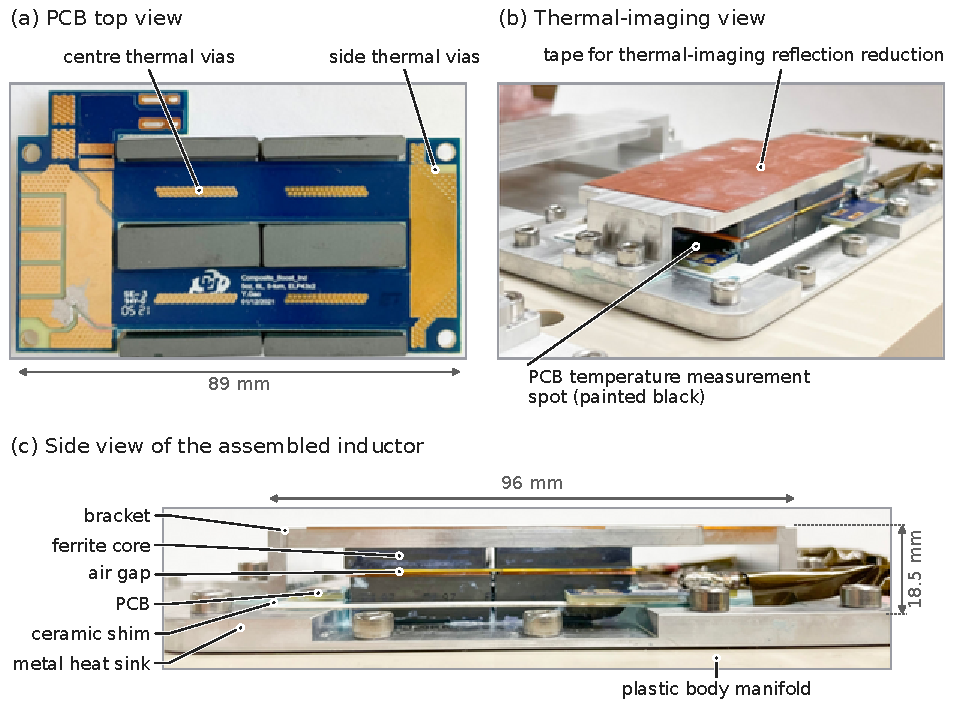
\includegraphics[width=0.75\linewidth]{gao_inductor_prototype}
  \caption[Planar inductor prototype of Gao \emph{et al.}]{Planar inductor
    prototype of Gao \emph{et al.} with an engineered conduction path to the
    cold plate: (a)~PCB top view; (b)~view used for thermal imaging;
    (c)~side view of the assembled inductor. Adapted
    from~\cite{gao_modeling_2022}.}
  \label{fig:gao-inductor}
\end{figure}

\subsection{Form Factor Requirement}
\label{sec:form-factor}

The cooling system must not erode the power density it is meant to enable. With
the magnetic components, heat sinks account for the largest portion of a power
converter's size, and in compact converters the thermal management system can
occupy a large share of the
volume~\cite{biela_cooling_2007,morroni_understanding_2023,friedli_essence_2014}.
Air cooling requires bulky heat sinks, which limited the power density of the
rectifiers of Friedli \emph{et al.}\ (\cref{sec:motivation}). Water cooling is
compact at the device, as the pump and radiator can be placed
remotely~\cite{friedli_essence_2014,laloya_heat_2016}, while phase-change
systems can be smaller and lighter still~\cite{laloya_heat_2016}. For magnetic
components, a compact cooling system must be placed as close as possible to the
windings, typically on both the top and bottom of the
core~\cite{krismer_accurate_2010,biela_cooling_2007}, which places it directly in
the component's leakage field.

\subsection{Efficiency Requirement}
\label{sec:efficiency-req}

To retain the efficiency of the converter, the power drawn by the cooling system,
its burden power, must remain small relative to the power
processed~\cite{laloya_heat_2016}, and the cooling hardware must not introduce
excessive loss into the converter. Single-phase cooling requires fans or pumps,
and raising its heat flux requires narrower channels, which raise the pressure
drop and pumping power steeply~\cite{rahman_emerging_2024,laloya_heat_2016}.
Single-phase cooling therefore trades the maximum temperature it can hold
against the burden power it draws. Phase-change cooling draws little or no
burden power, and is often passive~\cite{laloya_heat_2016}.

Cooling hardware placed near magnetic components, whether single-phase or
phase-change, sits in their leakage field and suffers eddy-current
loss~\cite{biela_cooling_2007,gao_modeling_2022,ouyang_overview_2014}. In Gao
\emph{et al.}'s design, the cold plate and bracket raised the measured AC winding
resistance by \SI{34}{\percent}~\cite{gao_modeling_2022}, and the aluminium
shielding sheet of an IPT pad dissipates about \SI{17}{\watt} in the same way
(\cref{fig:kim-losses})~\cite{kim_thermal_2022}. Biela and Kolar similarly found
that heat-transfer components near an inductor air gap must be recessed from
it~\cite{biela_cooling_2007}. Because magnetic components are present in most
converters~\cite{morroni_understanding_2023}, their leakage fields must be
considered in any PEC cooling design, even where the magnetics are not the main
thermal constraint.

No established scheme therefore meets all three requirements. Phase-change
cooling offers the highest heat flux at low burden power, but is capped by CHF
and offers no control over the temperature swing when passive. Single-phase
cooling is controllable, but its heat flux is bounded by the low thermal
conductivity of air and water, so a higher heat flux costs pumping power. A
coolant with substantially higher thermal conductivity could ease this trade-off
while keeping flow-rate control, which motivates much of the research into
liquid metal coolants~\cite{hodes_potential_2014}.

% ---------------------------------------------------------------------
\section{Liquid Metal as a Coolant}
\label{sec:liquid-metal}

Liquid metals have long been used as coolants where heat fluxes and operating
temperatures exceed those that conventional fluids can tolerate~\cite{rowinski_small_2015}. 
Much of the early characterisation of liquid metal cooling systems was carried out as fundamental research for nuclear
reactors~\cite{rowinski_small_2015}. These systems typically use lead or sodium
coolants, but lead is toxic and requires careful handling and
containment~\cite{oecd_handbook_2015}, whereas sodium is highly chemically
reactive, particularly with water and air, posing fire and explosion
hazards~\cite{foust_sodium-nak_1972}. These factors complicate broader commercial
deployment.

Liquid metal has more recently been proposed as a coolant for computing hardware and
PECs~\cite{fan_ultra-efficient_2026,zhang_water-based_2015}. The driving factor is its high thermal
conductivity, which promises high heat transfer rates~\cite{hodes_potential_2014,fan_ultra-efficient_2026,zhang_experimental_2019,zhang_investigation_2023}.
Such applications typically use gallium (Ga)-based eutectic alloys, the most
common being Galinstan (GaInSn), which is non-toxic and remains liquid at room temperature~\cite{hodes_potential_2014,an_liquid_2024}. 
Galinstan has a thermal conductivity of \SI{16.5}{\watt\per\metre\per\kelvin},
approximately 28 times that of water (\cref{tab:galinstan-properties}), which
enhances heat spreading and reduces temperature gradients~\cite{hodes_potential_2014,zhang_experimental_2019}. 
A Galinstan loop offers single-phase cooling, with no boiling limit to design around, and has the potential to
remove a higher heat flux than water~\cite{hodes_potential_2014, zhang_experimental_2019}.

These benefits come with significant trade-offs (\cref{tab:galinstan-properties}).
High density and viscosity raise pumping power and system weight. Because the
volumetric heat capacity is low, more than twice the flow of water is needed
for the same coolant temperature rise. Electrical conductivity rules out direct
contact with live parts and exposes the coolant to induction heating. 
The wide liquid range, by contrast, removes the CHF limit that
constrains phase-change cooling. The material cost is high, but at the
system level water and Galinstan are comparable because water pumps are
expensive~\cite{fan_ultra-efficient_2026}. Kwon~\cite{kwon_project_2025}
therefore concluded that liquid metal suits specialised applications where
efficiency, compactness and reliability justify its cost.

\begin{table}[htbp]
  \centering
  \caption{Selected properties and cost of the Galinstan used in this work
    (Rich Metals grade EU-10C, 68.5Ga--21.5In--10Sn by
    weight~\cite{noauthor_gainsn_nodate}) relative to water.}
  \label{tab:galinstan-properties}
  \small
  \begin{tabularx}{\linewidth}{@{}>{\raggedright\arraybackslash}p{3.2cm}
      >{\raggedright\arraybackslash}p{2.9cm} L >{\raggedright\arraybackslash}p{1.3cm}@{}}
    \toprule
    Property & Galinstan & Relative to water & Source \\
    \midrule
    Thermal conductivity & \SI{16.5}{\watt\per\metre\per\kelvin} & About 28 times higher & \cite{noauthor_gainsn_nodate} \\
    Density & \SI{6370}{\kilogram\per\metre\cubed} & More than six times higher & \cite{noauthor_gainsn_nodate} \\
    Dynamic viscosity & \SI{2}{\milli\pascal\second} & About 2 times higher & \cite{noauthor_gainsn_nodate} \\
    Specific heat capacity & \SI{366}{\joule\per\kilogram\per\kelvin} & About one-fourteenth & \cite{zhang_experimental_2019} \\
    Volumetric heat capacity & \SI{2.3}{\mega\joule\per\metre\cubed\per\kelvin} & 0.45 times, so about 2.2 times the flow for equal $\Delta T$ & \cite{noauthor_gainsn_nodate} \\
    Electrical conductivity & \SI{3.46e6}{\siemens\per\metre} & Conductor (deionised water: \SI{5.5e-6}{\siemens\per\metre}) & \cite{noauthor_gainsn_nodate} \\
    Melting and boiling points & \SI{10}{\celsius} and above \SI{1300}{\celsius} & Liquid above \SI{10}{\celsius}, so it can solidify in cold storage; boiling will not occur & \cite{noauthor_gainsn_nodate,hodes_potential_2014} \\
    Material cost & US\$200--2000/kg & Orders of magnitude higher & \cite{an_liquid_2024} \\
    \bottomrule
  \end{tabularx}
\end{table}

Much of the reviewed work on Galinstan and other Ga-based coolants focuses on
micro- and mini-channel heat sinks for electronics, typically for heat loads
from watts to hundreds of watts. It is unclear from the literature whether such
systems can be scaled up to the channel sizes and temperatures more typical of
PECs. For example, EV-charging PECs have power classes on the order of tens of
kilowatts for light-duty vehicles and are being standardised up to
\SI{1}{\mega\watt} for heavy-duty
vehicles~\cite{lawton_power_2024,liu_thermal_2025,abb_e-mobility_mcs1200_nodate}. Large liquid
metal systems have been realised for nuclear reactors~\cite{rowinski_small_2015},
but these use different metals, operate at much higher temperatures and are much
larger than even the most powerful PEC applications, although some work has
addressed power electronic
converters~\cite{fan_ultra-efficient_2026,fan_liquid_2021}.

% ---------------------------------------------------------------------
\subsection{Electromagnetic Pumping}
\label{sec:em-pumping}

The low volumetric heat capacity of Galinstan makes pumping demanding. For a
heat load $Q$ and coolant temperature rise $\Delta T$, the required volumetric
flow rate is
\begin{equation}
  \Vdot = \frac{Q}{\rho \, \cp \, \Delta T},
  \label{eq:flow-requirement}
\end{equation}
where $\rho$ is the coolant density and $\cp$ its specific heat capacity.
Galinstan therefore needs about 2.2 times the flow of water
(\cref{tab:galinstan-properties}), which is identified as the primary
bottleneck for liquid metal heat sinks~\cite{hodes_potential_2014,an_liquid_2024}.
Its high thermal conductivity partly offsets this, because it sustains high heat
transfer coefficients in wider channels with a lower pressure
drop~\cite{zhang_water-based_2015,an_liquid_2024}.

The electrical conductivity of Galinstan also allows it to be driven by
electromagnetic (EM) pumps with no moving parts, which are silent,
vibration-free and compact~\cite{hodes_potential_2014}. Previous Part~IV
projects used a permanent-magnet DC conduction
pump~\cite{kwon_project_2025,loh_project_2025}. In this pump, a current $I$
passed through the coolant perpendicular to a magnetic field of flux density
$B$ produces a Lorentz force density
$\mathbf{J}\times\mathbf{B}$~\cite{kwon_project_2025}. An approximation for the
pressure developed is
\begin{equation}
  \Delta p = \frac{B I}{h},
  \label{eq:mhd-pressure}
\end{equation}
where $h$ is the channel height parallel to
$\mathbf{B}$~\cite{loh_project_2025}. Pressure therefore scales directly with
current, so the flow can be modulated to suppress temperature
swing~\cite{an_liquid_2024}, and shallow channels with strong magnets are
favoured. The cost is operation at high current and low voltage
(\SIrange{1}{100}{\ampere}, \SIrange{0.01}{0.5}{\volt},
\SIrange{0.1}{50}{\watt}), with efficiencies of only about
\SIrange{6}{10}{\percent}~\cite{an_liquid_2024,hodes_potential_2014}. Even
so, a conduction pump has drawn less than \SI{15}{\percent} of the power of a
mechanical water pump for the same cooling performance~\cite{an_liquid_2024}.

Induction pumps instead induce current in the coolant through an alternating or
travelling field. They are larger and more complex, but they develop greater
force~\cite{an_liquid_2024}. The field can also come from the converter itself.
Fan \emph{et al.}\ integrated an MHD pump into an inductor, so that the flow
self-adjusts with converter load~\cite{fan_liquid_2021}. The cost is
eddy-current losses in the coolant~\cite{fan_ultra-efficient_2026}. EM pumps
are, however, generally reported as individual designs. Among liquid metal
systems developed for power electronics, only those of Fan
\emph{et al.}\ have been compared against an equivalent water
system~\cite{fan_liquid_2021,fan_ultra-efficient_2026}.

% ---------------------------------------------------------------------
\subsection{Compatibility with Electrical Equipment}
\label{sec:compatibility}

Commercial use of Galinstan raises three concerns: material safety, corrosion
and electromagnetic compatibility. Galinstan was developed as a non-toxic,
non-flammable replacement for mercury. Its negligible vapour pressure means it
poses no inhalation risk~\cite{hodes_potential_2014}. Gallium oxide can damage
the respiratory system at high airborne concentrations, but a closed loop
releases only minimal amounts~\cite{an_liquid_2024}. Prior prototypes managed
skin contact and spillage with gloves, eye protection and containment
trays~\cite{kwon_project_2025,loh_project_2025}.

Ga-based alloys corrode aluminium severely, and copper requires protection
above \SI{100}{\celsius}~\cite{an_liquid_2024}. Erosion at high flow velocities
and the effect on ductile metals remain unstudied~\cite{hodes_potential_2014}.
Plastics and nickel-plated metals~\cite{hodes_potential_2014}, as well as
ceramics such as aluminium nitride~\cite{an_liquid_2024}, are compatible.
Aluminium nitride is also both thermally conductive and electrically
insulating, though expensive~\cite{gao_modeling_2022}.

Electrically, the coolant is a conductor. A leak onto
energised circuitry is a direct short~\cite{hodes_potential_2014}. The loop also
galvanically connects every wetted part, so the EM pump supply can energise the
radiator and cold plate~\cite{kwon_project_2025}. There is also potential for nearby
magnetics to induce eddy currents in the coolant, though this has not been strictly explored in the literature
(\cref{sec:thermal-management})~\cite{an_liquid_2024, fan_ultra-efficient_2026}.
As a result, low-cost plastic piping suits low-field regions. 
Near magnetics, it may be preferable to shield the coolant with a more conductive material to reduce eddy losses.

% ---------------------------------------------------------------------
\section{Research Gap and Objectives}
\label{sec:research-gap}

\subsection{Research Gap}
\edited{Trimmed only. The two opening sentences (water cooling is bounded by
water's thermal conductivity; Galinstan's higher conductivity can improve heat
transfer, both cited to Hodes \emph{et al.}) repeated
\cref{sec:thermal-management,sec:liquid-metal} and were cut. The two closing
sentences of the second gap (most converters contain magnetics; a cooling
system that does not cool them must still tolerate their leakage fields) are
now made in \cref{sec:thermal-management} and are replaced by a back-reference.
In the first gap, ``which use different metals at much higher temperatures''
was cut, as \cref{sec:liquid-metal} already says so.}

This study aims to address two gaps identified in the literature.

The first is the lack of comparisons between water and liquid metal at the scale
of a converter's cooling loop. Most existing comparisons are made for micro- and
mini-channel heat
sinks~\cite{hodes_potential_2014,zhang_water-based_2015,zhang_experimental_2019,an_liquid_2024},
or lie at the scale of nuclear reactors~\cite{rowinski_small_2015}. This study
aims to quantify the
trade-offs of the Galinstan system (as designed
in~\cite{kwon_project_2025,loh_project_2025}) relative to a comparable water-cooling
system.

The second is the cooling of magnetic components with Galinstan. To the author's
knowledge, no study has demonstrated Galinstan cooling of a magnetic component,
such as a power-dense inductor, or quantified the eddy-current losses induced in
the coolant by its leakage field. Eddy-current losses have been assessed in AC
conduction pumps~\cite{fan_ultra-efficient_2026}, and an inductor has been used to drive a
pump~\cite{fan_ultra-efficient_2026,fan_liquid_2021}, but not to cool the inductor itself
directly. As argued in \cref{sec:thermal-management}, the coolant's loss in a
leakage field matters even where the coolant does not cool the magnetics.

This project addresses both gaps using the existing Galinstan loop of
Loh~\cite{loh_project_2025} and Kwon~\cite{kwon_project_2025}. The loop comprises a
permanent-magnet MHD pump, perfluoroalkoxy (PFA) tubing, a cold plate and a
fan-cooled radiator, and can remove up to a \SI{72}{\watt} resistive
load~\cite{kwon_project_2025,loh_project_2025}. The loop was not tested against water
in the same apparatus, and its experiments did not consider magnetics:
Loh~\cite{loh_project_2025} focused on switching devices because Galinstan was
unlikely to interfere with them, unlike magnetics, and Kwon~\cite{kwon_project_2025}
excluded direct integration and testing with magnetics because of time
limitations and uncertainty about electromagnetic interference. Both recommended
comparison with water cooling, and Kwon also recommended testing higher heat
loads and investigating the interaction with inductive pad
fields~\cite{kwon_project_2025,loh_project_2025}.
\edited{``This project was not tested against water'' referred to the previous
project's loop, not this project; reworded to ``The loop was not tested
\dots''.}

\subsection{Research Questions}
\label{sec:research-questions}

These gaps lead to two research questions.

\begin{description}[leftmargin=3.2em,labelwidth=2.6em,labelsep=0.6em,itemsep=4pt]
    \item[RQ1] At the same heat load, how do the thermal resistance and pumping
    power of the Galinstan loop compare with those of a similar conventional
    water loop?
    \item[H1] Galinstan's higher thermal conductivity will lower the convective
    resistance relative to water in the same cold plate. However, the total
    thermal resistance of the Galinstan loop will be higher than that of the
    water loop. Its low volumetric heat capacity and low flow rate give a
    caloric resistance comparable to the conduction resistance of the cold
    plate.
    \item[RQ2] Can the Galinstan loop cool a power-dense inductor while adding
    minimal loss to the existing aluminium cold plate, and how large is the
    eddy-current loss induced in the coolant?
    \item[H2] The Galinstan loop will have a cooling effect on the inductor above that of natural convection. 
    The increase in loss due to eddy-current loss induced in the coolant will be
    small compared to the loss of introducing the cold plate.
    The metal of the cold plate between the inductor and the coolant is
    several skin depths thick at \SI{85}{\kilo\hertz}. Additionally, the high-frequency field will not change the coolant flow
    measurably. 
\end{description}

% =====================================================================
%  Chapter 3 -- Methodology
%  Structure follows the Experimental Section of Kwon (2025): setup,
%  design, modelling, then the experimental procedure.
% =====================================================================
\chapter{Methodology}
\label{ch:experimental}

The following sections detail the methodology used to evaluate
magnetohydrodynamically pumped Galinstan as a coolant for PECs. Two objectives
guided the work. The first is to compare the thermal performance of the
Galinstan cooling loop with that of a similar water cooling loop under
equivalent operating conditions (RQ1). The second is to quantify the influence
of a high-frequency magnetic leakage field on the Galinstan coolant (RQ2).
\Cref{sec:setup} describes the experimental setup, including the two cooling
loops, the instrumentation and the safety considerations.
\Cref{sec:inductor-design} presents the design of the power-dense inductor used
as the heat source in the second experiment. \Cref{sec:thermal-model} develops
the thermal models used to interpret the measurements, and
\cref{sec:programme} gives the procedures for the two experiments.

% ---------------------------------------------------------------------
\section{Experimental Setup}
\label{sec:setup}

\subsection{Cooling System Overview}
\label{sec:loop-overview}

Two cooling loops were used in this project, one circulating Galinstan and the
other water. Both follow the arrangement shown in \cref{fig:cooling-loop}. A
pump drives the coolant through a cold plate that interfaces with the heat
source, and then through a fan-cooled radiator, where the heat is rejected to
the environment. A flow sensor in the hot line measures the coolant flow rate.

\begin{figure}[htbp]
  \centering
  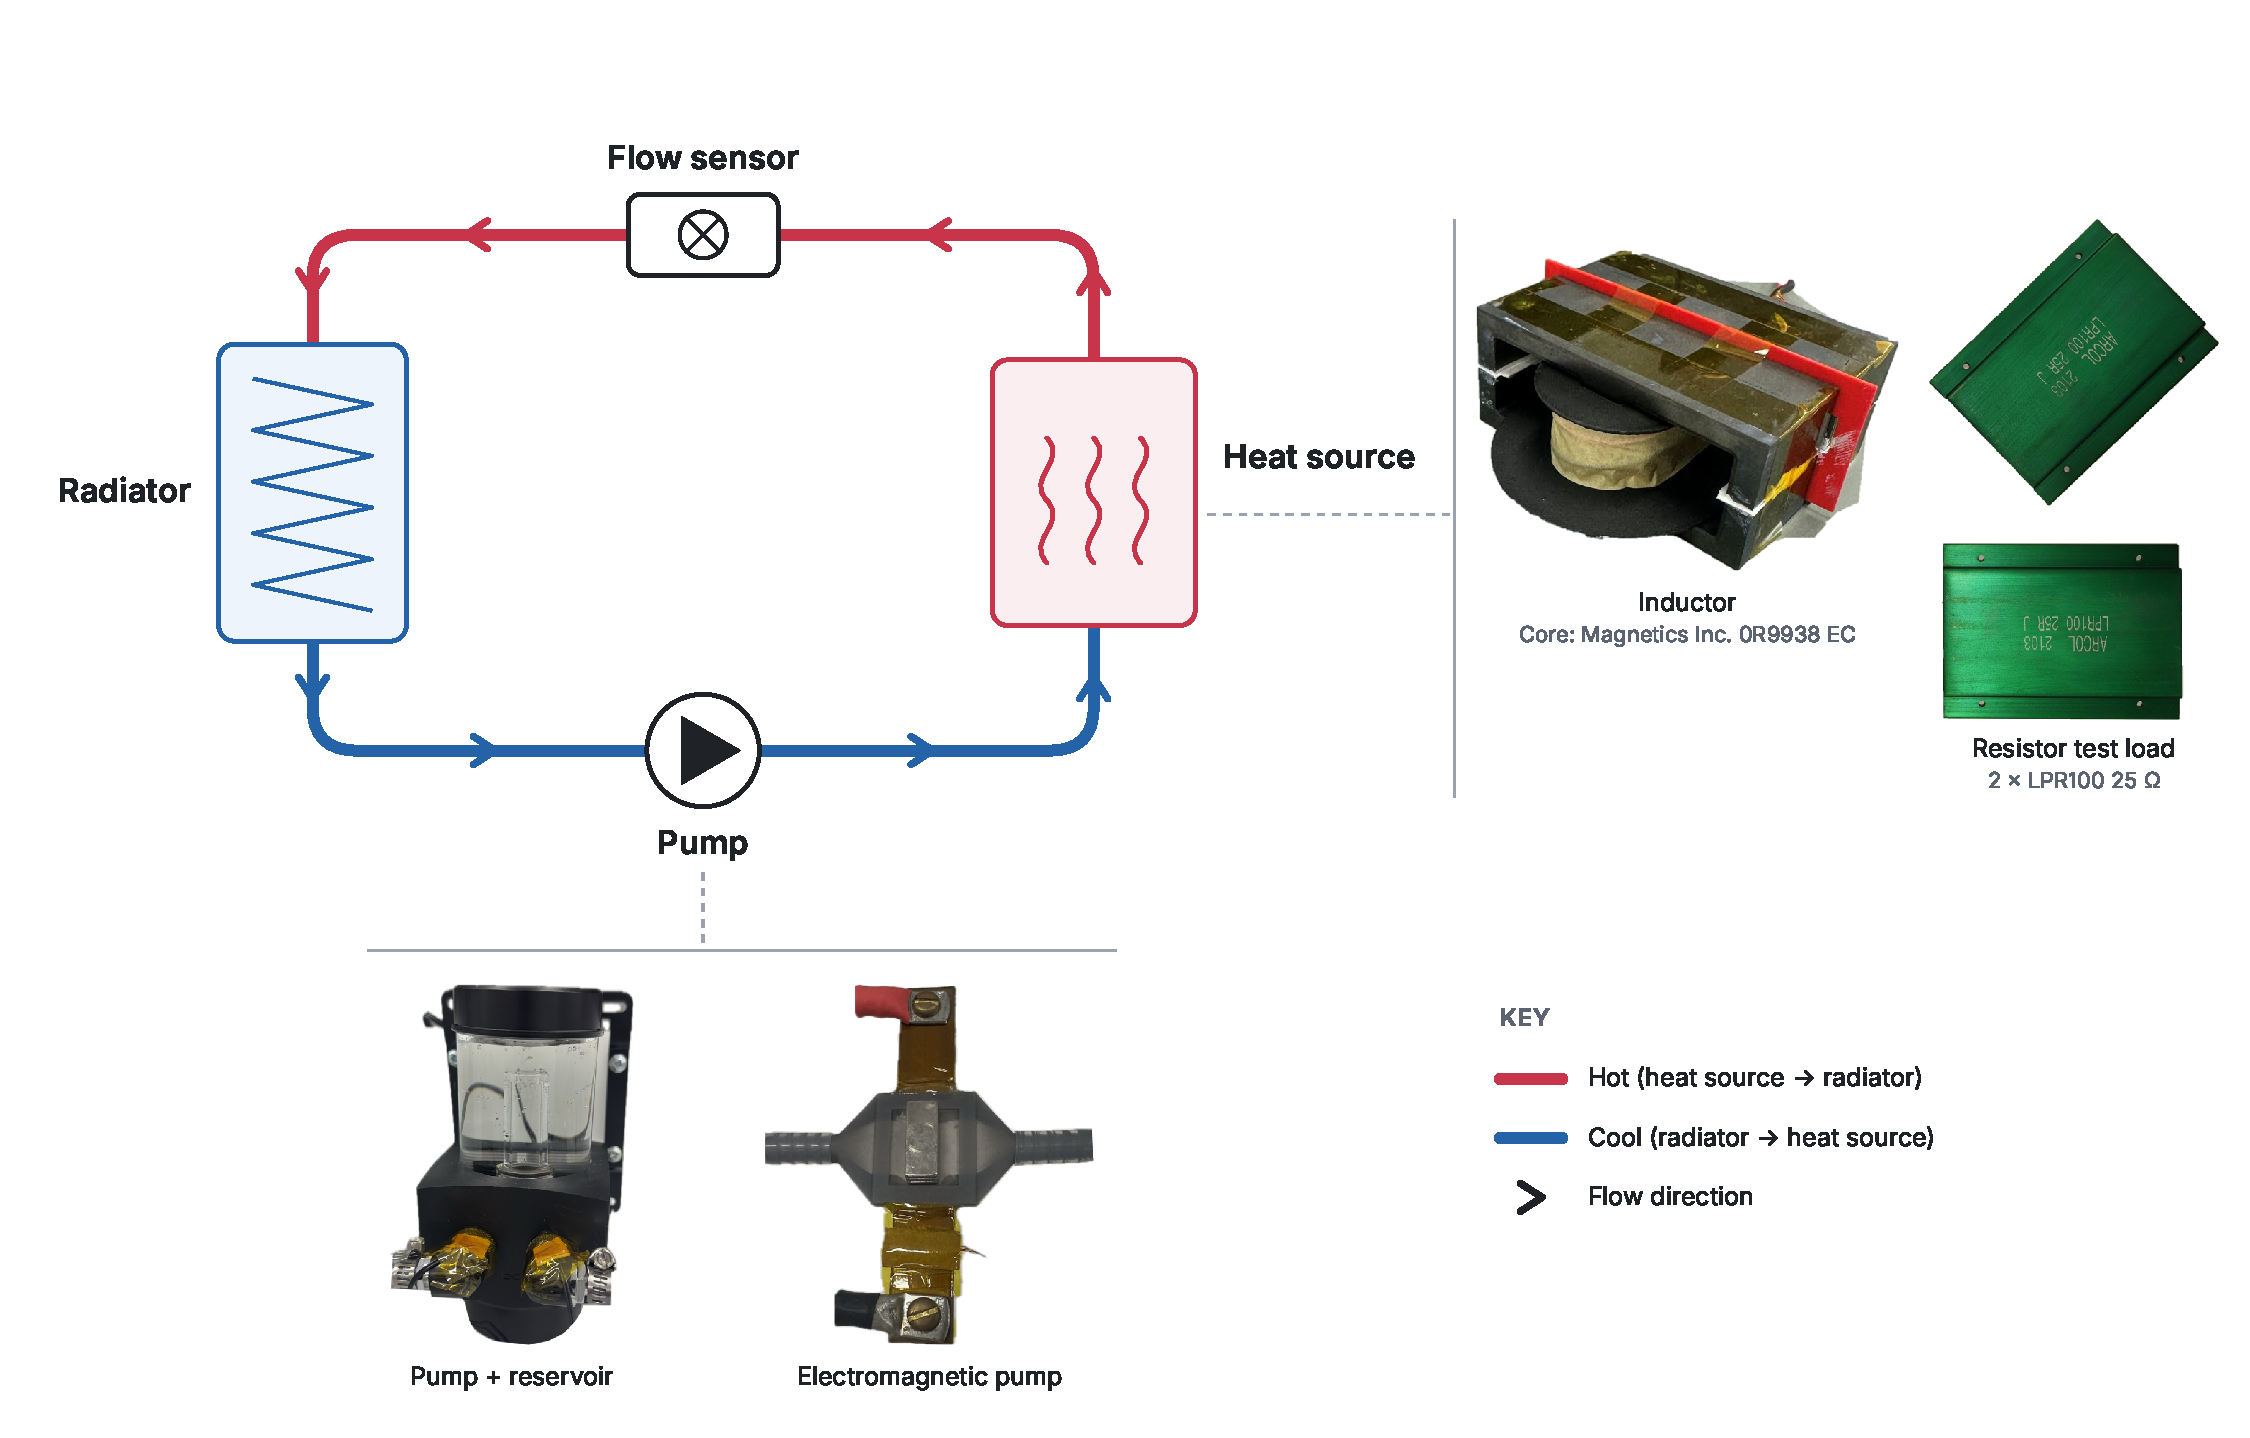
\includegraphics[width=0.85\linewidth]{figures/cooling_loop.pdf}
  \caption{Cooling loop arrangement shared by the Galinstan and water systems.
    The coolant is pumped through the heat source (resistor test load or
    inductor), past the flow sensor and through the radiator before returning
    to the pump. The water loop uses a pump with an integrated reservoir; the
    Galinstan loop uses an electromagnetic pump.}
  \label{fig:cooling-loop}
\end{figure}

The Galinstan loop is the apparatus constructed by the 2025 Part~IV Project~\#51
group~\cite{kwon_project_2025,loh_project_2025}. Galinstan is circulated by a
permanent-magnet DC conduction pump, in which a current passed through the
coolant between two copper electrodes produces a Lorentz force
(\cref{sec:em-pumping}). The pump is supplied by a XANTREX XKW~60--18 DC power
supply, which provides up to \SI{18}{\ampere}. PFA tubing carries the coolant
to an ATS-TCP-1001 tubed cold plate and back through an ATS-TCP-1003 cold plate
fitted with a heat sink and two fans, which acts as the
radiator~\cite{kwon_project_2025,advanced_thermal_solutions_inc_tubed_2021}.
Conventional mechanical flow meters are not compatible with Galinstan, so the
flow rate is measured with an electromagnetic flow sensor of the same
construction as the pump. The flowing coolant induces an EMF $E$ across the
sensor electrodes, from which the volumetric flow rate is $\Vdot = Eh/B$, where
$h$ is the channel height and $B$ the magnetic flux density across the
channel~\cite{kwon_project_2025}.

The water loop was designed and built by the project partner, Ekbote, to
replicate the Galinstan apparatus, and its design is detailed in Ekbote's
project report~\cite{ekbote_project_2026}. It uses the same model of tubed cold
plate (ATS-TCP-1001), so that the two
coolants are compared through an identical cold-plate geometry
(\cref{tab:coolant-properties}). The water is circulated by a pump with an
integrated reservoir, whose speed is set by the duty cycle of its drive signal,
and the flow rate is read directly from a Sea Zhongjiang digital flow meter. A
valve was later added to the water loop to reduce the flow below the
controllable range of the pump. The two loops therefore share the heat source
and the cold-plate geometry, but differ in the pump, the achievable flow range
and the method of flow measurement.

\subsection{Heat Sources}
\label{sec:heat-sources}

Two heat sources were used. For the first experiment, heat was applied by two
\SI{100}{\watt}, \SI{25}{\ohm} ARCOL LPR100 resistors mounted side by side on the
cold plate with a thermal interface material. The resistors were connected in
series and supplied by a GW Instek GPE-3323 DC power supply, so that the
dissipated power could be read directly from the supply. A heat load of
\SI{72}{\watt} (\SI{60}{\volt} across the \SI{50}{\ohm} pair) was used for most
tests, the same load used in~\cite{kwon_project_2025,loh_project_2025}. The
resistors were covered with polystyrene insulation to reduce the heat lost to
the environment. For the second experiment, the resistors were replaced by a
power-dense planar inductor, whose design is described in
\cref{sec:inductor-design}.

\subsection{Instrumentation}
\label{sec:instrumentation}

Galinstan is corrosive to many commonly used sensor materials, which restricts
the range of compatible measurement devices (\cref{sec:compatibility}). System
performance was therefore evaluated using the limited set of measurements
summarised in \cref{tab:measurements}. Temperatures around each loop were
logged continuously by a thermistor data-acquisition system adapted
from~\cite{kwon_project_2025,loh_project_2025}. At steady state, K-type
thermocouples, with an accuracy of $\pm\SI{2.2}{\celsius}$~\cite{loh_project_2025},
were used as the reference temperatures at the resistor, the cold-plate inlet
and the cold-plate outlet. A thermal camera was used where available, chiefly
for the inductor experiment.

\begin{table}[htbp]
  \centering
  \caption{Measured quantities and instrumentation.}
  \label{tab:measurements}
  \small
  \begin{tabularx}{\linewidth}{@{}>{\raggedright\arraybackslash}p{2.7cm}
      >{\raggedright\arraybackslash}p{4.1cm} L@{}}
    \toprule
    Quantity & Description & Method \\
    \midrule
    \multirow[t]{2}{=}{Heat load}
      & Power dissipated by the resistors.
      & Read from the GW Instek GPE-3323 DC power supply. \\
      & Power dissipated in the inductor.
      & Estimated from the core-loss model and the measured AC resistance
        (\cref{sec:model-validation}). \\
    \midrule
    \multirow[t]{2}{=}{Volumetric flow rate, $\Vdot$}
      & Galinstan loop.
      & EMF $E$ of the electromagnetic flow sensor, read with an Agilent 34410A
        digital multimeter; $\Vdot = Eh/B$~\cite{kwon_project_2025}. \\
      & Water loop.
      & Read directly from the Sea Zhongjiang digital flow meter. \\
    \midrule
    Temperature
      & Thermistors around the loop and, at steady state, thermocouples at the
        resistor, cold-plate inlet and cold-plate outlet.
      & Data-acquisition system adapted from~\cite{kwon_project_2025,loh_project_2025};
        thermal camera where available. \\
    \midrule
    Pump power
      & Electrical input power to each pump.
      & Voltage across the pump terminals and current from each pump's DC
        power supply. \\
    \midrule
    AC resistance, $R_{\mathrm{ac}}$
      & Series resistance of the inductor winding.
      & Agilent E4980A LCR meter (\cref{sec:exp2}). \\
    \midrule
    Pump volume
      & Volume occupied by each pump.
      & Physical measurement, supplemented by CAD dimensions where physical
        measurement is impractical. \\
    \bottomrule
  \end{tabularx}
\end{table}

\subsection{Safety Considerations}
\label{sec:safety}

The safety of project members and other laboratory users was prioritised
throughout the experimental setup and operation. Every experiment was set up by
two project members, and all connections were cross-checked with the project
partner before the system was energised. While temperatures exceeded
\SI{38}{\celsius}, the apparatus was continuously monitored by at least one
project member, and no one was permitted to interact with the system while it
was live. All electrical terminals operating above \SI{50}{\volt} DC were
covered, and the inverter and resonant tank used in the second experiment were
fully enclosed in acrylic boxes. Protective eyewear was worn, and physical
barriers prevented accidental contact with the live system. At shutdown, the
heat source was switched off first while the coolant continued to circulate,
and the apparatus was supervised for at least 30 minutes, until it had cooled
below \SI{38}{\celsius}.

% ---------------------------------------------------------------------
\section{Inductor Design}
\label{sec:inductor-design}

Cooling systems for magnetic components sit in their leakage fields
(\cref{sec:form-factor}), which could heat a Galinstan coolant. An initial ANSYS
simulation, with the Galinstan modelled as a stationary solid, found it 3.2
times as lossy as aluminium and almost 3.9 times as lossy as copper, and showed
that \SI{1}{\milli\metre} of copper shielding reduced the total loss by over
\SI{70}{\percent}. To measure this effect, a power-dense inductor that requires
active cooling was built and placed on the Galinstan cold plate. It operates at
\SI{85}{\kilo\hertz}~\cite{society_of_automotive_engineers_r_2024}, so that its
leakage field is representative of IPT magnetics (\cref{sec:ipt-losses}), and
uses a planar geometry, which offers better thermal performance than
alternatives such as pot cores. The final construction is shown in
\cref{fig:inductor-photo}.

\subsection{Analytical and Numerical Design}
\label{sec:analytical-design}

To reduce computation time and narrow the design space, an analytical model was
developed before the numerical simulations. This initial model assumed a
two-part construction of TDK N85 ferrite ELP-type cores, and swept the air-gap
length (\SIrange{0.5}{1.5}{\milli\metre}) and the number of turns (8--12). The
core loss of each design was estimated with the Steinmetz equation, which
expresses the loss per unit volume as a power law in frequency and peak flux
density~\cite{li_review_2022}. The model identified designs whose loss exceeds
the core's datasheet loss limit of
\SI{17.88}{\watt}~\cite{magnetics_inc_specification_2005}, so that active
cooling is required, while keeping the peak flux density below about
\SI{300}{\milli\tesla}.

An ANSYS model was then constructed and run as a two-parameter sweep over
air-gap length and number of turns. It was later found that the available cores
were Magnetics Inc.\ Material~R rather than the assumed TDK N85. A custom
material definition was therefore created by modifying the properties of TDK
N95, which are similar to those of Material~R. The core material was assumed to
operate at \SI{65}{\celsius}, the target steady-state operating temperature for
the experiments. With the material defined, a parameter sweep (8--12 turns,
\SIrange{0.5}{1.2}{\milli\metre} air gap) was performed to extract the
inductance and core loss.

To finalise the design, the flux density in the core was checked and found to
be acceptable, within the linear region of operation (\cref{fig:flux-density}).
The final design parameters, including the inductance and core loss of the
chosen design, are given in \cref{tab:inductor-design}.

\begin{figure}[htbp]
  \centering
  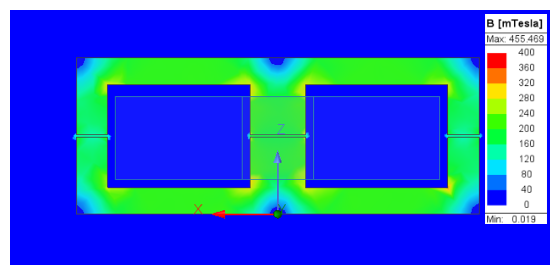
\includegraphics[width=0.72\linewidth]{inductor_flux_density}
  \caption{Magnetic flux density in the selected inductor design ($N = 8$,
    $l_{\mathrm{g}} = \SI{0.6}{\milli\metre}$).}
  \label{fig:flux-density}
\end{figure}

\begin{table}[htbp]
  \centering
  \caption{Final inductor parameters from the ANSYS model at the rated current
    of \SI{12}{\ampere} rms.}
  \label{tab:inductor-design}
  \begin{tabular}{@{}lll@{}}
    \toprule
    Parameter & Value & Unit \\
    \midrule
    Core geometry  & Magnetics Inc.\ 0\,9938\,EC & -- \\
    Core material  & Magnetics Inc.\ Material~R  & -- \\
    Air-gap length & 0.6   & \si{\milli\metre} \\
    Turns          & 8     & -- \\
    Inductance     & 92.5  & \si{\micro\henry} \\
    Core loss      & 30.81 & \si{\watt} \\
    \bottomrule
  \end{tabular}
\end{table}

\subsection{Model Validation}
\label{sec:model-validation}

Once the inductor had been built (\cref{fig:inductor-photo}), measurements were
taken to design the LCC tuning required to drive the desired resonant current.
These measurements also serve to validate the model, whose values at the rated
current of \SI{12}{\ampere} rms are given in \cref{tab:inductor-design}.

\begin{figure}[htbp]
  \centering
  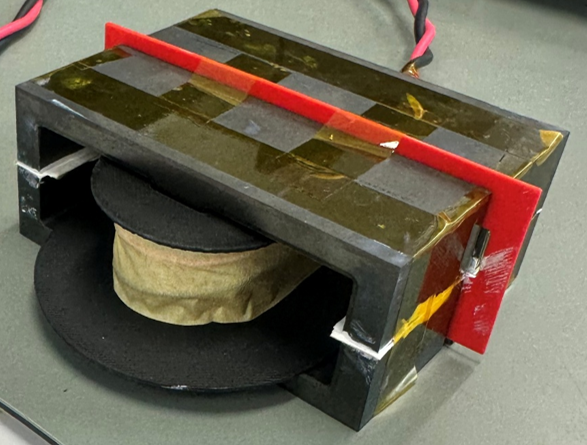
\includegraphics[width=0.42\linewidth]{inductor_photo}
  \caption{Constructed planar inductor.}
  \label{fig:inductor-photo}
\end{figure}

The inductance was measured as \SI{92.1}{\micro\henry}, within \SI{1}{\percent}
of the simulation model, although this measurement included the effect of long
leads, which would be expected to increase it. The AC resistance
$R_{\mathrm{ac}}$, which determines the winding loss, was measured with an LCR
meter at low excitation as \SI{83}{\milli\ohm}, giving a winding loss of
\SI{11.95}{\watt} at \SI{12}{\ampere} rms.

For a heat transfer investigation in which temperatures are continuously
monitored, some uncertainty in the loss estimate is acceptable. For the later
experiments, the total inductor loss is therefore taken as \SI{42.76}{\watt}
(\SI{30.81}{\watt} core loss plus \SI{11.95}{\watt} winding loss).

\subsection{Thermal Considerations and Cooling Strategy}
\label{sec:inductor-thermal}

The main constraint was asymmetric cooling. The upper core relies on convection
to ambient air, while the lower core sits on the cold plate, and the air gap
between them acts as a thermal insulator. Thermal paste was applied between the
upper and lower cores to reduce the temperature difference and improve heat
transfer to the cooling system. Although not optimal, this configuration is
suitable for the second experiment, which aims to demonstrate Galinstan cooling
of a power-dense inductor and to assess the leakage-field interaction rather
than to produce the best-performing system. Future work could improve the design
by cooling both the top and bottom cores, or by using asymmetric core designs
with an integrated heat-transfer path, such as the inductor of Gao
\emph{et al.}~\cite{gao_modeling_2022}.

\subsection{Capacitor Tuning}
\label{sec:capacitor-tuning}

The allowable reactance of the inductor was limited by the maximum voltage
developed across the series tuning capacitors needed to boost the volt-amperes
(VA) in the inductor, which was limited to \SI{150}{\volt} across any single
capacitor. To find
acceptable tuning values, an optimisation model was developed using the Solver
add-in in Microsoft Excel, which made it possible to check quickly whether a
given inductance was feasible or would cause the capacitor voltage to exceed its
rating.

The target capacitance is given by
\begin{equation}
  C_{\mathrm{target}} = \frac{1}{2\pi f \left(2\pi f L_{1} - X_{\mathrm{res}}\right)},
  \label{eq:c-target}
\end{equation}
where $f$ is the resonant frequency of the network (\SI{85}{\kilo\hertz}),
$L_{1}$ is the inductance of the primary magnetics and $X_{\mathrm{res}}$ is the
resonant reactance of the system. $X_{\mathrm{res}}$ sets the resonant current in
the primary magnetics, as given by
\begin{equation}
  X_{\mathrm{res}} = \frac{2\sqrt{2}\, V_{\mathrm{DC}}}{\pi I_{1}},
  \label{eq:x-res}
\end{equation}
where $I_{1}$ is the desired resonant current and $V_{\mathrm{DC}}$ is the DC bus
voltage, here \SI{60}{\volt}. \Cref{eq:x-res} is valid only for a conduction
angle of \SI{180}{\degree}. With the measured inductance of \SI{92.1}{\micro\henry} and a resonant current of
\SI{12}{\ampere}, \cref{eq:c-target,eq:x-res} give a target capacitance of
\SI{41.90}{\nano\farad}.

Initially, the optimisation model selected a single capacitor value for the
entire board. The result was relatively poor, with the best design differing by
\SI{8.11}{\percent} from the target capacitance. The model was then extended to
allow one value from a limited set (\SIlist{22;68;100}{\nano\farad}) to be
selected for each of the four series-connected rows of the tuning board, with up
to 14 capacitors in parallel per row. This reduced the detuning to
\SI{2.12}{\percent} of the target value. The final arrangement, with the voltage
across each row at the rated current, is given in \cref{tab:capacitor-opt}. The
highest row voltage is about \SI{146}{\volt}, within the \SI{150}{\volt} limit.

\begin{table}[htbp]
  \centering
  \caption{Final arrangement of the series tuning capacitors from the
    optimisation model. The four rows are connected in series; row voltages are
    at \SI{12}{\ampere} rms and \SI{85}{\kilo\hertz}.}
  \label{tab:capacitor-opt}
  \small
  \begin{tabular}{@{}lcccc@{}}
    \toprule
    Row & Capacitor value & Number in parallel & Row capacitance & Row voltage \\
        & (\si{\nano\farad}) & & (\si{\nano\farad}) & (\si{\volt}) \\
    \midrule
    1 & 22 & 7 & 154 & 145.9 \\
    2 & 68 & 3 & 204 & 110.1 \\
    3 & 22 & 7 & 154 & 145.9 \\
    4 & 22 & 7 & 154 & 145.9 \\
    \midrule
    \multicolumn{3}{@{}l}{Target capacitance}   & 41.90 & \\
    \multicolumn{3}{@{}l}{Achieved capacitance} & 41.01 & \\
    \multicolumn{3}{@{}l}{Error}                & 0.89 (\SI{2.12}{\percent}) & \\
    \bottomrule
  \end{tabular}
\end{table}

% ---------------------------------------------------------------------
\section{Thermal Modelling}
\label{sec:thermal-model}

Thermal models were developed alongside the experiments, both to interpret the
measurements and to extend them beyond the conditions the apparatus could reach.
This section first presents a lumped thermal network and the $\varepsilon$--NTU
analysis used to calculate its cold-plate resistance, followed by the convection
correlations and test conditions it relies on. A conjugate heat transfer
simulation, which resolves the temperature field that the network lumps
together, is then described. The models are compared with the measurements in
\cref{ch:results}.

\subsection{Thermal Network}
\label{sec:thermal-network}

Following the analyses of Kwon~\cite{kwon_project_2025} and
Loh~\cite{loh_project_2025}, the input heat $\Qin$ divides at the resistor node
$\Tres$, as shown in \cref{fig:thermal-network}. Part of the heat is
lost to ambient through $\Rmisc$. The rest, $\Qplate$, passes through the
package resistance $\Rpack$ (resistor and thermal interface) to a fictitious
isothermal plate node $T_{\mathrm{P}}$, and then through the cold-plate
resistance $\Rcp$ to the coolant inlet:
\begin{equation}
  \Qin = \frac{\Tres - T_{\mathrm{A}}}{\Rmisc}
       + \frac{\Tres - \Tin}{\Rpack + \Rcp}.
  \label{eq:network}
\end{equation}
The resistance to ambient $\Rmisc$ was found for each loop from a no-flow test
at a heat load of \SI{12}{\watt}. With no coolant flow, the heat input is lost
to the environment, so
\begin{equation}
  \Rmisc = \frac{\Tres - T_{\mathrm{A}}}{\Qin}.
  \label{eq:rmisc}
\end{equation}
This resistance was then used to calculate the loss to the environment at any
resistor temperature. For the Galinstan loop, $T_{\mathrm{A}} =
\SI{20.5}{\celsius}$ and $\Rmisc = \SI{3.33}{\celsius\per\watt}$; for the water
loop, $T_{\mathrm{A}} = \SI{21.6}{\celsius}$ and
$\Rmisc = \SI{2.95}{\celsius\per\watt}$. With these values, between
\SI{9}{\watt} and \SI{12}{\watt} of the heat load is lost to the environment in
each test (\cref{tab:measured-performance}). This network was used in all the
following models.
\issue{\Cref{fig:thermal-network} still labels the resistor node
$T_{\mathrm{M}}$; update the image to $T_{\mathrm{resistor}}$.}

\begin{figure}[htbp]
  \centering
  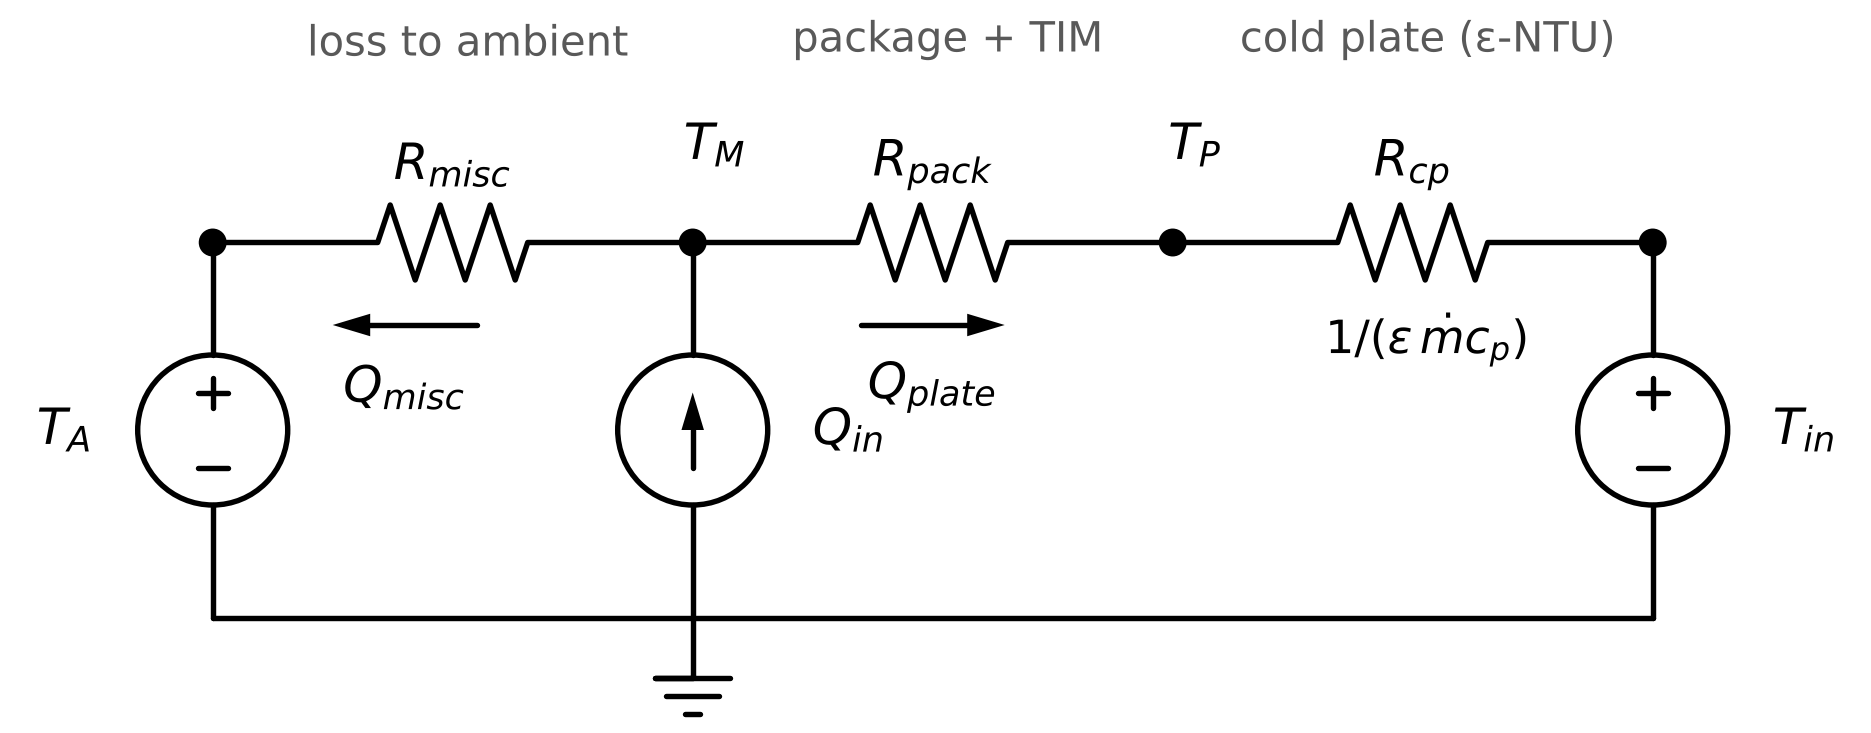
\includegraphics[width=0.85\linewidth]{thermal_network}
  \caption{Thermal network as an electrical analogue (temperature $\equiv$
    potential, heat flow $\equiv$ current); $T_{\mathrm{A}}$ and $\Tin$ are fixed
    boundary conditions.}
  \label{fig:thermal-network}
\end{figure}

\subsection{\texorpdfstring{$\varepsilon$--NTU}{epsilon-NTU} Analysis of the Cold Plate}
\label{sec:eps-ntu}

For this analysis, the plate is considered isothermal at $T_{\mathrm{P}}$, so
coolant entering at $\Tin$ approaches the plate temperature exponentially. An
energy balance on a tube element of perimeter $P$ gives~\cite{bergman_fundamentals_2017}
\begin{equation}
  \frac{T_{\mathrm{P}} - T_{\mathrm{f}}(x)}{T_{\mathrm{P}} - \Tin}
    = \exp\!\left(-\frac{hPx}{\mdot\,\cp}\right).
  \label{eq:temp-profile}
\end{equation}
At the outlet ($x = L$, $PL = A$), the exponent is defined as the number of
transfer units, $\NTU = hA/(\mdot\,\cp)$. This is the ratio of the
wall-to-coolant convective conductance to the heat-capacity rate of the coolant.
Each transfer unit reduces the remaining plate-to-coolant temperature difference
by a factor of $e$, so the coolant absorbs about \SI{63}{\percent} of the maximum
possible heat after one transfer unit~\cite{bergman_fundamentals_2017}. Defining
the effectiveness $\varepsilon$ as this fraction gives
\begin{equation}
  \Qplate = \varepsilon\,\mdot\,\cp\,(T_{\mathrm{P}} - \Tin), \qquad
  \varepsilon = 1 - e^{-\NTU}, \qquad
  \Rcp = \frac{1}{\varepsilon\,\mdot\,\cp},
  \label{eq:effectiveness}
\end{equation}
\begin{equation}
  T_{\mathrm{P}} = \Tin + \Qplate\Rcp, \qquad
  \Tout = \Tin + \frac{\Qplate}{\mdot\,\cp}.
  \label{eq:plate-outlet}
\end{equation}
This is the effectiveness relation for one flow stream against an isothermal
surface~\cite{bergman_fundamentals_2017}. Its limits show whether a coolant is
limited by convection at the wall or by its ability to transport heat
(caloric-limited), as summarised in \cref{tab:ntu-regimes}.

\begin{table}[htbp]
  \centering
  \caption{Limiting regimes of the $\varepsilon$--NTU relation for an isothermal
    plate.}
  \label{tab:ntu-regimes}
  \small
  \begin{tabular}{@{}lllll@{}}
    \toprule
    Regime & NTU & $\varepsilon$ & $\Rcp$ & Lever to reduce $\Rcp$ \\
    \midrule
    Convection-limited & $\ll 1$ & $\approx \NTU$ &
      $\approx 1/(hA) + 1/(2\mdot\,\cp)$ & Raise $hA$ (Nu, area) \\
    Transitional & $\approx 1$ & $1 - e^{-\NTU}$ &
      $1/(\varepsilon\,\mdot\,\cp)$ & Both \\
    Caloric-limited & $\gg 1$ ($\gtrsim 3$) & $\to 1$ &
      $\to 1/(\mdot\,\cp)$ & Raise $\mdot\,\cp$ (flow rate) \\
    \bottomrule
  \end{tabular}
\end{table}

The isothermal-plate assumption relies on in-plane heat spreading within the
\SI{15}{\milli\metre} 6063 aluminium base (\cref{fig:coldplate-heatflow}). The
assumption weakens as the coolant temperature rise between inlet and outlet,
$\Delta T_{\mathrm{cool}} = \Qplate/(\mdot\,\cp)$, increases. The predicted rise
is below \SI{2}{\celsius} for water but approximately
\SIrange{17}{20}{\celsius} for Galinstan, so the model is expected to describe
water better than Galinstan. For this reason, the package resistance $\Rpack$
was calibrated on the two turbulent water tests, which give the most nearly
isothermal plate, as \SI{0.242}{\celsius\per\watt}. It was then held at this
value for all flows and both coolants.

\begin{figure}[htbp]
  \centering
  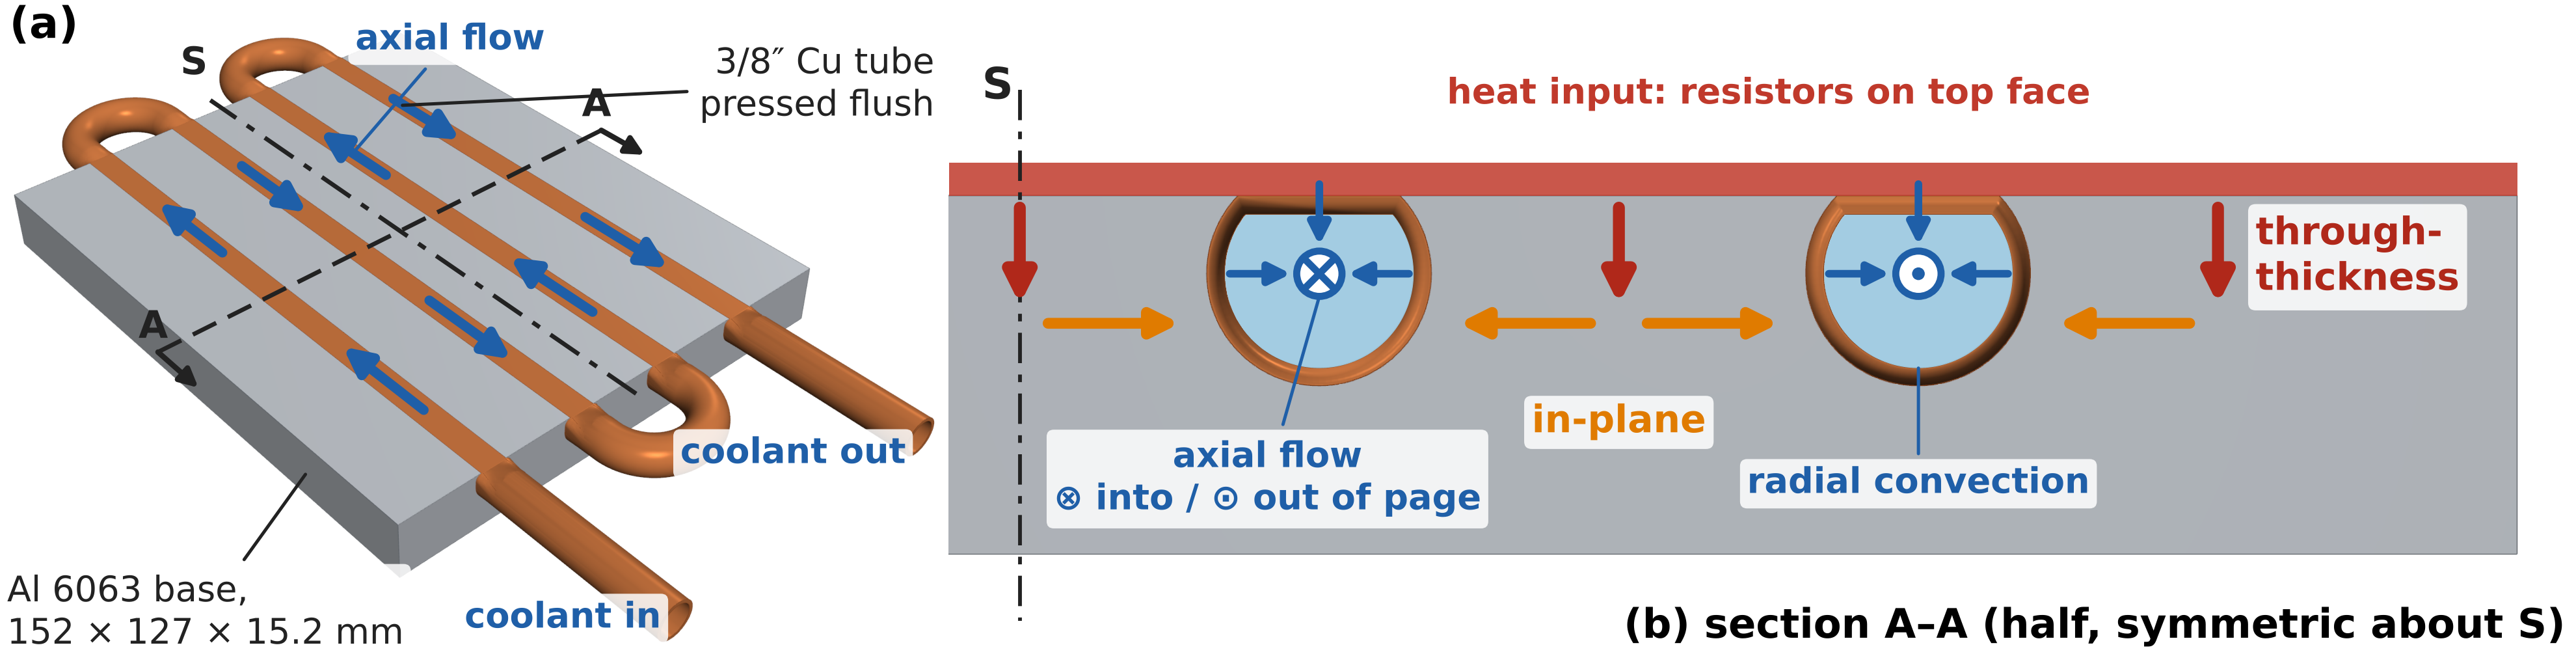
\includegraphics[width=0.85\linewidth]{coldplate_heat_flow}
  \caption{Heat-flow directions in the cold plate: in-plane spreading (plate),
    through-thickness conduction (part of $\Rpack$), axial flow and radial
    convection ($R_{\mathrm{conv}}$).}
  \label{fig:coldplate-heatflow}
\end{figure}

\subsection{Convection Correlations and Test Conditions}
\label{sec:convection}

The $\varepsilon$--NTU model requires an estimate of the heat transfer
coefficient $h$ between the tube wall and the coolant. It is obtained from
standard correlations for the Nusselt number, $\mathrm{Nu} = hD/k$, a
dimensionless measure of how effectively the flowing coolant removes heat from
the wall. For laminar flow, the Shah and London
correlation~\cite{shah_laminar_1978} gives the mean Nu along a tube at constant
wall temperature, including the thermal entry region where heat transfer is
highest. It is applied to each \SI{152}{\milli\metre} pass separately, on the
assumption that the U-bends mix the flow. For turbulent water
($\mathrm{Re} \geq 4000$), Gnielinski's correlation~\cite{bergman_fundamentals_2017}
is used, and no estimate is made in the transitional range
$2300 < \mathrm{Re} < 4000$. Galinstan remains laminar up to
\SI{5}{\milli\litre\per\second} ($\mathrm{Re} \leq 2110$). The correlations and
worked calculations for both coolants are given in \cref{app:convection}.

The NTU analysis uses these correlations for both coolants. For the turbulent
water tests, however, the cold-plate resistance given in the ATS-TCP-1001
datasheet~\cite{advanced_thermal_solutions_inc_tubed_2021} was later found to
fit the measured data better, so the temperature predictions for these tests
use the datasheet values, fitted as
$\Rcp = 0.0274\,\Vdot^{-0.415}$~\si{\kelvin\per\watt} ($\Vdot$ in
\si{\litre\per\minute}). The Galinstan and laminar water tests use the
$\varepsilon$--NTU model.
\Cref{tab:coolant-properties,tab:tests} summarise the cold-plate geometry, the
coolant properties and the test conditions.

\begin{table}[htbp]
  \centering
  \caption{Cold-plate geometry (ATS-TCP-1001) and coolant properties.}
  \label{tab:coolant-properties}
  \small
  \begin{tabularx}{\linewidth}{@{}>{\raggedright\arraybackslash}p{4.3cm}ll L@{}}
    \toprule
    Quantity & Galinstan & Water & Note \\
    \midrule
    Tube bore / heated length per pass & \SI{8}{\milli\metre} / \SI{152}{\milli\metre}
      & \SI{8}{\milli\metre} / \SI{152}{\milli\metre}
      & Bore measured; plate length and 4 passes
        from~\cite{advanced_thermal_solutions_inc_tubed_2021};
        $A = \SI{0.0153}{\metre\squared}$ \\
    $\rho$ (\si{\kilogram\per\metre\cubed}) / $\cp$ (\si{\joule\per\kilogram\per\kelvin})
      & 6370 / 366 & 1000 / 4182
      & Galinstan $\rho$~\cite{kwon_project_2025}, $\cp$~\cite{zhang_experimental_2019} \\
    $k$ (\si{\watt\per\metre\per\kelvin}) / $\mu$ (\si{\milli\pascal\second})
      & 16.5 / 2.4 & 0.60 / 1.0 & \cite{kwon_project_2025} \\
    \bottomrule
  \end{tabularx}
\end{table}

\begin{table}[htbp]
  \centering
  \caption{Steady-state tests, estimated coolant temperature rise and cold-plate
    resistance used in the predictions.}
  \label{tab:tests}
  \small
  \setlength{\tabcolsep}{4.5pt}
  \begin{tabular}{@{}llrrlrr@{}}
    \toprule
    Test & Flow & $\Qin$ (\si{\watt}) & Re & Regime &
      $\Delta T_\mathrm{cool}$ (\si{\celsius}) & $R_\mathrm{cp}$ (\si{\celsius\per\watt}) \\
    \midrule
    Galinstan, full (\SI{18}{\ampere}) & \SI{1.4}{\milli\litre\per\second}  & 72 & 591  & Laminar   & 17.8\textsuperscript{\textdagger} & 0.295 \\
    Galinstan, low (\SI{9}{\ampere})   & \SI{0.75}{\milli\litre\per\second} & 40 & 317  & Laminar   & 17.1\textsuperscript{\textdagger} & 0.555 \\
    Water & \SI{3.5}{\litre\per\minute}  & 72 & 9284 & Turbulent & 0.26 & 0.016\textsuperscript{\textdaggerdbl} \\
    Water & \SI{1.75}{\litre\per\minute} & 72 & 4642 & Turbulent & 0.52 & 0.022\textsuperscript{\textdaggerdbl} \\
    Water & \SI{0.73}{\litre\per\minute} & 72 & 1936 & Laminar   & 1.22 & 0.074 \\
    Water & \SI{0.5}{\litre\per\minute}  & 72 & 1326 & Laminar   & 1.78 & 0.088 \\
    \bottomrule
    \multicolumn{7}{@{}p{\linewidth}@{}}{\footnotesize
      $\Delta T_\mathrm{cool} = Q_\mathrm{plate}/(\mdot\,\cp)$, where
      $Q_\mathrm{plate}$ is $\Qin$ less the loss to ambient through
      $R_\mathrm{misc}$. $R_\mathrm{cp}$ is from the $\varepsilon$--NTU model
      unless marked.
      \textsuperscript{\textdagger}\,Galinstan $\mdot\,\cp$ estimated from the
      energy balance, so $\Delta T_\mathrm{cool}$ equals the measured
      $T_\mathrm{out} - T_\mathrm{in}$; nominal flows are from the EMF
      flow sensor.
      \textsuperscript{\textdaggerdbl}\,ATS datasheet
      fit~\cite{advanced_thermal_solutions_inc_tubed_2021};
      \SI{1.75}{\litre\per\minute} is slightly extrapolated below the lowest
      datasheet point (\SI{1.89}{\litre\per\minute}).}
  \end{tabular}
\end{table}
\edited{Turbulent water flows changed from 3.6 and \SI{1.8}{\litre\per\minute}
to the measured 3.5 and \SI{1.75}{\litre\per\minute} (58.3 and
\SI{29.2}{\milli\litre\per\second}) here and in later chapters. Re and
$\Delta T_{\mathrm{cool}}$ were recalculated; $\Rcp$, NTU, $\Rpack$ and the
predicted temperatures are unchanged at the precision shown (the datasheet
$\Rcp$ changes by \SI{0.0002}{\celsius\per\watt}). Thermal\_Network\_Model.xlsx
still uses 3.6 and \SI{1.8}{\litre\per\minute}.}

\subsection{Conjugate Heat Transfer Simulation}
\label{sec:cht}

The thermal network reproduces the measured resistor temperatures by lumping the
cold plate into a single isothermal node. This is reasonable for water, but for
Galinstan the plate is not isothermal. The network also cannot resolve how heat
spreads from the discrete resistor footprints through the press-fit tube
contact, nor capture flow redevelopment at the U-bends or the transitional flow
suspected in the low-flow water tests. A conjugate heat transfer (CHT)
simulation, which solves the coolant flow and the conduction through the solids
together, was therefore completed in SimScale~\cite{simscale_gmbh_simscale_2021}.
It resolves the temperature fields in the plate and coolant, and the local peak
temperatures that govern component and insulation limits.

To reduce computation time, a simplified model of the cold plate was first
created in Onshape~\cite{ptc_onshape_2015} and imported into SimScale
(\cref{fig:cfd_setup}). An internal flow volume was then defined in the
geometry. The solids were assigned SimScale's default material properties for
aluminium and copper, and water used the default material. A custom Galinstan
material was created from the properties in \cref{tab:coolant-properties}. The
simulation settings and boundary conditions are summarised in
\cref{tab:simulation-setup}, and parameters not listed were left at their
default values.

\begin{figure}[htbp]
    \centering
    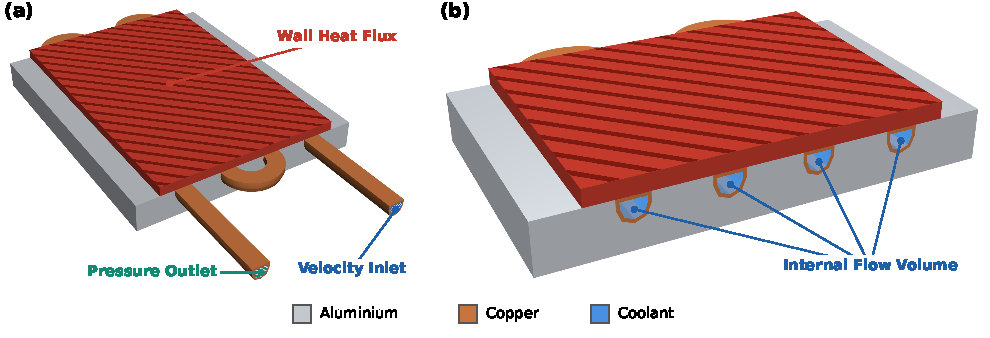
\includegraphics[width=\textwidth]{coldplate_figure.pdf}
    \caption{Cold-plate model used for the CHT analysis.
        (a)~Isometric view and (b)~cut showing the internal flow volume.}
    \label{fig:cfd_setup}
\end{figure}

The boundary conditions were chosen to match each test. The inlet was set as a
velocity inlet at the measured inlet temperature of the test (for example,
\SI{29.8}{\celsius} for the full-flow Galinstan test), with the velocity
adjusted to give the measured flow rate. The outlet was held at a pressure of
\SI{1}{atm}. The heat input was applied as a heat flux equal to the heat
reaching the cold plate, $\Qplate$, rather than the full electrical input,
because part of the input is lost to the environment
(\cref{sec:thermal-network}). For the full-flow Galinstan test this was about
\SI{60}{\watt} of the \SI{72}{\watt} input, and for the low-flow Galinstan test
about \SI{30}{\watt} of the \SI{40}{\watt} input, estimated from the measured
coolant temperature rise. The water run used the same $\Qplate$ as the water
tests, about \SI{62.6}{\watt}.

\begin{table}[htbp]
  \centering
  \caption{CHT simulation settings and boundary conditions.}
  \label{tab:simulation-setup}
  \small
  \begin{tabular}{@{}ll@{}}
    \toprule
    Parameter & Setting \\
    \midrule
    Analysis type    & Conjugate heat transfer \\
    Compressible     & Yes \\
    Flow model       & $k$--$\omega$ SST (turbulent); laminar for $\mathrm{Re} \leq 2110$ \\
    Time dependency  & Steady state \\
    Inlet            & Velocity inlet at the measured flow rate and inlet temperature \\
    Outlet           & Pressure outlet, \SI{1}{atm} \\
    Heat input       & Heat flux equal to $\Qplate$ of each test at the resistor footprints \\
    Mesh             & \num{427e3} cells (\cref{app:cht_validation}) \\
    \bottomrule
  \end{tabular}
\end{table}

Turbulent cases were solved with the $k$--$\omega$ SST turbulence model, and a
laminar model was used for the runs with an estimated $\mathrm{Re} \leq 2110$.
Mesh independence was therefore assessed separately for each flow regime and
each coolant. Each study was performed at the most demanding operating point,
the highest flow rate, where the boundary layers are thinnest, so that the
resulting mesh is conservative for all milder cases. Separate studies were
needed for the two coolants because Galinstan develops a thermal boundary layer
much thicker than its velocity boundary layer, whereas water has a thermal
boundary layer thinner than its velocity boundary layer and therefore requires
finer near-wall resolution for the temperature field. The same sequence of five
meshes, from \num{73e3} to \num{1.5e6} cells, was used in every study, and the
\num{427e3}-cell mesh was adopted. The mesh study, the iterative convergence and
the comparison with experiment are given in \cref{app:cht_validation}. In
addition to the runs that reproduce each test, the cold plate was simulated
with Galinstan at four flow rates between \SI{0.75}{\milli\litre\per\second}
and \SI{5}{\milli\litre\per\second}, to compare the simulated cold-plate
resistance with the $\varepsilon$--NTU model beyond the flows the rig could
reach (\cref{sec:rcp-calc}).

\subsection{Calculation of the Cold-Plate Resistance}
\label{sec:rcp-calc}

The cold-plate resistance $\Rcp$ cannot be measured directly, because the plate
temperature $T_\mathrm{P}$ is not measured. It is therefore inferred from the
resistor and inlet temperatures by removing the package resistance from the
total resistance of the network in \cref{eq:network}:
\begin{equation}
  \Rcp = \frac{\Tres - \Tin}{Q} - \Rpack,
  \label{eq:rcp-inferred}
\end{equation}
where $\Tres$ is the mean of the left and right resistor temperatures, $Q$ is
the heat passing into the coolant and $\Rpack = \SI{0.242}{\celsius\per\watt}$
is the package resistance calibrated on the turbulent water tests. The same
definition is applied to the experimental and simulated results, so that both
are compared with the model on an equal basis (\cref{fig:galinstan_rcp_cfd}).

\paragraph{Experimental values.} $Q$ is the heat reaching the plate,
$\Qplate$, obtained by subtracting the loss to ambient through $\Rmisc$ from the
electrical input, as in \cref{eq:network}. The flow rate is taken from a
combination of the EMF flow sensor and the energy balance,
$\Vdot = \Qplate / [\rho\cp(\Tout - \Tin)]$, which agreed closely for the tests
completed in this study.

\paragraph{Simulated values.} The conjugate heat transfer results are taken at
the final iteration of each run on the \num{427e3}-cell mesh. $Q$ is obtained
from the coolant energy balance at the simulated flow rate,
\begin{equation}
  Q = \rho\cp\Vdot\,(\Tout - \Tin),
\end{equation}
which gives \SIrange{57.4}{58.2}{\watt} for all four runs, and $\Tres$ is the
mean of the two resistor probe temperatures.

\paragraph{Model values.} The $\varepsilon$--NTU model gives
$\Rcp = 1/(\varepsilon\,\mdot\,\cp)$ with $\varepsilon = 1 - e^{-\NTU}$
(\cref{sec:eps-ntu}), using the Shah and London mean Nusselt number for laminar
flow (\cref{app:convection}). Because Galinstan has $\NTU > 10$ across this
range, the model is effectively the caloric limit, $\Rcp \approx 1/(\mdot\,\cp)$.
\edited{Changed from $\NTU > 30$: the model gives $\NTU \approx 35$ at
\SI{1.4}{\milli\litre\per\second} but about 10.7 at
\SI{5}{\milli\litre\per\second}, which is still caloric-limited.}

% ---------------------------------------------------------------------
\section{Experimental Procedure}
\label{sec:programme}

Two experiments were conducted to answer the two research questions.
Experiment~1 compares the thermal performance of the water and Galinstan loops
across a range of flow rates, and its data were used to build and validate the
thermal models of \cref{sec:thermal-model}. Experiment~2 demonstrates
Galinstan's ability to cool a power-dense inductor and quantifies the
additional eddy-current loss induced in the coolant by the inductor's magnetic
field. Temperatures throughout each loop were logged continuously for the
duration of every test.

\subsection{Experiment 1: Baseline Thermal Comparison}
\label{sec:exp1}

The first experiment establishes a baseline comparison of the two cooling loops
and was run on both using identical procedures. Before each test, the data
logger was started and the coolant was circulated at the target flow rate, set
by the pump current for Galinstan and by the pump duty cycle for water. The
resistors were then switched on at the test heat load. Each test continued
until the system reached steady state, taken as a change of less than
\SI{0.5}{\celsius} over 30 minutes. The thermocouple readings at the resistor,
the cold-plate inlet and the cold-plate outlet were then recorded, together with
the flow rate and the heat load. At shutdown, the resistors were switched off
before the pump was ramped down.

The planned tests are given in \cref{tab:flow-rates}. The full-flow tests
evaluate the maximum heat transfer of the current systems, and the low-flow
tests provide data to inform and validate the thermal models. The no-flow tests,
run at a reduced heat load of \SI{12}{\watt}, measure the heat leakage to the
environment and give $\Rmisc$ (\cref{sec:thermal-network}). Two further tests
at lower flow rates,
\SI{0.73}{\litre\per\minute} and \SI{0.5}{\litre\per\minute}, were later
conducted on the water loop, using the valve to reduce the flow below the
controllable range of the pump. These give laminar water data, in the same flow
regime as Galinstan. The low-flow Galinstan test was run at a reduced heat load
of \SI{40}{\watt}, so that the resistor and the pump housing stayed below the
\SI{70}{\celsius} limit set by the resin of the MHD pump~\cite{kwon_project_2025}.

\begin{table}[htbp]
  \centering
  \caption{Planned experimental flow rates.}
  \label{tab:flow-rates}
  \small
  \begin{tabularx}{\linewidth}{@{}lccL@{}}
    \toprule
    Test & Water & Galinstan & Goal \\
    \midrule
    Full flow & \SI{58.3}{\milli\litre\per\second} & \SI{1.4}{\milli\litre\per\second}
      & Evaluate the maximum heat transfer of the current systems \\
    Low flow  & \SI{29.2}{\milli\litre\per\second} & \SI{0.8}{\milli\litre\per\second}
      & Provide data to inform and validate the thermal models \\
    No flow   & \SI{0}{\milli\litre\per\second}    & \SI{0}{\milli\litre\per\second}
      & Assess heat leakage to the environment \\
    \bottomrule
  \end{tabularx}
\end{table}

\subsection{Experiment 2: Inductor Cooling and Eddy-Current Loss}
\label{sec:exp2}

The second experiment demonstrates the ability of Galinstan to cool a
power-dense inductor and assesses the interaction between its leakage field and
the electrically conductive coolant. The thermal test follows the procedure of
Experiment~1, except that the inductor replaces the resistors. The inductor was
driven at its rated current of \SI{12}{\ampere} rms by an inverter and the
resonant tuning network of \cref{sec:capacitor-tuning}, giving an estimated heat
load of \SI{42.76}{\watt} (\cref{sec:model-validation}). The Galinstan was
operated at full flow, and the inductor temperatures were recorded with the
thermal camera. Any change in flow when the inductor was energised was captured
by the flow sensor.

The eddy-current loss induced by the leakage field was measured separately with
an Agilent E4980A LCR meter at an excitation current of about \SI{5}{\milli\ampere},
by recording the AC resistance $R_{\mathrm{ac}}$ of the inductor winding in four
configurations: (i)~the inductor alone, (ii)~the inductor on the
empty cold plate, (iii)~the inductor on the cold plate filled with Galinstan, and
(iv)~the inductor on the cold plate with a PVC vial of Galinstan standing beside
it, as shown in \cref{fig:vial-setup}. Any conductor in the leakage field adds
to the series resistance seen at the winding, so the change in resistance
between two configurations isolates the loss of the conductor that was added.
The measurements were taken at the \SI{85}{\kilo\hertz} operating frequency.
Because Galinstan and the cold plate are linear and non-magnetic, the added loss
at any current is $\Delta R_{\mathrm{ac}} I_{\mathrm{rms}}^{2}$, so the change in
resistance is a direct measure of the eddy-current loss. Finally, with the cold
plate removed, the vial was moved progressively further away from the inductor,
from \SIrange{1}{5}{\centi\metre}, to show how the loss in the coolant falls
with distance.

\begin{figure}[htbp]
  \centering
  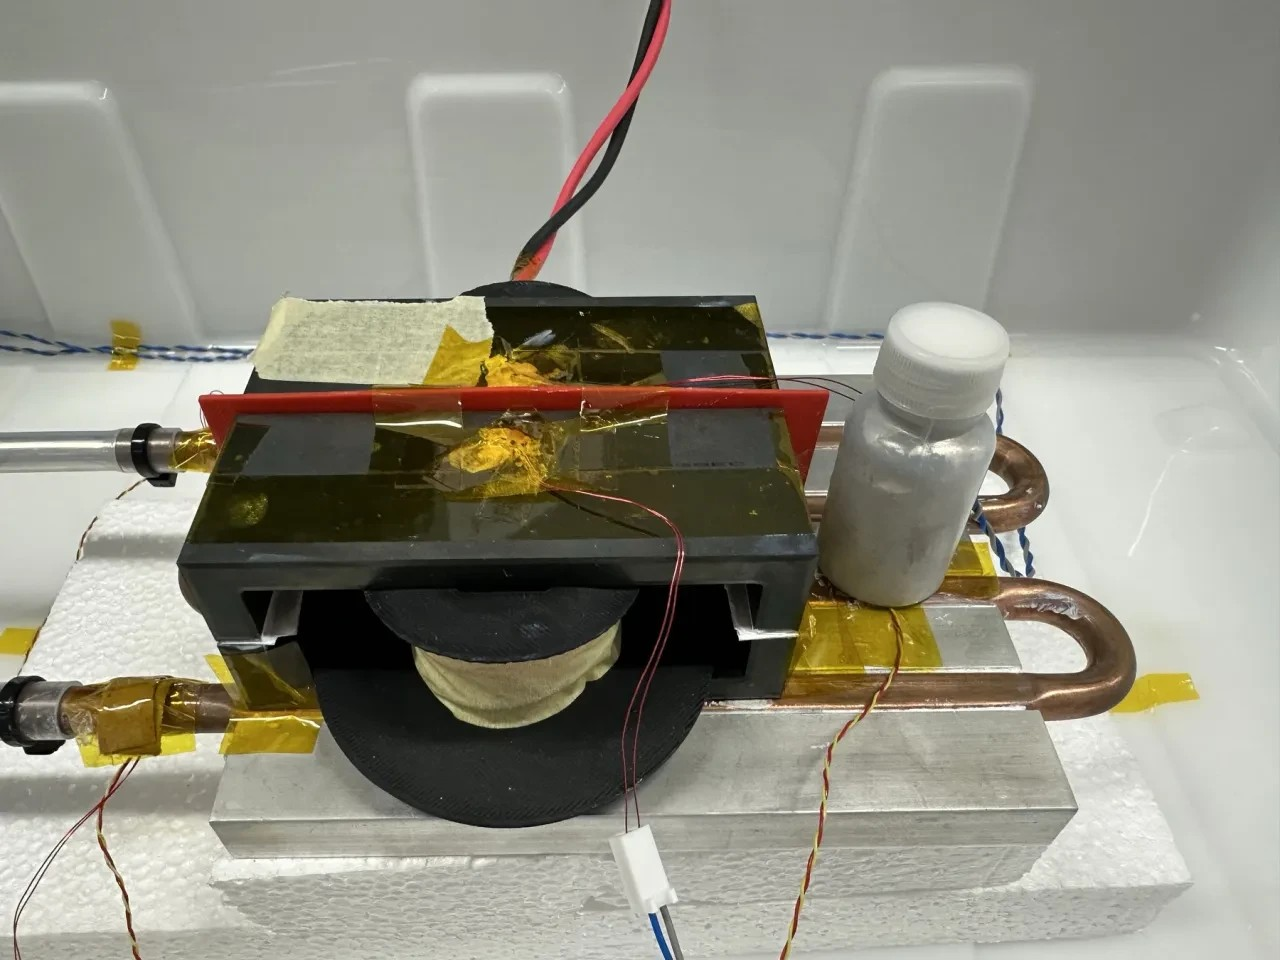
\includegraphics[width=0.6\linewidth]{inductor_vial_setup}
  \caption{Inductor on the Galinstan cold plate, with the PVC vial of Galinstan
    standing beside it, as used for configuration~(iv) of the eddy-current loss
    measurement.}
  \label{fig:vial-setup}
\end{figure}

% =====================================================================
%  Chapter 4 --   Results
% =====================================================================

\chapter{Results}
\label{ch:results}

\subsection{Analytical Thermal Models}

Table~\ref{tab:tn_results} compares the measured and predicted resistor
temperature $T_\mathrm{M}$ and coolant outlet temperature $T_\mathrm{out}$.
$R_\mathrm{pack}$ was calibrated on the two turbulent water tests, so those rows
check the method's consistency rather than validate it independently. Likewise,
Galinstan $T_\mathrm{out}$ is computed from the energy-balance flow rate and
agrees closely by construction. The independent test of the model is therefore
$T_\mathrm{M}$ in the Galinstan and laminar water tests.

\begin{table}[htbp]
    \centering
    \caption{Measured and predicted temperatures
        ($R_\mathrm{pack} = \SI{0.242}{\celsius\per\watt}$; turbulent water
        $R_\mathrm{cp}$ from the ATS datasheet, laminar water from the
        $\varepsilon$-NTU model). $\dagger$~Calibration tests. Galinstan
        $T_\mathrm{out}$ uses the energy-balance flow, so it agrees by construction.}
    \label{tab:tn_results}
    \begin{tabular}{lcccc}
        \toprule
        Test & \multicolumn{2}{c}{$T_\mathrm{M}$ (\si{\celsius})}
             & \multicolumn{2}{c}{$T_\mathrm{out}$ (\si{\celsius})} \\
        \cmidrule(lr){2-3}\cmidrule(lr){4-5}
             & Measured & Predicted & Measured & Predicted \\
        \midrule
        Galinstan \SI{1.4}{\milli\litre\per\second}               & 59.3 & 61.8 & 47.6 & 47.4 \\
        Galinstan \SI{0.75}{\milli\litre\per\second} (\SI{40}{\watt}) & 51.1 & 51.1 & 43.6 & 43.6 \\
        Water \SI{3.6}{\litre\per\minute}$^\dagger$               & 49.2 & 49.3 & 33.5 & 33.4 \\
        Water \SI{1.8}{\litre\per\minute}$^\dagger$               & 48.6 & 48.6 & 32.7 & 32.5 \\
        Water \SI{0.73}{\litre\per\minute}                        & 50.1 & 53.1 & 33.3 & 34.9 \\
        Water \SI{0.5}{\litre\per\minute}                         & 50.5 & 54.1 & 33.9 & 35.7 \\
        \bottomrule
    \end{tabular}
\end{table}

The predicted $T_\mathrm{M}$ lies within the $\pm\SI{3.1}{\celsius}$ measurement
band in five of the six tests, with an RMS error of \SI{1.8}{\celsius} for
Galinstan and \SI{2.3}{\celsius} for water. The turbulent water tests agree
within \SI{0.1}{\celsius}. The mid-flow Galinstan test
(\SI{1.0}{\milli\litre\per\second}) is excluded because its energy balance
closed at only about \SI{80}{\percent}, which indicates a flow-measurement error
or an incomplete approach to steady state.

The two laminar water tests are over-predicted by \SI{3.0}{\celsius} and
\SI{3.6}{\celsius}. In the laminar regime the model's $R_\mathrm{cp}$ rises to
\SIrange{0.074}{0.088}{\celsius\per\watt}, three to four times the turbulent
value. The measurements show no such loss: $T_\mathrm{M} - T_\mathrm{in}$ stays
between \SI{16.1}{\celsius} and \SI{16.6}{\celsius} from
\SIrange{3.6}{0.5}{\litre\per\minute}, and the measured $R_\mathrm{cp}$ follows
the manufacturer's turbulent trend (Figure~\ref{fig:flow_sweep}). This suggests
the flow in these tests was not fully laminar. The flow meter is uncertain below
\SI{1}{\litre\per\minute}, and the Reynolds number scales with
$\dot{V}/\mu$. With $\mu \approx \SI{0.75}{\milli\pascal\second}$ at the
\SI{33}{\celsius} test temperature, the \SI{0.73}{\litre\per\minute} test
reaches $\mathrm{Re} \approx 2600$, inside the transitional range, and any
under-reading of the flow would raise this further. Disturbances from the inlet
and U-bends can also persist at $\mathrm{Re} \approx$ 1300--1900, where the
development length of 66--97 tube diameters far exceeds the 19-diameter pass
length. If these tests are treated as turbulent, the datasheet trend predicts
$T_\mathrm{M}$ within \SI{0.7}{\celsius}. The laminar prediction is therefore
best read as a conservative upper bound. In the turbulent range the
$\varepsilon$-NTU model lies within \SI{15}{\percent} of the datasheet
(\SI{0.024}{\celsius\per\watt} against \SI{0.021}{\celsius\per\watt} at
\SI{2}{\litre\per\minute}).

Galinstan is caloric-limited at every tested flow: at least \SI{97}{\percent} of
its cold-plate resistance is $R_\mathrm{cal}$, so the pump, not the cold-plate
geometry, sets its thermal performance. Hodes et al.~\cite{hodes2014} reached
the same conclusion. Galinstan's volumetric heat capacity is 0.45 times that of
water, and caloric resistance made up \SI{55}{\percent} of the total for their
optimised Galinstan minichannel against \SI{40}{\percent} for water. The larger
share found here reflects a flow rate far below their optimum, and it means
higher pump flow, not improved convection, is the main route to better
liquid-metal performance in this system.
% =====================================================================
%  Chapter 5 -- Discussion
%  Structure follows Kwon (2025): interpretation of results, validity and
%  limitations, relevance to the field.
% =====================================================================
\chapter{Discussion}
\label{sec:discussion}

This chapter interprets the results of \cref{ch:results} against the two
research questions. The thermal performance and pumping power of the Galinstan
loop are discussed first (RQ1), followed by the inductor experiment (RQ2). The
validity and limitations of the measurements and models are then considered,
and finally the relevance of the findings to the cooling of PECs.

% ---------------------------------------------------------------------
\section{Interpretation of Results}
\label{sec:disc-interpretation}

\subsection{Thermal Performance of Galinstan in the Tested Cold Plate}
\label{sec:disc-performance}

The results in \cref{sec:results-measured} show that, at the flow rates
achieved, the Galinstan loop cooled the resistors less effectively than the
water loop, with a total thermal resistance 1.8 to 3.1 times higher
(\cref{tab:measured-performance}). However, the Galinstan tests ran at
\SIrange{0.8}{1.5}{\milli\litre\per\second}, one to two orders of magnitude below
the water tests (\SIrange{8.3}{58.3}{\milli\litre\per\second}). The comparison
therefore reflects the flow the MHD pump could deliver rather than a general
disadvantage of Galinstan as a coolant.

The reason lies in the limiting regime of the cold plate. Galinstan's NTU was 35
to 65 in the tests, so $\varepsilon \approx 1$ and $\Rcp \approx 1/(\mdot\,\cp)$.
The coolant therefore leaves the plate at almost the plate temperature, and heat
removal is limited by the ability of the flow to store and transport heat.
Galinstan's high thermal conductivity gives a wall heat transfer coefficient of
about \SI{7700}{\watt\per\metre\squared\per\kelvin}, roughly 7.5 times that of
laminar water (\cref{app:convection}). Its convective resistance $1/(hA)$ of
\SI{0.0085}{\celsius\per\watt} is lower than that of water even in turbulent
flow (\SIrange{0.012}{0.023}{\celsius\per\watt}). This advantage, however, is
not used in the current setup, because the convective term accounts for less
than \SI{3}{\percent} of Galinstan's $\Rcp$. Water, by contrast, has
$\NTU \approx 0.3$--0.4 at every tested flow, so convection makes up about
\SI{85}{\percent} of its $\Rcp$. These results support H1: Galinstan lowers the
convective resistance, but its low volumetric heat capacity and low flow rate
give a caloric resistance at least as large as the package resistance, so the
total resistance of the Galinstan loop is higher than that of the water loop.

\Cref{fig:disc-regimes}(a) extends this analysis over the full flow range.
Galinstan remains caloric-limited ($\NTU > 3$) over the whole laminar range and
up to about \SI{50}{\milli\litre\per\second}. Water, in contrast, stays close to
the convection-limited boundary above about \SI{10}{\milli\litre\per\second}.
For a caloric-limited coolant, the most important property is the volumetric
heat capacity $\rho\cp$, and here water has the advantage
(\cref{tab:disc-properties}): it absorbs about 1.8 times more heat per unit
volume per degree.

The same behaviour gives the Galinstan loop a much larger actuation range.
Because its cold plate is caloric-limited, its resistance follows the flow:
roughly halving the Galinstan flow, from 1.45 to
\SI{0.77}{\milli\litre\per\second}, raised the total resistance from 0.488 to
\SI{0.799}{\celsius\per\watt} (\cref{tab:measured-performance}). The
convection-limited water plate, in contrast, barely responded, with the total
resistance changing only from 0.257 to \SI{0.267}{\celsius\per\watt} over a
seven-fold change in flow. As discussed in \cref{sec:reliability}, the
flow rate of a single-phase loop is the control input used to suppress the
temperature swing of a component, part of the reliability requirement for PEC
thermal management (\cref{tab:cooling-strategies}). The pressure of an MHD pump
scales directly with its current (\cref{sec:em-pumping}), so the Galinstan loop
offers direct control over the component temperature through the pump current
across a wide range. In the tested water loop, changing the flow had almost no
effect on the resistor temperature. This range comes at the cost of a higher
resistance at the flows achieved here, but it is an advantage where the
temperature swing, rather than the peak temperature, limits component lifetime.

\begin{table}[htbp]
  \centering
  \caption{Coolant properties relevant to suitability. Thermal properties are
    those used in the model (\cref{tab:coolant-properties}).}
  \label{tab:disc-properties}
  \small
  \begin{tabularx}{\linewidth}{@{}lrrX@{}}
    \toprule
    Property & Galinstan & Water & Implication \\
    \midrule
    $\rho\cp$ (\si{\mega\joule\per\metre\cubed\per\kelvin})
      & 2.33 & 4.18 & Water carries 1.8$\times$ more heat per unit flow \\
    $k$ (\si{\watt\per\metre\per\kelvin}) & 16.5 & 0.60
      & Galinstan $h$ is about 27$\times$ higher at equal Nu \\
    $\mu$ (\si{\milli\pascal\second}) & 2.4 & 1.0
      & Laminar pressure drop 2.4$\times$ higher at equal flow \\
    $\rho$ (\si{\kilogram\per\metre\cubed}) & 6370 & 1000
      & 6.4$\times$ coolant mass for the same volume \\
    Pr & 0.053 & 6.97 & Heat diffuses far faster than momentum in Galinstan \\
    Electrical conductivity (\si{\siemens\per\metre})
      & $3.46 \times 10^{6}$~\cite{noauthor_gainsn_nodate} & $\ll 1$
      & Galinstan can be pumped electromagnetically, but heats and is retarded
        in AC fields \\
    Liquid range at \SI{1}{atm} (\si{\celsius})
      & 10 to $>1300$~\cite{noauthor_gainsn_nodate,hodes_potential_2014}
      & 0 to 100 & Galinstan cannot boil at component temperatures \\
    \bottomrule
  \end{tabularx}
\end{table}
\edited{\Cref{tab:disc-properties}: citations added for the electrical
conductivity and liquid range, matching \cref{tab:galinstan-properties}. The
lower end of the liquid range was $-19$; it is now \SI{10}{\celsius}, the
melting point of the grade used in this work (\cref{tab:galinstan-properties}).}

\begin{figure}[htbp]
  \centering
  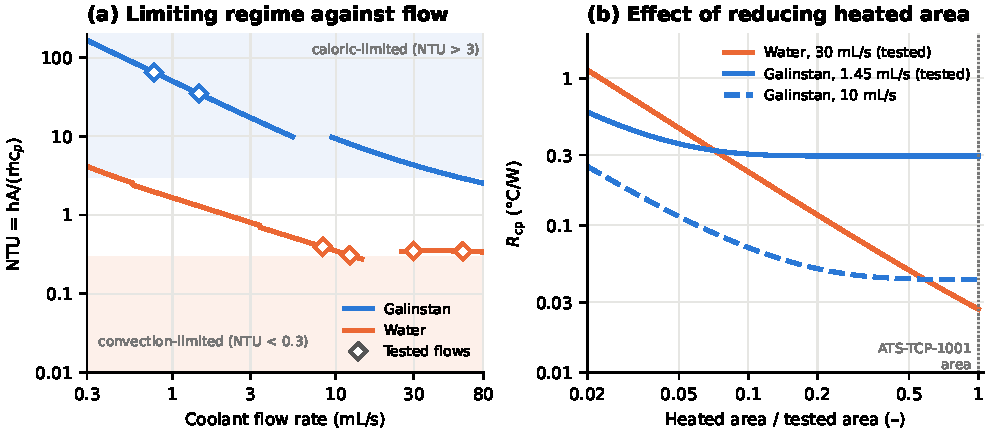
\includegraphics[width=\textwidth]{discussion_regimes.pdf}
  \caption{(a) NTU against flow rate for both coolants in the ATS-TCP-1001 cold
    plate, with the tested flows marked. Galinstan remains caloric-limited over
    the laminar range; water sits near the convection-limited boundary. Gaps
    mark the transitional range ($2300 < \mathrm{Re} < 4000$); turbulent
    Galinstan uses the Seban--Shimazaki correlation~\cite{bergman_fundamentals_2017}.
    (b) Indicative effect of reducing the heated area at fixed flow, with $h$
    held at its tested-geometry value. Water's $\Rcp$ rises in proportion to
    $1/A$, while Galinstan's at the tested flow is almost unaffected until the
    area falls to about a tenth of the tested value.}
  \label{fig:disc-regimes}
\end{figure}

\subsection{Pumping Power and Scalability}
\label{sec:disc-pumping}

RQ1 also asks how the pumping power of the two loops compares. At full flow, the
MHD pump drew \SI{0.85}{\watt}, about \SI{7}{\percent} of the \SI{11.5}{\watt}
drawn by the water pump, and it was more than 50 times smaller
(\cref{tab:pumps}). This is in line with An \emph{et al.}, who found that a
conduction pump drew less than \SI{15}{\percent} of the power of a mechanical
water pump for the same cooling performance~\cite{an_liquid_2024}, although here
the Galinstan loop also cooled less effectively. Per watt of pump power, the
Galinstan loop handled more heat, with a maximum coefficient of performance
(COP) of 200 against 47.6 for water. The low power draw does not, however,
reflect an efficient pump. The maximum mechanical efficiency of the MHD pump,
\SI{0.56}{\percent},
is an order of magnitude below the \SIrange{6}{10}{\percent} reported for DC
conduction pumps~\cite{an_liquid_2024,hodes_potential_2014}
(\cref{sec:em-pumping}), and far below the \SI{28.7}{\percent} of the
centrifugal water pump. Almost all of its input power is therefore dissipated
rather than delivered to the flow, which leaves considerable scope for a
redesigned pump. Fan \emph{et al.} show what is achievable: by reducing the
pressure drop of their loops to about one sixth with optimised connections and
cold plates, their MHD pumps reached flows of up to about
\SI{10}{\milli\litre\per\second} for less than
\SI{0.1}{\watt}~\cite{fan_liquid_2021,fan_high_2023} (\cref{tab:fan-comparison}). It is worth noting that the MHD pump was already at the
\SI{18}{\ampere} limit of its supply at full flow, so the Galinstan loop could
not be run at a higher flow.

For scalability, the more important question is the flow Galinstan would need
to match water. Because the cold plate is caloric-limited, the Galinstan $\Rcp$
is almost inversely proportional to the flow rate, as the simulations confirm up
to \SI{5}{\milli\litre\per\second} (\cref{fig:galinstan_rcp_cfd}). To match the
heat-capacity rate of
water at \SI{29.2}{\milli\litre\per\second} (\SI{122.0}{\watt\per\kelvin}),
Galinstan would need about \SI{52}{\milli\litre\per\second}, around 36 times the
full flow achieved here. The pressure of a DC conduction pump scales with current,
as shown by \cref{eq:mhd-pressure}, and the existing pump delivered
\SI{1.4}{\milli\litre\per\second} at the \SI{18}{\ampere} limit of its supply.
An increase in flow of this size would therefore require a redesigned pump
rather than simply a higher current. At equal volumetric flow, Galinstan also
needs about 2.4 times the pressure of water in laminar flow because of its higher
viscosity, and its density is 6.4 times that of water, which adds weight to the
loop (\cref{tab:disc-properties}). A comparison at equal pumping power, rather
than at the flow each pump could deliver, would therefore penalise Galinstan
further.

\subsection{Inductor Cooling and Eddy-Current Loss}
\label{sec:disc-inductor}

RQ2 asks whether the Galinstan loop can cool a power-dense inductor while adding
minimal loss, and how large the eddy-current loss induced in the coolant is. The
inductor was operated at an estimated loss of \SI{42.76}{\watt}, more than twice
the \SI{17.88}{\watt} datasheet loss limit above which its core requires active
cooling (\cref{sec:analytical-design}). Its maximum surface temperature was about
\SI{83}{\celsius} (\cref{fig:inductor-cam}), which shows that the Galinstan
loop can cool a power-dense inductor operating well beyond the loss its core
can dissipate without active cooling. The cooling effect of the plate is clear
from the steady-state thermal images: the upper core, which relies on natural
convection, ran markedly hotter than the lower core, which sits on the cold
plate (\cref{fig:inductor-cam-a}). This supports the first part of H2, that the
Galinstan loop cools the inductor beyond natural convection. The same difference
shows that the single-sided cold plate leaves part of the inductor's loss to be
removed by convection, and cooling both cores, as in the inductor of Gao
\emph{et al.}~\cite{gao_modeling_2022}, would make better use of the coolant.

The eddy-current measurements support the second part of H2. Placing the
inductor on the cold plate added \SI{11.7}{\milli\ohm} to the winding
resistance, whereas filling the plate with Galinstan added only
\SI{1.0}{\milli\ohm}, less than a tenth of the plate's own contribution. As
argued in H2,
the metal of the cold plate between the inductor and the
coolant is several skin depths thick at \SI{85}{\kilo\hertz}, so it shields the
Galinstan from the leakage field. Unshielded Galinstan is far more exposed: its
own skin depth at this frequency is about \SI{0.9}{\milli\metre} (for
$\sigma = \SI{3.46e6}{\siemens\per\metre}$~\cite{noauthor_gainsn_nodate}),
comparable to practical channel dimensions. The vial of Galinstan outside the
plate added \SI{10.3}{\milli\ohm}, an order of magnitude more than the coolant
inside the plate, although its volume and position differ. This agrees with the
initial ANSYS simulation, which found that \SI{1}{\milli\metre} of copper
shielding reduced the eddy-current loss in the coolant by more than
\SI{70}{\percent} (\cref{sec:inductor-design}). Without the plate, the effect of
the vial also fell with distance, from \SI{9.0}{\milli\ohm} at
\SI{1}{\centi\metre} to \SI{2.15}{\milli\ohm} beyond \SI{4}{\centi\metre}
(\cref{fig:rac_distance}), so keeping unshielded coolant a few centimetres from
the magnetics also limits the loss. Finally, the coolant flow did not change
measurably when the inductor was energised, which supports the final part of
H2.

% ---------------------------------------------------------------------
\section{Validity and Limitations}
\label{sec:disc-validity}

The steady-state data collected in this study are consistent across the two
loops and with the thermal models, but the conclusions rest on two Galinstan
tests and four water tests, and their limitations should be weighed. Four points
stand out.

First, the low-flow water results are limited by the flow measurement rather
than by the model. The measured $\Tres - \Tin$ stays between
\SI{16.1}{\celsius} and \SI{16.6}{\celsius} from
\SIrange{58.3}{8.3}{\milli\litre\per\second}, and the measured $\Rcp$ of
\SI{0.025}{\celsius\per\watt} at \SI{0.5}{\litre\per\minute} lies below water's
caloric limit $1/(\mdot\,\cp)$ of \SI{0.029}{\celsius\per\watt} at the indicated
flow (\cref{fig:water_rcp}). A cold plate cannot have $\Rcp < 1/(\mdot\,\cp)$, so
the true flow in that test must have been at least
\SI{9.6}{\milli\litre\per\second}, about \SI{15}{\percent} above the reading.
This supports the conclusion that the flow meter under-reads below its rated
range. It is also likely that these tests were not truly laminar. With the water
viscosity of about \SI{0.75}{\milli\pascal\second} at the \SI{33}{\celsius} test
temperature, the \SI{0.73}{\litre\per\minute} test reaches
$\mathrm{Re} \approx 2600$, in the transitional range, and any under-reading of
the flow raises this further. Disturbances from the pump, the valve and the
U-bends can also persist in the short passes, where the thermal entry length far
exceeds the pass length. If these tests are treated as turbulent, the datasheet
trend predicts $\Tres$ within \SI{0.7}{\celsius}, so the laminar
predictions in \cref{tab:tn_results} are best read as a conservative upper
bound.

Second, $\Rpack$ was calibrated on the turbulent water tests, where the plate is
close to isothermal. Galinstan's coolant temperature rise of
\SIrange{17}{18}{\celsius} violates this assumption: the outlet end of the plate
runs hotter than the mean, and the $\Rpack$ inferred for Galinstan ranges from
\SIrange{0.19}{0.24}{\celsius\per\watt} for an isothermal plate to
\SIrange{0.33}{0.51}{\celsius\per\watt} for uniform heat flux. The full-flow
Galinstan point lying slightly below its caloric limit (\cref{fig:galinstan_rcp})
is consistent with this. The Galinstan flow itself also relies on a small EMF,
which is less accurate at lower pump current, although it agreed with the energy
balance to within \SI{4}{\percent}. The lumped model therefore describes
Galinstan less reliably than water, although its prediction of the Galinstan
resistor temperatures to within \SI{2.5}{\celsius} (\cref{sec:results-tn})
shows that it captures the dominant behaviour.

Third, the conjugate heat transfer simulations address the main weakness of the
lumped model. They are mesh-independent above \num{427e3} cells and reproduce
all four probe temperatures within \SI{1.4}{\celsius} for both Galinstan tests.
The consistent over-prediction of the right-hand resistor by about
\SI{1.3}{\celsius} in both runs suggests a small systematic asymmetry in the
model, such as the heat-load distribution, rather than random error. For water,
the model under-predicts the resistor temperatures by about
\SIrange{2.3}{2.4}{\celsius}, which points to an over-predicted wall heat
transfer coefficient in the turbulent model (\cref{app:cht_validation}). The
model is therefore slightly pessimistic for Galinstan and optimistic for water,
so any advantage it shows for Galinstan is, if anything, understated. With this
in mind, the CHT model can be used with reasonable confidence to compare
geometries and flows that the test rig could not reach.

Fourth, the inductor experiment was run at a single operating point. Its heat
load is an estimate from the core-loss model and the measured winding
resistance, and the measured surface temperature of about \SI{83}{\celsius} is
above the \SI{65}{\celsius} assumed when the core loss was modelled, so the true
core loss will differ from the \SI{30.81}{\watt} estimate. The AC resistances
in \cref{fig:rac_configurations,fig:rac_distance} were measured at the
\SI{85}{\kilo\hertz} operating frequency, but each value comes from a single
measurement at low excitation, and the absolute resistance varied between
sessions, so only changes within a session are compared.

More generally, the study used a single cold plate designed for water, and the
coolants were compared at the flow each pump could deliver rather than at equal
pumping power. The water temperature rise across the plate was also below the
thermocouple accuracy, so the water energy balance could not be checked
independently.

% ---------------------------------------------------------------------
\section{Relevance to the Field}
\label{sec:disc-suitability}

The NTU analysis gives a clear criterion for where Galinstan is advantageous:
where the cooling surface, rather than the coolant flow, limits heat removal,
that is, where water would be convection-limited. \Cref{fig:disc-regimes}(b)
illustrates this using the $\varepsilon$--NTU model. The heated area is scaled
by a factor $f$ while the flow rate and heat transfer coefficient are held at
their values in the tested cold plate, so that $\NTU$ falls in proportion to $f$
and $\Rcp = 1/[\mdot\,\cp\,(1 - e^{-f\,\NTU_0})]$, where $\NTU_0$ is the value
for the full plate. This represents concentrating the same heat into a smaller
footprint or a shorter heated length, and the method and its assumptions are
given in \cref{app:area-scaling}. Reducing the heated area at fixed flow raises
water's $\Rcp$ almost in proportion, because water is already close to
convection-limited. At the tested flow, Galinstan's $\Rcp$ barely changes until
the area is reduced to about a tenth, because it simply uses up its excess
$hA$. At \SI{5}{\percent} of the tested area, Galinstan at
\SI{10}{\milli\litre\per\second} ($\Rcp \approx \SI{0.12}{\celsius\per\watt}$)
outperforms water at three times the flow
($\Rcp \approx \SI{0.46}{\celsius\per\watt}$). Galinstan's resistance only
begins to rise once $f\,\NTU_0$ falls to about 3, so a coolant that starts with a
large NTU can absorb a large reduction in area before its performance suffers.
Because $h$ is held fixed and pressure drop is not considered, the result is
indicative only, but it shows the type of application in which Galinstan's
conductivity becomes useful.
\edited{``About a fifth'' changed to ``about a tenth'': with $\NTU_0 = 34.9$ the
resistance starts to rise at $f \approx 3/\NTU_0 = 0.09$ (\cref{app:area-scaling}),
and \cref{tab:app-area} shows no change at $f = 0.2$. The caption of
\cref{fig:disc-regimes} was changed to match.}

Galinstan is therefore best suited to applications that combine (i)~high heat
flux over a small area, such as direct cooling of power semiconductors or local
hot spots, or minichannel and microchannel heat sinks; (ii)~a pump able to
deliver flow rates comparable to water, for which a sealed electromagnetic pump
with no moving parts may offer a reliability advantage; (iii)~component
temperatures near or above \SI{100}{\celsius}, where water would boil without
pressurisation; and (iv)~locations away from strong alternating magnetic fields,
or where the coolant is shielded from them by the cold plate, as in
\cref{sec:disc-inductor}.

In an IPT system, these criteria point to the power electronics, rather than the
pads, as the best place for Galinstan. In the \SI{10}{\kilo\watt} system of Kim
\emph{et al.}, the inverter and rectifier each dissipated about
\SIrange{70}{80}{\watt} in small switching devices placed away from the coupler,
where the heat flux is high and the magnetic field is weak
(\cref{sec:ipt-losses})~\cite{kim_thermal_2022}. The larger pad losses, by
contrast, are spread over about \SI{0.5}{\metre\squared} inside the strongest
alternating field at \SI{85}{\kilo\hertz}, so a cold plate under the pad would
see a low heat flux, for which water is adequate, together with a strong leakage
field. The inductor experiment shows that the leakage field need not rule
Galinstan out: coolant shielded by the metal of the cold plate added only
\SI{1.0}{\milli\ohm} to the winding resistance at \SI{85}{\kilo\hertz}, against
\SI{10.3}{\milli\ohm} for unshielded coolant beside the inductor
(\cref{sec:results-eddy}). Galinstan could therefore also cool compact
magnetics, such as the tank inductors and transformer, where heat is
concentrated in a small volume, provided the coolant is shielded.
\Cref{tab:disc-suitability} applies these criteria to the main components of an
IPT system.

\begin{table}[htbp]
  \centering
  \caption{Indicative suitability of Galinstan cooling for IPT system
    components, based on the criteria of \cref{sec:disc-suitability}.}
  \label{tab:disc-suitability}
  \small
  \begin{tabularx}{\linewidth}{@{}l>{\raggedright\arraybackslash}p{2.6cm}cX@{}}
    \toprule
    Component & Heat load character & Suitability & Reason \\
    \midrule
    Inverter and rectifier modules & High flux, small area & Good
      & Water likely convection-limited; much weaker AC fields than at the
        coupler \\
    Compact magnetics (tank inductors, transformer) & High flux, small volume
      & Possible
      & Leakage-field loss is small if the coolant is shielded by the cold
        plate (\cref{sec:results-eddy}) \\
    Coupler coils (Litz) and ferrite pads & Distributed, low flux & Limited
      & Large area, where water is adequate; strongest AC field, so the coolant
        must be shielded \\
    Resonant compensation capacitors & Moderate flux & Limited
      & Benefit only if close to their temperature limit; proximity to high
        voltage and AC fields \\
    Vehicle-side assembly & Weight-sensitive & Poor
      & 6.4$\times$ the coolant mass of water, and high material cost \\
    Large cold plates at low flow (as tested) & Low flux, large area & Poor
      & Caloric-limited; water carries 1.8$\times$ more heat per unit flow \\
    \bottomrule
  \end{tabularx}
\end{table}
\edited{\Cref{tab:disc-suitability}: coupler coils and pads changed from
``Poor'' to ``Limited'', since the eddy-current results show that a shielding
cold plate keeps the coolant's loss small, and a row added for compact magnetics,
which the inductor experiment represents.}

These findings agree with Hodes \emph{et al.}~\cite{hodes_potential_2014}, who
found that Galinstan's low volumetric heat capacity makes its caloric resistance
a larger share of the total than for water (\SI{55}{\percent} against
\SI{40}{\percent} in their optimised minichannel), and that its advantage depends
on geometries that exploit its high conductivity. The larger caloric share found
here (above \SI{97}{\percent}) reflects a cold plate designed for water and a
flow rate far below their optimum, rather than a contradiction of their result.
\issue{Check the volumetric heat-capacity ratio: Hodes quote 0.45, while the
properties used here give $2.33/4.18 = 0.56$; the difference is likely the
Galinstan $\cp$ (see the 360 vs \SI{366}{\joule\per\kilogram\per\kelvin} note).
\Cref{tab:galinstan-properties} also quotes 0.45.}

Despite the limitations above, the results show that a magnetohydrodynamically
pumped Galinstan loop can cool both a resistive load and a power-dense inductor,
and that the loss it adds near magnetics can be kept small when the coolant is
shielded by the cold plate. Its performance in the tested system is set by the
pump rather than by the coolant, so the case for liquid metal cooling in PECs
rests on higher-flow pumps and on cold plates designed to exploit its high
conductivity.

% ---------------------------------------------------------------------
\section{Recommendations for Further Work}
\label{sec:disc-limitations}

Further work should:
\begin{enumerate}
  \item compare the coolants at equal pumping power, using the CHT model to
    obtain the pressure drop as well as the temperature;
  \item test Galinstan at higher flow rates, closer to
    \SIrange{10}{30}{\milli\litre\per\second}, with an independently calibrated
    flow meter, which will require a redesigned pump;
  \item use the CHT model to evaluate small-area, high-flux geometries such as
    minichannel cold plates, where \cref{fig:disc-regimes}(b) indicates that
    Galinstan may outperform water;
  \item repeat the inductor test with the pump off and with the coolant
    unshielded, repeat the $R_{\mathrm{ac}}$ measurements to estimate their
    spread, and quantify eddy-current heating and MHD drag through coupled
    electromagnetic--thermal analysis before Galinstan is placed near an IPT
    coupler; and
  \item assess long-term material compatibility, since gallium alloys attack
    aluminium and copper requires protection at higher
    temperatures~\cite{an_liquid_2024}.
\end{enumerate}

% =====================================================================
%  Chapter 6 -- Conclusion
% =====================================================================
\chapter{Conclusion}
\label{ch:conclusion}

As PECs become more power-dense, removing their losses from a smaller volume
increasingly limits their design. This project evaluated MHD-pumped Galinstan as
a coolant for such converters, and identified where in an IPT system it is most
useful. A Galinstan loop and a water loop were compared on the same commercial
cold plate under resistive heat loads, the results were interpreted with an
$\varepsilon$--NTU thermal network and extended with a validated conjugate heat
transfer simulation, and the Galinstan loop was used to cool a power-dense
\SI{85}{\kilo\hertz} planar inductor.

\textbf{RQ1.} At the flows each pump could deliver, water outperformed
Galinstan, with a total resistance from the resistor to the coolant inlet of
\SIrange{0.257}{0.267}{\celsius\per\watt} against
\SIrange{0.488}{0.799}{\celsius\per\watt}. The $\varepsilon$--NTU analysis
explains this result and supports H1. Galinstan's high thermal conductivity
reduced its convective resistance to less than \SI{3}{\percent} of the cold-plate
resistance, but at \SIrange{0.77}{1.45}{\milli\litre\per\second} the plate was
caloric-limited, so Galinstan's low volumetric heat capacity set its
performance. The water plate, in contrast, was convection-limited and barely
responded to a seven-fold change in flow. The MHD pump drew only
\SI{0.85}{\watt}, against \SI{11.5}{\watt} for the water pump, giving a maximum
COP of 200 against 47.6, but its mechanical efficiency was only
\SI{0.56}{\percent}. The simulation shows that at
\SI{5}{\milli\litre\per\second}, the limit of laminar flow, the Galinstan total
resistance would fall to about \SI{0.29}{\celsius\per\watt}, within
\SI{14}{\percent} of water at a lower flow than any of the water tests.

\textbf{RQ2.} The Galinstan loop cooled the inductor, running at more than twice
the loss its core can dissipate without active cooling, to a maximum surface
temperature of about \SI{83}{\celsius}. Galinstan inside the cold plate added
only \SI{1.0}{\milli\ohm} to the winding AC resistance at
\SI{85}{\kilo\hertz}, against \SI{11.7}{\milli\ohm} for the plate itself and
\SI{10.3}{\milli\ohm} for unshielded Galinstan beside the inductor. The metal of
the cold plate therefore shields the coolant from the leakage field, supporting
H2, although the effect of the field on the flow could not be confirmed.

The main contribution of this work is to show when Galinstan is worth using.
Its advantage lies not in its conductivity alone, but in applications where the
heated area is small and the heat flux high: at \SI{5}{\milli\litre\per\second},
the model predicts that it outperforms water once the heated area falls below
about \SI{40}{\centi\metre\squared}. In an IPT system, this points to the
inverter and rectifier modules and to shielded compact magnetics, rather than
the large, distributed losses of the pads. These conclusions rest on a small
number of tests on a single cold plate designed for water, and the area
analysis is indicative only. Realising Galinstan's advantage will require a more
efficient, higher-flow pump with integrated power electronics, and a smaller cold
plate designed for liquid metal (\cref{sec:disc-further-work}).


%\backmatter
%\printbibliography[heading=bibintoc,title={References}]

%\appendix
% cleveref does not detect \appendix here, so appendix chapters were cited as
% "Chapter A". Label them (and their sections) as appendices explicitly; the
% names are set with the other \crefname commands in the preamble.
%\crefalias{chapter}{appendix}
%\crefalias{section}{subappendix}
%% =====================================================================
% Appendix: Validation of the SimScale conjugate heat transfer model
% Requires: graphicx, subcaption, siunitx (v2 \SI syntax, as in main report)
% =====================================================================

\chapter{Conjugate Heat Transfer Model}
\label{app:cht_validation}

The SimScale conjugate heat transfer (CHT) model was checked in three stages
before its results were used: a mesh independence study to bound the
discretisation error, a check of iterative convergence, and a comparison of the
converged probe temperatures against the experimental measurements. The
acceptance criterion throughout was the $\pm\SI{2.2}{\celsius}$ tolerance of the
thermocouples. Numerical errors well inside this band can be neglected, so any
remaining disagreement with experiment can be attributed to the modelling
assumptions or to the measurements themselves.

\subsubsection{Flow Regime and Mesh Independence}

Turbulent cases were solved with the $k$--$\omega$ SST turbulence model, and a
laminar model was used for runs with an estimated $\mathrm{Re} \leq 2110$.
Because the two models resolve the near-wall region differently, mesh
independence was assessed separately for each flow regime and each coolant.
Each study was performed at the most demanding operating point in its regime,
the highest flow rate, where the boundary layers are thinnest and the near-wall
gradients steepest. A mesh that resolves this case is therefore conservative for
the lower flow rates in the same regime. Separate studies were needed for the
two coolants because their Prandtl numbers differ by more than two orders of
magnitude. Galinstan ($\mathrm{Pr} \sim 10^{-2}$) develops a thermal boundary
layer much thicker than its velocity boundary layer, whereas water
($\mathrm{Pr} \approx 5$--$7$) has a thermal boundary layer thinner than its
velocity boundary layer and so needs finer near-wall resolution to capture the
temperature field. The same sequence of five meshes, from \num{73e3} to
\num{1.5e6} cells, was used in every study.
% NOTE: your earlier paragraph said "three" meshes; the figure shows five.

Figure~\ref{fig:mesh_independence} shows the study for Galinstan at
\SI{1.4}{\milli\litre\per\second}. The inlet and outlet temperatures vary by
less than \SI{0.1}{\celsius} across the full range. The inlet is fixed by the
boundary condition and the outlet is set largely by the bulk energy balance, so
neither depends strongly on near-wall resolution. The resistor temperatures are
the sensitive quantities, because they depend on resolving conduction through
the cold plate and the temperature gradient at the wall. The two coarsest
meshes underpredict them by up to \SI{2.75}{\celsius} relative to the finest
mesh, which exceeds the thermocouple tolerance. From \num{427e3} cells upward,
every probe lies within \SI{0.25}{\celsius} of the \num{1.5e6}-cell result.
Convergence is not strictly monotonic: the \num{427e3}- and \num{655e3}-cell
meshes slightly overshoot the finest mesh, and the refinement ratio between
successive meshes is not constant. Richardson extrapolation and the grid
convergence index, which assume monotonic convergence at a fixed refinement
ratio, were therefore not applied. Instead, the \SI{0.25}{\celsius} residual
change was compared directly with the measurement tolerance, and it is about
one ninth of that tolerance. The \num{427e3}-cell mesh was adopted for the
Galinstan simulations because it is the coarsest mesh whose discretisation
error is negligible against the measurement uncertainty.
% CHECK: confirm 427k is the mesh actually used for the reported runs.

\begin{figure}[htbp]
    \centering
    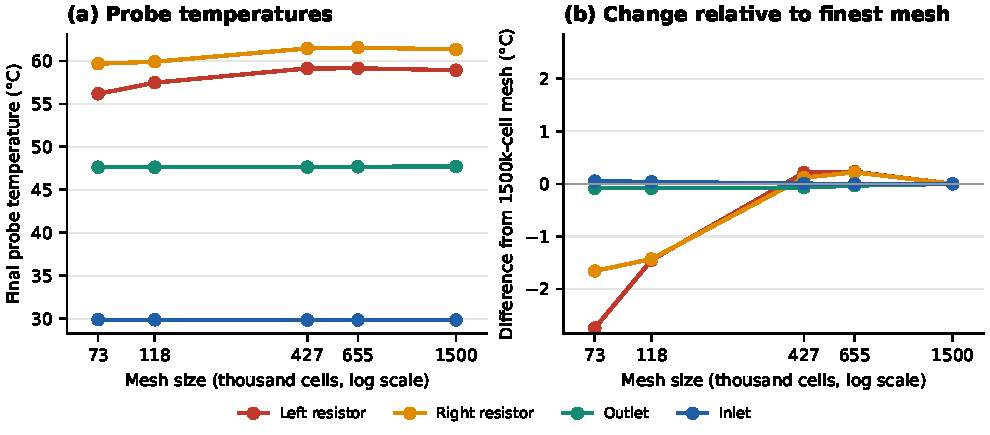
\includegraphics[width=\textwidth]{mesh_independence.pdf}
    \caption{Mesh independence study for Galinstan at
        \SI{1.4}{\milli\litre\per\second}: (a) final probe temperatures and
        (b) change relative to the \num{1.5e6}-cell mesh. All probes change by
        less than \SI{0.25}{\celsius} between \num{427e3} and
        \num{1.5e6} cells.}
    \label{fig:mesh_independence}
\end{figure}

Figure~\ref{fig:mesh_independence_water} shows the corresponding study for
the turbulent water model at \SI{3.6}{\litre\per\minute}. The pattern is the
same: the inlet and outlet vary by less than \SI{0.03}{\celsius}, and the
resistor temperatures are underpredicted on the coarsest meshes, by up to
\SI{2.5}{\celsius} at \num{73e3} cells. The fine meshes settle more slowly than
they do for Galinstan, however. At \num{427e3} cells the resistors still differ
from the \num{1.5e6}-cell result by up to \SI{0.58}{\celsius}, and at
\num{655e3} cells by \SI{0.38}{\celsius}, compared with less than
\SI{0.25}{\celsius} for Galinstan on the same meshes. This is the behaviour the
Prandtl number argument predicts: the thinner thermal boundary layer in water
needs finer near-wall resolution before the wall temperature gradient, and
hence the resistor temperature, stops changing. Above \num{427e3} cells the
resistor temperatures fall monotonically with refinement, so the
\num{1.5e6}-cell result is itself probably still a few tenths of a degree from a
fully mesh-independent value. The \num{427e3}-cell mesh was retained for water.
Its discretisation error of about \SI{0.6}{\celsius} is roughly a quarter of the
thermocouple tolerance: acceptable for comparison with experiment, but not
negligible in the way it is for Galinstan.
% CHECK: confirm which mesh the water runs used. If 655k, replace the last two
% sentences: error about 0.4 C, roughly a sixth of the tolerance.
% NOTE: this is the turbulent water study. If a laminar water study (low flow)
% was also run, it needs its own figure or a sentence here.

\begin{figure}[htbp]
    \centering
    \figureorplaceholder[width=\textwidth]{mesh_independence_water.pdf}
    \caption{Mesh independence study for water at
        \SI{3.6}{\litre\per\minute} ($k$--$\omega$ SST): (a) final probe
        temperatures and (b) change relative to the \num{1.5e6}-cell mesh,
        plotted on the same scale as Figure~\ref{fig:mesh_independence}. The
        inlet and outlet differ by only \SI{0.26}{\celsius} and overlap in (a).
        The resistor temperatures change by up to \SI{0.58}{\celsius} between
        \num{427e3} and \num{1.5e6} cells.}
    \label{fig:mesh_independence_water}
\end{figure}
\issue{The measured full water flow is now \SI{3.5}{\litre\per\minute}
(\SI{58.3}{\milli\litre\per\second}) in the main text. This appendix still says
the water simulations ran at \SI{3.6}{\litre\per\minute}. If that is the flow
set in SimScale, keep it and say so; otherwise change it to
\SI{3.5}{\litre\per\minute}.}

\subsubsection{Iterative Convergence}

The model was solved as a steady-state problem, and convergence was judged by
monitoring the probe temperatures, since these are the quantities compared
against experiment (Figure~\ref{fig:simscale_full}). The inlet temperature
settles within about 150 iterations because it is fixed by the boundary
condition. The outlet and resistor temperatures relax far more slowly, decaying
over several thousand iterations after an initial overshoot. This behaviour is
typical of conjugate heat transfer: heat crosses the solid regions by
conduction alone, so the solid temperature field relaxes much more slowly than
the flow field. By 4000 iterations the outlet temperature had levelled off,
while the resistor temperatures were still falling by about \SI{0.3}{\celsius}
over the final 1000 iterations.
% CHECK: drift read from the plot; confirm from the exported probe data.
The fully converged resistor temperatures would therefore be slightly lower
than those reported. This drift is small relative to the measurement tolerance,
but it is not zero, and its direction matters for the comparison below: it would
move the right resistor towards the measured value and the left resistor
slightly further below it. The water model converges much faster
(Figure~\ref{fig:simscale_water}). After an initial transient, every probe is
within \SI{0.01}{\celsius} of its final value by about 1000 iterations, and at
every mesh density no probe changes by more than \SI{0.001}{\celsius} over the
final 1000 iterations. Iterative error is therefore negligible for water.

\begin{figure}[htbp]
    \centering
    \begin{subfigure}{\textwidth}
        \centering
        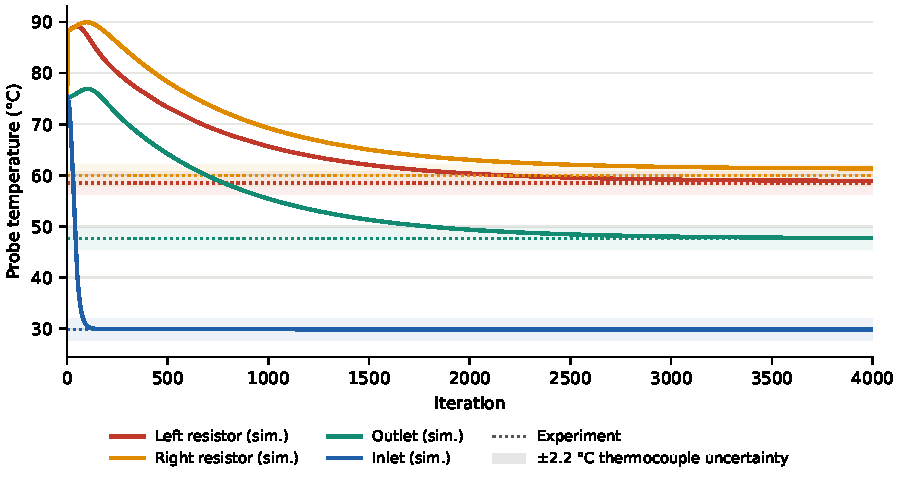
\includegraphics[width=0.9\textwidth]{simscale_convergence_full.pdf}
        \caption{Galinstan, \SI{1.4}{\milli\litre\per\second} (\SI{72}{\watt})}
        \label{fig:simscale_full}
    \end{subfigure}

    \vspace{0.6em}
    \begin{subfigure}{\textwidth}
        \centering
        \figureorplaceholder[width=0.9\textwidth]{simscale_convergence_water.pdf}
        \caption{Water, \SI{3.6}{\litre\per\minute} (\SI{72}{\watt}),
            \num{427e3} cells}
        \label{fig:simscale_water}
    \end{subfigure}
    \caption{Convergence of the SimScale conjugate heat transfer model against
        experiment. Solid lines show the simulated probe temperatures at each
        iteration; dotted lines show the measured values, with shaded bands for
        the $\pm\SI{2.2}{\celsius}$ thermocouple uncertainty. The measured
        resistor value is the mean of the two resistors. For Galinstan all
        probes lie within the measurement uncertainty at the final iteration;
        for water the resistors converge about \SI{2.4}{\celsius} below the
        measured value, just outside it.}
    \label{fig:simscale_convergence_both}
\end{figure}

\subsubsection{Comparison with Experiment}

For Galinstan, all four probes lie within the thermocouple tolerance of the
measured values at the final iteration (Figure~\ref{fig:simscale_full}). The inlet and outlet
agree to within about \SI{0.2}{\celsius}. The inlet agreement confirms that
the boundary condition was set correctly, rather than validating the model, and
the outlet agreement mainly confirms that the heat input and flow rate are
consistent with the energy balance. The resistor temperatures are the stronger
test, because they depend on the conduction path through the package and cold
plate and on the wall heat transfer coefficient the model predicts. The left
resistor is underpredicted by about \SI{0.5}{\celsius} and the right resistor
overpredicted by about \SI{1.4}{\celsius}. The model also predicts the right
resistor to be roughly \SI{2}{\celsius} warmer than the left, whereas the
measured temperatures are almost identical. This asymmetry lies within the
combined uncertainty, so the present instrumentation can neither confirm nor
rule it out.
\issue{The full-flow Galinstan data (\cref{fig:galinstan_transient}a) show the
right resistor at about \SI{60.1}{\celsius} and the left at about
\SI{58.6}{\celsius}, so the measured asymmetry is about \SI{1.5}{\celsius}, not
``almost identical''. The model's \SI{2}{\celsius} asymmetry is then close to
the measured one; reword this paragraph to match.}

The water model agrees less well (Figure~\ref{fig:simscale_water}). The
simulated inlet and outlet lie within \SI{0.15}{\celsius} of the measurements,
but this says little: the measured outlet rise is only \SI{0.4}{\celsius},
far below the sensor tolerance, so for water the outlet provides no useful
validation constraint. The resistors converge to \SI{46.9}{\celsius} and
\SI{46.8}{\celsius} against a measured mean of \SI{49.2}{\celsius}. They are
underpredicted by \SI{2.3}{\celsius} and \SI{2.4}{\celsius}, just outside the
tolerance band, and the resistor rise above the inlet is underpredicted by
about \SI{15}{\percent}. This gap is not a discretisation error. Refining the
mesh lowers the resistor temperatures further
(Figure~\ref{fig:mesh_independence_water}), so on the \num{1.5e6}-cell mesh the
underprediction grows to about \SI{2.9}{\celsius}. The discrepancy therefore
lies in the model itself. The cold plate, resistor package and their contact
are modelled identically for both coolants, and the Galinstan case shows no
comparable underprediction, which points towards the coolant side. The most
likely source is that the turbulent model overpredicts the wall heat transfer
coefficient for water. An error in the solid-side contact resistances that
happens to be masked in the Galinstan case cannot be excluded with only one
operating point per coolant.
% NOTE: measured values from Model Validation.xlsx ('FEM Model' sheet, water
% full flow): inlet 33.1, outlet 33.5, resistors 49.22 (mean). The raw log
% (CSV 17, 120-140 min) gives L 48.80, R 49.64 individually.

These results have clear limits. For Galinstan, agreement within
$\pm\SI{2.2}{\celsius}$ shows that the model is consistent with experiment at
the resolution of the measurements; it does not show that the model is
accurate to better than this. For water, the model is systematically optimistic,
predicting resistor temperatures about \SI{2}{\celsius} to \SI{3}{\celsius} too
low. The comparison also covers only one flow rate per coolant, so accuracy at
other operating points rests on the mesh study and the physical basis of the
model rather than on direct measurement. The model was therefore used where
these limits matter least: conclusions from the parametric studies are drawn
from trends and relative differences between configurations solved with the
same mesh and settings, which are less sensitive to systematic error than
absolute temperatures. The direction of the water bias also matters for the
coolant comparison. On average the model is slightly pessimistic for Galinstan and
optimistic for water, so any advantage the simulations show for Galinstan over
water is, if anything, understated.
% CHECK: confirm this matches how SimScale results are used in the main body.
%% =====================================================================
% Appendix: Convective heat transfer calculations for the thermal network
% Uses the report's macros: \Rcp, \Qplate, \Tin, \Tout, \mdot, \cp, \NTU, \Vdot
% Requires: amsmath, siunitx, booktabs, cleveref
% =====================================================================
\chapter{Convective Heat Transfer Calculations}
\label{app:convection}

This appendix explains how the cold-plate resistance $\Rcp$ in
\cref{sec:eps-ntu} is calculated from the flow rate and coolant properties, and
works through three of the tests in full.

\section{Heat Transfer Coefficient and Nusselt Number}

Heat passes from the tube wall into the coolant by convection, at a rate
\begin{equation}
  Q = hA\,(T_{\mathrm{wall}} - T_{\mathrm{f}}),
\end{equation}
where $A$ is the wetted area and $h$ the heat transfer coefficient
(\si{\watt\per\metre\squared\per\kelvin}). $h$ is not a material property; it
depends on the coolant, the flow and the geometry. Correlations therefore give
it in dimensionless form, as the Nusselt number
\begin{equation}
  \mathrm{Nu} = \frac{hD}{k}
  \qquad\Longrightarrow\qquad
  h = \frac{\mathrm{Nu}\,k}{D},
  \label{eq:app-nu}
\end{equation}
where $D$ is the tube bore and $k$ the coolant thermal conductivity. Nu is the
ratio of the heat actually removed by the flowing coolant to the heat that would
be conducted through a stationary layer of coolant of thickness $D$. Two
consequences matter here. First, for a given Nu, $h$ is proportional to $k$, so
Galinstan ($k = \SI{16.5}{\watt\per\metre\per\kelvin}$) gives roughly 27 times
the $h$ of water ($k = \SI{0.60}{\watt\per\metre\per\kelvin}$) at the same Nu.
Second, Nu depends on the flow regime and on how far along the tube the flow
has travelled, as described below.

\section{Flow Parameters}

Three dimensionless groups describe the flow:
\begin{align}
  \mathrm{Re} &= \frac{\rho u D}{\mu} = \frac{4\rho\Vdot}{\pi D \mu},
  & \mathrm{Pr} &= \frac{\mu\,\cp}{k},
  & \mathrm{Pe} &= \mathrm{Re}\,\mathrm{Pr},
  \label{eq:app-groups}
\end{align}
where $u$ is the mean velocity and $\Vdot$ the volumetric flow rate.
\begin{itemize}
  \item The \emph{Reynolds number} Re compares inertial and viscous forces. Below
    $\mathrm{Re} \approx 2300$ the flow is laminar, moving in smooth layers, and
    heat crosses the tube mainly by conduction. Above $\mathrm{Re} \approx 4000$
    it is turbulent, and eddies mix heat across the tube far more effectively. In
    between, the flow is transitional and unpredictable.
  \item The \emph{Prandtl number} Pr is a fluid property comparing how quickly
    momentum and heat diffuse. Water has $\mathrm{Pr} \approx 7$. Galinstan, like
    other liquid metals, has $\mathrm{Pr} \ll 1$ (0.053): its high conductivity
    spreads heat far faster than viscosity spreads momentum.
  \item The \emph{P\'eclet number} Pe compares heat carried along the tube by the
    flow with heat conducted across it. It controls how quickly the temperature
    profile develops.
\end{itemize}

\section{Thermal Entry Region}

Where the coolant first meets the heated wall, only a thin layer next to the
wall has warmed up. Heat has only a short distance to conduct across this thin
thermal boundary layer, so $h$ is high. Further along the tube the layer thickens
until it fills the bore; Nu then falls to a constant, \emph{fully developed}
value, which for laminar flow at constant wall temperature is
3.66~\cite{bergman_fundamentals_2017}. The length of this \emph{thermal entry
region} is measured by the dimensionless distance
\begin{equation}
  x^* = \frac{L}{D\,\mathrm{Re}\,\mathrm{Pr}} = \frac{L}{D\,\mathrm{Pe}},
  \label{eq:app-xstar}
\end{equation}
where $L$ is the heated length. Small values ($x^* < 0.01$) mean the flow
is still in the entry region over most of $L$; values above about 0.05 mean it is
fully developed over most of $L$. Equivalently, the thermal entry length is
approximately $L_{\mathrm{th}} \approx 0.05\,\mathrm{Re}\,\mathrm{Pr}\,D$.

The cold plate has four straight \SI{152}{\milli\metre} passes joined by
U-bends. The bends are assumed to mix the flow, so each pass is treated as a new
entry region with $L = \SI{152}{\milli\metre}$. Because every pass then has the
same mean Nu, this value applies to the whole heated area
$A = \pi D \times 4 \times \SI{0.152}{\metre} = \SI{0.0153}{\metre\squared}$.

\section{Correlations}

\paragraph{Laminar flow ($\mathrm{Re} < 2300$).} Shah and
London~\cite{shah_laminar_1978} give the mean Nusselt number over a heated
length $L$ of a circular tube at constant wall temperature, with a fully
developed velocity profile, as
\begin{equation}
\overline{\mathrm{Nu}}_T =
\begin{cases}
1.615\,(x^*)^{-1/3} - 0.7,  & x^* \le 0.005, \\[2pt]
1.615\,(x^*)^{-1/3} - 0.2,  & 0.005 < x^* < 0.03, \\[2pt]
3.657 + \dfrac{0.0499}{x^*}, & x^* \ge 0.03.
\end{cases}
\label{eq:app-shah}
\end{equation}
The first two branches describe the entry region, where Nu rises as
$(x^*)^{-1/3}$ as the boundary layer becomes thinner; the third tends to the
fully developed value of 3.657. This correlation was chosen because it gives the
mean Nu over the length, which is what $hA$ requires; it covers the entry
region, which is significant for short passes; and its constant wall
temperature matches the isothermal-plate assumption of \cref{sec:eps-ntu}.

\paragraph{Turbulent flow ($\mathrm{Re} \geq 4000$).} Gnielinski's
correlation~\cite{bergman_fundamentals_2017} is used for turbulent water:
\begin{equation}
  \mathrm{Nu} = \frac{(f/8)(\mathrm{Re} - 1000)\,\mathrm{Pr}}
                     {1 + 12.7\,(f/8)^{1/2}\left(\mathrm{Pr}^{2/3} - 1\right)},
  \qquad
  f = \left(0.790 \ln \mathrm{Re} - 1.64\right)^{-2},
  \label{eq:app-gnielinski}
\end{equation}
where $f$ is the Darcy friction factor for a smooth tube. It is valid from
$\mathrm{Re} \approx 3000$, lower than most turbulent correlations, which suits
the low end of the water flow range. Entry effects are neglected because
turbulent boundary layers develop within a few diameters.

\paragraph{Transitional flow ($2300 \le \mathrm{Re} < 4000$).} No correlation
is reliable here, so no value of $\Rcp$ is estimated in this range.

\paragraph{Turbulent liquid metal.} Gnielinski's correlation is not valid for
$\mathrm{Pr} < 0.5$. For turbulent Galinstan, which in this tube would require
more than about \SI{9.5}{\milli\litre\per\second}, the Seban--Shimazaki
correlation for a liquid metal at constant wall
temperature~\cite{bergman_fundamentals_2017} would apply instead:
\begin{equation}
  \mathrm{Nu} = 5.0 + 0.025\,\mathrm{Pe}^{0.8}.
  \label{eq:app-seban}
\end{equation}
No Galinstan test or simulation reached this regime.

\paragraph{Note on the plotted curves.} The three branches of
\cref{eq:app-shah} do not meet exactly: Nu jumps by about 0.5 at $x^* = 0.005$
and 0.3 at $x^* = 0.03$. In the flow-sweep figures these jumps are blended
smoothly over a factor of about 1.8 in $x^*$ either side of each join. Values
away from the joins, including every tested condition, are unchanged; the
largest change is about \SI{3}{\percent}, at the joins themselves.

\section{Calculation Procedure}

For each test, $\Rcp$ is calculated as follows.
\begin{enumerate}
  \item Calculate Re, Pr and Pe from the flow rate and properties using
    \cref{eq:app-groups}, and identify the regime.
  \item For laminar flow, calculate $x^*$ for one pass from \cref{eq:app-xstar} and
    $\overline{\mathrm{Nu}}$ from \cref{eq:app-shah}; for turbulent flow, use
    \cref{eq:app-gnielinski}.
  \item Convert to $h = \mathrm{Nu}\,k/D$ and multiply by $A$ to obtain the
    convective conductance $hA$.
  \item Calculate the heat-capacity rate $\mdot\,\cp = \rho\Vdot\cp$, then
    $\NTU = hA/(\mdot\,\cp)$ and $\varepsilon = 1 - e^{-\NTU}$.
  \item Obtain $\Rcp = 1/(\varepsilon\,\mdot\,\cp)$ and the coolant temperature
    rise $\Delta T_{\mathrm{cool}} = \Qplate/(\mdot\,\cp)$.
\end{enumerate}
For Galinstan, $\mdot\,\cp$ in step~4 is taken from the energy balance,
$\Qplate/(\Tout - \Tin)$, rather than the nominal EMF-sensor flow
(\cref{tab:tests}). Re and Nu are evaluated at the nominal flow; in fully
developed laminar flow Nu barely depends on flow, so this choice has no
practical effect.

\section{Worked Examples}

\paragraph{Example 1: water, \SI{12.2}{\milli\litre\per\second} (laminar, entry
region).}
\begin{align*}
  \Vdot &= \SI{12.2}{\milli\litre\per\second} = \SI{1.217e-5}{\metre\cubed\per\second}\\
  \mathrm{Re} &= \frac{4(1000)(1.217\times10^{-5})}{\pi(0.008)(0.001)} = 1936
    \quad\text{(laminar)}\\
  \mathrm{Pr} &= \frac{(0.001)(4182)}{0.60} = 6.97,
    \qquad \mathrm{Pe} = 1936 \times 6.97 = \num{13500}\\
  x^* &= \frac{0.152}{0.008 \times \num{13500}} = 0.00141
    \quad\text{(entry region, first branch)}\\
  \overline{\mathrm{Nu}} &= 1.615\,(0.00141)^{-1/3} - 0.7 = 13.7\\
  h &= \frac{13.7 \times 0.60}{0.008} = \SI{1028}{\watt\per\metre\squared\per\kelvin},
    \qquad hA = 1028 \times 0.0153 = \SI{15.7}{\watt\per\kelvin}\\
  \mdot\,\cp &= 1000\,(1.217\times10^{-5})\,(4182) = \SI{50.9}{\watt\per\kelvin}\\
  \NTU &= \frac{15.7}{50.9} = 0.31,
    \qquad \varepsilon = 1 - e^{-0.31} = 0.266\\
  \Rcp &= \frac{1}{0.266 \times 50.9} = \SI{0.074}{\celsius\per\watt}
\end{align*}
With $\Qplate = \SI{62.3}{\watt}$, $\Delta T_{\mathrm{cool}} =
62.3/50.9 = \SI{1.2}{\celsius}$. Since $x^* < 0.005$, the flow stays in the
entry region throughout each pass: the estimated thermal entry length,
$0.05\,\mathrm{Re}\,\mathrm{Pr}\,D \approx \SI{5.4}{\metre}$, is far longer than
the \SI{0.152}{\metre} pass. NTU is well below 1, so this test is
convection-limited: the convective term $1/(hA) = \SI{0.064}{\celsius\per\watt}$
makes up most of $\Rcp$.

\paragraph{Example 2: water, \SI{58.3}{\milli\litre\per\second} (turbulent).}
\begin{align*}
  \mathrm{Re} &= 9284 \quad\text{(turbulent)},
    \qquad \mathrm{Pr} = 6.97\\
  f &= (0.790\ln 9284 - 1.64)^{-2} = 0.0321\\
  \mathrm{Nu} &= \frac{(0.0321/8)(9284 - 1000)(6.97)}
                      {1 + 12.7\,(0.0321/8)^{1/2}\,(6.97^{2/3} - 1)} = 74.1\\
  h &= \frac{74.1 \times 0.60}{0.008} = \SI{5555}{\watt\per\metre\squared\per\kelvin},
    \qquad hA = \SI{85.0}{\watt\per\kelvin}\\
  \mdot\,\cp &= \SI{244.0}{\watt\per\kelvin}\\
  \NTU &= \frac{85.0}{244.0} = 0.35,
    \qquad \varepsilon = 1 - e^{-0.35} = 0.294\\
  \Rcp &= \frac{1}{0.294 \times 244.0} = \SI{0.0139}{\celsius\per\watt}
\end{align*}
Turbulence raises Nu about fivefold compared with Example~1, but the flow rate
is also five times higher, so NTU stays at about 0.35 and the cold plate remains
convection-limited. The model value is \SI{15}{\percent} below the datasheet
value of \SI{0.016}{\celsius\per\watt}, which is used for the temperature
predictions (\cref{sec:convection}).
\edited{Example~2 recalculated at the measured \SI{3.5}{\litre\per\minute}
(\SI{58.3}{\milli\litre\per\second}); it was \SI{3.6}{\litre\per\minute}.}

\paragraph{Example 3: Galinstan, \SI{1.4}{\milli\litre\per\second} (laminar,
fully developed).}
\begin{align*}
  \mathrm{Re} &= \frac{4(6370)(1.4\times10^{-6})}{\pi(0.008)(0.0024)} = 591
    \quad\text{(laminar)}\\
  \mathrm{Pr} &= \frac{(0.0024)(366)}{16.5} = 0.053,
    \qquad \mathrm{Pe} = 591 \times 0.053 = 31.5\\
  x^* &= \frac{0.152}{0.008 \times 31.5} = 0.603
    \quad\text{(fully developed, third branch)}\\
  \overline{\mathrm{Nu}} &= 3.657 + \frac{0.0499}{0.603} = 3.74\\
  h &= \frac{3.74 \times 16.5}{0.008} = \SI{7713}{\watt\per\metre\squared\per\kelvin},
    \qquad hA = \SI{117.9}{\watt\per\kelvin}\\
  \mdot\,\cp &= \frac{\Qplate}{\Tout - \Tin} = \frac{60.35}{17.83}
    = \SI{3.38}{\watt\per\kelvin}\\
  \NTU &= \frac{117.9}{3.38} = 34.8,
    \qquad \varepsilon = 1 - e^{-34.8} \approx 1.000\\
  \Rcp &= \frac{1}{1.000 \times 3.38} = \SI{0.295}{\celsius\per\watt}
\end{align*}
The temperature profile is fully developed within about \SI{13}{\milli\metre}
of each pass entry ($0.05\,\mathrm{Re}\,\mathrm{Pr}\,D$), so Nu is close to the
fully developed value. Despite the low Nu, Galinstan's high conductivity gives
an $h$ about 7.5 times that of Example~1. The cold plate is nevertheless
caloric-limited: the convective term $1/(hA) = \SI{0.0085}{\celsius\per\watt}$
is under \SI{3}{\percent} of $\Rcp$, and $\Rcp$ is essentially $1/(\mdot\,\cp)$.
Doubling $h$ would change $\Rcp$ by less than \SI{0.01}{\percent}; only a higher
flow rate reduces it.

\Cref{eq:app-shah} assumes the velocity profile is fully developed. For
Galinstan the hydrodynamic entry length ($0.05\,\mathrm{Re}\,D \approx
\SI{0.24}{\metre}$) exceeds the pass length, so the velocity and temperature
profiles develop together and the true Nu is somewhat higher. As shown above,
this has a negligible effect on $\Rcp$.

\begin{table}[htbp]
  \centering
  \caption{Summary of the worked examples.}
  \label{tab:app-examples}
  \small
  \setlength{\tabcolsep}{5pt}
  \begin{tabular}{@{}lccc@{}}
    \toprule
    & \multicolumn{2}{c}{Water} & Galinstan \\
    \cmidrule(lr){2-3}\cmidrule(l){4-4}
    & \SI{12.2}{\milli\litre\per\second} & \SI{58.3}{\milli\litre\per\second}
      & \SI{1.4}{\milli\litre\per\second} \\
    \midrule
    Re / regime & 1936 / laminar & 9284 / turbulent & 591 / laminar \\
    Pr & 6.97 & 6.97 & 0.053 \\
    $x^*$ & 0.0014 & -- & 0.60 \\
    Nu & 13.7 & 74.1 & 3.74 \\
    $h$ (\si{\watt\per\metre\squared\per\kelvin}) & 1028 & 5555 & 7713 \\
    $\mdot\,\cp$ (\si{\watt\per\kelvin}) & 50.9 & 244.0 & 3.38 \\
    NTU & 0.31 & 0.35 & 34.8 \\
    $\Rcp$ (\si{\celsius\per\watt}) & 0.074 & 0.0139 & 0.295 \\
    $1/(hA)$ share of $\Rcp$ & \SI{86}{\percent} & \SI{84}{\percent} & \SI{3}{\percent} \\
    Limiting regime & convection & convection & caloric \\
    \bottomrule
  \end{tabular}
\end{table}

\section{Effect of Heated Area}
\label{app:area-scaling}

\Cref{fig:area-scaling} estimates how $\Rcp$ would change if the same heat
were removed through a smaller heated area, for example a shorter heated length
or a smaller component footprint. It uses the $\varepsilon$--NTU relation of
\cref{sec:eps-ntu} with only the area changed.

\paragraph{Method.} The area is scaled by a factor $f$, $A \rightarrow fA$, while
the flow rate, coolant properties and heat transfer coefficient $h$ are held at
their values for the tested cold plate. The heat-capacity rate $\mdot\,\cp$ is
therefore unchanged, and the number of transfer units scales directly with $f$:
\begin{equation}
  \NTU(f) = f\,\NTU_0 = f\,\frac{hA_0}{\mdot\,\cp},
  \qquad
  \Rcp(f) = \frac{1}{\mdot\,\cp\left(1 - e^{-f\,\NTU_0}\right)},
  \label{eq:app-area}
\end{equation}
where $A_0 = \SI{0.0153}{\metre\squared}$ is the tested heated area and $hA_0$
is calculated as in \cref{eq:app-nu,eq:app-shah,eq:app-gnielinski}.
\Cref{tab:app-area} lists the inputs for the three cases plotted. Water at
\SI{30}{\milli\litre\per\second} represents the low-flow turbulent water test
(\SI{29.2}{\milli\litre\per\second}), and Galinstan at
\SI{1.5}{\milli\litre\per\second} the full-flow Galinstan test; using the exact
measured flows changes the resistances by less than \SI{4}{\percent} and does
not change the conclusions.

\begin{table}[htbp]
  \centering
  \caption{Inputs and results of the heated-area scaling.}
  \label{tab:app-area}
  \small
  \setlength{\tabcolsep}{5pt}
  \begin{tabular}{@{}lcccccc@{}}
    \toprule
    Case & $hA_0$ & $\mdot\,\cp$ & $\NTU_0$ & \multicolumn{3}{c}{$\Rcp$ (\si{\celsius\per\watt})} \\
    \cmidrule(l){5-7}
     & (\si{\watt\per\kelvin}) & (\si{\watt\per\kelvin}) & & $f = 1$ & $f = 0.2$ & $f = 0.05$ \\
    \midrule
    Water, \SI{30}{\milli\litre\per\second}      & 44.0  & 125.5 & 0.35 & 0.027 & 0.118 & 0.458 \\
    Galinstan, \SI{1.5}{\milli\litre\per\second}  & 118.1 & 3.50  & 33.8 & 0.286 & 0.286 & 0.351 \\
    Galinstan, \SI{5}{\milli\litre\per\second}    & 124.6 & 11.66 & 10.7 & 0.086 & 0.097 & 0.207 \\
    \bottomrule
  \end{tabular}
  \floatnote{Plotted in \cref{fig:area-scaling}.}
\end{table}


\paragraph{Interpretation.} The two coolants respond differently because they
start in different regimes.
\begin{itemize}
  \item Water starts with $\NTU_0 \approx 0.35$. For small NTU,
    $1 - e^{-\NTU} \approx \NTU$, so \cref{eq:app-area} reduces to
    $\Rcp \approx 1/(f\,hA_0)$: halving the area roughly doubles the resistance,
    which appears as a straight line on the logarithmic axes.
  \item Galinstan starts with $\NTU_0 \gg 1$, so $e^{-f\,\NTU_0}$ remains
    negligible and $\Rcp \approx 1/(\mdot\,\cp)$ until $f\,\NTU_0$ falls to about
    3. Its resistance therefore stays flat until
    \begin{equation}
      f \approx \frac{3}{\NTU_0} = \frac{3\,\mdot\,\cp}{hA_0},
    \end{equation}
    which is $f \approx 0.09$ at \SI{1.5}{\milli\litre\per\second} and
    $f \approx 0.28$ at \SI{5}{\milli\litre\per\second}. Below this point the
    excess convective capacity has been used up and $\Rcp$ begins to rise.
\end{itemize}
Galinstan's resistance falls below that of water at $f \approx 0.074$
(\SI{11}{\centi\metre\squared}) at \SI{1.5}{\milli\litre\per\second} and at
$f \approx 0.26$ (\SI{40}{\centi\metre\squared}) at
\SI{5}{\milli\litre\per\second}.
The comparison shows that a coolant with a large NTU can tolerate a large
reduction in heated area, and hence a large increase in heat flux, before its
cold-plate resistance increases, whereas a coolant near the convection-limited
boundary cannot.

\paragraph{Assumptions and limitations.}
\begin{itemize}
  \item $h$ is held at its value for the tested geometry. In a shorter laminar
    tube a larger fraction of the length would lie in the thermal entry region,
    raising the mean Nu; this would favour laminar water slightly at small $f$.
    In turbulent flow $h$ is nearly independent of length, so the effect is small
    for the cases shown.
  \item The plate is assumed to remain isothermal. With a smaller area the heat
    flux and the spreading resistance in the plate both increase, which this
    calculation does not capture.
  \item Pressure drop and pumping power are not considered; the flow rate is
    simply held constant.
  \item The coolant temperature rise $\Qplate/(\mdot\,\cp)$ is unchanged by $f$,
    so for Galinstan at low flow it remains \SIrange{17}{18}{\celsius}.
\end{itemize}
The results are therefore indicative of trends, not predictions for a specific
design. A minichannel or reduced-area design would need to be assessed with the
conjugate heat transfer model.
%% =====================================================================
% Appendix: FEMM current-flow model of the MHD pump (incomplete work)
% Source files: Part 4 Project/FEMM (MHD_pump.lua and report/)
% =====================================================================
\chapter{FEMM Model of the MHD Pump}
\label{app:femm}

A two-dimensional FEMM~4.2 current-flow model of the DC conduction pump was
started in this project to find how the drive current spreads through the
Galinstan channel, and from that the pumping force, the back-EMF and the pump
efficiency. The model was not completed or validated against measurements of
the pump, so it is not presented in the body of the report. This appendix
summarises the work to date as a starting point for the pump redesign
recommended in \cref{sec:disc-further-work}. All cases are generated by one
parametric Lua script, \texttt{MHD\_pump.lua}, held in the \texttt{FEMM} folder
of the project files.
\issue{Confirm that the modelled channel ($30 \times \SI{5}{\milli\metre}$),
\SI{20}{\milli\metre} electrodes and \SI{0.45}{\tesla} field match the built pump;
if not, describe the model as a representative geometry.}

\section{Model}

The model is drawn in the plane of the flow and the current, with the channel
depth as FEMM's out-of-plane depth (\cref{fig:femm-geometry}). The channel is
\SI{30}{\milli\metre} wide and \SI{5}{\milli\metre} deep, with copper electrodes
\SI{20}{\milli\metre} long, and extends \SI{120}{\milli\metre} beyond each
electrode so that the current fringing past the electrode ends is fully
captured. A current of \SI{18}{\ampere} is driven between the electrodes. FEMM's
current-flow solver has no magnetic field, so the force is found by integrating
$\mathbf{J} \times \mathbf{B}$ over a prescribed uniform field of
\SI{0.45}{\tesla}, and the flow is included by adding the motional EMF
$\mathbf{u} \times \mathbf{B}$ for plug flow of up to
\SI{5}{\milli\litre\per\second}. The resistance changed by less than
\SI{0.1}{\percent} when the mesh was refined twice.

\begin{figure}[htbp]
  \centering
  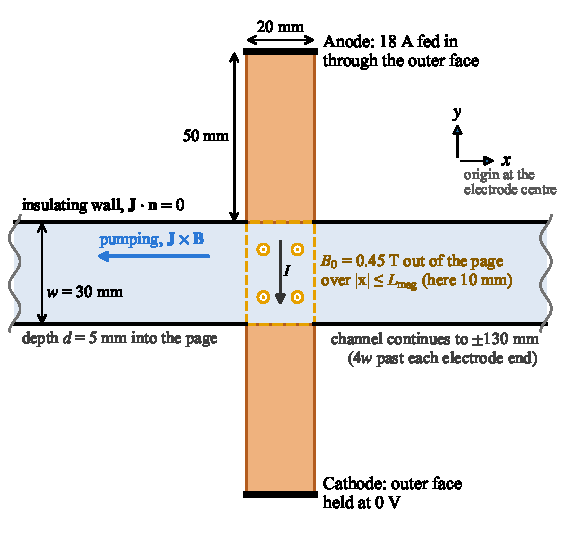
\includegraphics[width=0.6\linewidth]{femm_geometry}
  \caption{Geometry and boundary conditions of the FEMM pump model.}
  \label{fig:femm-geometry}
\end{figure}

\section{Results to Date}

At \SI{18}{\ampere}, the electrode-to-electrode resistance is
\SI{69.6}{\micro\ohm}, and about \SI{40}{\percent} of the current fringes past
the electrode ends, outside the field, where it produces no force
(\cref{fig:femm-jmap}). The model was reduced to a lumped circuit, in which the
Galinstan forms a parasitic path between the electrodes and a fringe path beyond
them, and this circuit reproduced the FEMM force and back-EMF to within
\SI{0.4}{\percent}. From it, the efficiency of the pump has a single peak
(\cref{fig:femm-efficiency}), whose height depends only on the electrode aspect
ratio and the series resistance. \Cref{tab:femm-results} summarises the main
design results.

\begin{figure}[htbp]
  \centering
  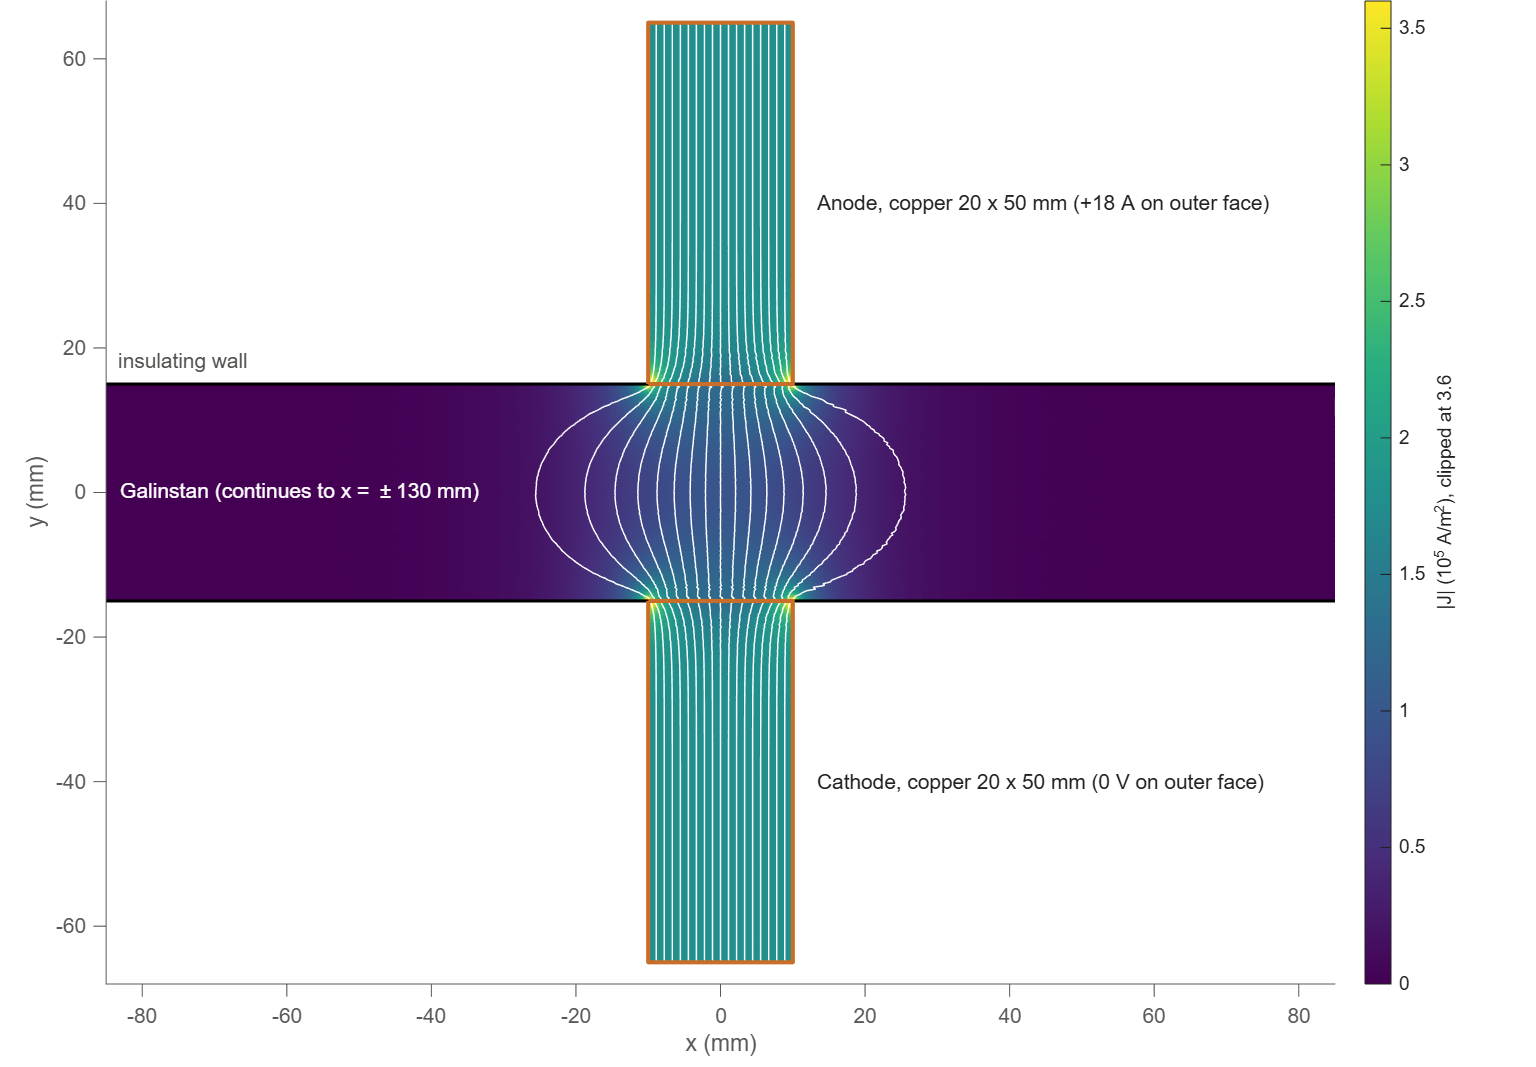
\includegraphics[width=0.6\linewidth]{femm_J_map}
  \caption{Current density in the pump channel at \SI{18}{\ampere}, no flow.}
  \label{fig:femm-jmap}
  \floatnote{Streamlines \SI{1}{\ampere} apart.}
\end{figure}

\begin{figure}[htbp]
  \centering
  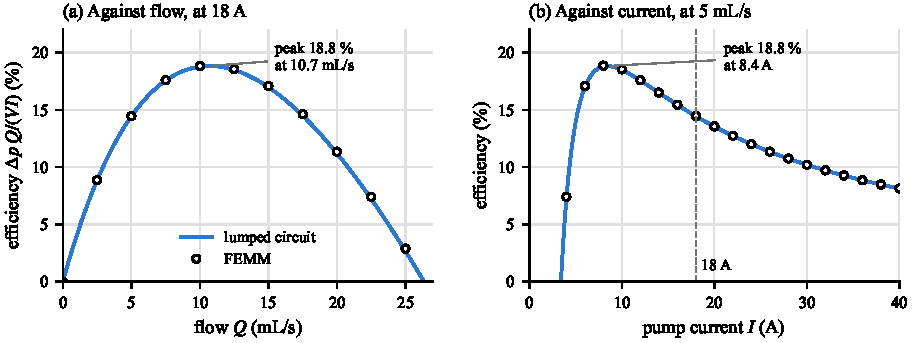
\includegraphics[width=\linewidth]{femm_efficiency}
  \caption{Modelled pump efficiency against flow and current.}
  \label{fig:femm-efficiency}
  \floatnote{\SI{20}{\milli\metre} electrodes, \SI{0.45}{\tesla}; terminal
    efficiency, excluding leads and contacts.}
\end{figure}

\begin{table}[htbp]
  \centering
  \caption{Main results of the FEMM pump model.}
  \label{tab:femm-results}
  \small
  \begin{tabular}{@{}lc@{}}
    \toprule
    Quantity & Value \\
    \midrule
    Electrode-to-electrode resistance & \SI{69.6}{\micro\ohm} \\
    Current inside the field & \SI{60}{\percent} \\
    Zero-flow pressure rise at \SI{18}{\ampere} & \SI{0.98}{\kilo\pascal} \\
    Efficiency at \SI{5}{\milli\litre\per\second}, \SI{18}{\ampere} & \SI{14.5}{\percent} \\
    Peak efficiency, \SI{20}{\milli\metre} electrodes & \SI{18.8}{\percent} \\
    Peak efficiency, \SI{60}{\milli\metre} electrodes & \SI{36.9}{\percent} \\
    Peak efficiency, \SI{20}{\milli\metre} electrodes,
      \SI{50}{\micro\ohm} series resistance & \SI{12.7}{\percent} \\
    \bottomrule
  \end{tabular}
  \floatnote{Terminal efficiency $\Delta p\,Q/(VI)$; the field covers the
    electrodes.}
\end{table}

The design studies suggest three ways to improve the pump. Lengthening the
electrodes, with the field lengthened to match, brings more of the current into
the field and roughly doubles the peak efficiency at \SI{60}{\milli\metre}.
Widening the channel adds flow area but not pressure unless the field is
lengthened with it. A shallower channel gives more pressure per ampere, but at
the cost of higher viscous loss.

The model also points to a likely cause of the low measured efficiency. The
measured pump power of \SI{0.85}{\watt} at \SI{18}{\ampere} corresponds to a
terminal resistance of about \SI{2.6}{\milli\ohm}, nearly 40 times the
\SI{69.6}{\micro\ohm} of the modelled channel and electrodes. Most of the input
power is therefore likely dissipated in the leads, joints and
electrode--Galinstan contacts, which the model does not include. Because the
pump itself is only tens of microohms, even \SI{50}{\micro\ohm} of series
resistance reduces its peak efficiency by about a third
(\cref{tab:femm-results}), so the supply should sit next to the pump on short,
heavy busbars.

\section{Work Remaining}

The model is two-dimensional, so the top and bottom walls, Hartmann layers and
the real velocity profile are not captured, and it assumes a uniform field with
sharp edges, nominal room-temperature conductivities and ideal contacts. To be
used for design, it would need to be validated against measurements of the
pump's pressure--flow curve and terminal voltage, extended to include the
contact and lead resistances and the fringing of the magnet field, and coupled
to the pressure drop of the cooling loop to find the operating point.


\end{document}
"
% =====================================================================
\documentclass[11pt,a4paper,twoside,openany]{report}

% The report class has no \frontmatter, \mainmatter or \backmatter (the book
% class does). Define them as in book.cls for the roman/arabic page numbering:
% with openany they start a new page, with openright a new odd page.
\makeatletter
\providecommand{\frontmatter}{%
  \if@openright\cleardoublepage\else\clearpage\fi\pagenumbering{roman}}
\providecommand{\mainmatter}{%
  \if@openright\cleardoublepage\else\clearpage\fi\pagenumbering{arabic}}
\providecommand{\backmatter}{%
  \if@openright\cleardoublepage\else\clearpage\fi}
\makeatother

\newif\ifreview
\reviewfalse
\ifdefined\REVIEW \reviewtrue \fi

% ---------------------------------------------------------------------
%  Fonts, language and page geometry
% ---------------------------------------------------------------------
\usepackage[T1]{fontenc}
\usepackage[utf8]{inputenc}
\usepackage{lmodern}                 % Computer Modern in T1 (as in Lawton)
\usepackage[british]{babel}          % NZ/UK spelling and hyphenation
\usepackage{microtype}
% Compact layout: narrow margins and near-single spacing, so that the body
% (Introduction to Conclusion) fits within 30 pages.
\usepackage[a4paper,top=20mm,bottom=20mm,inner=20mm,outer=20mm,
            headheight=14pt,headsep=6mm,footskip=10mm]{geometry}
\usepackage{setspace}
\setstretch{1.05}
\setlength{\emergencystretch}{1.5em}

% Display faces used for the title page and chapter openers
\newcommand{\chapnumfont}{\fontfamily{ppl}\fontseries{b}\selectfont}  % Palatino bold
\newcommand{\titlefont}{\fontfamily{bch}\fontseries{b}\selectfont}    % Charter bold

% ---------------------------------------------------------------------
%  Maths, units, tables, figures
% ---------------------------------------------------------------------
\usepackage{amsmath,amssymb}
\usepackage{siunitx}
\sisetup{
  per-mode            = symbol,
  inter-unit-product  = \ensuremath{\cdot},
  range-phrase        = --,
  range-units         = single,
  list-final-separator= {, and },
  product-units       = single,
}
\usepackage{graphicx}
\graphicspath{{figures/}}
\usepackage{booktabs,tabularx,array,multirow,makecell,longtable}
\renewcommand{\arraystretch}{1.15}
\newcolumntype{L}{>{\raggedright\arraybackslash}X}
\newcolumntype{C}{>{\centering\arraybackslash}X}
\usepackage{xcolor}
\definecolor{uoablue}{RGB}{0,70,127}
\usepackage{enumitem}
\setlist{itemsep=0pt,topsep=4pt}
\usepackage[labelsep=colon,skip=6pt]{caption}
\captionsetup[table]{position=top}
% All captions flush left, so short and long captions (and the notes below
% them) line up the same way.
\captionsetup{singlelinecheck=false}
% Captions are a short title only. Any further detail goes in a concise note:
% under the caption of a figure, or under the body of a table. \tnote marks
% the table cell that a note refers to.
\newcommand{\floatnote}[1]{\par\vspace{3pt}%
  {\raggedright\footnotesize\textit{Note:} #1\par}}
\newcommand{\tnote}[1]{\textsuperscript{#1}}
\usepackage{float}
\usepackage{placeins}                % \FloatBarrier keeps floats in their section
% Float placement. With LaTeX's defaults most floats here ended up on sparse
% float-only pages, centred vertically, away from the text that cites them.
% Allow more and larger floats on text pages (floats use [htbp]), accept a
% float-only page only when it is at least 3/4 full, and stack the floats at
% the top of such a page instead of spreading them down it.
\setcounter{topnumber}{3}
\setcounter{bottomnumber}{2}
\setcounter{totalnumber}{4}
\renewcommand{\topfraction}{0.85}
\renewcommand{\bottomfraction}{0.6}
\renewcommand{\textfraction}{0.12}
\renewcommand{\floatpagefraction}{0.75}
% When a page with floats cannot be filled exactly (e.g. the next heading does
% not fit), open up the gap between the floats and the text rather than the
% spacing between paragraphs.
\setlength{\textfloatsep}{14pt plus 12pt minus 4pt}
\setlength{\floatsep}{10pt plus 4pt minus 2pt}
\setlength{\intextsep}{10pt plus 4pt minus 2pt}
\makeatletter
\setlength{\@fptop}{0pt}
\setlength{\@fpsep}{\floatsep}
\setlength{\@fpbot}{0pt plus 1fil}
\makeatother
\usepackage{pdfpages}                % signed statement of contribution
\usepackage{nomencl}                 % nomenclature (ECSE template)
\makenomenclature
\usepackage[titles]{tocloft}         % TOC/LOF/LOT entries as in the ECSE template

\usepackage{subcaption}
% Subfigures: centred "(a) ..." captions, cited as "Fig. 4.5(a)"
\captionsetup[sub]{singlelinecheck=true,labelformat=simple}
\renewcommand{\thesubfigure}{(\alph{subfigure})}
\usepackage{pgfplots}
 \pgfplotsset{compat=1.17}
\usepgfplotslibrary{groupplots}      % multi-panel transient figures
\usepackage[american]{circuitikz}    % thermal network figure

% ---------------------------------------------------------------------
%  Headings
% ---------------------------------------------------------------------
\usepackage{titlesec}
% Chapter heading: bold Computer Modern, flush left, number and title on one
% line at the top of the page (compact layout).
\newcommand{\bodychapterformat}{%
  \titleformat{\chapter}[hang]
    {\normalfont\LARGE\bfseries\raggedright}
    {\thechapter}
    {0.8em}
    {}%
  \titleformat{name=\chapter,numberless}[hang]
    {\normalfont\LARGE\bfseries\raggedright}
    {}
    {0pt}
    {}%
  \titlespacing*{\chapter}{0pt}{0pt}{16pt}}
\bodychapterformat
\titleformat{\section}{\normalfont\large\bfseries}{\thesection}{1em}{}
\titleformat{\subsection}{\normalfont\normalsize\bfseries}{\thesubsection}{1em}{}
\titleformat{\subsubsection}{\normalfont\normalsize\bfseries}{\thesubsubsection}{1em}{}
\titlespacing*{\section}{0pt}{2.2ex plus .8ex minus .2ex}{1.0ex plus .2ex}
\titlespacing*{\subsection}{0pt}{1.8ex plus .6ex minus .2ex}{0.8ex plus .2ex}
\titlespacing*{\subsubsection}{0pt}{1.6ex plus .6ex minus .2ex}{0.5ex plus .2ex}
\setcounter{secnumdepth}{2}
\setcounter{tocdepth}{2}

% Front-matter headings follow the ECSE template (14 pt bold, flush left);
% \bodyheadings restores the body chapter heading for the main matter.
\newcommand{\frontheadings}{%
  \titleformat{name=\chapter,numberless}[block]
    {\normalfont\fontsize{14}{17}\selectfont\bfseries}{}{0pt}{}%
  \titlespacing*{\chapter}{0pt}{0pt}{12pt}}
\newcommand{\bodyheadings}{\bodychapterformat}

% ---------------------------------------------------------------------
%  ECSE template settings for the front matter
% ---------------------------------------------------------------------
\newcommand\HRule{\noindent\rule{\linewidth}{2pt}}   % title-page rules
\addto\captionsbritish{\renewcommand{\contentsname}{Table of Contents}}
% "Figure"/"Table" prefixes in the lists of figures and tables
\renewcommand{\cftfigpresnum}{Figure~}
\renewcommand{\cfttabpresnum}{Table~}
\setlength{\cftfignumwidth}{5.2em}
\setlength{\cfttabnumwidth}{5.2em}
% Nomenclature: "Symbols" / "Greek Symbols" groups with a unit column
\renewcommand{\nomname}{Nomenclature}
\def\nompreamble{\addcontentsline{toc}{chapter}{\nomname}\markboth{\nomname}{\nomname}}
\renewcommand{\nomgroup}[1]{%
  \ifthenelse{\equal{#1}{A}}{\item[\textbf{Symbols}]}{%
  \ifthenelse{\equal{#1}{G}}{\item[\textbf{Greek Symbols}]}{}}}
\newcommand{\nomunit}[1]{\renewcommand{\nomentryend}{\hspace*{\fill}#1}}
\setlength{\nomlabelwidth}{2.6cm}
\usepackage{ifthen}

% ---------------------------------------------------------------------
%  Running heads (Lawton: bold, ruled; page number outside;
%  chapter title on even pages, section on odd pages)
% ---------------------------------------------------------------------
\usepackage{fancyhdr}
\renewcommand{\chaptermark}[1]{\markboth{#1}{#1}}
\renewcommand{\sectionmark}[1]{\markright{\thesection\ \ #1}}
\fancypagestyle{lawton}{%
  \fancyhf{}%
  \fancyhead[LE]{\bfseries\thepage}%
  \fancyhead[RE]{\bfseries\nouppercase{\leftmark}}%
  \fancyhead[LO]{\bfseries\nouppercase{\rightmark}}%
  \fancyhead[RO]{\bfseries\thepage}%
  \renewcommand{\headrulewidth}{0.4pt}}
\pagestyle{lawton}
% Chapter opening pages use the plain style; in the body, give them the same
% ruled running head as every other page.
\newcommand{\bodyplainstyle}{%
  \fancypagestyle{plain}{%
    \fancyhf{}%
    \fancyhead[LE]{\bfseries\thepage}%
    \fancyhead[RE]{\bfseries\nouppercase{\leftmark}}%
    \fancyhead[LO]{\bfseries\nouppercase{\rightmark}}%
    \fancyhead[RO]{\bfseries\thepage}%
    \renewcommand{\headrulewidth}{0.4pt}}}
% ECSE template: no header, small centred page number
\fancypagestyle{front}{%
  \fancyhf{}%
  \fancyfoot[C]{\footnotesize\thepage}%
  \renewcommand{\headrulewidth}{0pt}}
\newcommand{\frontplainstyle}{%
  \fancypagestyle{plain}{%
    \fancyhf{}%
    \fancyfoot[C]{\footnotesize\thepage}%
    \renewcommand{\headrulewidth}{0pt}}}

% ---------------------------------------------------------------------
%  References (IEEE, with DOIs as in Lawton; source: Zotero export)
% ---------------------------------------------------------------------
\usepackage{csquotes}
\usepackage[backend=biber,style=ieee,
            doi=true,url=true,isbn=false,dashed=false,maxnames=6,minnames=1]{biblatex}
\addbibresource{zotero_references.bib}
\AtEveryBibitem{\clearfield{issn}%
  % an access date means nothing without a URL (e.g. Zotero items with no link)
  \iffieldundef{url}{\clearfield{urlyear}\clearfield{urlmonth}\clearfield{urlday}}{}}
% zotero_references.bib is the Zotero export; tidy its fields here rather than
% editing the file, so the fixes survive a refresh from Zotero. Drop language
% tags, ISBNs and the "ISSN: ..." notes Zotero writes, and give items that have
% a DOI only the DOI (no URL or access date).
\DeclareSourcemap{
  \maps[datatype=bibtex]{
    \map{
      \step[fieldset=language, null]
      \step[fieldset=isbn, null]
      \step[fieldsource=note, match=\regexp{\AISSN:}, final]
      \step[fieldset=note, null]
    }
    \map{
      \step[fieldsource=doi, final]
      \step[fieldset=url, null]
      \step[fieldset=urldate, null]
    }
    % Zotero stores an article number (e.g. 100133) as the page range; print it
    % as "Art. no." rather than as a page number
    \map{
      \pertype{article}
      \step[fieldsource=pages, notmatch=\regexp{-}, final]
      \step[fieldset=eid, origfieldval]
      \step[fieldset=pages, null]
    }
  }
}
\DeclareFieldFormat[article]{eid}{Art\adddot\space no\adddot\space#1}
% Some Zotero titles carry a zero-width space (U+200B), which pdfLaTeX cannot
% typeset; drop it here so the fix survives a refresh from Zotero. Also allow a
% line break after a Unicode em dash (U+2014), so that long titles such as
% Ouyang's do not run into the margin.
\DeclareUnicodeCharacter{200B}{}
\DeclareUnicodeCharacter{2014}{\textemdash\allowbreak}
% Break long DOIs and URLs without stretching the gaps around "." and "/"
\setcounter{biburlnumpenalty}{9000}
\setcounter{biburlucpenalty}{9000}
\setcounter{biburllcpenalty}{9000}
\biburlbigskip=0mu plus 1mu\relax

% ---------------------------------------------------------------------
%  Cross-referencing
% ---------------------------------------------------------------------
\usepackage[hidelinks,bookmarksnumbered]{hyperref}
\usepackage[nameinlink]{cleveref}
\crefname{chapter}{Chapter}{Chapters}
\crefname{section}{Section}{Sections}
\crefname{subsection}{Section}{Sections}
\crefname{figure}{Fig.}{Figs.}
\Crefname{figure}{Figure}{Figures}
\crefname{table}{Table}{Tables}
\crefname{appendix}{Appendix}{Appendices}
\crefname{subappendix}{Appendix}{Appendices}
\crefname{equation}{}{}
\crefformat{equation}{(#2#1#3)}
\crefrangeformat{equation}{(#3#1#4)--(#5#2#6)}
\crefmultiformat{equation}{(#2#1#3)}{ and~(#2#1#3)}{, (#2#1#3)}{ and~(#2#1#3)}

% ---------------------------------------------------------------------
%  Review notes
% ---------------------------------------------------------------------
\ifreview
  \usepackage[colorinlistoftodos,textsize=small]{todonotes}
    \newcommand{\issue}[1]{\par\todo[inline,color=orange!20,bordercolor=orange!70!black,
      linecolor=orange!70!black,caption={\textsc{Issue}: #1}]{\textbf{Issue:} #1}}
  \newcommand{\edited}[1]{\par\todo[inline,color=cyan!12,bordercolor=cyan!50!black,
      linecolor=cyan!50!black,caption={\textsc{Edited}: #1}]{\textbf{Edited:} #1}}
\else
  \newcommand{\issue}[1]{\ignorespaces}
  \newcommand{\edited}[1]{\ignorespaces}
\fi
% A value or detail still to be supplied. Always shown, in red, so that it
% cannot be missed in a submitted copy.
\newcommand{\missing}[1]{\textcolor{red}{[#1]}}
% \figureorplaceholder[options]{file}: as \includegraphics, but while
% figures/<file> does not exist yet it draws a framed placeholder naming the
% file, so the report still compiles.
\newcommand{\figureorplaceholder}[2][]{%
  \IfFileExists{figures/#2}{\includegraphics[#1]{#2}}{%
    \fbox{\parbox[c][4cm][c]{0.85\linewidth}{\centering
      \missing{Figure to be added: figures/\detokenize{#2}}}}}}

% ---------------------------------------------------------------------
%  Convenience macros
% ---------------------------------------------------------------------
\newcommand{\Vdot}{\dot{V}}
\newcommand{\mdot}{\dot{m}}
\newcommand{\cp}{c_{\mathrm{p}}}
\newcommand{\NTU}{\mathrm{NTU}}
\newcommand{\Rcp}{R_{\mathrm{cp}}}
\newcommand{\Rpack}{R_{\mathrm{pack}}}
\newcommand{\Rmisc}{R_{\mathrm{misc}}}
\newcommand{\Qin}{Q_{\mathrm{in}}}
\newcommand{\Qplate}{Q_{\mathrm{plate}}}
\newcommand{\Tin}{T_{\mathrm{in}}}
\newcommand{\Tout}{T_{\mathrm{out}}}
\newcommand{\Tres}{T_{\mathrm{resistor}}}
\newcommand{\Galinstan}{Galinstan}
\newcommand{\GaInSn}[3]{Ga\textsubscript{#1}In\textsubscript{#2}Sn\textsubscript{#3}}

% ---------------------------------------------------------------------
%  Report details (edit here)
% ---------------------------------------------------------------------
\newcommand{\reporttitle}{Liquid Metal Cooling for High-Power-Density Power Electronic Converters}
\newcommand{\reportauthor}{Alex Skilton}
\newcommand{\reporttype}{Final Report}
\newcommand{\reportdate}{\number\day\ \ifcase\month\or January\or February\or March\or April\or May\or June\or July\or August\or September\or October\or November\or December\fi\ \number\year}
\newcommand{\reportpartner}{Shrirang Ekbote}
\newcommand{\reportsupervisor}{Dr. Patrick Lawton and Prof. Grant Covic}

\hypersetup{pdftitle={\reporttitle},pdfauthor={\reportauthor}}

% =====================================================================
\begin{document}

\frontmatter
\frontheadings
\frontplainstyle
\pagestyle{empty}
%% =====================================================================
%  Title page -- 2026 ECSE Part IV Final Report template
%  (layout, rules, sizes and logo as in mainDocument.tex of the template;
%  type sizes are fixed at the template's 12 pt values)
% =====================================================================
\begin{titlepage}
\newgeometry{top=2cm,bottom=2cm,left=2.5cm,right=2.5cm}
\begin{spacing}{1}
\fontsize{12}{14.5}\selectfont
\setlength{\parindent}{0pt}
\setlength{\parskip}{\medskipamount}

\vspace*{10mm}

\begin{center}
\textbf{\fontsize{14.4}{18}\selectfont Research Project Report}
\end{center}

\vspace*{10mm}

\HRule
\begin{center}
\reporttype
\end{center}

\begin{center}
\textbf{\fontsize{17.28}{22}\selectfont \reporttitle}
\end{center}

\begin{center}
{\fontsize{14.4}{18}\selectfont \reportauthor}
\end{center}

\HRule

\vspace*{\fill}

\begin{center}
\begin{tabular}{rl}
Partner:  & \reportpartner \\
\noalign{\vskip1.5em}
Supervisor: & \reportsupervisor \\
\noalign{\vskip1.5em}
\end{tabular}
\end{center}

\vspace*{\fill}

\begin{center}
\reportdate
\end{center}

\vspace*{\fill}

\begin{center}

\includegraphics[width=0.7\linewidth]{UoA-Logo-Primary-RGB-Large}
\end{center}

\end{spacing}
\restoregeometry
\end{titlepage}


\pagestyle{front}
%% =====================================================================
%  Abstract page -- ECSE template layout
% =====================================================================
\thispagestyle{front}
\begingroup
\setlength{\parindent}{0pt}
\setlength{\parskip}{9pt}

\vspace*{1em}

\begin{center}
\textbf{\large \MakeUppercase{\reporttitle}}
\end{center}

\vspace{2em}

\begin{center}
\textbf{\large \reportauthor}
\end{center}

\vspace{2em}

\begin{center}
\textbf{\large ABSTRACT}
\end{center}

% Write your abstract here
[Abstract to be written.]
% end of Abstract

\endgroup
\clearpage


% Signed Statement of Contribution (student + supervisor). Replace
% frontmatter/Declaration.pdf with the signed copy.
% 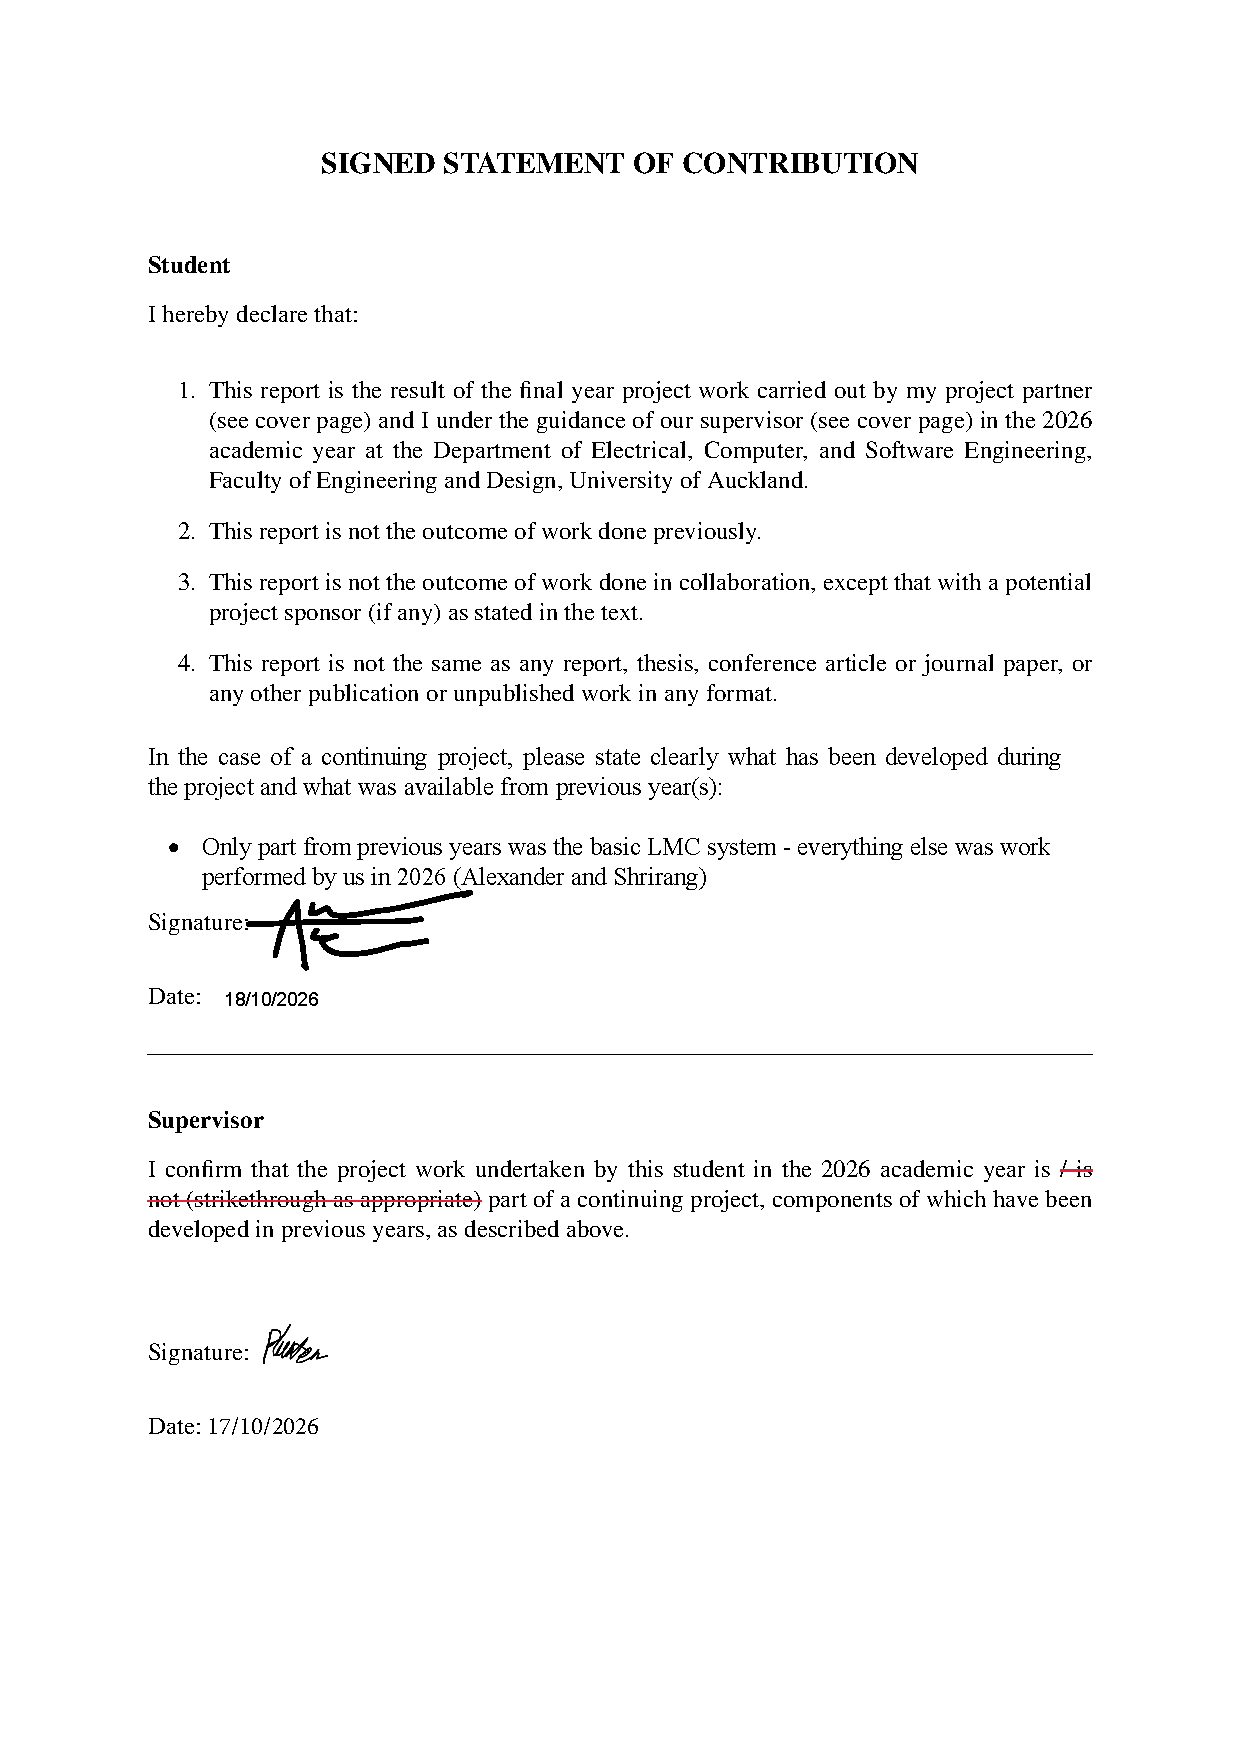
\includepdf[pagecommand=\thispagestyle{front}]{frontmatter/Declaration PAT SIGNED}
% \tableofcontents
% \listoffigures
% \listoftables
% % =====================================================================
%  Acknowledgements -- ECSE template
% =====================================================================
\chapter*{Acknowledgements}
\addcontentsline{toc}{chapter}{Acknowledgements}
\begingroup
\setlength{\parindent}{0pt}
\setlength{\parskip}{9pt}

Firstly, I would like to acknowledge my parents for their consistent love and support throughout my studies.

I would also like to express my sincere appreciation to my friend and project partner, Shrirang Ekbote, for his contributions, teamwork, and companionship throughout this project. It has been a long yet rewarding final year at university, and I look forward to continuing our journey together out in the professional world.

Thank you to my supervisors, Dr. Patrick Lawton and Professor Grant Covic, for their dedicated support, guidance, and expertise throughout this project. I truly appreciated your honest feedback and the time you took out of your busy schedules to encourage us when motivation was low. The lessons from this experience have undoubtedly made me a better engineer, and I will carry them with me into the future.

I would like to thank Cody Liu, Thor Bridger, Taha Basar, Howard Lu and the rest of the ECSE Power Electronics Lab for always being willing to help and contributing to a safe and functioning lab environment. 

Finally, thank you to all my other friends in the rest of the department and beyond, for contributing to the conversations, jokes, and memories throughout this year.

\endgroup

% % =====================================================================
%  Glossary of Terms -- ECSE template (Term / Definition longtable)
%  Definitions follow the usage in the report body; edit as needed.
% =====================================================================
\chapter*{Glossary of Terms}
\addcontentsline{toc}{chapter}{Glossary of Terms}

\begin{longtable}[l]{>{\raggedright}p{0.25\textwidth}>{\raggedright\arraybackslash}p{0.68\textwidth}}
\textbf{Term} & \textbf{Definition} \\
\addlinespace
Caloric resistance & Coolant temperature rise per unit heat load, $1/(\rho\,\cp\,\Vdot)$; the part of the thermal resistance set by the coolant's heat-capacity rate. \\
\addlinespace
Cold plate & Metal plate with internal coolant passages onto which heat-dissipating components are mounted. \\
\addlinespace
Conduction pump & Electromagnetic pump that drives a conductive liquid by passing a DC current through it across a magnetic field, producing a Lorentz force. \\
\addlinespace
Eddy current & Current induced in a conductor by a time-varying magnetic field, dissipating power as heat. \\
\addlinespace
Effectiveness & Ratio of the heat actually absorbed by the coolant to the maximum possible for the given inlet and wall temperatures. \\
\addlinespace
Galinstan & Eutectic gallium--indium--tin alloy that is liquid at room temperature. \\
\addlinespace
Power density & Power processed by a converter per unit volume. \\
\addlinespace
Skin depth & Depth at which an alternating current or field in a conductor has decayed to $1/e$ of its surface value. \\
\addlinespace
Thermal resistance & Temperature difference per unit heat flow between two points, in \si{\kelvin\per\watt}. \\
\end{longtable}
\addtocounter{table}{-1}

% % Abbreviations -- ECSE template layout (two-column longtable)
\chapter*{Abbreviations}
\addcontentsline{toc}{chapter}{Abbreviations}

\begin{longtable}[l]{>{\raggedright}p{0.25\textwidth}>{\raggedright\arraybackslash}p{0.68\textwidth}}
  AC    & Alternating current \\
  AI    & Artificial intelligence \\
  CAD   & Computer-aided design \\
  CHF   & Critical heat flux \\
  DC    & Direct current \\
  DCM   & Discontinuous conduction mode \\
  EM    & Electromagnetic \\
  EMF   & Electromotive force \\
  EV    & Electric vehicle \\
  Ga    & Gallium \\
  GaInSn & Gallium--indium--tin alloy (Galinstan) \\
  GaN   & Gallium nitride \\
  IPT   & Inductive power transfer \\
  LCC   & Inductor--capacitor--capacitor (compensation network) \\
  LCR   & Inductance--capacitance--resistance (meter) \\
  MHD   & Magnetohydrodynamic \\
  NaK   & Sodium--potassium alloy \\
  NTU   & Number of transfer units \\
  PEC   & Power electronic converter \\
  PFA   & Perfluoroalkoxy (polymer tubing) \\
  RQ    & Research question \\
  SiC   & Silicon carbide \\
  SMR   & Small modular reactor \\
  TIM   & Thermal interface material \\
  VA    & Volt-ampere \\
  ZVS   & Zero-voltage switching \\
\end{longtable}
\addtocounter{table}{-1}

% % Nomenclature (ECSE template: nomencl package, 'Symbols' and 'Greek Symbols'
% groups, unit in right-hand column). Prefix A = Symbols, G = Greek; the rest
% of the prefix is the sort key.

\nomenclature[Aa]{$A$}{Heat-transfer area of the cold-plate tube\nomunit{\si{\metre\squared}}}
\nomenclature[Ab]{$B$}{Magnetic flux density\nomunit{\si{\tesla}}}
\nomenclature[Actarget]{$C_{\mathrm{target}}$}{Target tuning capacitance\nomunit{\si{\farad}}}
\nomenclature[Acp]{$\cp$}{Specific heat capacity at constant pressure\nomunit{\si{\joule\per\kilogram\per\kelvin}}}
\nomenclature[Adh]{$D_{\mathrm{h}}$}{Hydraulic diameter\nomunit{\si{\metre}}}
\nomenclature[Ae]{$E$}{EMF measured by the flow sensor\nomunit{\si{\volt}}}
\nomenclature[Af]{$f$}{Frequency\nomunit{\si{\hertz}}}
\nomenclature[Ah]{$h$}{Convective heat transfer coefficient\nomunit{\si{\watt\per\metre\squared\per\kelvin}}}
\nomenclature[Ai1]{$I_{1}$}{Primary resonant current (rms)\nomunit{\si{\ampere}}}
\nomenclature[Ak]{$k$}{Thermal conductivity\nomunit{\si{\watt\per\metre\per\kelvin}}}
\nomenclature[Al]{$L$}{Heated tube length\nomunit{\si{\metre}}}
\nomenclature[Al1]{$L_{1}$}{Primary (inductor) self-inductance\nomunit{\si{\henry}}}
\nomenclature[Alg]{$l_{\mathrm{g}}$}{Air-gap length\nomunit{\si{\metre}}}
\nomenclature[Amdot]{$\mdot$}{Mass flow rate\nomunit{\si{\kilogram\per\second}}}
\nomenclature[An]{$N$}{Number of turns\nomunit{}}
\nomenclature[Anf]{$N_{\mathrm{f}}$}{Number of power cycles to failure\nomunit{cycles}}
\nomenclature[Anu]{Nu}{Nusselt number\nomunit{}}
\nomenclature[Antu]{NTU}{Number of transfer units, $hA/(\mdot\,\cp)$\nomunit{}}
\nomenclature[Ap]{$P$}{Tube perimeter\nomunit{\si{\metre}}}
\nomenclature[Aqqin]{$Q$, $\Qin$}{Heat load; input heat\nomunit{\si{\watt}}}
\nomenclature[Aqplate]{$\Qplate$}{Heat transferred into the cold plate\nomunit{\si{\watt}}}
\nomenclature[Arac]{$R_{\mathrm{ac}}$}{AC winding resistance\nomunit{\si{\ohm}}}
\nomenclature[Arcp]{$\Rcp$}{Cold-plate thermal resistance\nomunit{\si{\kelvin\per\watt}}}
\nomenclature[Armisc]{$\Rmisc$}{Thermal resistance to ambient\nomunit{\si{\kelvin\per\watt}}}
\nomenclature[Arpack]{$\Rpack$}{Package (resistor and interface) thermal resistance\nomunit{\si{\kelvin\per\watt}}}
\nomenclature[Are]{Re}{Reynolds number\nomunit{}}
\nomenclature[Ata]{$T_{\mathrm{A}}$}{Ambient temperature\nomunit{\si{\celsius}}}
\nomenclature[Atfx]{$T_{\mathrm{f}}(x)$}{Local coolant temperature\nomunit{\si{\celsius}}}
\nomenclature[Atintout]{$\Tin$, $\Tout$}{Coolant inlet and outlet temperatures\nomunit{\si{\celsius}}}
\nomenclature[Atj]{$T_{\mathrm{j}}$}{Junction temperature\nomunit{\si{\celsius}}}
\nomenclature[Atm]{$T_{\mathrm{M}}$}{Resistor (heat-source) node temperature\nomunit{\si{\celsius}}}
\nomenclature[Atp]{$T_{\mathrm{P}}$}{Isothermal plate node temperature\nomunit{\si{\celsius}}}
\nomenclature[Avdc]{$V_{\mathrm{DC}}$}{DC bus voltage\nomunit{\si{\volt}}}
\nomenclature[Avdot]{$\Vdot$}{Volumetric flow rate\nomunit{\si{\metre\cubed\per\second}}}
\nomenclature[Axres]{$X_{\mathrm{res}}$}{Resonant reactance\nomunit{\si{\ohm}}}
\nomenclature[Galphabeta]{$\alpha$, $\beta$}{Coffin--Manson fitting parameters\nomunit{}}
\nomenclature[Gdelta]{$\delta$}{Skin depth\nomunit{\si{\metre}}}
\nomenclature[Gdeltat]{$\Delta T$}{Temperature rise or swing\nomunit{\si{\kelvin}}}
\nomenclature[Gvarepsilon]{$\varepsilon$}{Cold-plate effectiveness\nomunit{}}
\nomenclature[Gmu]{$\mu$}{Dynamic viscosity\nomunit{\si{\pascal\second}}}
\nomenclature[Gmu0]{$\mu_{0}$}{Permeability of free space\nomunit{\si{\henry\per\metre}}}
\nomenclature[Grho]{$\rho$}{Density\nomunit{\si{\kilogram\per\metre\cubed}}}
\nomenclature[Gsigma]{$\sigma$}{Electrical conductivity\nomunit{\si{\siemens\per\metre}}}

% \printnomenclature
% \ifreview
%   \listoftodos[Review Notes]
% \fi

\clearpage{\pagestyle{empty}\cleardoublepage}% blank verso (if any) without a page number
\mainmatter
\bodyheadings
\bodyplainstyle
\pagestyle{lawton}
% =====================================================================
%  Chapter 1 -- Introduction (limited to one page)
% =====================================================================
\chapter{Introduction}
\label{ch:Introduction}

The continued electrification of the global economy is driving a sustained
increase in electricity demand~\cite{international_energy_agency_electricity_2025}.
Power electronic converters (PECs) enable this shift by electrifying
transport~\cite{bosshard_multi-objective_2016} and energy
systems~\cite{steimer_enabled_2010}. The power density of PECs has risen for decades,
driven by cost, functionality and hard weight and space
limits~\cite{steimer_enabled_2010,biela_cooling_2007}, and is projected to keep
rising~\cite{morroni_understanding_2023}. As converters shrink, however, the
same losses must be removed from a smaller volume, so thermal management
increasingly limits how far power density can
rise~\cite{biela_cooling_2007,morroni_understanding_2023}.

Inductive power transfer (IPT) chargers for electric vehicles illustrate this
challenge. At the standard \SI{85}{\kilo\hertz}~\cite{society_of_automotive_engineers_r_2024},
a \SI{10}{\kilo\watt} system dissipates several hundred watts, much of it in pads
that generate strong alternating magnetic fields~\cite{kim_thermal_2022}. Many
commercial designs already actively cool the coils~\cite{lawton_power_2024}, and
Liu \emph{et al.}\ call for new technologies to cool wireless
chargers~\cite{liu_thermal_2025}. Water cooling, however, is limited by the low
thermal conductivity of water~\cite{laloya_heat_2016}. Galinstan, a liquid metal
with much higher thermal conductivity~\cite{noauthor_gainsn_nodate}, can instead
be driven by a magnetohydrodynamic (MHD) pump with no moving
parts~\cite{hodes_potential_2014}, but its low volumetric heat capacity and
electrical conductivity bring trade-offs~\cite{hodes_potential_2014,an_liquid_2024}.
The extent of its advantage therefore remains unclear, as few studies compare it
with water at converter scale~\cite{fan_ultra-efficient_2026}.

This project builds on the 2025 Part~IV Project~\#51, in which Kwon and Loh
built an MHD-pumped Galinstan cooling loop and recommended comparing it with
water cooling and testing it near magnetic
components~\cite{kwon_project_2025,loh_project_2025}. Its aim is to evaluate
MHD-pumped Galinstan as a coolant for high-power-density PECs, and to identify
where in an IPT system it is most useful. The objectives are to (i)~compare the
thermal resistance and pumping power of the Galinstan loop with those of a water
loop using the same cold plate~\cite{ekbote_project_2026}; (ii)~explain and
extend the measurements with thermal models and a conjugate heat transfer
simulation; and (iii)~use a power-dense \SI{85}{\kilo\hertz} inductor to
demonstrate Galinstan cooling of magnetics and measure the eddy-current loss
induced in the coolant. These objectives are framed as two research questions
in \cref{sec:research-questions}. \Cref{ch:literature} reviews the literature,
\cref{ch:experimental} describes the methodology, \cref{ch:results} presents
the results, \cref{sec:discussion} discusses them and \cref{ch:conclusion}
concludes the report.

% =====================================================================
%  Chapter 2 -- Literature Review   (source: Literature_Review_Draft_v9.docx)
% =====================================================================
\chapter{Literature Review}
\label{ch:literature}
\edited{Section 2.3 restructured under three requirements (reliability, form
factor, efficiency), each comparing single-phase and phase-change cooling and
their implications for magnetic components. \Cref{tab:cooling-strategies} is
regrouped to match, with an added row for loss in magnetics.}

This chapter reviews the literature on cooling power electronic converters
(PECs) with liquid metal. It opens with the sources of loss in inductive power
transfer (IPT) systems, the application that motivates this work
(\cref{sec:ipt-losses}). It then presents the current trend that the power
density of PECs is increasing (\cref{sec:motivation}), and the reliability,
form-factor and efficiency requirements that their thermal management must meet,
which point to liquid metal cooling as a potential solution
(\cref{sec:thermal-management}). \Cref{sec:liquid-metal} evaluates this
proposal, and \cref{sec:research-gap} identifies the research gap and states
the research questions of this project.
\edited{The draft pointed to ``Section 2.6'' for the research gap; there is no
Section 2.6 (the gap is \cref{sec:research-gap}). All section, figure, table and
equation references are now generated with \texttt{\textbackslash cref}, so they
will stay correct if the structure changes.}

% ---------------------------------------------------------------------
\section{Thermal Losses in Inductive Power Transfer Systems}
\label{sec:ipt-losses}

IPT systems transfer power across a large air gap between loosely coupled
coils, and their losses are spread across the power electronics, the
compensation network and the magnetic pads. \Cref{fig:kim-losses} shows the
loss distribution that Kim \emph{et al.}\ measured and simulated for a
\SI{10}{\kilo\watt} IPT system with double-D (DD) pads, operating at
\SI{85}{\kilo\hertz} at a worst-case ambient temperature of
\SI{50}{\celsius}~\cite{kim_thermal_2022}. Most of the loss occurs in the pads,
chiefly in the Litz wire and ferrite, with smaller shares in the compensation
capacitors and in the aluminium shielding sheet, in which the leakage field
induces eddy currents. The inverter and rectifier dissipate about
\SIrange{70}{80}{\watt} each.

\begin{figure}[htbp]
  \centering
  \begin{tikzpicture}
    \begin{axis}[
      xbar stacked,
      width=0.78\linewidth, height=5.6cm,
      bar width=8pt,
      xmin=0, xmax=300,
      xlabel={Power loss (\si{\watt})},
      symbolic y coords={Inverter,Rectifier,Transformer,Cpi,Lsi,Secondary,Primary},
      ytick=data,
      yticklabels={Inverter, Rectifier, Transformer, $C_{\mathrm{pi}}$,
        $L_{\mathrm{si}}$, Secondary pad, Primary pad},
      tick label style={font=\small},
      label style={font=\small},
      xmajorgrids=true, grid style={dashed, gray!30},
      axis x line*=bottom, axis y line*=left,
      enlarge y limits=0.1,
      legend style={at={(0.98,0.04)}, anchor=south east, font=\small,
        draw=none, fill=white, fill opacity=0.85, text opacity=1},
      legend cell align=left,
    ]
      \addplot[fill=blue!60, draw=none] coordinates
        {(0,Inverter) (0,Rectifier) (0,Transformer) (0,Cpi) (0,Lsi) (40,Secondary) (165,Primary)};
      \addplot[fill=red!70, draw=none] coordinates
        {(0,Inverter) (0,Rectifier) (0,Transformer) (0,Cpi) (0,Lsi) (10,Secondary) (68,Primary)};
      \addplot[fill=green!55!black, draw=none] coordinates
        {(0,Inverter) (0,Rectifier) (0,Transformer) (0,Cpi) (0,Lsi) (12,Secondary) (39,Primary)};
      \addplot[fill=cyan!70, draw=none] coordinates
        {(0,Inverter) (0,Rectifier) (0,Transformer) (0,Cpi) (0,Lsi) (5,Secondary) (17,Primary)};
      \addplot[fill=brown!70, draw=none] coordinates
        {(80,Inverter) (70,Rectifier) (34,Transformer) (8,Cpi) (11,Lsi) (0,Secondary) (0,Primary)};
      \legend{Litz wire, Ferrite, Capacitors, Aluminium, Other components}
    \end{axis}
  \end{tikzpicture}
  \caption{Power loss distribution across a \SI{10}{\kilo\watt},
    \SI{85}{\kilo\hertz} IPT system with DD pads at an ambient temperature of
    \SI{50}{\celsius}, recreated from Kim \emph{et al.}~\cite{kim_thermal_2022}
    (values read from the original figure). $L_{\mathrm{si}}$ and $C_{\mathrm{pi}}$
    are components of the compensation network.}
  \label{fig:kim-losses}
\end{figure}

These losses differ in density. The pad losses are spread over about
\SI{0.8}{\metre} by \SI{0.6}{\metre} inside a strong alternating magnetic field,
and the pad is cooled passively, reaching a simulated peak temperature of about
\SI{96}{\celsius}. Its components also change with temperature: the Litz wire
resistance rises by about \SI{0.4}{\percent} per degree and the ferrite loss
varies nonlinearly, so power loss and temperature cannot be considered
separately~\cite{kim_thermal_2022}. The semiconductor losses, by contrast, are
concentrated in small switching devices placed away from the coupler. Where an
alternative coolant could be used in an IPT system therefore depends on both the
heat flux and the magnetic field the cooling system is exposed to, a question this report
returns to in \cref{sec:disc-suitability}.

Wireless charging of light-duty electric vehicles is standardised at a nominal
operating frequency of \SI{85}{\kilo\hertz}~\cite{society_of_automotive_engineers_r_2024},
the frequency used by Kim \emph{et al.}~\cite{kim_thermal_2022} and by
high-power IPT systems for public transport~\cite{bosshard_multi-objective_2016}.
The magnetic components of these systems are driven at this frequency, so any
cooling hardware placed near them is exposed to leakage fields at this
frequency. For this reason,
the power-dense inductor used in this work (\cref{sec:inductor-design}) is
operated at \SI{85}{\kilo\hertz}.
\issue{The Zotero record for SAE J2954 (\texttt{society\_of\_automotive\_engineers\_r\_2024})
has typos in its title (``J2594'', ``Vechicles''), which will print in the
reference list. Fix them in Zotero and re-export the bib file.}

% ---------------------------------------------------------------------
\section{Power Density in Power Electronic Converters}
\label{sec:motivation}

PECs switch semiconductor devices at high frequency and use passive components,
chiefly inductors, transformers and capacitors, to store and release energy in
each switching cycle and to filter the resulting
waveforms~\cite{morroni_understanding_2023}. Magnetic components, frequently the
largest passive devices, are difficult to scale and often restrict the
achievable power
density~\cite{biela_cooling_2007,morroni_understanding_2023,sullivan_size_2016};
with heat sinks, they account for the largest portion of a power solution's
size~\cite{biela_cooling_2007,morroni_understanding_2023}. Higher switching
frequencies, now practical with wide-bandgap devices~\cite{gao_modeling_2022},
permit smaller passive components because less energy is stored per
cycle~\cite{morroni_understanding_2023}, but losses limit this gain.

Friedli \emph{et al.}\ demonstrated this trade-off with \SI{10}{\kilo\watt}
rectifiers built for switching frequencies from \SI{72}{\kilo\hertz} to
\SI{1}{\mega\hertz}~\cite{friedli_essence_2014}. As the frequency rose, the
boost inductor shrank, but the efficiency fell almost linearly from
\SI{97.3}{\percent} to \SI{93}{\percent} as the switching losses grew. With
forced-air cooling, the growing heat sink cancelled the gain, so the power
density peaked at \SI{6.5}{\kilo\watt\per\deci\metre\cubed} near
\SI{350}{\kilo\hertz}, and \SI{1}{\mega\hertz} could not be air-cooled at all.
Only with water cooling did the power density keep rising, to
\SI{14.1}{\kilo\watt\per\deci\metre\cubed} at
\SI{1}{\mega\hertz}~\cite{friedli_essence_2014}. The cooling method therefore
sets the achievable power density, and as shrinking components raise the heat
flux~\cite{morroni_understanding_2023}, further size reduction requires cooling
methods that transfer more heat per unit area~\cite{biela_cooling_2007}.

% ---------------------------------------------------------------------
\section{Thermal Management of Power Electronic Converters}
\label{sec:thermal-management}

The thermal management of a power-dense PEC must meet three requirements. It
must keep the converter reliable, fit within its form factor, and do so
efficiently, without adding significant loss to the converter, including in
nearby magnetic components. The following sections consider each requirement
in turn, comparing the two established families of cooling: single-phase
cooling with air or water, and phase-change cooling by boiling or heat pipes.
\Cref{tab:cooling-strategies} summarises how each meets these
requirements~\cite{liu_thermal_2025,rahman_emerging_2024,laloya_heat_2016,mudawar_assessment_2001}.

\begin{table}[htbp]
  \centering
  \caption[Thermal management requirements and established cooling strategies]{Summary
    of how established cooling strategies meet the requirements for PEC thermal
    management. COP: coefficient of performance, the ratio of heat removed to
    cooling power consumed.}
  \label{tab:cooling-strategies}
  \small
  \begin{tabularx}{\linewidth}{@{}>{\raggedright\arraybackslash}p{3.0cm} L L@{}}
    \toprule
    Requirement & Single-phase (air, water) & Phase change (boiling, heat pipes) \\
    \midrule
    \multicolumn{3}{@{}l}{\textit{Reliability}} \\
    \quad Maximum temperature
      & Forced air: tens of \si{\watt\per\centi\metre\squared};
        water cold plate: hundreds of \si{\watt\per\centi\metre\squared};
        water microchannel: $\approx$\SI{1000}{\watt\per\centi\metre\squared}
      & Highest, but capped by CHF \\
    \quad Temperature swing
      & Fan speed or flow rate provides control input
      & Boiling-onset thermal shock; no control input when passive \\
    \addlinespace
    \multicolumn{3}{@{}l}{\textit{Form factor}} \\
    \quad Compactness
      & Air: bulky heat sink; water: compact at the device, pump and radiator remote
      & Smaller and lighter than single-phase \\
    \addlinespace
    \multicolumn{3}{@{}l}{\textit{Efficiency}} \\
    \quad Burden power
      & Fans (COP 10--100) or pump (COP 300--500); rises steeply as channels narrow
      & Low; often passive \\
    \quad Loss in magnetics
      & \multicolumn{2}{>{\raggedright\arraybackslash}p{0.62\linewidth}}{Any
        conductive cooling hardware in a leakage field incurs eddy-current loss} \\
    \bottomrule
  \end{tabularx}
\end{table}

\subsection{Reliability Requirement}
\label{sec:reliability}

Thermal management is required, above all, to keep increasingly power-dense
PECs reliable. Thermal stress causes over \SI{50}{\percent} of electronic
equipment failures~\cite{rahman_emerging_2024}, and power semiconductors, which
dominate the overall reliability of power converters, account for approximately
\SI{31}{\percent} of PEC failures~\cite{kalay_systematic_2025}. The
Coffin--Manson model relates the number of thermal cycles to failure of a
semiconductor device to its junction temperature
swing~\cite{kalay_systematic_2025,albarbar_thermal_2018}:
\begin{equation}
  N_{\mathrm{f}} = \alpha \left(\Delta T_{\mathrm{j}}\right)^{\beta},
  \label{eq:coffin-manson}
\end{equation}
where $N_{\mathrm{f}}$ is the number of power cycles (in thousands) to failure,
$\Delta T_{\mathrm{j}}$ is the junction temperature swing, and $\alpha$ and
$\beta$ are experimentally determined parameters~\cite{kalay_systematic_2025}.
This simplified form omits the absolute-temperature term, which becomes
significant mainly above about \SI{200}{\celsius}~\cite{kalay_systematic_2025}.
Magnetic components also fail under thermal
stress~\cite{biela_cooling_2007,mengesha_advanced_2025,li_review_2022,lawton_power_2024}.
For reliability, the cooling system must therefore hold the maximum temperature
of both semiconductors and magnetics below their operating limits, and suppress
the temperature swing.

Single-phase cooling meets both requirements to a degree. Natural convection,
the simplest scheme, is limited by the low heat transfer coefficient of
air~\cite{biela_cooling_2007}, and is the conventional way of cooling magnetic
components from their exposed surfaces. Gao \emph{et al.}'s passively cooled
planar inductor rose more than \SI{65}{\celsius} in temperature at
\SI{12}{\ampere} rms, whereas with an engineered conduction path to a
liquid-cooled cold plate (\cref{fig:gao-inductor}) the rise was less than
\SI{3}{\celsius}~\cite{gao_modeling_2022}. Forced air and liquid cooling raise
the achievable heat flux, and their fan speed or flow rate provides a control
input over the temperature swing. Their heat flux, however, is bounded by the
coolant~\cite{rahman_emerging_2024,laloya_heat_2016}. Phase-change cooling
absorbs latent heat and offers the highest heat
flux~\cite{laloya_heat_2016,mudawar_assessment_2001}. Above the critical heat
flux (CHF), however, vapour blocks liquid access to the surface and the device
temperature rises uncontrollably. CHF is difficult to predict, so the safety
margin it demands erodes this advantage~\cite{mudawar_assessment_2001}, and
passive phase-change schemes offer no control over the temperature swing.

\begin{figure}[tbp]
  \centering
  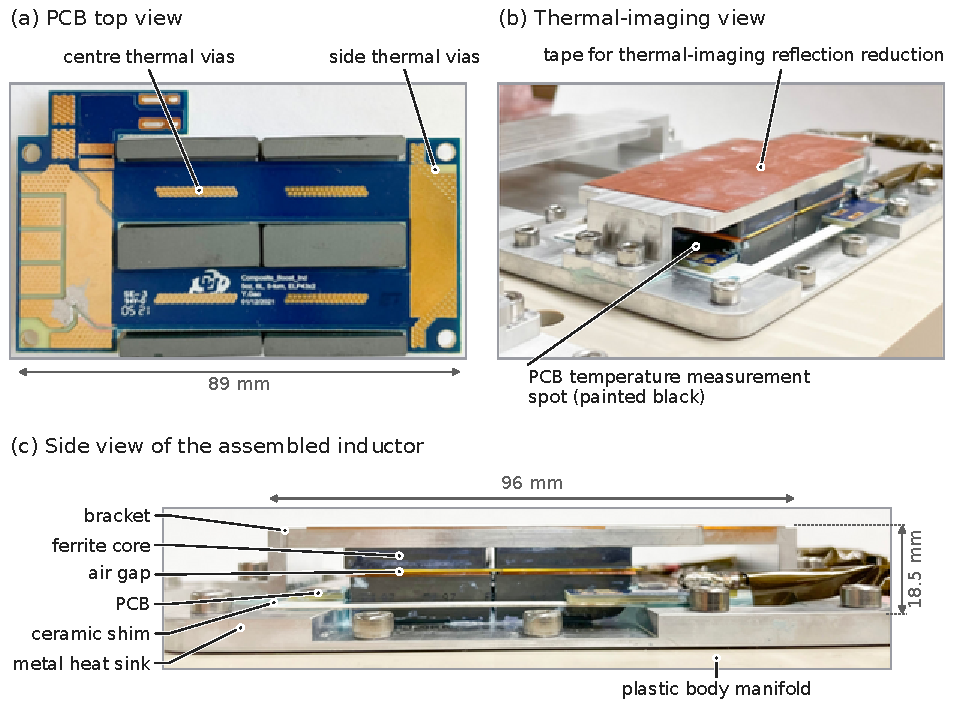
\includegraphics[width=0.75\linewidth]{gao_inductor_prototype}
  \caption[Planar inductor prototype of Gao \emph{et al.}]{Planar inductor
    prototype of Gao \emph{et al.} with an engineered conduction path to the
    cold plate: (a)~PCB top view; (b)~view used for thermal imaging;
    (c)~side view of the assembled inductor. Adapted
    from~\cite{gao_modeling_2022}.}
  \label{fig:gao-inductor}
\end{figure}

\subsection{Form Factor Requirement}
\label{sec:form-factor}

The cooling system must not erode the power density it is meant to enable. With
the magnetic components, heat sinks account for the largest portion of a power
converter's size, and in compact converters the thermal management system can
occupy a large share of the
volume~\cite{biela_cooling_2007,morroni_understanding_2023,friedli_essence_2014}.
Air cooling requires bulky heat sinks, which limited the power density of the
rectifiers of Friedli \emph{et al.}\ (\cref{sec:motivation}). Water cooling is
compact at the device, as the pump and radiator can be placed
remotely~\cite{friedli_essence_2014,laloya_heat_2016}, while phase-change
systems can be smaller and lighter still~\cite{laloya_heat_2016}. For magnetic
components, a compact cooling system must be placed as close as possible to the
windings, typically on both the top and bottom of the
core~\cite{krismer_accurate_2010,biela_cooling_2007}, which places it directly in
the component's leakage field.

\subsection{Efficiency Requirement}
\label{sec:efficiency-req}

To retain the efficiency of the converter, the power drawn by the cooling system,
its burden power, must remain small relative to the power
processed~\cite{laloya_heat_2016}, and the cooling hardware must not introduce
excessive loss into the converter. Single-phase cooling requires fans or pumps,
and raising its heat flux requires narrower channels, which raise the pressure
drop and pumping power steeply~\cite{rahman_emerging_2024,laloya_heat_2016}.
Single-phase cooling therefore trades the maximum temperature it can hold
against the burden power it draws. Phase-change cooling draws little or no
burden power, and is often passive~\cite{laloya_heat_2016}.

Cooling hardware placed near magnetic components, whether single-phase or
phase-change, sits in their leakage field and suffers eddy-current
loss~\cite{biela_cooling_2007,gao_modeling_2022,ouyang_overview_2014}. In Gao
\emph{et al.}'s design, the cold plate and bracket raised the measured AC winding
resistance by \SI{34}{\percent}~\cite{gao_modeling_2022}, and the aluminium
shielding sheet of an IPT pad dissipates about \SI{17}{\watt} in the same way
(\cref{fig:kim-losses})~\cite{kim_thermal_2022}. Biela and Kolar similarly found
that heat-transfer components near an inductor air gap must be recessed from
it~\cite{biela_cooling_2007}. Because magnetic components are present in most
converters~\cite{morroni_understanding_2023}, their leakage fields must be
considered in any PEC cooling design, even where the magnetics are not the main
thermal constraint.

No established scheme therefore meets all three requirements. Phase-change
cooling offers the highest heat flux at low burden power, but is capped by CHF
and offers no control over the temperature swing when passive. Single-phase
cooling is controllable, but its heat flux is bounded by the low thermal
conductivity of air and water, so a higher heat flux costs pumping power. A
coolant with substantially higher thermal conductivity could ease this trade-off
while keeping flow-rate control, which motivates much of the research into
liquid metal coolants~\cite{hodes_potential_2014}.

% ---------------------------------------------------------------------
\section{Liquid Metal as a Coolant}
\label{sec:liquid-metal}

Liquid metals have long been used as coolants where heat fluxes and operating
temperatures exceed those that conventional fluids can tolerate~\cite{rowinski_small_2015}. 
Much of the early characterisation of liquid metal cooling systems was carried out as fundamental research for nuclear
reactors~\cite{rowinski_small_2015}. These systems typically use lead or sodium
coolants, but lead is toxic and requires careful handling and
containment~\cite{oecd_handbook_2015}, whereas sodium is highly chemically
reactive, particularly with water and air, posing fire and explosion
hazards~\cite{foust_sodium-nak_1972}. These factors complicate broader commercial
deployment.

Liquid metal has more recently been proposed as a coolant for computing hardware and
PECs~\cite{fan_ultra-efficient_2026,zhang_water-based_2015}. The driving factor is its high thermal
conductivity, which promises high heat transfer rates~\cite{hodes_potential_2014,fan_ultra-efficient_2026,zhang_experimental_2019,zhang_investigation_2023}.
Such applications typically use gallium (Ga)-based eutectic alloys, the most
common being Galinstan (GaInSn), which is non-toxic and remains liquid at room temperature~\cite{hodes_potential_2014,an_liquid_2024}. 
Galinstan has a thermal conductivity of \SI{16.5}{\watt\per\metre\per\kelvin},
approximately 28 times that of water (\cref{tab:galinstan-properties}), which
enhances heat spreading and reduces temperature gradients~\cite{hodes_potential_2014,zhang_experimental_2019}. 
A Galinstan loop offers single-phase cooling, with no boiling limit to design around, and has the potential to
remove a higher heat flux than water~\cite{hodes_potential_2014, zhang_experimental_2019}.

These benefits come with significant trade-offs (\cref{tab:galinstan-properties}).
High density and viscosity raise pumping power and system weight. Because the
volumetric heat capacity is low, more than twice the flow of water is needed
for the same coolant temperature rise. Electrical conductivity rules out direct
contact with live parts and exposes the coolant to induction heating. 
The wide liquid range, by contrast, removes the CHF limit that
constrains phase-change cooling. The material cost is high, but at the
system level water and Galinstan are comparable because water pumps are
expensive~\cite{fan_ultra-efficient_2026}. Kwon~\cite{kwon_project_2025}
therefore concluded that liquid metal suits specialised applications where
efficiency, compactness and reliability justify its cost.

\begin{table}[htbp]
  \centering
  \caption{Selected properties and cost of the Galinstan used in this work
    (Rich Metals grade EU-10C, 68.5Ga--21.5In--10Sn by
    weight~\cite{noauthor_gainsn_nodate}) relative to water.}
  \label{tab:galinstan-properties}
  \small
  \begin{tabularx}{\linewidth}{@{}>{\raggedright\arraybackslash}p{3.2cm}
      >{\raggedright\arraybackslash}p{2.9cm} L >{\raggedright\arraybackslash}p{1.3cm}@{}}
    \toprule
    Property & Galinstan & Relative to water & Source \\
    \midrule
    Thermal conductivity & \SI{16.5}{\watt\per\metre\per\kelvin} & About 28 times higher & \cite{noauthor_gainsn_nodate} \\
    Density & \SI{6370}{\kilogram\per\metre\cubed} & More than six times higher & \cite{noauthor_gainsn_nodate} \\
    Dynamic viscosity & \SI{2}{\milli\pascal\second} & About 2 times higher & \cite{noauthor_gainsn_nodate} \\
    Specific heat capacity & \SI{366}{\joule\per\kilogram\per\kelvin} & About one-fourteenth & \cite{zhang_experimental_2019} \\
    Volumetric heat capacity & \SI{2.3}{\mega\joule\per\metre\cubed\per\kelvin} & 0.45 times, so about 2.2 times the flow for equal $\Delta T$ & \cite{noauthor_gainsn_nodate} \\
    Electrical conductivity & \SI{3.46e6}{\siemens\per\metre} & Conductor (deionised water: \SI{5.5e-6}{\siemens\per\metre}) & \cite{noauthor_gainsn_nodate} \\
    Melting and boiling points & \SI{10}{\celsius} and above \SI{1300}{\celsius} & Liquid above \SI{10}{\celsius}, so it can solidify in cold storage; boiling will not occur & \cite{noauthor_gainsn_nodate,hodes_potential_2014} \\
    Material cost & US\$200--2000/kg & Orders of magnitude higher & \cite{an_liquid_2024} \\
    \bottomrule
  \end{tabularx}
\end{table}

Much of the reviewed work on Galinstan and other Ga-based coolants focuses on
micro- and mini-channel heat sinks for electronics, typically for heat loads
from watts to hundreds of watts. It is unclear from the literature whether such
systems can be scaled up to the channel sizes and temperatures more typical of
PECs. For example, EV-charging PECs have power classes on the order of tens of
kilowatts for light-duty vehicles and are being standardised up to
\SI{1}{\mega\watt} for heavy-duty
vehicles~\cite{lawton_power_2024,liu_thermal_2025,abb_e-mobility_mcs1200_nodate}. Large liquid
metal systems have been realised for nuclear reactors~\cite{rowinski_small_2015},
but these use different metals, operate at much higher temperatures and are much
larger than even the most powerful PEC applications, although some work has
addressed power electronic
converters~\cite{fan_ultra-efficient_2026,fan_liquid_2021}.

% ---------------------------------------------------------------------
\subsection{Electromagnetic Pumping}
\label{sec:em-pumping}

The low volumetric heat capacity of Galinstan makes pumping demanding. For a
heat load $Q$ and coolant temperature rise $\Delta T$, the required volumetric
flow rate is
\begin{equation}
  \Vdot = \frac{Q}{\rho \, \cp \, \Delta T},
  \label{eq:flow-requirement}
\end{equation}
where $\rho$ is the coolant density and $\cp$ its specific heat capacity.
Galinstan therefore needs about 2.2 times the flow of water
(\cref{tab:galinstan-properties}), which is identified as the primary
bottleneck for liquid metal heat sinks~\cite{hodes_potential_2014,an_liquid_2024}.
Its high thermal conductivity partly offsets this, because it sustains high heat
transfer coefficients in wider channels with a lower pressure
drop~\cite{zhang_water-based_2015,an_liquid_2024}.

The electrical conductivity of Galinstan also allows it to be driven by
electromagnetic (EM) pumps with no moving parts, which are silent,
vibration-free and compact~\cite{hodes_potential_2014}. Previous Part~IV
projects used a permanent-magnet DC conduction
pump~\cite{kwon_project_2025,loh_project_2025}. In this pump, a current $I$
passed through the coolant perpendicular to a magnetic field of flux density
$B$ produces a Lorentz force density
$\mathbf{J}\times\mathbf{B}$~\cite{kwon_project_2025}. An approximation for the
pressure developed is
\begin{equation}
  \Delta p = \frac{B I}{h},
  \label{eq:mhd-pressure}
\end{equation}
where $h$ is the channel height parallel to
$\mathbf{B}$~\cite{loh_project_2025}. Pressure therefore scales directly with
current, so the flow can be modulated to suppress temperature
swing~\cite{an_liquid_2024}, and shallow channels with strong magnets are
favoured. The cost is operation at high current and low voltage
(\SIrange{1}{100}{\ampere}, \SIrange{0.01}{0.5}{\volt},
\SIrange{0.1}{50}{\watt}), with efficiencies of only about
\SIrange{6}{10}{\percent}~\cite{an_liquid_2024,hodes_potential_2014}. Even
so, a conduction pump has drawn less than \SI{15}{\percent} of the power of a
mechanical water pump for the same cooling performance~\cite{an_liquid_2024}.

Induction pumps instead induce current in the coolant through an alternating or
travelling field. They are larger and more complex, but they develop greater
force~\cite{an_liquid_2024}. The field can also come from the converter itself.
Fan \emph{et al.}\ integrated an MHD pump into an inductor, so that the flow
self-adjusts with converter load~\cite{fan_liquid_2021}. The cost is
eddy-current losses in the coolant~\cite{fan_ultra-efficient_2026}. EM pumps
are, however, generally reported as individual designs. Among liquid metal
systems developed for power electronics, only those of Fan
\emph{et al.}\ have been compared against an equivalent water
system~\cite{fan_liquid_2021,fan_ultra-efficient_2026}.

% ---------------------------------------------------------------------
\subsection{Compatibility with Electrical Equipment}
\label{sec:compatibility}

Commercial use of Galinstan raises three concerns: material safety, corrosion
and electromagnetic compatibility. Galinstan was developed as a non-toxic,
non-flammable replacement for mercury. Its negligible vapour pressure means it
poses no inhalation risk~\cite{hodes_potential_2014}. Gallium oxide can damage
the respiratory system at high airborne concentrations, but a closed loop
releases only minimal amounts~\cite{an_liquid_2024}. Prior prototypes managed
skin contact and spillage with gloves, eye protection and containment
trays~\cite{kwon_project_2025,loh_project_2025}.

Ga-based alloys corrode aluminium severely, and copper requires protection
above \SI{100}{\celsius}~\cite{an_liquid_2024}. Erosion at high flow velocities
and the effect on ductile metals remain unstudied~\cite{hodes_potential_2014}.
Plastics and nickel-plated metals~\cite{hodes_potential_2014}, as well as
ceramics such as aluminium nitride~\cite{an_liquid_2024}, are compatible.
Aluminium nitride is also both thermally conductive and electrically
insulating, though expensive~\cite{gao_modeling_2022}.

Electrically, the coolant is a conductor. A leak onto
energised circuitry is a direct short~\cite{hodes_potential_2014}. The loop also
galvanically connects every wetted part, so the EM pump supply can energise the
radiator and cold plate~\cite{kwon_project_2025}. There is also potential for nearby
magnetics to induce eddy currents in the coolant, though this has not been strictly explored in the literature
(\cref{sec:thermal-management})~\cite{an_liquid_2024, fan_ultra-efficient_2026}.
As a result, low-cost plastic piping suits low-field regions. 
Near magnetics, it may be preferable to shield the coolant with a more conductive material to reduce eddy losses.

% ---------------------------------------------------------------------
\section{Research Gap and Objectives}
\label{sec:research-gap}

\subsection{Research Gap}
\edited{Trimmed only. The two opening sentences (water cooling is bounded by
water's thermal conductivity; Galinstan's higher conductivity can improve heat
transfer, both cited to Hodes \emph{et al.}) repeated
\cref{sec:thermal-management,sec:liquid-metal} and were cut. The two closing
sentences of the second gap (most converters contain magnetics; a cooling
system that does not cool them must still tolerate their leakage fields) are
now made in \cref{sec:thermal-management} and are replaced by a back-reference.
In the first gap, ``which use different metals at much higher temperatures''
was cut, as \cref{sec:liquid-metal} already says so.}

This study aims to address two gaps identified in the literature.

The first is the lack of comparisons between water and liquid metal at the scale
of a converter's cooling loop. Most existing comparisons are made for micro- and
mini-channel heat
sinks~\cite{hodes_potential_2014,zhang_water-based_2015,zhang_experimental_2019,an_liquid_2024},
or lie at the scale of nuclear reactors~\cite{rowinski_small_2015}. This study
aims to quantify the
trade-offs of the Galinstan system (as designed
in~\cite{kwon_project_2025,loh_project_2025}) relative to a comparable water-cooling
system.

The second is the cooling of magnetic components with Galinstan. To the author's
knowledge, no study has demonstrated Galinstan cooling of a magnetic component,
such as a power-dense inductor, or quantified the eddy-current losses induced in
the coolant by its leakage field. Eddy-current losses have been assessed in AC
conduction pumps~\cite{fan_ultra-efficient_2026}, and an inductor has been used to drive a
pump~\cite{fan_ultra-efficient_2026,fan_liquid_2021}, but not to cool the inductor itself
directly. As argued in \cref{sec:thermal-management}, the coolant's loss in a
leakage field matters even where the coolant does not cool the magnetics.

This project addresses both gaps using the existing Galinstan loop of
Loh~\cite{loh_project_2025} and Kwon~\cite{kwon_project_2025}. The loop comprises a
permanent-magnet MHD pump, perfluoroalkoxy (PFA) tubing, a cold plate and a
fan-cooled radiator, and can remove up to a \SI{72}{\watt} resistive
load~\cite{kwon_project_2025,loh_project_2025}. The loop was not tested against water
in the same apparatus, and its experiments did not consider magnetics:
Loh~\cite{loh_project_2025} focused on switching devices because Galinstan was
unlikely to interfere with them, unlike magnetics, and Kwon~\cite{kwon_project_2025}
excluded direct integration and testing with magnetics because of time
limitations and uncertainty about electromagnetic interference. Both recommended
comparison with water cooling, and Kwon also recommended testing higher heat
loads and investigating the interaction with inductive pad
fields~\cite{kwon_project_2025,loh_project_2025}.
\edited{``This project was not tested against water'' referred to the previous
project's loop, not this project; reworded to ``The loop was not tested
\dots''.}

\subsection{Research Questions}
\label{sec:research-questions}

These gaps lead to two research questions.

\begin{description}[leftmargin=3.2em,labelwidth=2.6em,labelsep=0.6em,itemsep=4pt]
    \item[RQ1] At the same heat load, how do the thermal resistance and pumping
    power of the Galinstan loop compare with those of a similar conventional
    water loop?
    \item[H1] Galinstan's higher thermal conductivity will lower the convective
    resistance relative to water in the same cold plate. However, the total
    thermal resistance of the Galinstan loop will be higher than that of the
    water loop. Its low volumetric heat capacity and low flow rate give a
    caloric resistance comparable to the conduction resistance of the cold
    plate.
    \item[RQ2] Can the Galinstan loop cool a power-dense inductor while adding
    minimal loss to the existing aluminium cold plate, and how large is the
    eddy-current loss induced in the coolant?
    \item[H2] The Galinstan loop will have a cooling effect on the inductor above that of natural convection. 
    The increase in loss due to eddy-current loss induced in the coolant will be
    small compared to the loss of introducing the cold plate.
    The metal of the cold plate between the inductor and the coolant is
    several skin depths thick at \SI{85}{\kilo\hertz}. Additionally, the high-frequency field will not change the coolant flow
    measurably. 
\end{description}

% =====================================================================
%  Chapter 3 -- Methodology
%  Structure follows the Experimental Section of Kwon (2025): setup,
%  design, modelling, then the experimental procedure.
% =====================================================================
\chapter{Methodology}
\label{ch:experimental}

The following sections detail the methodology used to evaluate
magnetohydrodynamically pumped Galinstan as a coolant for PECs. Two objectives
guided the work. The first is to compare the thermal performance of the
Galinstan cooling loop with that of a similar water cooling loop under
equivalent operating conditions (RQ1). The second is to quantify the influence
of a high-frequency magnetic leakage field on the Galinstan coolant (RQ2).
\Cref{sec:setup} describes the experimental setup, including the two cooling
loops, the instrumentation and the safety considerations.
\Cref{sec:inductor-design} presents the design of the power-dense inductor used
as the heat source in the second experiment. \Cref{sec:thermal-model} develops
the thermal models used to interpret the measurements, and
\cref{sec:programme} gives the procedures for the two experiments.

% ---------------------------------------------------------------------
\section{Experimental Setup}
\label{sec:setup}

\subsection{Cooling System Overview}
\label{sec:loop-overview}

Two cooling loops were used in this project, one circulating Galinstan and the
other water. Both follow the arrangement shown in \cref{fig:cooling-loop}. A
pump drives the coolant through a cold plate that interfaces with the heat
source, and then through a fan-cooled radiator, where the heat is rejected to
the environment. A flow sensor in the hot line measures the coolant flow rate.

\begin{figure}[htbp]
  \centering
  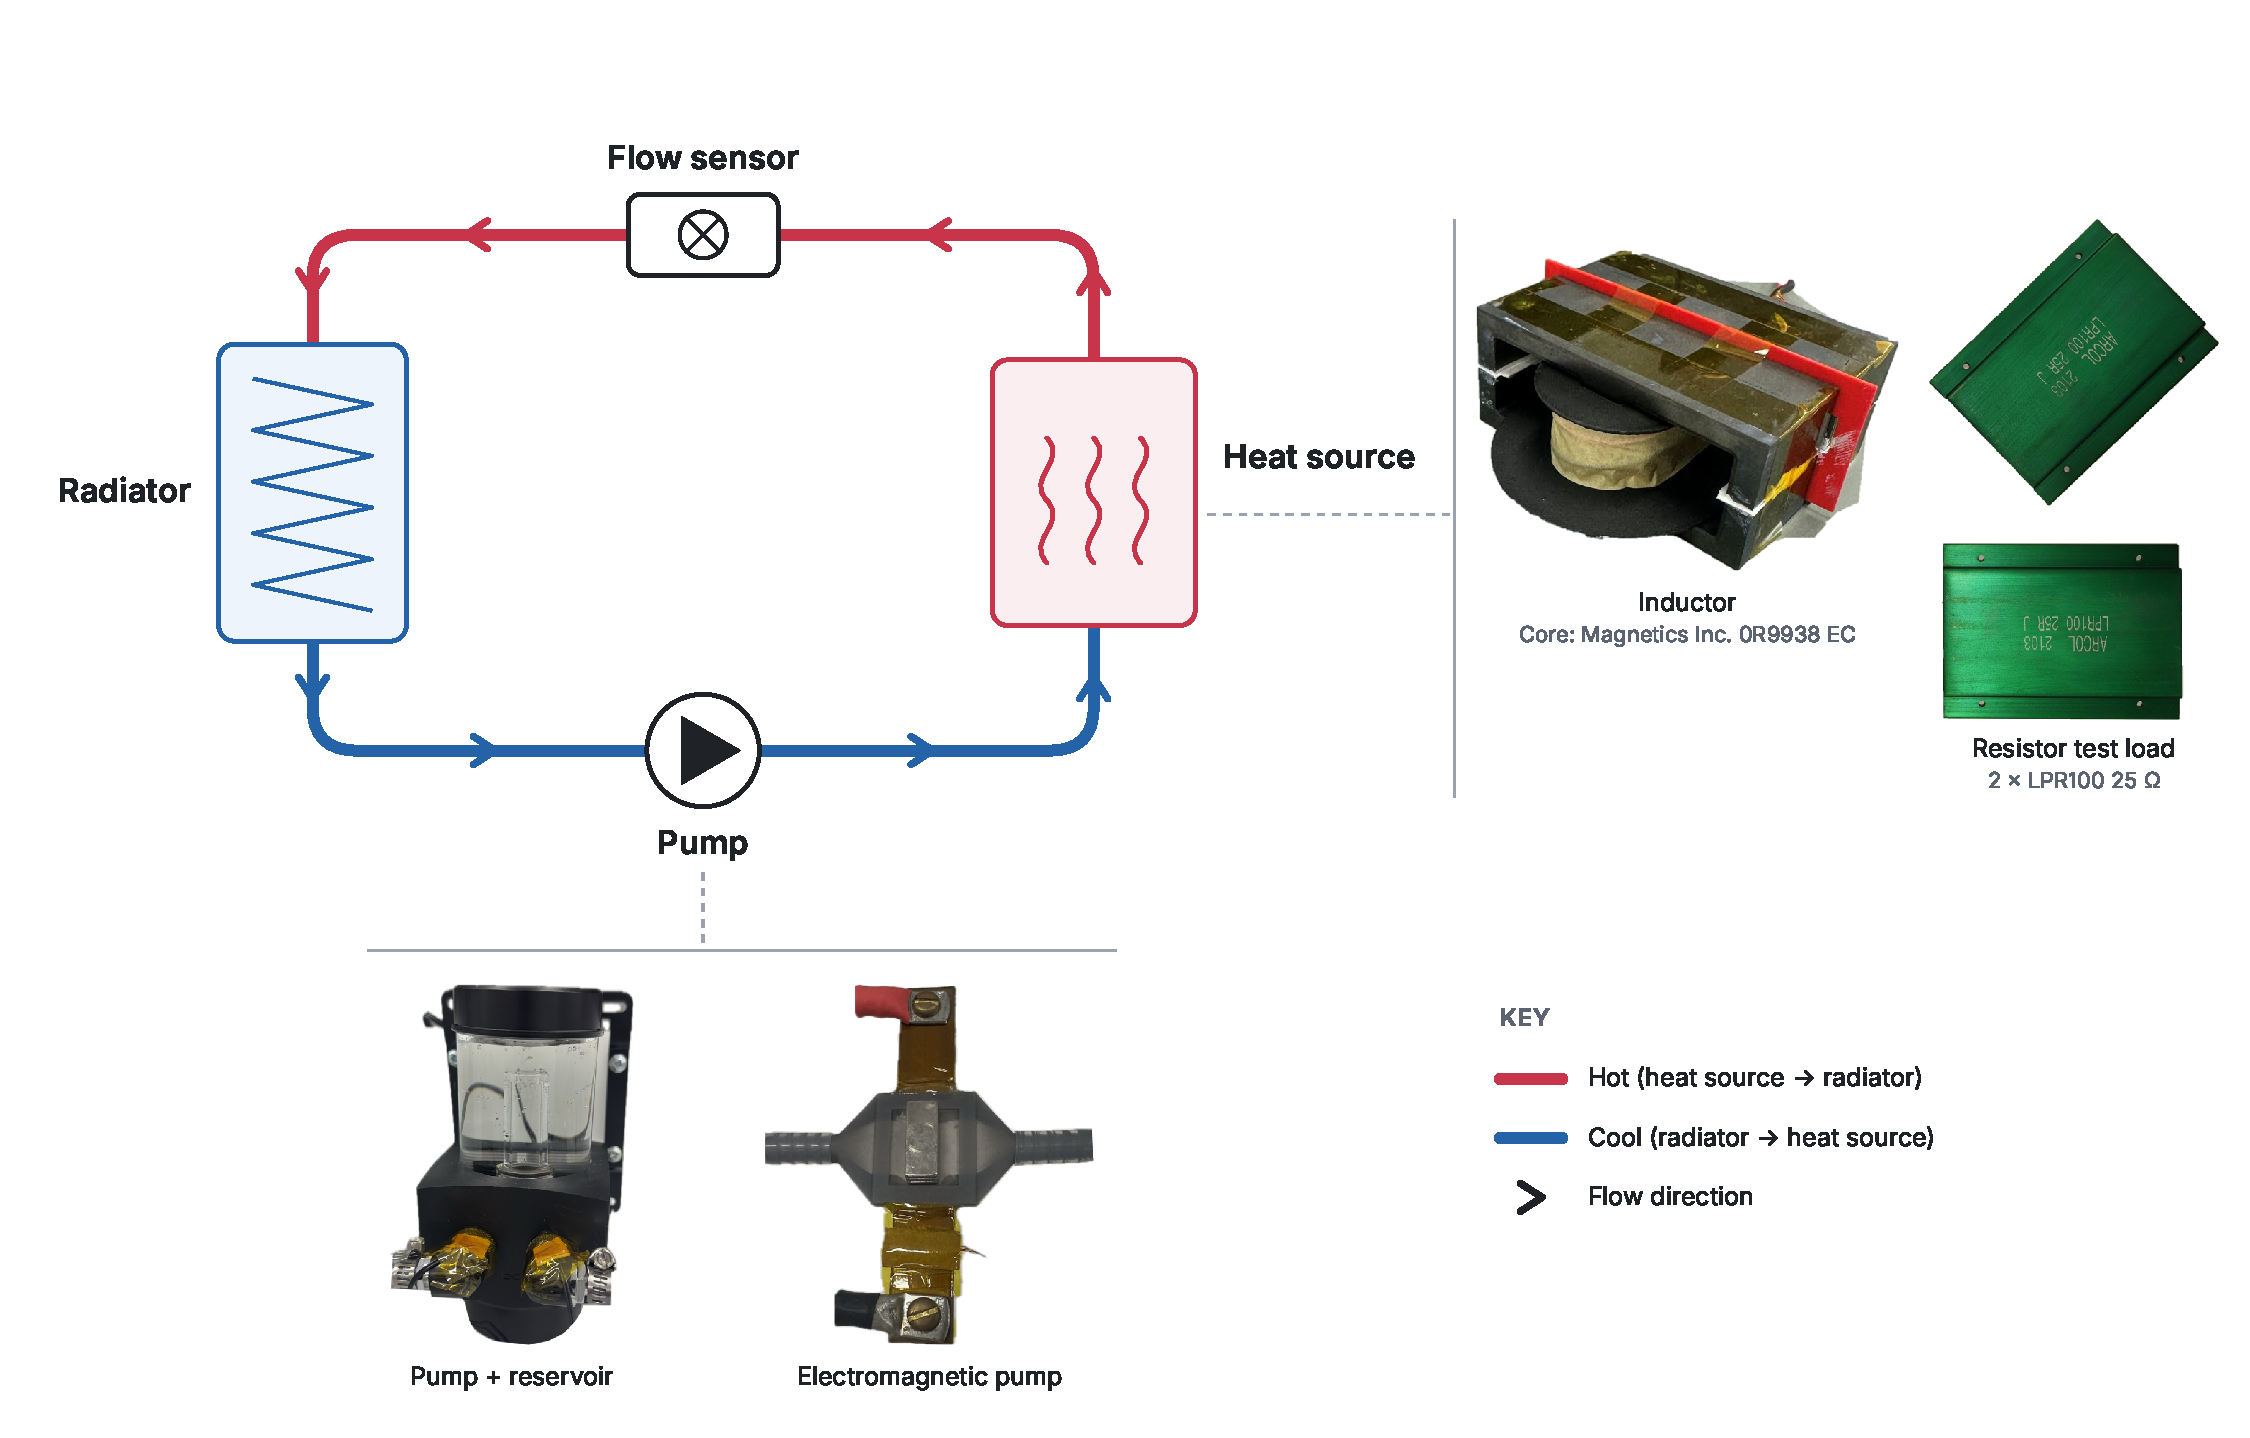
\includegraphics[width=0.85\linewidth]{figures/cooling_loop.pdf}
  \caption{Cooling loop arrangement shared by the Galinstan and water systems.
    The coolant is pumped through the heat source (resistor test load or
    inductor), past the flow sensor and through the radiator before returning
    to the pump. The water loop uses a pump with an integrated reservoir; the
    Galinstan loop uses an electromagnetic pump.}
  \label{fig:cooling-loop}
\end{figure}

The Galinstan loop is the apparatus constructed by the 2025 Part~IV Project~\#51
group~\cite{kwon_project_2025,loh_project_2025}. Galinstan is circulated by a
permanent-magnet DC conduction pump, in which a current passed through the
coolant between two copper electrodes produces a Lorentz force
(\cref{sec:em-pumping}). The pump is supplied by a XANTREX XKW~60--18 DC power
supply, which provides up to \SI{18}{\ampere}. PFA tubing carries the coolant
to an ATS-TCP-1001 tubed cold plate and back through an ATS-TCP-1003 cold plate
fitted with a heat sink and two fans, which acts as the
radiator~\cite{kwon_project_2025,advanced_thermal_solutions_inc_tubed_2021}.
Conventional mechanical flow meters are not compatible with Galinstan, so the
flow rate is measured with an electromagnetic flow sensor of the same
construction as the pump. The flowing coolant induces an EMF $E$ across the
sensor electrodes, from which the volumetric flow rate is $\Vdot = Eh/B$, where
$h$ is the channel height and $B$ the magnetic flux density across the
channel~\cite{kwon_project_2025}.

The water loop was designed and built by the project partner, Ekbote, to
replicate the Galinstan apparatus, and its design is detailed in Ekbote's
project report~\cite{ekbote_project_2026}. It uses the same model of tubed cold
plate (ATS-TCP-1001), so that the two
coolants are compared through an identical cold-plate geometry
(\cref{tab:coolant-properties}). The water is circulated by a pump with an
integrated reservoir, whose speed is set by the duty cycle of its drive signal,
and the flow rate is read directly from a Sea Zhongjiang digital flow meter. A
valve was later added to the water loop to reduce the flow below the
controllable range of the pump. The two loops therefore share the heat source
and the cold-plate geometry, but differ in the pump, the achievable flow range
and the method of flow measurement.

\subsection{Heat Sources}
\label{sec:heat-sources}

Two heat sources were used. For the first experiment, heat was applied by two
\SI{100}{\watt}, \SI{25}{\ohm} ARCOL LPR100 resistors mounted side by side on the
cold plate with a thermal interface material. The resistors were connected in
series and supplied by a GW Instek GPE-3323 DC power supply, so that the
dissipated power could be read directly from the supply. A heat load of
\SI{72}{\watt} (\SI{60}{\volt} across the \SI{50}{\ohm} pair) was used for most
tests, the same load used in~\cite{kwon_project_2025,loh_project_2025}. The
resistors were covered with polystyrene insulation to reduce the heat lost to
the environment. For the second experiment, the resistors were replaced by a
power-dense planar inductor, whose design is described in
\cref{sec:inductor-design}.

\subsection{Instrumentation}
\label{sec:instrumentation}

Galinstan is corrosive to many commonly used sensor materials, which restricts
the range of compatible measurement devices (\cref{sec:compatibility}). System
performance was therefore evaluated using the limited set of measurements
summarised in \cref{tab:measurements}. Temperatures around each loop were
logged continuously by a thermistor data-acquisition system adapted
from~\cite{kwon_project_2025,loh_project_2025}. At steady state, K-type
thermocouples, with an accuracy of $\pm\SI{2.2}{\celsius}$~\cite{loh_project_2025},
were used as the reference temperatures at the resistor, the cold-plate inlet
and the cold-plate outlet. A thermal camera was used where available, chiefly
for the inductor experiment.

\begin{table}[htbp]
  \centering
  \caption{Measured quantities and instrumentation.}
  \label{tab:measurements}
  \small
  \begin{tabularx}{\linewidth}{@{}>{\raggedright\arraybackslash}p{2.7cm}
      >{\raggedright\arraybackslash}p{4.1cm} L@{}}
    \toprule
    Quantity & Description & Method \\
    \midrule
    \multirow[t]{2}{=}{Heat load}
      & Power dissipated by the resistors.
      & Read from the GW Instek GPE-3323 DC power supply. \\
      & Power dissipated in the inductor.
      & Estimated from the core-loss model and the measured AC resistance
        (\cref{sec:model-validation}). \\
    \midrule
    \multirow[t]{2}{=}{Volumetric flow rate, $\Vdot$}
      & Galinstan loop.
      & EMF $E$ of the electromagnetic flow sensor, read with an Agilent 34410A
        digital multimeter; $\Vdot = Eh/B$~\cite{kwon_project_2025}. \\
      & Water loop.
      & Read directly from the Sea Zhongjiang digital flow meter. \\
    \midrule
    Temperature
      & Thermistors around the loop and, at steady state, thermocouples at the
        resistor, cold-plate inlet and cold-plate outlet.
      & Data-acquisition system adapted from~\cite{kwon_project_2025,loh_project_2025};
        thermal camera where available. \\
    \midrule
    Pump power
      & Electrical input power to each pump.
      & Voltage across the pump terminals and current from each pump's DC
        power supply. \\
    \midrule
    AC resistance, $R_{\mathrm{ac}}$
      & Series resistance of the inductor winding.
      & Agilent E4980A LCR meter (\cref{sec:exp2}). \\
    \midrule
    Pump volume
      & Volume occupied by each pump.
      & Physical measurement, supplemented by CAD dimensions where physical
        measurement is impractical. \\
    \bottomrule
  \end{tabularx}
\end{table}

\subsection{Safety Considerations}
\label{sec:safety}

The safety of project members and other laboratory users was prioritised
throughout the experimental setup and operation. Every experiment was set up by
two project members, and all connections were cross-checked with the project
partner before the system was energised. While temperatures exceeded
\SI{38}{\celsius}, the apparatus was continuously monitored by at least one
project member, and no one was permitted to interact with the system while it
was live. All electrical terminals operating above \SI{50}{\volt} DC were
covered, and the inverter and resonant tank used in the second experiment were
fully enclosed in acrylic boxes. Protective eyewear was worn, and physical
barriers prevented accidental contact with the live system. At shutdown, the
heat source was switched off first while the coolant continued to circulate,
and the apparatus was supervised for at least 30 minutes, until it had cooled
below \SI{38}{\celsius}.

% ---------------------------------------------------------------------
\section{Inductor Design}
\label{sec:inductor-design}

Cooling systems for magnetic components sit in their leakage fields
(\cref{sec:form-factor}), which could heat a Galinstan coolant. An initial ANSYS
simulation, with the Galinstan modelled as a stationary solid, found it 3.2
times as lossy as aluminium and almost 3.9 times as lossy as copper, and showed
that \SI{1}{\milli\metre} of copper shielding reduced the total loss by over
\SI{70}{\percent}. To measure this effect, a power-dense inductor that requires
active cooling was built and placed on the Galinstan cold plate. It operates at
\SI{85}{\kilo\hertz}~\cite{society_of_automotive_engineers_r_2024}, so that its
leakage field is representative of IPT magnetics (\cref{sec:ipt-losses}), and
uses a planar geometry, which offers better thermal performance than
alternatives such as pot cores. The final construction is shown in
\cref{fig:inductor-photo}.

\subsection{Analytical and Numerical Design}
\label{sec:analytical-design}

To reduce computation time and narrow the design space, an analytical model was
developed before the numerical simulations. This initial model assumed a
two-part construction of TDK N85 ferrite ELP-type cores, and swept the air-gap
length (\SIrange{0.5}{1.5}{\milli\metre}) and the number of turns (8--12). The
core loss of each design was estimated with the Steinmetz equation, which
expresses the loss per unit volume as a power law in frequency and peak flux
density~\cite{li_review_2022}. The model identified designs whose loss exceeds
the core's datasheet loss limit of
\SI{17.88}{\watt}~\cite{magnetics_inc_specification_2005}, so that active
cooling is required, while keeping the peak flux density below about
\SI{300}{\milli\tesla}.

An ANSYS model was then constructed and run as a two-parameter sweep over
air-gap length and number of turns. It was later found that the available cores
were Magnetics Inc.\ Material~R rather than the assumed TDK N85. A custom
material definition was therefore created by modifying the properties of TDK
N95, which are similar to those of Material~R. The core material was assumed to
operate at \SI{65}{\celsius}, the target steady-state operating temperature for
the experiments. With the material defined, a parameter sweep (8--12 turns,
\SIrange{0.5}{1.2}{\milli\metre} air gap) was performed to extract the
inductance and core loss.

To finalise the design, the flux density in the core was checked and found to
be acceptable, within the linear region of operation (\cref{fig:flux-density}).
The final design parameters, including the inductance and core loss of the
chosen design, are given in \cref{tab:inductor-design}.

\begin{figure}[htbp]
  \centering
  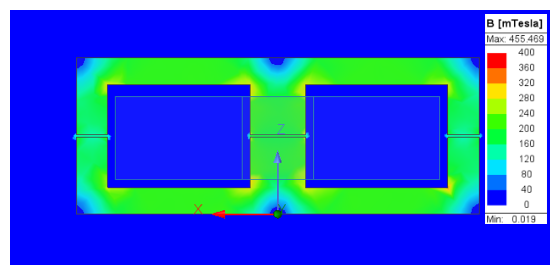
\includegraphics[width=0.72\linewidth]{inductor_flux_density}
  \caption{Magnetic flux density in the selected inductor design ($N = 8$,
    $l_{\mathrm{g}} = \SI{0.6}{\milli\metre}$).}
  \label{fig:flux-density}
\end{figure}

\begin{table}[htbp]
  \centering
  \caption{Final inductor parameters from the ANSYS model at the rated current
    of \SI{12}{\ampere} rms.}
  \label{tab:inductor-design}
  \begin{tabular}{@{}lll@{}}
    \toprule
    Parameter & Value & Unit \\
    \midrule
    Core geometry  & Magnetics Inc.\ 0\,9938\,EC & -- \\
    Core material  & Magnetics Inc.\ Material~R  & -- \\
    Air-gap length & 0.6   & \si{\milli\metre} \\
    Turns          & 8     & -- \\
    Inductance     & 92.5  & \si{\micro\henry} \\
    Core loss      & 30.81 & \si{\watt} \\
    \bottomrule
  \end{tabular}
\end{table}

\subsection{Model Validation}
\label{sec:model-validation}

Once the inductor had been built (\cref{fig:inductor-photo}), measurements were
taken to design the LCC tuning required to drive the desired resonant current.
These measurements also serve to validate the model, whose values at the rated
current of \SI{12}{\ampere} rms are given in \cref{tab:inductor-design}.

\begin{figure}[htbp]
  \centering
  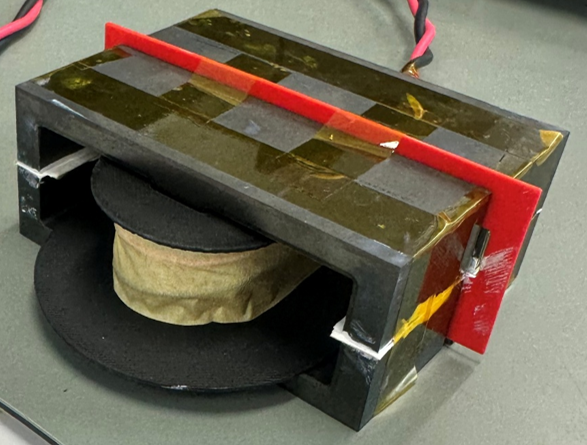
\includegraphics[width=0.42\linewidth]{inductor_photo}
  \caption{Constructed planar inductor.}
  \label{fig:inductor-photo}
\end{figure}

The inductance was measured as \SI{92.1}{\micro\henry}, within \SI{1}{\percent}
of the simulation model, although this measurement included the effect of long
leads, which would be expected to increase it. The AC resistance
$R_{\mathrm{ac}}$, which determines the winding loss, was measured with an LCR
meter at low excitation as \SI{83}{\milli\ohm}, giving a winding loss of
\SI{11.95}{\watt} at \SI{12}{\ampere} rms.

For a heat transfer investigation in which temperatures are continuously
monitored, some uncertainty in the loss estimate is acceptable. For the later
experiments, the total inductor loss is therefore taken as \SI{42.76}{\watt}
(\SI{30.81}{\watt} core loss plus \SI{11.95}{\watt} winding loss).

\subsection{Thermal Considerations and Cooling Strategy}
\label{sec:inductor-thermal}

The main constraint was asymmetric cooling. The upper core relies on convection
to ambient air, while the lower core sits on the cold plate, and the air gap
between them acts as a thermal insulator. Thermal paste was applied between the
upper and lower cores to reduce the temperature difference and improve heat
transfer to the cooling system. Although not optimal, this configuration is
suitable for the second experiment, which aims to demonstrate Galinstan cooling
of a power-dense inductor and to assess the leakage-field interaction rather
than to produce the best-performing system. Future work could improve the design
by cooling both the top and bottom cores, or by using asymmetric core designs
with an integrated heat-transfer path, such as the inductor of Gao
\emph{et al.}~\cite{gao_modeling_2022}.

\subsection{Capacitor Tuning}
\label{sec:capacitor-tuning}

The allowable reactance of the inductor was limited by the maximum voltage
developed across the series tuning capacitors needed to boost the volt-amperes
(VA) in the inductor, which was limited to \SI{150}{\volt} across any single
capacitor. To find
acceptable tuning values, an optimisation model was developed using the Solver
add-in in Microsoft Excel, which made it possible to check quickly whether a
given inductance was feasible or would cause the capacitor voltage to exceed its
rating.

The target capacitance is given by
\begin{equation}
  C_{\mathrm{target}} = \frac{1}{2\pi f \left(2\pi f L_{1} - X_{\mathrm{res}}\right)},
  \label{eq:c-target}
\end{equation}
where $f$ is the resonant frequency of the network (\SI{85}{\kilo\hertz}),
$L_{1}$ is the inductance of the primary magnetics and $X_{\mathrm{res}}$ is the
resonant reactance of the system. $X_{\mathrm{res}}$ sets the resonant current in
the primary magnetics, as given by
\begin{equation}
  X_{\mathrm{res}} = \frac{2\sqrt{2}\, V_{\mathrm{DC}}}{\pi I_{1}},
  \label{eq:x-res}
\end{equation}
where $I_{1}$ is the desired resonant current and $V_{\mathrm{DC}}$ is the DC bus
voltage, here \SI{60}{\volt}. \Cref{eq:x-res} is valid only for a conduction
angle of \SI{180}{\degree}. With the measured inductance of \SI{92.1}{\micro\henry} and a resonant current of
\SI{12}{\ampere}, \cref{eq:c-target,eq:x-res} give a target capacitance of
\SI{41.90}{\nano\farad}.

Initially, the optimisation model selected a single capacitor value for the
entire board. The result was relatively poor, with the best design differing by
\SI{8.11}{\percent} from the target capacitance. The model was then extended to
allow one value from a limited set (\SIlist{22;68;100}{\nano\farad}) to be
selected for each of the four series-connected rows of the tuning board, with up
to 14 capacitors in parallel per row. This reduced the detuning to
\SI{2.12}{\percent} of the target value. The final arrangement, with the voltage
across each row at the rated current, is given in \cref{tab:capacitor-opt}. The
highest row voltage is about \SI{146}{\volt}, within the \SI{150}{\volt} limit.

\begin{table}[htbp]
  \centering
  \caption{Final arrangement of the series tuning capacitors from the
    optimisation model. The four rows are connected in series; row voltages are
    at \SI{12}{\ampere} rms and \SI{85}{\kilo\hertz}.}
  \label{tab:capacitor-opt}
  \small
  \begin{tabular}{@{}lcccc@{}}
    \toprule
    Row & Capacitor value & Number in parallel & Row capacitance & Row voltage \\
        & (\si{\nano\farad}) & & (\si{\nano\farad}) & (\si{\volt}) \\
    \midrule
    1 & 22 & 7 & 154 & 145.9 \\
    2 & 68 & 3 & 204 & 110.1 \\
    3 & 22 & 7 & 154 & 145.9 \\
    4 & 22 & 7 & 154 & 145.9 \\
    \midrule
    \multicolumn{3}{@{}l}{Target capacitance}   & 41.90 & \\
    \multicolumn{3}{@{}l}{Achieved capacitance} & 41.01 & \\
    \multicolumn{3}{@{}l}{Error}                & 0.89 (\SI{2.12}{\percent}) & \\
    \bottomrule
  \end{tabular}
\end{table}

% ---------------------------------------------------------------------
\section{Thermal Modelling}
\label{sec:thermal-model}

Thermal models were developed alongside the experiments, both to interpret the
measurements and to extend them beyond the conditions the apparatus could reach.
This section first presents a lumped thermal network and the $\varepsilon$--NTU
analysis used to calculate its cold-plate resistance, followed by the convection
correlations and test conditions it relies on. A conjugate heat transfer
simulation, which resolves the temperature field that the network lumps
together, is then described. The models are compared with the measurements in
\cref{ch:results}.

\subsection{Thermal Network}
\label{sec:thermal-network}

Following the analyses of Kwon~\cite{kwon_project_2025} and
Loh~\cite{loh_project_2025}, the input heat $\Qin$ divides at the resistor node
$\Tres$, as shown in \cref{fig:thermal-network}. Part of the heat is
lost to ambient through $\Rmisc$. The rest, $\Qplate$, passes through the
package resistance $\Rpack$ (resistor and thermal interface) to a fictitious
isothermal plate node $T_{\mathrm{P}}$, and then through the cold-plate
resistance $\Rcp$ to the coolant inlet:
\begin{equation}
  \Qin = \frac{\Tres - T_{\mathrm{A}}}{\Rmisc}
       + \frac{\Tres - \Tin}{\Rpack + \Rcp}.
  \label{eq:network}
\end{equation}
The resistance to ambient $\Rmisc$ was found for each loop from a no-flow test
at a heat load of \SI{12}{\watt}. With no coolant flow, the heat input is lost
to the environment, so
\begin{equation}
  \Rmisc = \frac{\Tres - T_{\mathrm{A}}}{\Qin}.
  \label{eq:rmisc}
\end{equation}
This resistance was then used to calculate the loss to the environment at any
resistor temperature. For the Galinstan loop, $T_{\mathrm{A}} =
\SI{20.5}{\celsius}$ and $\Rmisc = \SI{3.33}{\celsius\per\watt}$; for the water
loop, $T_{\mathrm{A}} = \SI{21.6}{\celsius}$ and
$\Rmisc = \SI{2.95}{\celsius\per\watt}$. With these values, between
\SI{9}{\watt} and \SI{12}{\watt} of the heat load is lost to the environment in
each test (\cref{tab:measured-performance}). This network was used in all the
following models.
\issue{\Cref{fig:thermal-network} still labels the resistor node
$T_{\mathrm{M}}$; update the image to $T_{\mathrm{resistor}}$.}

\begin{figure}[htbp]
  \centering
  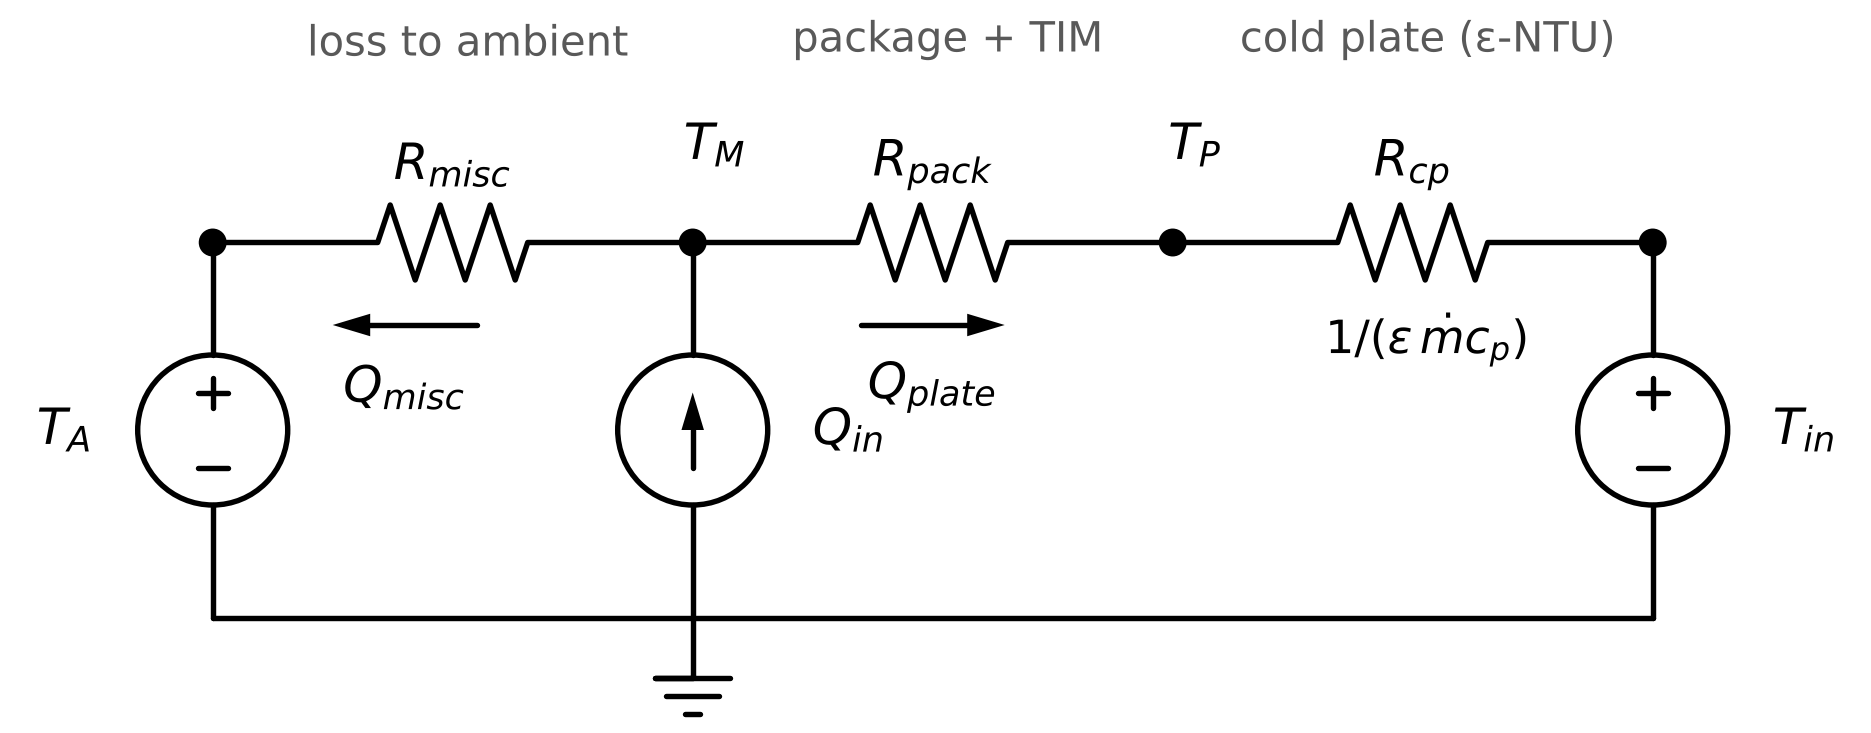
\includegraphics[width=0.85\linewidth]{thermal_network}
  \caption{Thermal network as an electrical analogue (temperature $\equiv$
    potential, heat flow $\equiv$ current); $T_{\mathrm{A}}$ and $\Tin$ are fixed
    boundary conditions.}
  \label{fig:thermal-network}
\end{figure}

\subsection{\texorpdfstring{$\varepsilon$--NTU}{epsilon-NTU} Analysis of the Cold Plate}
\label{sec:eps-ntu}

For this analysis, the plate is considered isothermal at $T_{\mathrm{P}}$, so
coolant entering at $\Tin$ approaches the plate temperature exponentially. An
energy balance on a tube element of perimeter $P$ gives~\cite{bergman_fundamentals_2017}
\begin{equation}
  \frac{T_{\mathrm{P}} - T_{\mathrm{f}}(x)}{T_{\mathrm{P}} - \Tin}
    = \exp\!\left(-\frac{hPx}{\mdot\,\cp}\right).
  \label{eq:temp-profile}
\end{equation}
At the outlet ($x = L$, $PL = A$), the exponent is defined as the number of
transfer units, $\NTU = hA/(\mdot\,\cp)$. This is the ratio of the
wall-to-coolant convective conductance to the heat-capacity rate of the coolant.
Each transfer unit reduces the remaining plate-to-coolant temperature difference
by a factor of $e$, so the coolant absorbs about \SI{63}{\percent} of the maximum
possible heat after one transfer unit~\cite{bergman_fundamentals_2017}. Defining
the effectiveness $\varepsilon$ as this fraction gives
\begin{equation}
  \Qplate = \varepsilon\,\mdot\,\cp\,(T_{\mathrm{P}} - \Tin), \qquad
  \varepsilon = 1 - e^{-\NTU}, \qquad
  \Rcp = \frac{1}{\varepsilon\,\mdot\,\cp},
  \label{eq:effectiveness}
\end{equation}
\begin{equation}
  T_{\mathrm{P}} = \Tin + \Qplate\Rcp, \qquad
  \Tout = \Tin + \frac{\Qplate}{\mdot\,\cp}.
  \label{eq:plate-outlet}
\end{equation}
This is the effectiveness relation for one flow stream against an isothermal
surface~\cite{bergman_fundamentals_2017}. Its limits show whether a coolant is
limited by convection at the wall or by its ability to transport heat
(caloric-limited), as summarised in \cref{tab:ntu-regimes}.

\begin{table}[htbp]
  \centering
  \caption{Limiting regimes of the $\varepsilon$--NTU relation for an isothermal
    plate.}
  \label{tab:ntu-regimes}
  \small
  \begin{tabular}{@{}lllll@{}}
    \toprule
    Regime & NTU & $\varepsilon$ & $\Rcp$ & Lever to reduce $\Rcp$ \\
    \midrule
    Convection-limited & $\ll 1$ & $\approx \NTU$ &
      $\approx 1/(hA) + 1/(2\mdot\,\cp)$ & Raise $hA$ (Nu, area) \\
    Transitional & $\approx 1$ & $1 - e^{-\NTU}$ &
      $1/(\varepsilon\,\mdot\,\cp)$ & Both \\
    Caloric-limited & $\gg 1$ ($\gtrsim 3$) & $\to 1$ &
      $\to 1/(\mdot\,\cp)$ & Raise $\mdot\,\cp$ (flow rate) \\
    \bottomrule
  \end{tabular}
\end{table}

The isothermal-plate assumption relies on in-plane heat spreading within the
\SI{15}{\milli\metre} 6063 aluminium base (\cref{fig:coldplate-heatflow}). The
assumption weakens as the coolant temperature rise between inlet and outlet,
$\Delta T_{\mathrm{cool}} = \Qplate/(\mdot\,\cp)$, increases. The predicted rise
is below \SI{2}{\celsius} for water but approximately
\SIrange{17}{20}{\celsius} for Galinstan, so the model is expected to describe
water better than Galinstan. For this reason, the package resistance $\Rpack$
was calibrated on the two turbulent water tests, which give the most nearly
isothermal plate, as \SI{0.242}{\celsius\per\watt}. It was then held at this
value for all flows and both coolants.

\begin{figure}[htbp]
  \centering
  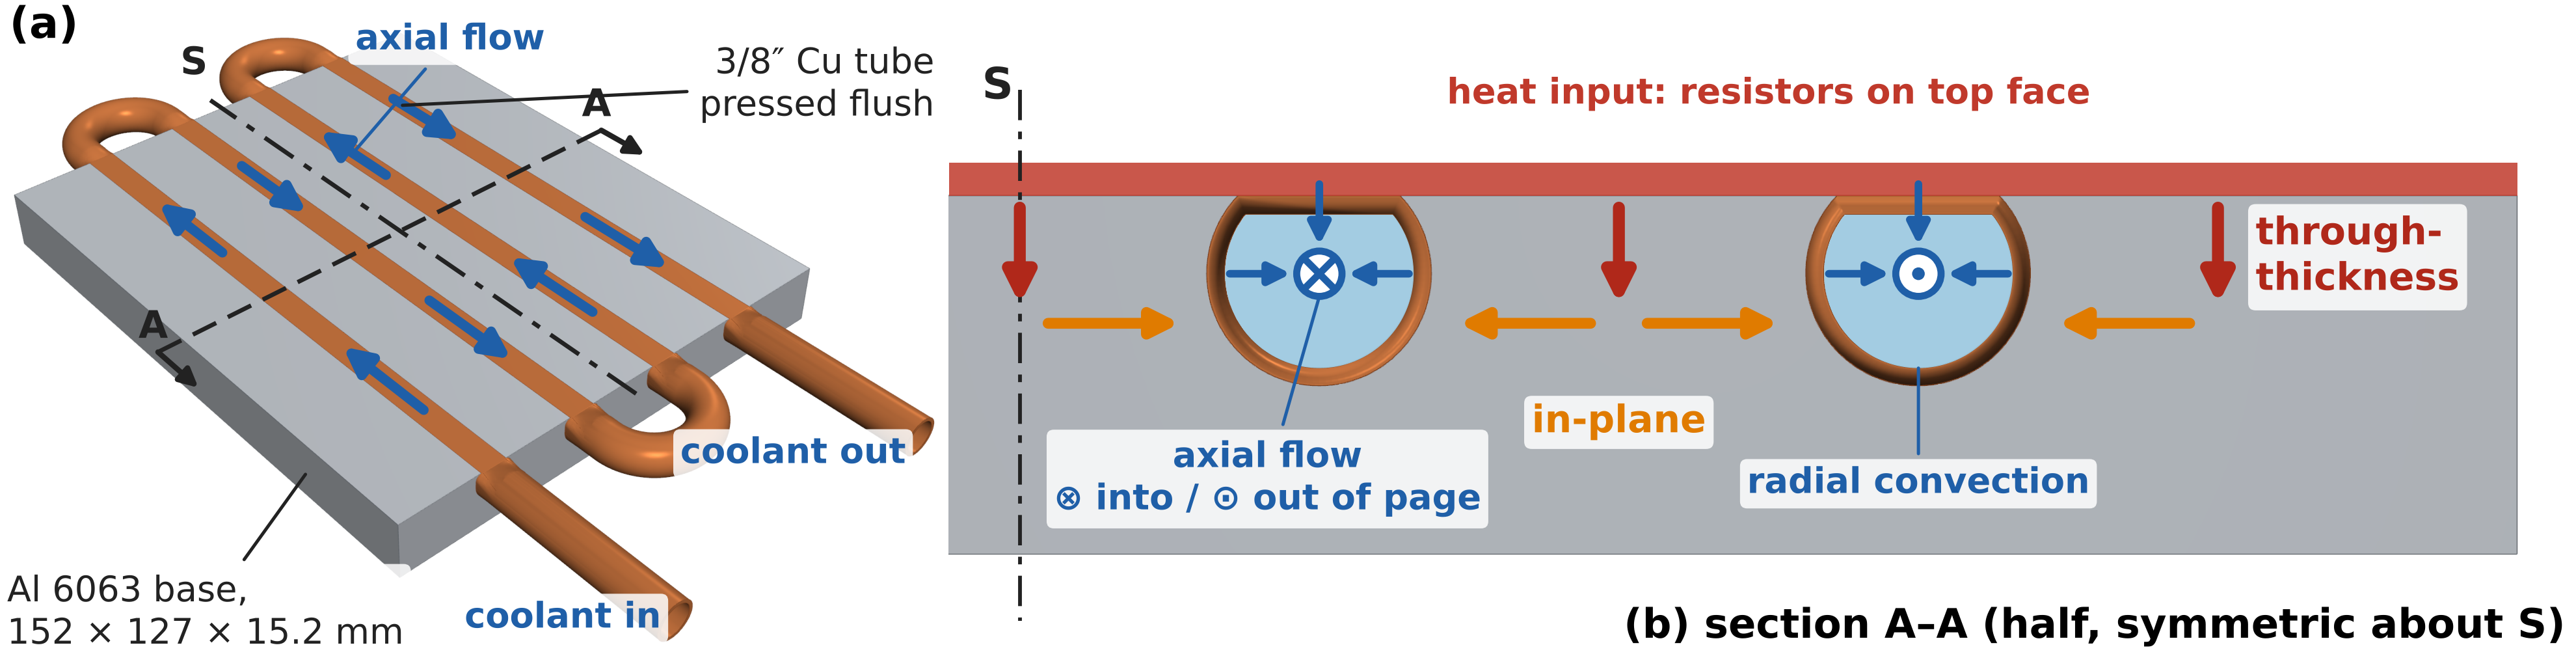
\includegraphics[width=0.85\linewidth]{coldplate_heat_flow}
  \caption{Heat-flow directions in the cold plate: in-plane spreading (plate),
    through-thickness conduction (part of $\Rpack$), axial flow and radial
    convection ($R_{\mathrm{conv}}$).}
  \label{fig:coldplate-heatflow}
\end{figure}

\subsection{Convection Correlations and Test Conditions}
\label{sec:convection}

The $\varepsilon$--NTU model requires an estimate of the heat transfer
coefficient $h$ between the tube wall and the coolant. It is obtained from
standard correlations for the Nusselt number, $\mathrm{Nu} = hD/k$, a
dimensionless measure of how effectively the flowing coolant removes heat from
the wall. For laminar flow, the Shah and London
correlation~\cite{shah_laminar_1978} gives the mean Nu along a tube at constant
wall temperature, including the thermal entry region where heat transfer is
highest. It is applied to each \SI{152}{\milli\metre} pass separately, on the
assumption that the U-bends mix the flow. For turbulent water
($\mathrm{Re} \geq 4000$), Gnielinski's correlation~\cite{bergman_fundamentals_2017}
is used, and no estimate is made in the transitional range
$2300 < \mathrm{Re} < 4000$. Galinstan remains laminar up to
\SI{5}{\milli\litre\per\second} ($\mathrm{Re} \leq 2110$). The correlations and
worked calculations for both coolants are given in \cref{app:convection}.

The NTU analysis uses these correlations for both coolants. For the turbulent
water tests, however, the cold-plate resistance given in the ATS-TCP-1001
datasheet~\cite{advanced_thermal_solutions_inc_tubed_2021} was later found to
fit the measured data better, so the temperature predictions for these tests
use the datasheet values, fitted as
$\Rcp = 0.0274\,\Vdot^{-0.415}$~\si{\kelvin\per\watt} ($\Vdot$ in
\si{\litre\per\minute}). The Galinstan and laminar water tests use the
$\varepsilon$--NTU model.
\Cref{tab:coolant-properties,tab:tests} summarise the cold-plate geometry, the
coolant properties and the test conditions.

\begin{table}[htbp]
  \centering
  \caption{Cold-plate geometry (ATS-TCP-1001) and coolant properties.}
  \label{tab:coolant-properties}
  \small
  \begin{tabularx}{\linewidth}{@{}>{\raggedright\arraybackslash}p{4.3cm}ll L@{}}
    \toprule
    Quantity & Galinstan & Water & Note \\
    \midrule
    Tube bore / heated length per pass & \SI{8}{\milli\metre} / \SI{152}{\milli\metre}
      & \SI{8}{\milli\metre} / \SI{152}{\milli\metre}
      & Bore measured; plate length and 4 passes
        from~\cite{advanced_thermal_solutions_inc_tubed_2021};
        $A = \SI{0.0153}{\metre\squared}$ \\
    $\rho$ (\si{\kilogram\per\metre\cubed}) / $\cp$ (\si{\joule\per\kilogram\per\kelvin})
      & 6370 / 366 & 1000 / 4182
      & Galinstan $\rho$~\cite{kwon_project_2025}, $\cp$~\cite{zhang_experimental_2019} \\
    $k$ (\si{\watt\per\metre\per\kelvin}) / $\mu$ (\si{\milli\pascal\second})
      & 16.5 / 2.4 & 0.60 / 1.0 & \cite{kwon_project_2025} \\
    \bottomrule
  \end{tabularx}
\end{table}

\begin{table}[htbp]
  \centering
  \caption{Steady-state tests, estimated coolant temperature rise and cold-plate
    resistance used in the predictions.}
  \label{tab:tests}
  \small
  \setlength{\tabcolsep}{4.5pt}
  \begin{tabular}{@{}llrrlrr@{}}
    \toprule
    Test & Flow & $\Qin$ (\si{\watt}) & Re & Regime &
      $\Delta T_\mathrm{cool}$ (\si{\celsius}) & $R_\mathrm{cp}$ (\si{\celsius\per\watt}) \\
    \midrule
    Galinstan, full (\SI{18}{\ampere}) & \SI{1.4}{\milli\litre\per\second}  & 72 & 591  & Laminar   & 17.8\textsuperscript{\textdagger} & 0.295 \\
    Galinstan, low (\SI{9}{\ampere})   & \SI{0.75}{\milli\litre\per\second} & 40 & 317  & Laminar   & 17.1\textsuperscript{\textdagger} & 0.555 \\
    Water & \SI{3.5}{\litre\per\minute}  & 72 & 9284 & Turbulent & 0.26 & 0.016\textsuperscript{\textdaggerdbl} \\
    Water & \SI{1.75}{\litre\per\minute} & 72 & 4642 & Turbulent & 0.52 & 0.022\textsuperscript{\textdaggerdbl} \\
    Water & \SI{0.73}{\litre\per\minute} & 72 & 1936 & Laminar   & 1.22 & 0.074 \\
    Water & \SI{0.5}{\litre\per\minute}  & 72 & 1326 & Laminar   & 1.78 & 0.088 \\
    \bottomrule
    \multicolumn{7}{@{}p{\linewidth}@{}}{\footnotesize
      $\Delta T_\mathrm{cool} = Q_\mathrm{plate}/(\mdot\,\cp)$, where
      $Q_\mathrm{plate}$ is $\Qin$ less the loss to ambient through
      $R_\mathrm{misc}$. $R_\mathrm{cp}$ is from the $\varepsilon$--NTU model
      unless marked.
      \textsuperscript{\textdagger}\,Galinstan $\mdot\,\cp$ estimated from the
      energy balance, so $\Delta T_\mathrm{cool}$ equals the measured
      $T_\mathrm{out} - T_\mathrm{in}$; nominal flows are from the EMF
      flow sensor.
      \textsuperscript{\textdaggerdbl}\,ATS datasheet
      fit~\cite{advanced_thermal_solutions_inc_tubed_2021};
      \SI{1.75}{\litre\per\minute} is slightly extrapolated below the lowest
      datasheet point (\SI{1.89}{\litre\per\minute}).}
  \end{tabular}
\end{table}
\edited{Turbulent water flows changed from 3.6 and \SI{1.8}{\litre\per\minute}
to the measured 3.5 and \SI{1.75}{\litre\per\minute} (58.3 and
\SI{29.2}{\milli\litre\per\second}) here and in later chapters. Re and
$\Delta T_{\mathrm{cool}}$ were recalculated; $\Rcp$, NTU, $\Rpack$ and the
predicted temperatures are unchanged at the precision shown (the datasheet
$\Rcp$ changes by \SI{0.0002}{\celsius\per\watt}). Thermal\_Network\_Model.xlsx
still uses 3.6 and \SI{1.8}{\litre\per\minute}.}

\subsection{Conjugate Heat Transfer Simulation}
\label{sec:cht}

The thermal network reproduces the measured resistor temperatures by lumping the
cold plate into a single isothermal node. This is reasonable for water, but for
Galinstan the plate is not isothermal. The network also cannot resolve how heat
spreads from the discrete resistor footprints through the press-fit tube
contact, nor capture flow redevelopment at the U-bends or the transitional flow
suspected in the low-flow water tests. A conjugate heat transfer (CHT)
simulation, which solves the coolant flow and the conduction through the solids
together, was therefore completed in SimScale~\cite{simscale_gmbh_simscale_2021}.
It resolves the temperature fields in the plate and coolant, and the local peak
temperatures that govern component and insulation limits.

To reduce computation time, a simplified model of the cold plate was first
created in Onshape~\cite{ptc_onshape_2015} and imported into SimScale
(\cref{fig:cfd_setup}). An internal flow volume was then defined in the
geometry. The solids were assigned SimScale's default material properties for
aluminium and copper, and water used the default material. A custom Galinstan
material was created from the properties in \cref{tab:coolant-properties}. The
simulation settings and boundary conditions are summarised in
\cref{tab:simulation-setup}, and parameters not listed were left at their
default values.

\begin{figure}[htbp]
    \centering
    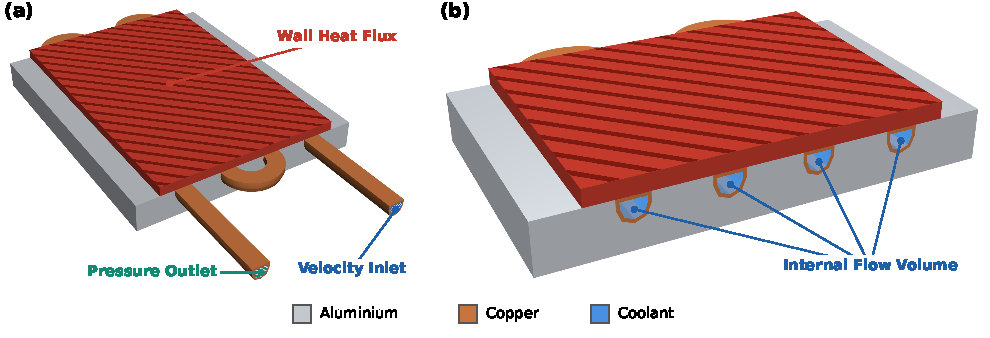
\includegraphics[width=\textwidth]{coldplate_figure.pdf}
    \caption{Cold-plate model used for the CHT analysis.
        (a)~Isometric view and (b)~cut showing the internal flow volume.}
    \label{fig:cfd_setup}
\end{figure}

The boundary conditions were chosen to match each test. The inlet was set as a
velocity inlet at the measured inlet temperature of the test (for example,
\SI{29.8}{\celsius} for the full-flow Galinstan test), with the velocity
adjusted to give the measured flow rate. The outlet was held at a pressure of
\SI{1}{atm}. The heat input was applied as a heat flux equal to the heat
reaching the cold plate, $\Qplate$, rather than the full electrical input,
because part of the input is lost to the environment
(\cref{sec:thermal-network}). For the full-flow Galinstan test this was about
\SI{60}{\watt} of the \SI{72}{\watt} input, and for the low-flow Galinstan test
about \SI{30}{\watt} of the \SI{40}{\watt} input, estimated from the measured
coolant temperature rise. The water run used the same $\Qplate$ as the water
tests, about \SI{62.6}{\watt}.

\begin{table}[htbp]
  \centering
  \caption{CHT simulation settings and boundary conditions.}
  \label{tab:simulation-setup}
  \small
  \begin{tabular}{@{}ll@{}}
    \toprule
    Parameter & Setting \\
    \midrule
    Analysis type    & Conjugate heat transfer \\
    Compressible     & Yes \\
    Flow model       & $k$--$\omega$ SST (turbulent); laminar for $\mathrm{Re} \leq 2110$ \\
    Time dependency  & Steady state \\
    Inlet            & Velocity inlet at the measured flow rate and inlet temperature \\
    Outlet           & Pressure outlet, \SI{1}{atm} \\
    Heat input       & Heat flux equal to $\Qplate$ of each test at the resistor footprints \\
    Mesh             & \num{427e3} cells (\cref{app:cht_validation}) \\
    \bottomrule
  \end{tabular}
\end{table}

Turbulent cases were solved with the $k$--$\omega$ SST turbulence model, and a
laminar model was used for the runs with an estimated $\mathrm{Re} \leq 2110$.
Mesh independence was therefore assessed separately for each flow regime and
each coolant. Each study was performed at the most demanding operating point,
the highest flow rate, where the boundary layers are thinnest, so that the
resulting mesh is conservative for all milder cases. Separate studies were
needed for the two coolants because Galinstan develops a thermal boundary layer
much thicker than its velocity boundary layer, whereas water has a thermal
boundary layer thinner than its velocity boundary layer and therefore requires
finer near-wall resolution for the temperature field. The same sequence of five
meshes, from \num{73e3} to \num{1.5e6} cells, was used in every study, and the
\num{427e3}-cell mesh was adopted. The mesh study, the iterative convergence and
the comparison with experiment are given in \cref{app:cht_validation}. In
addition to the runs that reproduce each test, the cold plate was simulated
with Galinstan at four flow rates between \SI{0.75}{\milli\litre\per\second}
and \SI{5}{\milli\litre\per\second}, to compare the simulated cold-plate
resistance with the $\varepsilon$--NTU model beyond the flows the rig could
reach (\cref{sec:rcp-calc}).

\subsection{Calculation of the Cold-Plate Resistance}
\label{sec:rcp-calc}

The cold-plate resistance $\Rcp$ cannot be measured directly, because the plate
temperature $T_\mathrm{P}$ is not measured. It is therefore inferred from the
resistor and inlet temperatures by removing the package resistance from the
total resistance of the network in \cref{eq:network}:
\begin{equation}
  \Rcp = \frac{\Tres - \Tin}{Q} - \Rpack,
  \label{eq:rcp-inferred}
\end{equation}
where $\Tres$ is the mean of the left and right resistor temperatures, $Q$ is
the heat passing into the coolant and $\Rpack = \SI{0.242}{\celsius\per\watt}$
is the package resistance calibrated on the turbulent water tests. The same
definition is applied to the experimental and simulated results, so that both
are compared with the model on an equal basis (\cref{fig:galinstan_rcp_cfd}).

\paragraph{Experimental values.} $Q$ is the heat reaching the plate,
$\Qplate$, obtained by subtracting the loss to ambient through $\Rmisc$ from the
electrical input, as in \cref{eq:network}. The flow rate is taken from a
combination of the EMF flow sensor and the energy balance,
$\Vdot = \Qplate / [\rho\cp(\Tout - \Tin)]$, which agreed closely for the tests
completed in this study.

\paragraph{Simulated values.} The conjugate heat transfer results are taken at
the final iteration of each run on the \num{427e3}-cell mesh. $Q$ is obtained
from the coolant energy balance at the simulated flow rate,
\begin{equation}
  Q = \rho\cp\Vdot\,(\Tout - \Tin),
\end{equation}
which gives \SIrange{57.4}{58.2}{\watt} for all four runs, and $\Tres$ is the
mean of the two resistor probe temperatures.

\paragraph{Model values.} The $\varepsilon$--NTU model gives
$\Rcp = 1/(\varepsilon\,\mdot\,\cp)$ with $\varepsilon = 1 - e^{-\NTU}$
(\cref{sec:eps-ntu}), using the Shah and London mean Nusselt number for laminar
flow (\cref{app:convection}). Because Galinstan has $\NTU > 10$ across this
range, the model is effectively the caloric limit, $\Rcp \approx 1/(\mdot\,\cp)$.
\edited{Changed from $\NTU > 30$: the model gives $\NTU \approx 35$ at
\SI{1.4}{\milli\litre\per\second} but about 10.7 at
\SI{5}{\milli\litre\per\second}, which is still caloric-limited.}

% ---------------------------------------------------------------------
\section{Experimental Procedure}
\label{sec:programme}

Two experiments were conducted to answer the two research questions.
Experiment~1 compares the thermal performance of the water and Galinstan loops
across a range of flow rates, and its data were used to build and validate the
thermal models of \cref{sec:thermal-model}. Experiment~2 demonstrates
Galinstan's ability to cool a power-dense inductor and quantifies the
additional eddy-current loss induced in the coolant by the inductor's magnetic
field. Temperatures throughout each loop were logged continuously for the
duration of every test.

\subsection{Experiment 1: Baseline Thermal Comparison}
\label{sec:exp1}

The first experiment establishes a baseline comparison of the two cooling loops
and was run on both using identical procedures. Before each test, the data
logger was started and the coolant was circulated at the target flow rate, set
by the pump current for Galinstan and by the pump duty cycle for water. The
resistors were then switched on at the test heat load. Each test continued
until the system reached steady state, taken as a change of less than
\SI{0.5}{\celsius} over 30 minutes. The thermocouple readings at the resistor,
the cold-plate inlet and the cold-plate outlet were then recorded, together with
the flow rate and the heat load. At shutdown, the resistors were switched off
before the pump was ramped down.

The planned tests are given in \cref{tab:flow-rates}. The full-flow tests
evaluate the maximum heat transfer of the current systems, and the low-flow
tests provide data to inform and validate the thermal models. The no-flow tests,
run at a reduced heat load of \SI{12}{\watt}, measure the heat leakage to the
environment and give $\Rmisc$ (\cref{sec:thermal-network}). Two further tests
at lower flow rates,
\SI{0.73}{\litre\per\minute} and \SI{0.5}{\litre\per\minute}, were later
conducted on the water loop, using the valve to reduce the flow below the
controllable range of the pump. These give laminar water data, in the same flow
regime as Galinstan. The low-flow Galinstan test was run at a reduced heat load
of \SI{40}{\watt}, so that the resistor and the pump housing stayed below the
\SI{70}{\celsius} limit set by the resin of the MHD pump~\cite{kwon_project_2025}.

\begin{table}[htbp]
  \centering
  \caption{Planned experimental flow rates.}
  \label{tab:flow-rates}
  \small
  \begin{tabularx}{\linewidth}{@{}lccL@{}}
    \toprule
    Test & Water & Galinstan & Goal \\
    \midrule
    Full flow & \SI{58.3}{\milli\litre\per\second} & \SI{1.4}{\milli\litre\per\second}
      & Evaluate the maximum heat transfer of the current systems \\
    Low flow  & \SI{29.2}{\milli\litre\per\second} & \SI{0.8}{\milli\litre\per\second}
      & Provide data to inform and validate the thermal models \\
    No flow   & \SI{0}{\milli\litre\per\second}    & \SI{0}{\milli\litre\per\second}
      & Assess heat leakage to the environment \\
    \bottomrule
  \end{tabularx}
\end{table}

\subsection{Experiment 2: Inductor Cooling and Eddy-Current Loss}
\label{sec:exp2}

The second experiment demonstrates the ability of Galinstan to cool a
power-dense inductor and assesses the interaction between its leakage field and
the electrically conductive coolant. The thermal test follows the procedure of
Experiment~1, except that the inductor replaces the resistors. The inductor was
driven at its rated current of \SI{12}{\ampere} rms by an inverter and the
resonant tuning network of \cref{sec:capacitor-tuning}, giving an estimated heat
load of \SI{42.76}{\watt} (\cref{sec:model-validation}). The Galinstan was
operated at full flow, and the inductor temperatures were recorded with the
thermal camera. Any change in flow when the inductor was energised was captured
by the flow sensor.

The eddy-current loss induced by the leakage field was measured separately with
an Agilent E4980A LCR meter at an excitation current of about \SI{5}{\milli\ampere},
by recording the AC resistance $R_{\mathrm{ac}}$ of the inductor winding in four
configurations: (i)~the inductor alone, (ii)~the inductor on the
empty cold plate, (iii)~the inductor on the cold plate filled with Galinstan, and
(iv)~the inductor on the cold plate with a PVC vial of Galinstan standing beside
it, as shown in \cref{fig:vial-setup}. Any conductor in the leakage field adds
to the series resistance seen at the winding, so the change in resistance
between two configurations isolates the loss of the conductor that was added.
The measurements were taken at the \SI{85}{\kilo\hertz} operating frequency.
Because Galinstan and the cold plate are linear and non-magnetic, the added loss
at any current is $\Delta R_{\mathrm{ac}} I_{\mathrm{rms}}^{2}$, so the change in
resistance is a direct measure of the eddy-current loss. Finally, with the cold
plate removed, the vial was moved progressively further away from the inductor,
from \SIrange{1}{5}{\centi\metre}, to show how the loss in the coolant falls
with distance.

\begin{figure}[htbp]
  \centering
  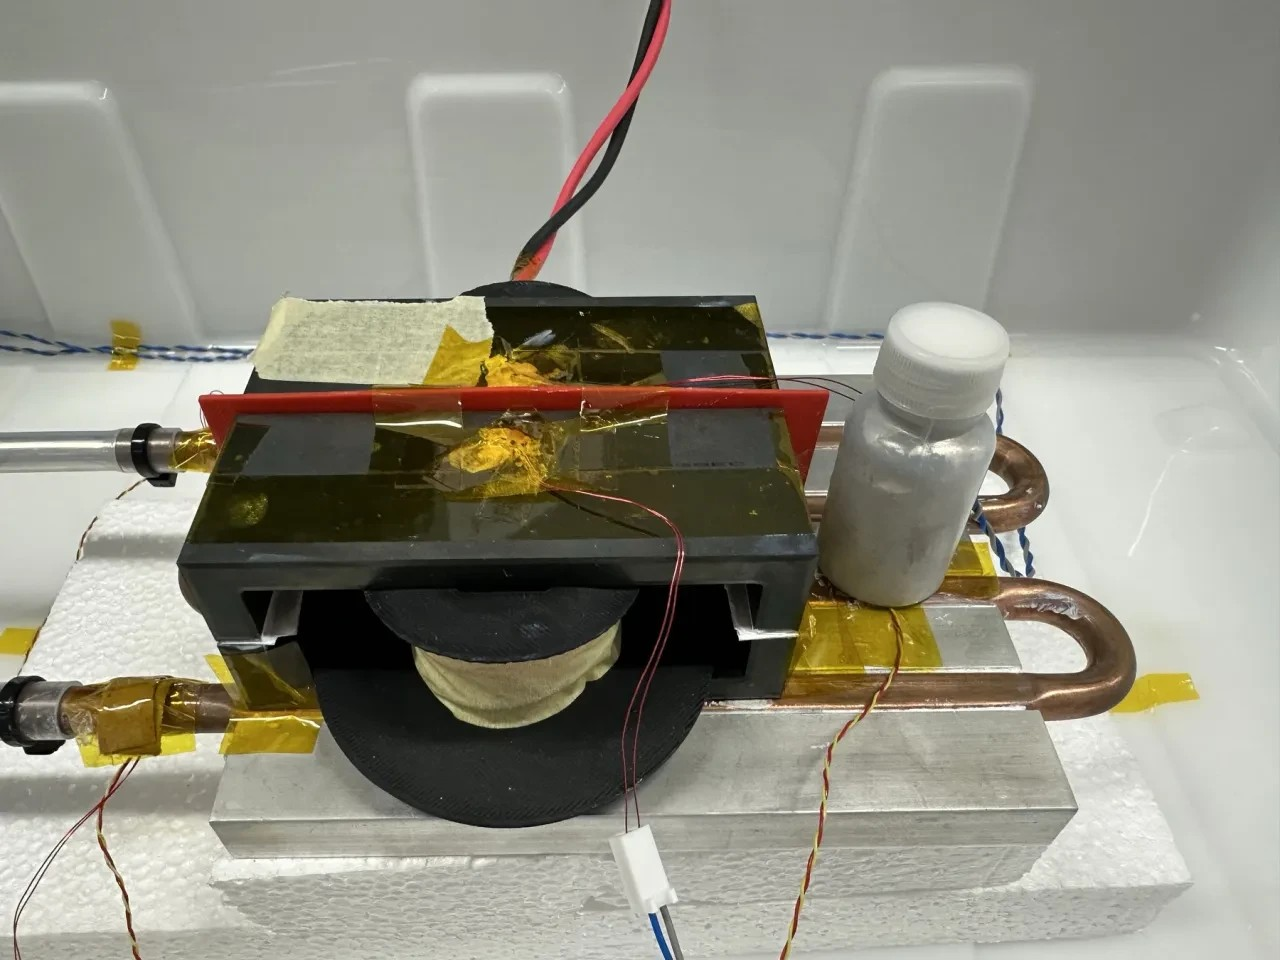
\includegraphics[width=0.6\linewidth]{inductor_vial_setup}
  \caption{Inductor on the Galinstan cold plate, with the PVC vial of Galinstan
    standing beside it, as used for configuration~(iv) of the eddy-current loss
    measurement.}
  \label{fig:vial-setup}
\end{figure}

% =====================================================================
%  Chapter 4 --   Results
% =====================================================================

\chapter{Results}
\label{ch:results}

\subsection{Analytical Thermal Models}

Table~\ref{tab:tn_results} compares the measured and predicted resistor
temperature $T_\mathrm{M}$ and coolant outlet temperature $T_\mathrm{out}$.
$R_\mathrm{pack}$ was calibrated on the two turbulent water tests, so those rows
check the method's consistency rather than validate it independently. Likewise,
Galinstan $T_\mathrm{out}$ is computed from the energy-balance flow rate and
agrees closely by construction. The independent test of the model is therefore
$T_\mathrm{M}$ in the Galinstan and laminar water tests.

\begin{table}[htbp]
    \centering
    \caption{Measured and predicted temperatures
        ($R_\mathrm{pack} = \SI{0.242}{\celsius\per\watt}$; turbulent water
        $R_\mathrm{cp}$ from the ATS datasheet, laminar water from the
        $\varepsilon$-NTU model). $\dagger$~Calibration tests. Galinstan
        $T_\mathrm{out}$ uses the energy-balance flow, so it agrees by construction.}
    \label{tab:tn_results}
    \begin{tabular}{lcccc}
        \toprule
        Test & \multicolumn{2}{c}{$T_\mathrm{M}$ (\si{\celsius})}
             & \multicolumn{2}{c}{$T_\mathrm{out}$ (\si{\celsius})} \\
        \cmidrule(lr){2-3}\cmidrule(lr){4-5}
             & Measured & Predicted & Measured & Predicted \\
        \midrule
        Galinstan \SI{1.4}{\milli\litre\per\second}               & 59.3 & 61.8 & 47.6 & 47.4 \\
        Galinstan \SI{0.75}{\milli\litre\per\second} (\SI{40}{\watt}) & 51.1 & 51.1 & 43.6 & 43.6 \\
        Water \SI{3.6}{\litre\per\minute}$^\dagger$               & 49.2 & 49.3 & 33.5 & 33.4 \\
        Water \SI{1.8}{\litre\per\minute}$^\dagger$               & 48.6 & 48.6 & 32.7 & 32.5 \\
        Water \SI{0.73}{\litre\per\minute}                        & 50.1 & 53.1 & 33.3 & 34.9 \\
        Water \SI{0.5}{\litre\per\minute}                         & 50.5 & 54.1 & 33.9 & 35.7 \\
        \bottomrule
    \end{tabular}
\end{table}

The predicted $T_\mathrm{M}$ lies within the $\pm\SI{3.1}{\celsius}$ measurement
band in five of the six tests, with an RMS error of \SI{1.8}{\celsius} for
Galinstan and \SI{2.3}{\celsius} for water. The turbulent water tests agree
within \SI{0.1}{\celsius}. The mid-flow Galinstan test
(\SI{1.0}{\milli\litre\per\second}) is excluded because its energy balance
closed at only about \SI{80}{\percent}, which indicates a flow-measurement error
or an incomplete approach to steady state.

The two laminar water tests are over-predicted by \SI{3.0}{\celsius} and
\SI{3.6}{\celsius}. In the laminar regime the model's $R_\mathrm{cp}$ rises to
\SIrange{0.074}{0.088}{\celsius\per\watt}, three to four times the turbulent
value. The measurements show no such loss: $T_\mathrm{M} - T_\mathrm{in}$ stays
between \SI{16.1}{\celsius} and \SI{16.6}{\celsius} from
\SIrange{3.6}{0.5}{\litre\per\minute}, and the measured $R_\mathrm{cp}$ follows
the manufacturer's turbulent trend (Figure~\ref{fig:flow_sweep}). This suggests
the flow in these tests was not fully laminar. The flow meter is uncertain below
\SI{1}{\litre\per\minute}, and the Reynolds number scales with
$\dot{V}/\mu$. With $\mu \approx \SI{0.75}{\milli\pascal\second}$ at the
\SI{33}{\celsius} test temperature, the \SI{0.73}{\litre\per\minute} test
reaches $\mathrm{Re} \approx 2600$, inside the transitional range, and any
under-reading of the flow would raise this further. Disturbances from the inlet
and U-bends can also persist at $\mathrm{Re} \approx$ 1300--1900, where the
development length of 66--97 tube diameters far exceeds the 19-diameter pass
length. If these tests are treated as turbulent, the datasheet trend predicts
$T_\mathrm{M}$ within \SI{0.7}{\celsius}. The laminar prediction is therefore
best read as a conservative upper bound. In the turbulent range the
$\varepsilon$-NTU model lies within \SI{15}{\percent} of the datasheet
(\SI{0.024}{\celsius\per\watt} against \SI{0.021}{\celsius\per\watt} at
\SI{2}{\litre\per\minute}).

Galinstan is caloric-limited at every tested flow: at least \SI{97}{\percent} of
its cold-plate resistance is $R_\mathrm{cal}$, so the pump, not the cold-plate
geometry, sets its thermal performance. Hodes et al.~\cite{hodes2014} reached
the same conclusion. Galinstan's volumetric heat capacity is 0.45 times that of
water, and caloric resistance made up \SI{55}{\percent} of the total for their
optimised Galinstan minichannel against \SI{40}{\percent} for water. The larger
share found here reflects a flow rate far below their optimum, and it means
higher pump flow, not improved convection, is the main route to better
liquid-metal performance in this system.
% =====================================================================
%  Chapter 5 -- Discussion
%  Structure follows Kwon (2025): interpretation of results, validity and
%  limitations, relevance to the field.
% =====================================================================
\chapter{Discussion}
\label{sec:discussion}

This chapter interprets the results of \cref{ch:results} against the two
research questions. The thermal performance and pumping power of the Galinstan
loop are discussed first (RQ1), followed by the inductor experiment (RQ2). The
validity and limitations of the measurements and models are then considered,
and finally the relevance of the findings to the cooling of PECs.

% ---------------------------------------------------------------------
\section{Interpretation of Results}
\label{sec:disc-interpretation}

\subsection{Thermal Performance of Galinstan in the Tested Cold Plate}
\label{sec:disc-performance}

The results in \cref{sec:results-measured} show that, at the flow rates
achieved, the Galinstan loop cooled the resistors less effectively than the
water loop, with a total thermal resistance 1.8 to 3.1 times higher
(\cref{tab:measured-performance}). However, the Galinstan tests ran at
\SIrange{0.8}{1.5}{\milli\litre\per\second}, one to two orders of magnitude below
the water tests (\SIrange{8.3}{58.3}{\milli\litre\per\second}). The comparison
therefore reflects the flow the MHD pump could deliver rather than a general
disadvantage of Galinstan as a coolant.

The reason lies in the limiting regime of the cold plate. Galinstan's NTU was 35
to 65 in the tests, so $\varepsilon \approx 1$ and $\Rcp \approx 1/(\mdot\,\cp)$.
The coolant therefore leaves the plate at almost the plate temperature, and heat
removal is limited by the ability of the flow to store and transport heat.
Galinstan's high thermal conductivity gives a wall heat transfer coefficient of
about \SI{7700}{\watt\per\metre\squared\per\kelvin}, roughly 7.5 times that of
laminar water (\cref{app:convection}). Its convective resistance $1/(hA)$ of
\SI{0.0085}{\celsius\per\watt} is lower than that of water even in turbulent
flow (\SIrange{0.012}{0.023}{\celsius\per\watt}). This advantage, however, is
not used in the current setup, because the convective term accounts for less
than \SI{3}{\percent} of Galinstan's $\Rcp$. Water, by contrast, has
$\NTU \approx 0.3$--0.4 at every tested flow, so convection makes up about
\SI{85}{\percent} of its $\Rcp$. These results support H1: Galinstan lowers the
convective resistance, but its low volumetric heat capacity and low flow rate
give a caloric resistance at least as large as the package resistance, so the
total resistance of the Galinstan loop is higher than that of the water loop.

\Cref{fig:disc-regimes}(a) extends this analysis over the full flow range.
Galinstan remains caloric-limited ($\NTU > 3$) over the whole laminar range and
up to about \SI{50}{\milli\litre\per\second}. Water, in contrast, stays close to
the convection-limited boundary above about \SI{10}{\milli\litre\per\second}.
For a caloric-limited coolant, the most important property is the volumetric
heat capacity $\rho\cp$, and here water has the advantage
(\cref{tab:disc-properties}): it absorbs about 1.8 times more heat per unit
volume per degree.

The same behaviour gives the Galinstan loop a much larger actuation range.
Because its cold plate is caloric-limited, its resistance follows the flow:
roughly halving the Galinstan flow, from 1.45 to
\SI{0.77}{\milli\litre\per\second}, raised the total resistance from 0.488 to
\SI{0.799}{\celsius\per\watt} (\cref{tab:measured-performance}). The
convection-limited water plate, in contrast, barely responded, with the total
resistance changing only from 0.257 to \SI{0.267}{\celsius\per\watt} over a
seven-fold change in flow. As discussed in \cref{sec:reliability}, the
flow rate of a single-phase loop is the control input used to suppress the
temperature swing of a component, part of the reliability requirement for PEC
thermal management (\cref{tab:cooling-strategies}). The pressure of an MHD pump
scales directly with its current (\cref{sec:em-pumping}), so the Galinstan loop
offers direct control over the component temperature through the pump current
across a wide range. In the tested water loop, changing the flow had almost no
effect on the resistor temperature. This range comes at the cost of a higher
resistance at the flows achieved here, but it is an advantage where the
temperature swing, rather than the peak temperature, limits component lifetime.

\begin{table}[htbp]
  \centering
  \caption{Coolant properties relevant to suitability. Thermal properties are
    those used in the model (\cref{tab:coolant-properties}).}
  \label{tab:disc-properties}
  \small
  \begin{tabularx}{\linewidth}{@{}lrrX@{}}
    \toprule
    Property & Galinstan & Water & Implication \\
    \midrule
    $\rho\cp$ (\si{\mega\joule\per\metre\cubed\per\kelvin})
      & 2.33 & 4.18 & Water carries 1.8$\times$ more heat per unit flow \\
    $k$ (\si{\watt\per\metre\per\kelvin}) & 16.5 & 0.60
      & Galinstan $h$ is about 27$\times$ higher at equal Nu \\
    $\mu$ (\si{\milli\pascal\second}) & 2.4 & 1.0
      & Laminar pressure drop 2.4$\times$ higher at equal flow \\
    $\rho$ (\si{\kilogram\per\metre\cubed}) & 6370 & 1000
      & 6.4$\times$ coolant mass for the same volume \\
    Pr & 0.053 & 6.97 & Heat diffuses far faster than momentum in Galinstan \\
    Electrical conductivity (\si{\siemens\per\metre})
      & $3.46 \times 10^{6}$~\cite{noauthor_gainsn_nodate} & $\ll 1$
      & Galinstan can be pumped electromagnetically, but heats and is retarded
        in AC fields \\
    Liquid range at \SI{1}{atm} (\si{\celsius})
      & 10 to $>1300$~\cite{noauthor_gainsn_nodate,hodes_potential_2014}
      & 0 to 100 & Galinstan cannot boil at component temperatures \\
    \bottomrule
  \end{tabularx}
\end{table}
\edited{\Cref{tab:disc-properties}: citations added for the electrical
conductivity and liquid range, matching \cref{tab:galinstan-properties}. The
lower end of the liquid range was $-19$; it is now \SI{10}{\celsius}, the
melting point of the grade used in this work (\cref{tab:galinstan-properties}).}

\begin{figure}[htbp]
  \centering
  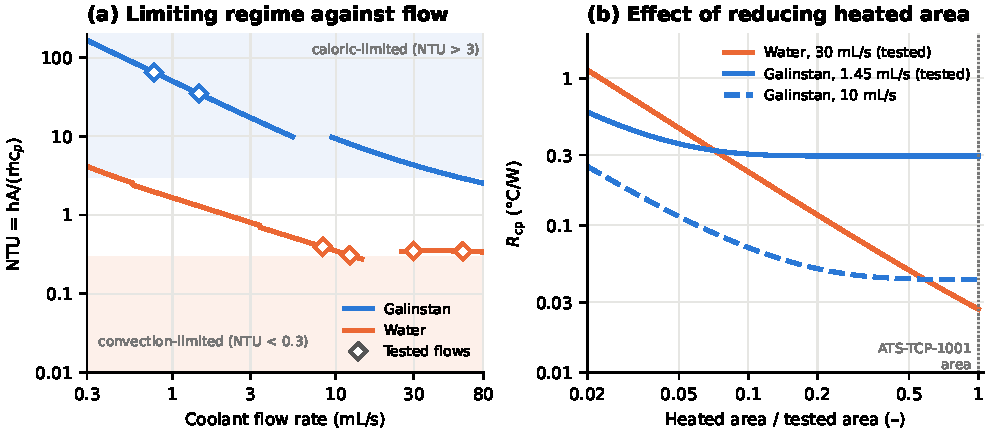
\includegraphics[width=\textwidth]{discussion_regimes.pdf}
  \caption{(a) NTU against flow rate for both coolants in the ATS-TCP-1001 cold
    plate, with the tested flows marked. Galinstan remains caloric-limited over
    the laminar range; water sits near the convection-limited boundary. Gaps
    mark the transitional range ($2300 < \mathrm{Re} < 4000$); turbulent
    Galinstan uses the Seban--Shimazaki correlation~\cite{bergman_fundamentals_2017}.
    (b) Indicative effect of reducing the heated area at fixed flow, with $h$
    held at its tested-geometry value. Water's $\Rcp$ rises in proportion to
    $1/A$, while Galinstan's at the tested flow is almost unaffected until the
    area falls to about a tenth of the tested value.}
  \label{fig:disc-regimes}
\end{figure}

\subsection{Pumping Power and Scalability}
\label{sec:disc-pumping}

RQ1 also asks how the pumping power of the two loops compares. At full flow, the
MHD pump drew \SI{0.85}{\watt}, about \SI{7}{\percent} of the \SI{11.5}{\watt}
drawn by the water pump, and it was more than 50 times smaller
(\cref{tab:pumps}). This is in line with An \emph{et al.}, who found that a
conduction pump drew less than \SI{15}{\percent} of the power of a mechanical
water pump for the same cooling performance~\cite{an_liquid_2024}, although here
the Galinstan loop also cooled less effectively. Per watt of pump power, the
Galinstan loop handled more heat, with a maximum coefficient of performance
(COP) of 200 against 47.6 for water. The low power draw does not, however,
reflect an efficient pump. The maximum mechanical efficiency of the MHD pump,
\SI{0.56}{\percent},
is an order of magnitude below the \SIrange{6}{10}{\percent} reported for DC
conduction pumps~\cite{an_liquid_2024,hodes_potential_2014}
(\cref{sec:em-pumping}), and far below the \SI{28.7}{\percent} of the
centrifugal water pump. Almost all of its input power is therefore dissipated
rather than delivered to the flow, which leaves considerable scope for a
redesigned pump. Fan \emph{et al.} show what is achievable: by reducing the
pressure drop of their loops to about one sixth with optimised connections and
cold plates, their MHD pumps reached flows of up to about
\SI{10}{\milli\litre\per\second} for less than
\SI{0.1}{\watt}~\cite{fan_liquid_2021,fan_high_2023} (\cref{tab:fan-comparison}). It is worth noting that the MHD pump was already at the
\SI{18}{\ampere} limit of its supply at full flow, so the Galinstan loop could
not be run at a higher flow.

For scalability, the more important question is the flow Galinstan would need
to match water. Because the cold plate is caloric-limited, the Galinstan $\Rcp$
is almost inversely proportional to the flow rate, as the simulations confirm up
to \SI{5}{\milli\litre\per\second} (\cref{fig:galinstan_rcp_cfd}). To match the
heat-capacity rate of
water at \SI{29.2}{\milli\litre\per\second} (\SI{122.0}{\watt\per\kelvin}),
Galinstan would need about \SI{52}{\milli\litre\per\second}, around 36 times the
full flow achieved here. The pressure of a DC conduction pump scales with current,
as shown by \cref{eq:mhd-pressure}, and the existing pump delivered
\SI{1.4}{\milli\litre\per\second} at the \SI{18}{\ampere} limit of its supply.
An increase in flow of this size would therefore require a redesigned pump
rather than simply a higher current. At equal volumetric flow, Galinstan also
needs about 2.4 times the pressure of water in laminar flow because of its higher
viscosity, and its density is 6.4 times that of water, which adds weight to the
loop (\cref{tab:disc-properties}). A comparison at equal pumping power, rather
than at the flow each pump could deliver, would therefore penalise Galinstan
further.

\subsection{Inductor Cooling and Eddy-Current Loss}
\label{sec:disc-inductor}

RQ2 asks whether the Galinstan loop can cool a power-dense inductor while adding
minimal loss, and how large the eddy-current loss induced in the coolant is. The
inductor was operated at an estimated loss of \SI{42.76}{\watt}, more than twice
the \SI{17.88}{\watt} datasheet loss limit above which its core requires active
cooling (\cref{sec:analytical-design}). Its maximum surface temperature was about
\SI{83}{\celsius} (\cref{fig:inductor-cam}), which shows that the Galinstan
loop can cool a power-dense inductor operating well beyond the loss its core
can dissipate without active cooling. The cooling effect of the plate is clear
from the steady-state thermal images: the upper core, which relies on natural
convection, ran markedly hotter than the lower core, which sits on the cold
plate (\cref{fig:inductor-cam-a}). This supports the first part of H2, that the
Galinstan loop cools the inductor beyond natural convection. The same difference
shows that the single-sided cold plate leaves part of the inductor's loss to be
removed by convection, and cooling both cores, as in the inductor of Gao
\emph{et al.}~\cite{gao_modeling_2022}, would make better use of the coolant.

The eddy-current measurements support the second part of H2. Placing the
inductor on the cold plate added \SI{11.7}{\milli\ohm} to the winding
resistance, whereas filling the plate with Galinstan added only
\SI{1.0}{\milli\ohm}, less than a tenth of the plate's own contribution. As
argued in H2,
the metal of the cold plate between the inductor and the
coolant is several skin depths thick at \SI{85}{\kilo\hertz}, so it shields the
Galinstan from the leakage field. Unshielded Galinstan is far more exposed: its
own skin depth at this frequency is about \SI{0.9}{\milli\metre} (for
$\sigma = \SI{3.46e6}{\siemens\per\metre}$~\cite{noauthor_gainsn_nodate}),
comparable to practical channel dimensions. The vial of Galinstan outside the
plate added \SI{10.3}{\milli\ohm}, an order of magnitude more than the coolant
inside the plate, although its volume and position differ. This agrees with the
initial ANSYS simulation, which found that \SI{1}{\milli\metre} of copper
shielding reduced the eddy-current loss in the coolant by more than
\SI{70}{\percent} (\cref{sec:inductor-design}). Without the plate, the effect of
the vial also fell with distance, from \SI{9.0}{\milli\ohm} at
\SI{1}{\centi\metre} to \SI{2.15}{\milli\ohm} beyond \SI{4}{\centi\metre}
(\cref{fig:rac_distance}), so keeping unshielded coolant a few centimetres from
the magnetics also limits the loss. Finally, the coolant flow did not change
measurably when the inductor was energised, which supports the final part of
H2.

% ---------------------------------------------------------------------
\section{Validity and Limitations}
\label{sec:disc-validity}

The steady-state data collected in this study are consistent across the two
loops and with the thermal models, but the conclusions rest on two Galinstan
tests and four water tests, and their limitations should be weighed. Four points
stand out.

First, the low-flow water results are limited by the flow measurement rather
than by the model. The measured $\Tres - \Tin$ stays between
\SI{16.1}{\celsius} and \SI{16.6}{\celsius} from
\SIrange{58.3}{8.3}{\milli\litre\per\second}, and the measured $\Rcp$ of
\SI{0.025}{\celsius\per\watt} at \SI{0.5}{\litre\per\minute} lies below water's
caloric limit $1/(\mdot\,\cp)$ of \SI{0.029}{\celsius\per\watt} at the indicated
flow (\cref{fig:water_rcp}). A cold plate cannot have $\Rcp < 1/(\mdot\,\cp)$, so
the true flow in that test must have been at least
\SI{9.6}{\milli\litre\per\second}, about \SI{15}{\percent} above the reading.
This supports the conclusion that the flow meter under-reads below its rated
range. It is also likely that these tests were not truly laminar. With the water
viscosity of about \SI{0.75}{\milli\pascal\second} at the \SI{33}{\celsius} test
temperature, the \SI{0.73}{\litre\per\minute} test reaches
$\mathrm{Re} \approx 2600$, in the transitional range, and any under-reading of
the flow raises this further. Disturbances from the pump, the valve and the
U-bends can also persist in the short passes, where the thermal entry length far
exceeds the pass length. If these tests are treated as turbulent, the datasheet
trend predicts $\Tres$ within \SI{0.7}{\celsius}, so the laminar
predictions in \cref{tab:tn_results} are best read as a conservative upper
bound.

Second, $\Rpack$ was calibrated on the turbulent water tests, where the plate is
close to isothermal. Galinstan's coolant temperature rise of
\SIrange{17}{18}{\celsius} violates this assumption: the outlet end of the plate
runs hotter than the mean, and the $\Rpack$ inferred for Galinstan ranges from
\SIrange{0.19}{0.24}{\celsius\per\watt} for an isothermal plate to
\SIrange{0.33}{0.51}{\celsius\per\watt} for uniform heat flux. The full-flow
Galinstan point lying slightly below its caloric limit (\cref{fig:galinstan_rcp})
is consistent with this. The Galinstan flow itself also relies on a small EMF,
which is less accurate at lower pump current, although it agreed with the energy
balance to within \SI{4}{\percent}. The lumped model therefore describes
Galinstan less reliably than water, although its prediction of the Galinstan
resistor temperatures to within \SI{2.5}{\celsius} (\cref{sec:results-tn})
shows that it captures the dominant behaviour.

Third, the conjugate heat transfer simulations address the main weakness of the
lumped model. They are mesh-independent above \num{427e3} cells and reproduce
all four probe temperatures within \SI{1.4}{\celsius} for both Galinstan tests.
The consistent over-prediction of the right-hand resistor by about
\SI{1.3}{\celsius} in both runs suggests a small systematic asymmetry in the
model, such as the heat-load distribution, rather than random error. For water,
the model under-predicts the resistor temperatures by about
\SIrange{2.3}{2.4}{\celsius}, which points to an over-predicted wall heat
transfer coefficient in the turbulent model (\cref{app:cht_validation}). The
model is therefore slightly pessimistic for Galinstan and optimistic for water,
so any advantage it shows for Galinstan is, if anything, understated. With this
in mind, the CHT model can be used with reasonable confidence to compare
geometries and flows that the test rig could not reach.

Fourth, the inductor experiment was run at a single operating point. Its heat
load is an estimate from the core-loss model and the measured winding
resistance, and the measured surface temperature of about \SI{83}{\celsius} is
above the \SI{65}{\celsius} assumed when the core loss was modelled, so the true
core loss will differ from the \SI{30.81}{\watt} estimate. The AC resistances
in \cref{fig:rac_configurations,fig:rac_distance} were measured at the
\SI{85}{\kilo\hertz} operating frequency, but each value comes from a single
measurement at low excitation, and the absolute resistance varied between
sessions, so only changes within a session are compared.

More generally, the study used a single cold plate designed for water, and the
coolants were compared at the flow each pump could deliver rather than at equal
pumping power. The water temperature rise across the plate was also below the
thermocouple accuracy, so the water energy balance could not be checked
independently.

% ---------------------------------------------------------------------
\section{Relevance to the Field}
\label{sec:disc-suitability}

The NTU analysis gives a clear criterion for where Galinstan is advantageous:
where the cooling surface, rather than the coolant flow, limits heat removal,
that is, where water would be convection-limited. \Cref{fig:disc-regimes}(b)
illustrates this using the $\varepsilon$--NTU model. The heated area is scaled
by a factor $f$ while the flow rate and heat transfer coefficient are held at
their values in the tested cold plate, so that $\NTU$ falls in proportion to $f$
and $\Rcp = 1/[\mdot\,\cp\,(1 - e^{-f\,\NTU_0})]$, where $\NTU_0$ is the value
for the full plate. This represents concentrating the same heat into a smaller
footprint or a shorter heated length, and the method and its assumptions are
given in \cref{app:area-scaling}. Reducing the heated area at fixed flow raises
water's $\Rcp$ almost in proportion, because water is already close to
convection-limited. At the tested flow, Galinstan's $\Rcp$ barely changes until
the area is reduced to about a tenth, because it simply uses up its excess
$hA$. At \SI{5}{\percent} of the tested area, Galinstan at
\SI{10}{\milli\litre\per\second} ($\Rcp \approx \SI{0.12}{\celsius\per\watt}$)
outperforms water at three times the flow
($\Rcp \approx \SI{0.46}{\celsius\per\watt}$). Galinstan's resistance only
begins to rise once $f\,\NTU_0$ falls to about 3, so a coolant that starts with a
large NTU can absorb a large reduction in area before its performance suffers.
Because $h$ is held fixed and pressure drop is not considered, the result is
indicative only, but it shows the type of application in which Galinstan's
conductivity becomes useful.
\edited{``About a fifth'' changed to ``about a tenth'': with $\NTU_0 = 34.9$ the
resistance starts to rise at $f \approx 3/\NTU_0 = 0.09$ (\cref{app:area-scaling}),
and \cref{tab:app-area} shows no change at $f = 0.2$. The caption of
\cref{fig:disc-regimes} was changed to match.}

Galinstan is therefore best suited to applications that combine (i)~high heat
flux over a small area, such as direct cooling of power semiconductors or local
hot spots, or minichannel and microchannel heat sinks; (ii)~a pump able to
deliver flow rates comparable to water, for which a sealed electromagnetic pump
with no moving parts may offer a reliability advantage; (iii)~component
temperatures near or above \SI{100}{\celsius}, where water would boil without
pressurisation; and (iv)~locations away from strong alternating magnetic fields,
or where the coolant is shielded from them by the cold plate, as in
\cref{sec:disc-inductor}.

In an IPT system, these criteria point to the power electronics, rather than the
pads, as the best place for Galinstan. In the \SI{10}{\kilo\watt} system of Kim
\emph{et al.}, the inverter and rectifier each dissipated about
\SIrange{70}{80}{\watt} in small switching devices placed away from the coupler,
where the heat flux is high and the magnetic field is weak
(\cref{sec:ipt-losses})~\cite{kim_thermal_2022}. The larger pad losses, by
contrast, are spread over about \SI{0.5}{\metre\squared} inside the strongest
alternating field at \SI{85}{\kilo\hertz}, so a cold plate under the pad would
see a low heat flux, for which water is adequate, together with a strong leakage
field. The inductor experiment shows that the leakage field need not rule
Galinstan out: coolant shielded by the metal of the cold plate added only
\SI{1.0}{\milli\ohm} to the winding resistance at \SI{85}{\kilo\hertz}, against
\SI{10.3}{\milli\ohm} for unshielded coolant beside the inductor
(\cref{sec:results-eddy}). Galinstan could therefore also cool compact
magnetics, such as the tank inductors and transformer, where heat is
concentrated in a small volume, provided the coolant is shielded.
\Cref{tab:disc-suitability} applies these criteria to the main components of an
IPT system.

\begin{table}[htbp]
  \centering
  \caption{Indicative suitability of Galinstan cooling for IPT system
    components, based on the criteria of \cref{sec:disc-suitability}.}
  \label{tab:disc-suitability}
  \small
  \begin{tabularx}{\linewidth}{@{}l>{\raggedright\arraybackslash}p{2.6cm}cX@{}}
    \toprule
    Component & Heat load character & Suitability & Reason \\
    \midrule
    Inverter and rectifier modules & High flux, small area & Good
      & Water likely convection-limited; much weaker AC fields than at the
        coupler \\
    Compact magnetics (tank inductors, transformer) & High flux, small volume
      & Possible
      & Leakage-field loss is small if the coolant is shielded by the cold
        plate (\cref{sec:results-eddy}) \\
    Coupler coils (Litz) and ferrite pads & Distributed, low flux & Limited
      & Large area, where water is adequate; strongest AC field, so the coolant
        must be shielded \\
    Resonant compensation capacitors & Moderate flux & Limited
      & Benefit only if close to their temperature limit; proximity to high
        voltage and AC fields \\
    Vehicle-side assembly & Weight-sensitive & Poor
      & 6.4$\times$ the coolant mass of water, and high material cost \\
    Large cold plates at low flow (as tested) & Low flux, large area & Poor
      & Caloric-limited; water carries 1.8$\times$ more heat per unit flow \\
    \bottomrule
  \end{tabularx}
\end{table}
\edited{\Cref{tab:disc-suitability}: coupler coils and pads changed from
``Poor'' to ``Limited'', since the eddy-current results show that a shielding
cold plate keeps the coolant's loss small, and a row added for compact magnetics,
which the inductor experiment represents.}

These findings agree with Hodes \emph{et al.}~\cite{hodes_potential_2014}, who
found that Galinstan's low volumetric heat capacity makes its caloric resistance
a larger share of the total than for water (\SI{55}{\percent} against
\SI{40}{\percent} in their optimised minichannel), and that its advantage depends
on geometries that exploit its high conductivity. The larger caloric share found
here (above \SI{97}{\percent}) reflects a cold plate designed for water and a
flow rate far below their optimum, rather than a contradiction of their result.
\issue{Check the volumetric heat-capacity ratio: Hodes quote 0.45, while the
properties used here give $2.33/4.18 = 0.56$; the difference is likely the
Galinstan $\cp$ (see the 360 vs \SI{366}{\joule\per\kilogram\per\kelvin} note).
\Cref{tab:galinstan-properties} also quotes 0.45.}

Despite the limitations above, the results show that a magnetohydrodynamically
pumped Galinstan loop can cool both a resistive load and a power-dense inductor,
and that the loss it adds near magnetics can be kept small when the coolant is
shielded by the cold plate. Its performance in the tested system is set by the
pump rather than by the coolant, so the case for liquid metal cooling in PECs
rests on higher-flow pumps and on cold plates designed to exploit its high
conductivity.

% ---------------------------------------------------------------------
\section{Recommendations for Further Work}
\label{sec:disc-limitations}

Further work should:
\begin{enumerate}
  \item compare the coolants at equal pumping power, using the CHT model to
    obtain the pressure drop as well as the temperature;
  \item test Galinstan at higher flow rates, closer to
    \SIrange{10}{30}{\milli\litre\per\second}, with an independently calibrated
    flow meter, which will require a redesigned pump;
  \item use the CHT model to evaluate small-area, high-flux geometries such as
    minichannel cold plates, where \cref{fig:disc-regimes}(b) indicates that
    Galinstan may outperform water;
  \item repeat the inductor test with the pump off and with the coolant
    unshielded, repeat the $R_{\mathrm{ac}}$ measurements to estimate their
    spread, and quantify eddy-current heating and MHD drag through coupled
    electromagnetic--thermal analysis before Galinstan is placed near an IPT
    coupler; and
  \item assess long-term material compatibility, since gallium alloys attack
    aluminium and copper requires protection at higher
    temperatures~\cite{an_liquid_2024}.
\end{enumerate}

% =====================================================================
%  Chapter 6 -- Conclusion
% =====================================================================
\chapter{Conclusion}
\label{ch:conclusion}

As PECs become more power-dense, removing their losses from a smaller volume
increasingly limits their design. This project evaluated MHD-pumped Galinstan as
a coolant for such converters, and identified where in an IPT system it is most
useful. A Galinstan loop and a water loop were compared on the same commercial
cold plate under resistive heat loads, the results were interpreted with an
$\varepsilon$--NTU thermal network and extended with a validated conjugate heat
transfer simulation, and the Galinstan loop was used to cool a power-dense
\SI{85}{\kilo\hertz} planar inductor.

\textbf{RQ1.} At the flows each pump could deliver, water outperformed
Galinstan, with a total resistance from the resistor to the coolant inlet of
\SIrange{0.257}{0.267}{\celsius\per\watt} against
\SIrange{0.488}{0.799}{\celsius\per\watt}. The $\varepsilon$--NTU analysis
explains this result and supports H1. Galinstan's high thermal conductivity
reduced its convective resistance to less than \SI{3}{\percent} of the cold-plate
resistance, but at \SIrange{0.77}{1.45}{\milli\litre\per\second} the plate was
caloric-limited, so Galinstan's low volumetric heat capacity set its
performance. The water plate, in contrast, was convection-limited and barely
responded to a seven-fold change in flow. The MHD pump drew only
\SI{0.85}{\watt}, against \SI{11.5}{\watt} for the water pump, giving a maximum
COP of 200 against 47.6, but its mechanical efficiency was only
\SI{0.56}{\percent}. The simulation shows that at
\SI{5}{\milli\litre\per\second}, the limit of laminar flow, the Galinstan total
resistance would fall to about \SI{0.29}{\celsius\per\watt}, within
\SI{14}{\percent} of water at a lower flow than any of the water tests.

\textbf{RQ2.} The Galinstan loop cooled the inductor, running at more than twice
the loss its core can dissipate without active cooling, to a maximum surface
temperature of about \SI{83}{\celsius}. Galinstan inside the cold plate added
only \SI{1.0}{\milli\ohm} to the winding AC resistance at
\SI{85}{\kilo\hertz}, against \SI{11.7}{\milli\ohm} for the plate itself and
\SI{10.3}{\milli\ohm} for unshielded Galinstan beside the inductor. The metal of
the cold plate therefore shields the coolant from the leakage field, supporting
H2, although the effect of the field on the flow could not be confirmed.

The main contribution of this work is to show when Galinstan is worth using.
Its advantage lies not in its conductivity alone, but in applications where the
heated area is small and the heat flux high: at \SI{5}{\milli\litre\per\second},
the model predicts that it outperforms water once the heated area falls below
about \SI{40}{\centi\metre\squared}. In an IPT system, this points to the
inverter and rectifier modules and to shielded compact magnetics, rather than
the large, distributed losses of the pads. These conclusions rest on a small
number of tests on a single cold plate designed for water, and the area
analysis is indicative only. Realising Galinstan's advantage will require a more
efficient, higher-flow pump with integrated power electronics, and a smaller cold
plate designed for liquid metal (\cref{sec:disc-further-work}).


%\backmatter
%\printbibliography[heading=bibintoc,title={References}]

%\appendix
% cleveref does not detect \appendix here, so appendix chapters were cited as
% "Chapter A". Label them (and their sections) as appendices explicitly; the
% names are set with the other \crefname commands in the preamble.
%\crefalias{chapter}{appendix}
%\crefalias{section}{subappendix}
%% =====================================================================
% Appendix: Validation of the SimScale conjugate heat transfer model
% Requires: graphicx, subcaption, siunitx (v2 \SI syntax, as in main report)
% =====================================================================

\chapter{Conjugate Heat Transfer Model}
\label{app:cht_validation}

The SimScale conjugate heat transfer (CHT) model was checked in three stages
before its results were used: a mesh independence study to bound the
discretisation error, a check of iterative convergence, and a comparison of the
converged probe temperatures against the experimental measurements. The
acceptance criterion throughout was the $\pm\SI{2.2}{\celsius}$ tolerance of the
thermocouples. Numerical errors well inside this band can be neglected, so any
remaining disagreement with experiment can be attributed to the modelling
assumptions or to the measurements themselves.

\subsubsection{Flow Regime and Mesh Independence}

Turbulent cases were solved with the $k$--$\omega$ SST turbulence model, and a
laminar model was used for runs with an estimated $\mathrm{Re} \leq 2110$.
Because the two models resolve the near-wall region differently, mesh
independence was assessed separately for each flow regime and each coolant.
Each study was performed at the most demanding operating point in its regime,
the highest flow rate, where the boundary layers are thinnest and the near-wall
gradients steepest. A mesh that resolves this case is therefore conservative for
the lower flow rates in the same regime. Separate studies were needed for the
two coolants because their Prandtl numbers differ by more than two orders of
magnitude. Galinstan ($\mathrm{Pr} \sim 10^{-2}$) develops a thermal boundary
layer much thicker than its velocity boundary layer, whereas water
($\mathrm{Pr} \approx 5$--$7$) has a thermal boundary layer thinner than its
velocity boundary layer and so needs finer near-wall resolution to capture the
temperature field. The same sequence of five meshes, from \num{73e3} to
\num{1.5e6} cells, was used in every study.
% NOTE: your earlier paragraph said "three" meshes; the figure shows five.

Figure~\ref{fig:mesh_independence} shows the study for Galinstan at
\SI{1.4}{\milli\litre\per\second}. The inlet and outlet temperatures vary by
less than \SI{0.1}{\celsius} across the full range. The inlet is fixed by the
boundary condition and the outlet is set largely by the bulk energy balance, so
neither depends strongly on near-wall resolution. The resistor temperatures are
the sensitive quantities, because they depend on resolving conduction through
the cold plate and the temperature gradient at the wall. The two coarsest
meshes underpredict them by up to \SI{2.75}{\celsius} relative to the finest
mesh, which exceeds the thermocouple tolerance. From \num{427e3} cells upward,
every probe lies within \SI{0.25}{\celsius} of the \num{1.5e6}-cell result.
Convergence is not strictly monotonic: the \num{427e3}- and \num{655e3}-cell
meshes slightly overshoot the finest mesh, and the refinement ratio between
successive meshes is not constant. Richardson extrapolation and the grid
convergence index, which assume monotonic convergence at a fixed refinement
ratio, were therefore not applied. Instead, the \SI{0.25}{\celsius} residual
change was compared directly with the measurement tolerance, and it is about
one ninth of that tolerance. The \num{427e3}-cell mesh was adopted for the
Galinstan simulations because it is the coarsest mesh whose discretisation
error is negligible against the measurement uncertainty.
% CHECK: confirm 427k is the mesh actually used for the reported runs.

\begin{figure}[htbp]
    \centering
    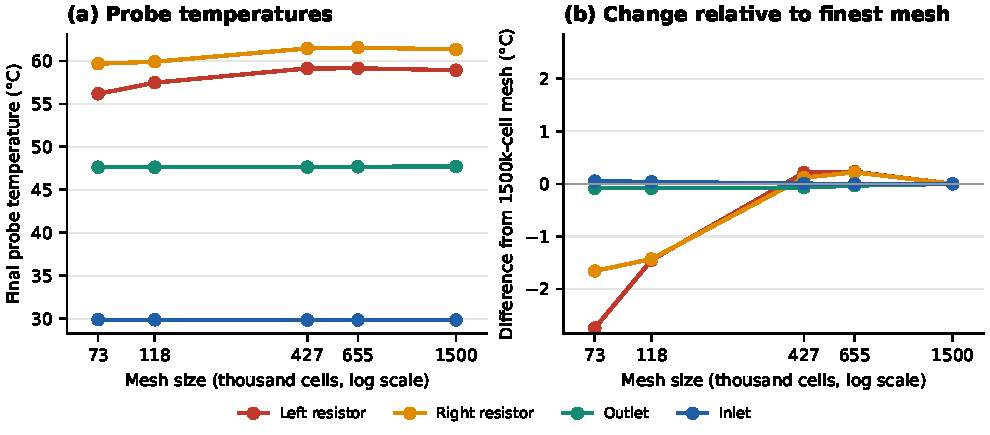
\includegraphics[width=\textwidth]{mesh_independence.pdf}
    \caption{Mesh independence study for Galinstan at
        \SI{1.4}{\milli\litre\per\second}: (a) final probe temperatures and
        (b) change relative to the \num{1.5e6}-cell mesh. All probes change by
        less than \SI{0.25}{\celsius} between \num{427e3} and
        \num{1.5e6} cells.}
    \label{fig:mesh_independence}
\end{figure}

Figure~\ref{fig:mesh_independence_water} shows the corresponding study for
the turbulent water model at \SI{3.6}{\litre\per\minute}. The pattern is the
same: the inlet and outlet vary by less than \SI{0.03}{\celsius}, and the
resistor temperatures are underpredicted on the coarsest meshes, by up to
\SI{2.5}{\celsius} at \num{73e3} cells. The fine meshes settle more slowly than
they do for Galinstan, however. At \num{427e3} cells the resistors still differ
from the \num{1.5e6}-cell result by up to \SI{0.58}{\celsius}, and at
\num{655e3} cells by \SI{0.38}{\celsius}, compared with less than
\SI{0.25}{\celsius} for Galinstan on the same meshes. This is the behaviour the
Prandtl number argument predicts: the thinner thermal boundary layer in water
needs finer near-wall resolution before the wall temperature gradient, and
hence the resistor temperature, stops changing. Above \num{427e3} cells the
resistor temperatures fall monotonically with refinement, so the
\num{1.5e6}-cell result is itself probably still a few tenths of a degree from a
fully mesh-independent value. The \num{427e3}-cell mesh was retained for water.
Its discretisation error of about \SI{0.6}{\celsius} is roughly a quarter of the
thermocouple tolerance: acceptable for comparison with experiment, but not
negligible in the way it is for Galinstan.
% CHECK: confirm which mesh the water runs used. If 655k, replace the last two
% sentences: error about 0.4 C, roughly a sixth of the tolerance.
% NOTE: this is the turbulent water study. If a laminar water study (low flow)
% was also run, it needs its own figure or a sentence here.

\begin{figure}[htbp]
    \centering
    \figureorplaceholder[width=\textwidth]{mesh_independence_water.pdf}
    \caption{Mesh independence study for water at
        \SI{3.6}{\litre\per\minute} ($k$--$\omega$ SST): (a) final probe
        temperatures and (b) change relative to the \num{1.5e6}-cell mesh,
        plotted on the same scale as Figure~\ref{fig:mesh_independence}. The
        inlet and outlet differ by only \SI{0.26}{\celsius} and overlap in (a).
        The resistor temperatures change by up to \SI{0.58}{\celsius} between
        \num{427e3} and \num{1.5e6} cells.}
    \label{fig:mesh_independence_water}
\end{figure}
\issue{The measured full water flow is now \SI{3.5}{\litre\per\minute}
(\SI{58.3}{\milli\litre\per\second}) in the main text. This appendix still says
the water simulations ran at \SI{3.6}{\litre\per\minute}. If that is the flow
set in SimScale, keep it and say so; otherwise change it to
\SI{3.5}{\litre\per\minute}.}

\subsubsection{Iterative Convergence}

The model was solved as a steady-state problem, and convergence was judged by
monitoring the probe temperatures, since these are the quantities compared
against experiment (Figure~\ref{fig:simscale_full}). The inlet temperature
settles within about 150 iterations because it is fixed by the boundary
condition. The outlet and resistor temperatures relax far more slowly, decaying
over several thousand iterations after an initial overshoot. This behaviour is
typical of conjugate heat transfer: heat crosses the solid regions by
conduction alone, so the solid temperature field relaxes much more slowly than
the flow field. By 4000 iterations the outlet temperature had levelled off,
while the resistor temperatures were still falling by about \SI{0.3}{\celsius}
over the final 1000 iterations.
% CHECK: drift read from the plot; confirm from the exported probe data.
The fully converged resistor temperatures would therefore be slightly lower
than those reported. This drift is small relative to the measurement tolerance,
but it is not zero, and its direction matters for the comparison below: it would
move the right resistor towards the measured value and the left resistor
slightly further below it. The water model converges much faster
(Figure~\ref{fig:simscale_water}). After an initial transient, every probe is
within \SI{0.01}{\celsius} of its final value by about 1000 iterations, and at
every mesh density no probe changes by more than \SI{0.001}{\celsius} over the
final 1000 iterations. Iterative error is therefore negligible for water.

\begin{figure}[htbp]
    \centering
    \begin{subfigure}{\textwidth}
        \centering
        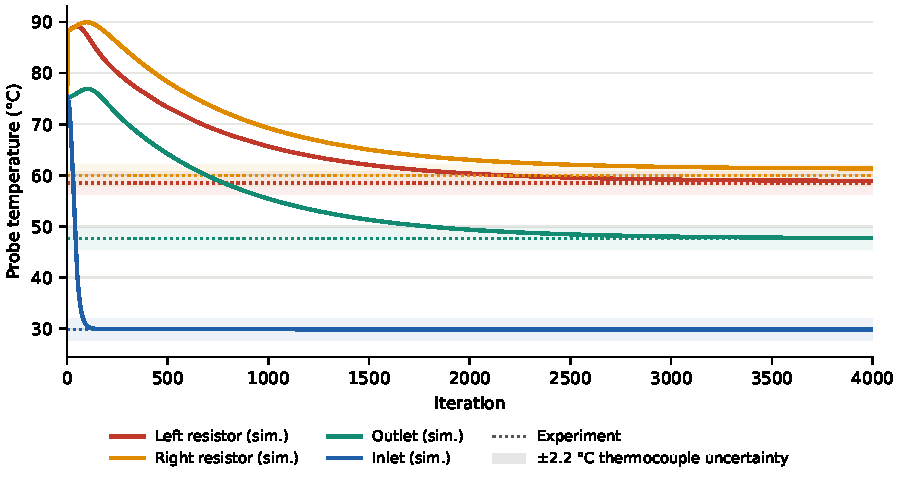
\includegraphics[width=0.9\textwidth]{simscale_convergence_full.pdf}
        \caption{Galinstan, \SI{1.4}{\milli\litre\per\second} (\SI{72}{\watt})}
        \label{fig:simscale_full}
    \end{subfigure}

    \vspace{0.6em}
    \begin{subfigure}{\textwidth}
        \centering
        \figureorplaceholder[width=0.9\textwidth]{simscale_convergence_water.pdf}
        \caption{Water, \SI{3.6}{\litre\per\minute} (\SI{72}{\watt}),
            \num{427e3} cells}
        \label{fig:simscale_water}
    \end{subfigure}
    \caption{Convergence of the SimScale conjugate heat transfer model against
        experiment. Solid lines show the simulated probe temperatures at each
        iteration; dotted lines show the measured values, with shaded bands for
        the $\pm\SI{2.2}{\celsius}$ thermocouple uncertainty. The measured
        resistor value is the mean of the two resistors. For Galinstan all
        probes lie within the measurement uncertainty at the final iteration;
        for water the resistors converge about \SI{2.4}{\celsius} below the
        measured value, just outside it.}
    \label{fig:simscale_convergence_both}
\end{figure}

\subsubsection{Comparison with Experiment}

For Galinstan, all four probes lie within the thermocouple tolerance of the
measured values at the final iteration (Figure~\ref{fig:simscale_full}). The inlet and outlet
agree to within about \SI{0.2}{\celsius}. The inlet agreement confirms that
the boundary condition was set correctly, rather than validating the model, and
the outlet agreement mainly confirms that the heat input and flow rate are
consistent with the energy balance. The resistor temperatures are the stronger
test, because they depend on the conduction path through the package and cold
plate and on the wall heat transfer coefficient the model predicts. The left
resistor is underpredicted by about \SI{0.5}{\celsius} and the right resistor
overpredicted by about \SI{1.4}{\celsius}. The model also predicts the right
resistor to be roughly \SI{2}{\celsius} warmer than the left, whereas the
measured temperatures are almost identical. This asymmetry lies within the
combined uncertainty, so the present instrumentation can neither confirm nor
rule it out.
\issue{The full-flow Galinstan data (\cref{fig:galinstan_transient}a) show the
right resistor at about \SI{60.1}{\celsius} and the left at about
\SI{58.6}{\celsius}, so the measured asymmetry is about \SI{1.5}{\celsius}, not
``almost identical''. The model's \SI{2}{\celsius} asymmetry is then close to
the measured one; reword this paragraph to match.}

The water model agrees less well (Figure~\ref{fig:simscale_water}). The
simulated inlet and outlet lie within \SI{0.15}{\celsius} of the measurements,
but this says little: the measured outlet rise is only \SI{0.4}{\celsius},
far below the sensor tolerance, so for water the outlet provides no useful
validation constraint. The resistors converge to \SI{46.9}{\celsius} and
\SI{46.8}{\celsius} against a measured mean of \SI{49.2}{\celsius}. They are
underpredicted by \SI{2.3}{\celsius} and \SI{2.4}{\celsius}, just outside the
tolerance band, and the resistor rise above the inlet is underpredicted by
about \SI{15}{\percent}. This gap is not a discretisation error. Refining the
mesh lowers the resistor temperatures further
(Figure~\ref{fig:mesh_independence_water}), so on the \num{1.5e6}-cell mesh the
underprediction grows to about \SI{2.9}{\celsius}. The discrepancy therefore
lies in the model itself. The cold plate, resistor package and their contact
are modelled identically for both coolants, and the Galinstan case shows no
comparable underprediction, which points towards the coolant side. The most
likely source is that the turbulent model overpredicts the wall heat transfer
coefficient for water. An error in the solid-side contact resistances that
happens to be masked in the Galinstan case cannot be excluded with only one
operating point per coolant.
% NOTE: measured values from Model Validation.xlsx ('FEM Model' sheet, water
% full flow): inlet 33.1, outlet 33.5, resistors 49.22 (mean). The raw log
% (CSV 17, 120-140 min) gives L 48.80, R 49.64 individually.

These results have clear limits. For Galinstan, agreement within
$\pm\SI{2.2}{\celsius}$ shows that the model is consistent with experiment at
the resolution of the measurements; it does not show that the model is
accurate to better than this. For water, the model is systematically optimistic,
predicting resistor temperatures about \SI{2}{\celsius} to \SI{3}{\celsius} too
low. The comparison also covers only one flow rate per coolant, so accuracy at
other operating points rests on the mesh study and the physical basis of the
model rather than on direct measurement. The model was therefore used where
these limits matter least: conclusions from the parametric studies are drawn
from trends and relative differences between configurations solved with the
same mesh and settings, which are less sensitive to systematic error than
absolute temperatures. The direction of the water bias also matters for the
coolant comparison. On average the model is slightly pessimistic for Galinstan and
optimistic for water, so any advantage the simulations show for Galinstan over
water is, if anything, understated.
% CHECK: confirm this matches how SimScale results are used in the main body.
%% =====================================================================
% Appendix: Convective heat transfer calculations for the thermal network
% Uses the report's macros: \Rcp, \Qplate, \Tin, \Tout, \mdot, \cp, \NTU, \Vdot
% Requires: amsmath, siunitx, booktabs, cleveref
% =====================================================================
\chapter{Convective Heat Transfer Calculations}
\label{app:convection}

This appendix explains how the cold-plate resistance $\Rcp$ in
\cref{sec:eps-ntu} is calculated from the flow rate and coolant properties, and
works through three of the tests in full.

\section{Heat Transfer Coefficient and Nusselt Number}

Heat passes from the tube wall into the coolant by convection, at a rate
\begin{equation}
  Q = hA\,(T_{\mathrm{wall}} - T_{\mathrm{f}}),
\end{equation}
where $A$ is the wetted area and $h$ the heat transfer coefficient
(\si{\watt\per\metre\squared\per\kelvin}). $h$ is not a material property; it
depends on the coolant, the flow and the geometry. Correlations therefore give
it in dimensionless form, as the Nusselt number
\begin{equation}
  \mathrm{Nu} = \frac{hD}{k}
  \qquad\Longrightarrow\qquad
  h = \frac{\mathrm{Nu}\,k}{D},
  \label{eq:app-nu}
\end{equation}
where $D$ is the tube bore and $k$ the coolant thermal conductivity. Nu is the
ratio of the heat actually removed by the flowing coolant to the heat that would
be conducted through a stationary layer of coolant of thickness $D$. Two
consequences matter here. First, for a given Nu, $h$ is proportional to $k$, so
Galinstan ($k = \SI{16.5}{\watt\per\metre\per\kelvin}$) gives roughly 27 times
the $h$ of water ($k = \SI{0.60}{\watt\per\metre\per\kelvin}$) at the same Nu.
Second, Nu depends on the flow regime and on how far along the tube the flow
has travelled, as described below.

\section{Flow Parameters}

Three dimensionless groups describe the flow:
\begin{align}
  \mathrm{Re} &= \frac{\rho u D}{\mu} = \frac{4\rho\Vdot}{\pi D \mu},
  & \mathrm{Pr} &= \frac{\mu\,\cp}{k},
  & \mathrm{Pe} &= \mathrm{Re}\,\mathrm{Pr},
  \label{eq:app-groups}
\end{align}
where $u$ is the mean velocity and $\Vdot$ the volumetric flow rate.
\begin{itemize}
  \item The \emph{Reynolds number} Re compares inertial and viscous forces. Below
    $\mathrm{Re} \approx 2300$ the flow is laminar, moving in smooth layers, and
    heat crosses the tube mainly by conduction. Above $\mathrm{Re} \approx 4000$
    it is turbulent, and eddies mix heat across the tube far more effectively. In
    between, the flow is transitional and unpredictable.
  \item The \emph{Prandtl number} Pr is a fluid property comparing how quickly
    momentum and heat diffuse. Water has $\mathrm{Pr} \approx 7$. Galinstan, like
    other liquid metals, has $\mathrm{Pr} \ll 1$ (0.053): its high conductivity
    spreads heat far faster than viscosity spreads momentum.
  \item The \emph{P\'eclet number} Pe compares heat carried along the tube by the
    flow with heat conducted across it. It controls how quickly the temperature
    profile develops.
\end{itemize}

\section{Thermal Entry Region}

Where the coolant first meets the heated wall, only a thin layer next to the
wall has warmed up. Heat has only a short distance to conduct across this thin
thermal boundary layer, so $h$ is high. Further along the tube the layer thickens
until it fills the bore; Nu then falls to a constant, \emph{fully developed}
value, which for laminar flow at constant wall temperature is
3.66~\cite{bergman_fundamentals_2017}. The length of this \emph{thermal entry
region} is measured by the dimensionless distance
\begin{equation}
  x^* = \frac{L}{D\,\mathrm{Re}\,\mathrm{Pr}} = \frac{L}{D\,\mathrm{Pe}},
  \label{eq:app-xstar}
\end{equation}
where $L$ is the heated length. Small values ($x^* < 0.01$) mean the flow
is still in the entry region over most of $L$; values above about 0.05 mean it is
fully developed over most of $L$. Equivalently, the thermal entry length is
approximately $L_{\mathrm{th}} \approx 0.05\,\mathrm{Re}\,\mathrm{Pr}\,D$.

The cold plate has four straight \SI{152}{\milli\metre} passes joined by
U-bends. The bends are assumed to mix the flow, so each pass is treated as a new
entry region with $L = \SI{152}{\milli\metre}$. Because every pass then has the
same mean Nu, this value applies to the whole heated area
$A = \pi D \times 4 \times \SI{0.152}{\metre} = \SI{0.0153}{\metre\squared}$.

\section{Correlations}

\paragraph{Laminar flow ($\mathrm{Re} < 2300$).} Shah and
London~\cite{shah_laminar_1978} give the mean Nusselt number over a heated
length $L$ of a circular tube at constant wall temperature, with a fully
developed velocity profile, as
\begin{equation}
\overline{\mathrm{Nu}}_T =
\begin{cases}
1.615\,(x^*)^{-1/3} - 0.7,  & x^* \le 0.005, \\[2pt]
1.615\,(x^*)^{-1/3} - 0.2,  & 0.005 < x^* < 0.03, \\[2pt]
3.657 + \dfrac{0.0499}{x^*}, & x^* \ge 0.03.
\end{cases}
\label{eq:app-shah}
\end{equation}
The first two branches describe the entry region, where Nu rises as
$(x^*)^{-1/3}$ as the boundary layer becomes thinner; the third tends to the
fully developed value of 3.657. This correlation was chosen because it gives the
mean Nu over the length, which is what $hA$ requires; it covers the entry
region, which is significant for short passes; and its constant wall
temperature matches the isothermal-plate assumption of \cref{sec:eps-ntu}.

\paragraph{Turbulent flow ($\mathrm{Re} \geq 4000$).} Gnielinski's
correlation~\cite{bergman_fundamentals_2017} is used for turbulent water:
\begin{equation}
  \mathrm{Nu} = \frac{(f/8)(\mathrm{Re} - 1000)\,\mathrm{Pr}}
                     {1 + 12.7\,(f/8)^{1/2}\left(\mathrm{Pr}^{2/3} - 1\right)},
  \qquad
  f = \left(0.790 \ln \mathrm{Re} - 1.64\right)^{-2},
  \label{eq:app-gnielinski}
\end{equation}
where $f$ is the Darcy friction factor for a smooth tube. It is valid from
$\mathrm{Re} \approx 3000$, lower than most turbulent correlations, which suits
the low end of the water flow range. Entry effects are neglected because
turbulent boundary layers develop within a few diameters.

\paragraph{Transitional flow ($2300 \le \mathrm{Re} < 4000$).} No correlation
is reliable here, so no value of $\Rcp$ is estimated in this range.

\paragraph{Turbulent liquid metal.} Gnielinski's correlation is not valid for
$\mathrm{Pr} < 0.5$. For turbulent Galinstan, which in this tube would require
more than about \SI{9.5}{\milli\litre\per\second}, the Seban--Shimazaki
correlation for a liquid metal at constant wall
temperature~\cite{bergman_fundamentals_2017} would apply instead:
\begin{equation}
  \mathrm{Nu} = 5.0 + 0.025\,\mathrm{Pe}^{0.8}.
  \label{eq:app-seban}
\end{equation}
No Galinstan test or simulation reached this regime.

\paragraph{Note on the plotted curves.} The three branches of
\cref{eq:app-shah} do not meet exactly: Nu jumps by about 0.5 at $x^* = 0.005$
and 0.3 at $x^* = 0.03$. In the flow-sweep figures these jumps are blended
smoothly over a factor of about 1.8 in $x^*$ either side of each join. Values
away from the joins, including every tested condition, are unchanged; the
largest change is about \SI{3}{\percent}, at the joins themselves.

\section{Calculation Procedure}

For each test, $\Rcp$ is calculated as follows.
\begin{enumerate}
  \item Calculate Re, Pr and Pe from the flow rate and properties using
    \cref{eq:app-groups}, and identify the regime.
  \item For laminar flow, calculate $x^*$ for one pass from \cref{eq:app-xstar} and
    $\overline{\mathrm{Nu}}$ from \cref{eq:app-shah}; for turbulent flow, use
    \cref{eq:app-gnielinski}.
  \item Convert to $h = \mathrm{Nu}\,k/D$ and multiply by $A$ to obtain the
    convective conductance $hA$.
  \item Calculate the heat-capacity rate $\mdot\,\cp = \rho\Vdot\cp$, then
    $\NTU = hA/(\mdot\,\cp)$ and $\varepsilon = 1 - e^{-\NTU}$.
  \item Obtain $\Rcp = 1/(\varepsilon\,\mdot\,\cp)$ and the coolant temperature
    rise $\Delta T_{\mathrm{cool}} = \Qplate/(\mdot\,\cp)$.
\end{enumerate}
For Galinstan, $\mdot\,\cp$ in step~4 is taken from the energy balance,
$\Qplate/(\Tout - \Tin)$, rather than the nominal EMF-sensor flow
(\cref{tab:tests}). Re and Nu are evaluated at the nominal flow; in fully
developed laminar flow Nu barely depends on flow, so this choice has no
practical effect.

\section{Worked Examples}

\paragraph{Example 1: water, \SI{12.2}{\milli\litre\per\second} (laminar, entry
region).}
\begin{align*}
  \Vdot &= \SI{12.2}{\milli\litre\per\second} = \SI{1.217e-5}{\metre\cubed\per\second}\\
  \mathrm{Re} &= \frac{4(1000)(1.217\times10^{-5})}{\pi(0.008)(0.001)} = 1936
    \quad\text{(laminar)}\\
  \mathrm{Pr} &= \frac{(0.001)(4182)}{0.60} = 6.97,
    \qquad \mathrm{Pe} = 1936 \times 6.97 = \num{13500}\\
  x^* &= \frac{0.152}{0.008 \times \num{13500}} = 0.00141
    \quad\text{(entry region, first branch)}\\
  \overline{\mathrm{Nu}} &= 1.615\,(0.00141)^{-1/3} - 0.7 = 13.7\\
  h &= \frac{13.7 \times 0.60}{0.008} = \SI{1028}{\watt\per\metre\squared\per\kelvin},
    \qquad hA = 1028 \times 0.0153 = \SI{15.7}{\watt\per\kelvin}\\
  \mdot\,\cp &= 1000\,(1.217\times10^{-5})\,(4182) = \SI{50.9}{\watt\per\kelvin}\\
  \NTU &= \frac{15.7}{50.9} = 0.31,
    \qquad \varepsilon = 1 - e^{-0.31} = 0.266\\
  \Rcp &= \frac{1}{0.266 \times 50.9} = \SI{0.074}{\celsius\per\watt}
\end{align*}
With $\Qplate = \SI{62.3}{\watt}$, $\Delta T_{\mathrm{cool}} =
62.3/50.9 = \SI{1.2}{\celsius}$. Since $x^* < 0.005$, the flow stays in the
entry region throughout each pass: the estimated thermal entry length,
$0.05\,\mathrm{Re}\,\mathrm{Pr}\,D \approx \SI{5.4}{\metre}$, is far longer than
the \SI{0.152}{\metre} pass. NTU is well below 1, so this test is
convection-limited: the convective term $1/(hA) = \SI{0.064}{\celsius\per\watt}$
makes up most of $\Rcp$.

\paragraph{Example 2: water, \SI{58.3}{\milli\litre\per\second} (turbulent).}
\begin{align*}
  \mathrm{Re} &= 9284 \quad\text{(turbulent)},
    \qquad \mathrm{Pr} = 6.97\\
  f &= (0.790\ln 9284 - 1.64)^{-2} = 0.0321\\
  \mathrm{Nu} &= \frac{(0.0321/8)(9284 - 1000)(6.97)}
                      {1 + 12.7\,(0.0321/8)^{1/2}\,(6.97^{2/3} - 1)} = 74.1\\
  h &= \frac{74.1 \times 0.60}{0.008} = \SI{5555}{\watt\per\metre\squared\per\kelvin},
    \qquad hA = \SI{85.0}{\watt\per\kelvin}\\
  \mdot\,\cp &= \SI{244.0}{\watt\per\kelvin}\\
  \NTU &= \frac{85.0}{244.0} = 0.35,
    \qquad \varepsilon = 1 - e^{-0.35} = 0.294\\
  \Rcp &= \frac{1}{0.294 \times 244.0} = \SI{0.0139}{\celsius\per\watt}
\end{align*}
Turbulence raises Nu about fivefold compared with Example~1, but the flow rate
is also five times higher, so NTU stays at about 0.35 and the cold plate remains
convection-limited. The model value is \SI{15}{\percent} below the datasheet
value of \SI{0.016}{\celsius\per\watt}, which is used for the temperature
predictions (\cref{sec:convection}).
\edited{Example~2 recalculated at the measured \SI{3.5}{\litre\per\minute}
(\SI{58.3}{\milli\litre\per\second}); it was \SI{3.6}{\litre\per\minute}.}

\paragraph{Example 3: Galinstan, \SI{1.4}{\milli\litre\per\second} (laminar,
fully developed).}
\begin{align*}
  \mathrm{Re} &= \frac{4(6370)(1.4\times10^{-6})}{\pi(0.008)(0.0024)} = 591
    \quad\text{(laminar)}\\
  \mathrm{Pr} &= \frac{(0.0024)(366)}{16.5} = 0.053,
    \qquad \mathrm{Pe} = 591 \times 0.053 = 31.5\\
  x^* &= \frac{0.152}{0.008 \times 31.5} = 0.603
    \quad\text{(fully developed, third branch)}\\
  \overline{\mathrm{Nu}} &= 3.657 + \frac{0.0499}{0.603} = 3.74\\
  h &= \frac{3.74 \times 16.5}{0.008} = \SI{7713}{\watt\per\metre\squared\per\kelvin},
    \qquad hA = \SI{117.9}{\watt\per\kelvin}\\
  \mdot\,\cp &= \frac{\Qplate}{\Tout - \Tin} = \frac{60.35}{17.83}
    = \SI{3.38}{\watt\per\kelvin}\\
  \NTU &= \frac{117.9}{3.38} = 34.8,
    \qquad \varepsilon = 1 - e^{-34.8} \approx 1.000\\
  \Rcp &= \frac{1}{1.000 \times 3.38} = \SI{0.295}{\celsius\per\watt}
\end{align*}
The temperature profile is fully developed within about \SI{13}{\milli\metre}
of each pass entry ($0.05\,\mathrm{Re}\,\mathrm{Pr}\,D$), so Nu is close to the
fully developed value. Despite the low Nu, Galinstan's high conductivity gives
an $h$ about 7.5 times that of Example~1. The cold plate is nevertheless
caloric-limited: the convective term $1/(hA) = \SI{0.0085}{\celsius\per\watt}$
is under \SI{3}{\percent} of $\Rcp$, and $\Rcp$ is essentially $1/(\mdot\,\cp)$.
Doubling $h$ would change $\Rcp$ by less than \SI{0.01}{\percent}; only a higher
flow rate reduces it.

\Cref{eq:app-shah} assumes the velocity profile is fully developed. For
Galinstan the hydrodynamic entry length ($0.05\,\mathrm{Re}\,D \approx
\SI{0.24}{\metre}$) exceeds the pass length, so the velocity and temperature
profiles develop together and the true Nu is somewhat higher. As shown above,
this has a negligible effect on $\Rcp$.

\begin{table}[htbp]
  \centering
  \caption{Summary of the worked examples.}
  \label{tab:app-examples}
  \small
  \setlength{\tabcolsep}{5pt}
  \begin{tabular}{@{}lccc@{}}
    \toprule
    & \multicolumn{2}{c}{Water} & Galinstan \\
    \cmidrule(lr){2-3}\cmidrule(l){4-4}
    & \SI{12.2}{\milli\litre\per\second} & \SI{58.3}{\milli\litre\per\second}
      & \SI{1.4}{\milli\litre\per\second} \\
    \midrule
    Re / regime & 1936 / laminar & 9284 / turbulent & 591 / laminar \\
    Pr & 6.97 & 6.97 & 0.053 \\
    $x^*$ & 0.0014 & -- & 0.60 \\
    Nu & 13.7 & 74.1 & 3.74 \\
    $h$ (\si{\watt\per\metre\squared\per\kelvin}) & 1028 & 5555 & 7713 \\
    $\mdot\,\cp$ (\si{\watt\per\kelvin}) & 50.9 & 244.0 & 3.38 \\
    NTU & 0.31 & 0.35 & 34.8 \\
    $\Rcp$ (\si{\celsius\per\watt}) & 0.074 & 0.0139 & 0.295 \\
    $1/(hA)$ share of $\Rcp$ & \SI{86}{\percent} & \SI{84}{\percent} & \SI{3}{\percent} \\
    Limiting regime & convection & convection & caloric \\
    \bottomrule
  \end{tabular}
\end{table}

\section{Effect of Heated Area}
\label{app:area-scaling}

\Cref{fig:area-scaling} estimates how $\Rcp$ would change if the same heat
were removed through a smaller heated area, for example a shorter heated length
or a smaller component footprint. It uses the $\varepsilon$--NTU relation of
\cref{sec:eps-ntu} with only the area changed.

\paragraph{Method.} The area is scaled by a factor $f$, $A \rightarrow fA$, while
the flow rate, coolant properties and heat transfer coefficient $h$ are held at
their values for the tested cold plate. The heat-capacity rate $\mdot\,\cp$ is
therefore unchanged, and the number of transfer units scales directly with $f$:
\begin{equation}
  \NTU(f) = f\,\NTU_0 = f\,\frac{hA_0}{\mdot\,\cp},
  \qquad
  \Rcp(f) = \frac{1}{\mdot\,\cp\left(1 - e^{-f\,\NTU_0}\right)},
  \label{eq:app-area}
\end{equation}
where $A_0 = \SI{0.0153}{\metre\squared}$ is the tested heated area and $hA_0$
is calculated as in \cref{eq:app-nu,eq:app-shah,eq:app-gnielinski}.
\Cref{tab:app-area} lists the inputs for the three cases plotted. Water at
\SI{30}{\milli\litre\per\second} represents the low-flow turbulent water test
(\SI{29.2}{\milli\litre\per\second}), and Galinstan at
\SI{1.5}{\milli\litre\per\second} the full-flow Galinstan test; using the exact
measured flows changes the resistances by less than \SI{4}{\percent} and does
not change the conclusions.

\begin{table}[htbp]
  \centering
  \caption{Inputs and results of the heated-area scaling.}
  \label{tab:app-area}
  \small
  \setlength{\tabcolsep}{5pt}
  \begin{tabular}{@{}lcccccc@{}}
    \toprule
    Case & $hA_0$ & $\mdot\,\cp$ & $\NTU_0$ & \multicolumn{3}{c}{$\Rcp$ (\si{\celsius\per\watt})} \\
    \cmidrule(l){5-7}
     & (\si{\watt\per\kelvin}) & (\si{\watt\per\kelvin}) & & $f = 1$ & $f = 0.2$ & $f = 0.05$ \\
    \midrule
    Water, \SI{30}{\milli\litre\per\second}      & 44.0  & 125.5 & 0.35 & 0.027 & 0.118 & 0.458 \\
    Galinstan, \SI{1.5}{\milli\litre\per\second}  & 118.1 & 3.50  & 33.8 & 0.286 & 0.286 & 0.351 \\
    Galinstan, \SI{5}{\milli\litre\per\second}    & 124.6 & 11.66 & 10.7 & 0.086 & 0.097 & 0.207 \\
    \bottomrule
  \end{tabular}
  \floatnote{Plotted in \cref{fig:area-scaling}.}
\end{table}


\paragraph{Interpretation.} The two coolants respond differently because they
start in different regimes.
\begin{itemize}
  \item Water starts with $\NTU_0 \approx 0.35$. For small NTU,
    $1 - e^{-\NTU} \approx \NTU$, so \cref{eq:app-area} reduces to
    $\Rcp \approx 1/(f\,hA_0)$: halving the area roughly doubles the resistance,
    which appears as a straight line on the logarithmic axes.
  \item Galinstan starts with $\NTU_0 \gg 1$, so $e^{-f\,\NTU_0}$ remains
    negligible and $\Rcp \approx 1/(\mdot\,\cp)$ until $f\,\NTU_0$ falls to about
    3. Its resistance therefore stays flat until
    \begin{equation}
      f \approx \frac{3}{\NTU_0} = \frac{3\,\mdot\,\cp}{hA_0},
    \end{equation}
    which is $f \approx 0.09$ at \SI{1.5}{\milli\litre\per\second} and
    $f \approx 0.28$ at \SI{5}{\milli\litre\per\second}. Below this point the
    excess convective capacity has been used up and $\Rcp$ begins to rise.
\end{itemize}
Galinstan's resistance falls below that of water at $f \approx 0.074$
(\SI{11}{\centi\metre\squared}) at \SI{1.5}{\milli\litre\per\second} and at
$f \approx 0.26$ (\SI{40}{\centi\metre\squared}) at
\SI{5}{\milli\litre\per\second}.
The comparison shows that a coolant with a large NTU can tolerate a large
reduction in heated area, and hence a large increase in heat flux, before its
cold-plate resistance increases, whereas a coolant near the convection-limited
boundary cannot.

\paragraph{Assumptions and limitations.}
\begin{itemize}
  \item $h$ is held at its value for the tested geometry. In a shorter laminar
    tube a larger fraction of the length would lie in the thermal entry region,
    raising the mean Nu; this would favour laminar water slightly at small $f$.
    In turbulent flow $h$ is nearly independent of length, so the effect is small
    for the cases shown.
  \item The plate is assumed to remain isothermal. With a smaller area the heat
    flux and the spreading resistance in the plate both increase, which this
    calculation does not capture.
  \item Pressure drop and pumping power are not considered; the flow rate is
    simply held constant.
  \item The coolant temperature rise $\Qplate/(\mdot\,\cp)$ is unchanged by $f$,
    so for Galinstan at low flow it remains \SIrange{17}{18}{\celsius}.
\end{itemize}
The results are therefore indicative of trends, not predictions for a specific
design. A minichannel or reduced-area design would need to be assessed with the
conjugate heat transfer model.
%% =====================================================================
% Appendix: FEMM current-flow model of the MHD pump (incomplete work)
% Source files: Part 4 Project/FEMM (MHD_pump.lua and report/)
% =====================================================================
\chapter{FEMM Model of the MHD Pump}
\label{app:femm}

A two-dimensional FEMM~4.2 current-flow model of the DC conduction pump was
started in this project to find how the drive current spreads through the
Galinstan channel, and from that the pumping force, the back-EMF and the pump
efficiency. The model was not completed or validated against measurements of
the pump, so it is not presented in the body of the report. This appendix
summarises the work to date as a starting point for the pump redesign
recommended in \cref{sec:disc-further-work}. All cases are generated by one
parametric Lua script, \texttt{MHD\_pump.lua}, held in the \texttt{FEMM} folder
of the project files.
\issue{Confirm that the modelled channel ($30 \times \SI{5}{\milli\metre}$),
\SI{20}{\milli\metre} electrodes and \SI{0.45}{\tesla} field match the built pump;
if not, describe the model as a representative geometry.}

\section{Model}

The model is drawn in the plane of the flow and the current, with the channel
depth as FEMM's out-of-plane depth (\cref{fig:femm-geometry}). The channel is
\SI{30}{\milli\metre} wide and \SI{5}{\milli\metre} deep, with copper electrodes
\SI{20}{\milli\metre} long, and extends \SI{120}{\milli\metre} beyond each
electrode so that the current fringing past the electrode ends is fully
captured. A current of \SI{18}{\ampere} is driven between the electrodes. FEMM's
current-flow solver has no magnetic field, so the force is found by integrating
$\mathbf{J} \times \mathbf{B}$ over a prescribed uniform field of
\SI{0.45}{\tesla}, and the flow is included by adding the motional EMF
$\mathbf{u} \times \mathbf{B}$ for plug flow of up to
\SI{5}{\milli\litre\per\second}. The resistance changed by less than
\SI{0.1}{\percent} when the mesh was refined twice.

\begin{figure}[htbp]
  \centering
  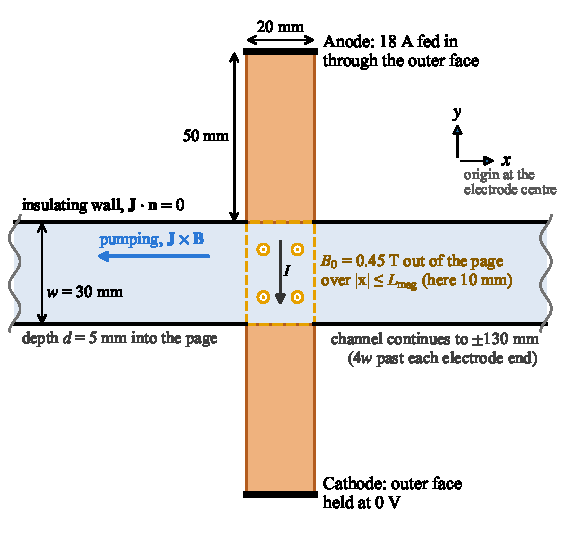
\includegraphics[width=0.6\linewidth]{femm_geometry}
  \caption{Geometry and boundary conditions of the FEMM pump model.}
  \label{fig:femm-geometry}
\end{figure}

\section{Results to Date}

At \SI{18}{\ampere}, the electrode-to-electrode resistance is
\SI{69.6}{\micro\ohm}, and about \SI{40}{\percent} of the current fringes past
the electrode ends, outside the field, where it produces no force
(\cref{fig:femm-jmap}). The model was reduced to a lumped circuit, in which the
Galinstan forms a parasitic path between the electrodes and a fringe path beyond
them, and this circuit reproduced the FEMM force and back-EMF to within
\SI{0.4}{\percent}. From it, the efficiency of the pump has a single peak
(\cref{fig:femm-efficiency}), whose height depends only on the electrode aspect
ratio and the series resistance. \Cref{tab:femm-results} summarises the main
design results.

\begin{figure}[htbp]
  \centering
  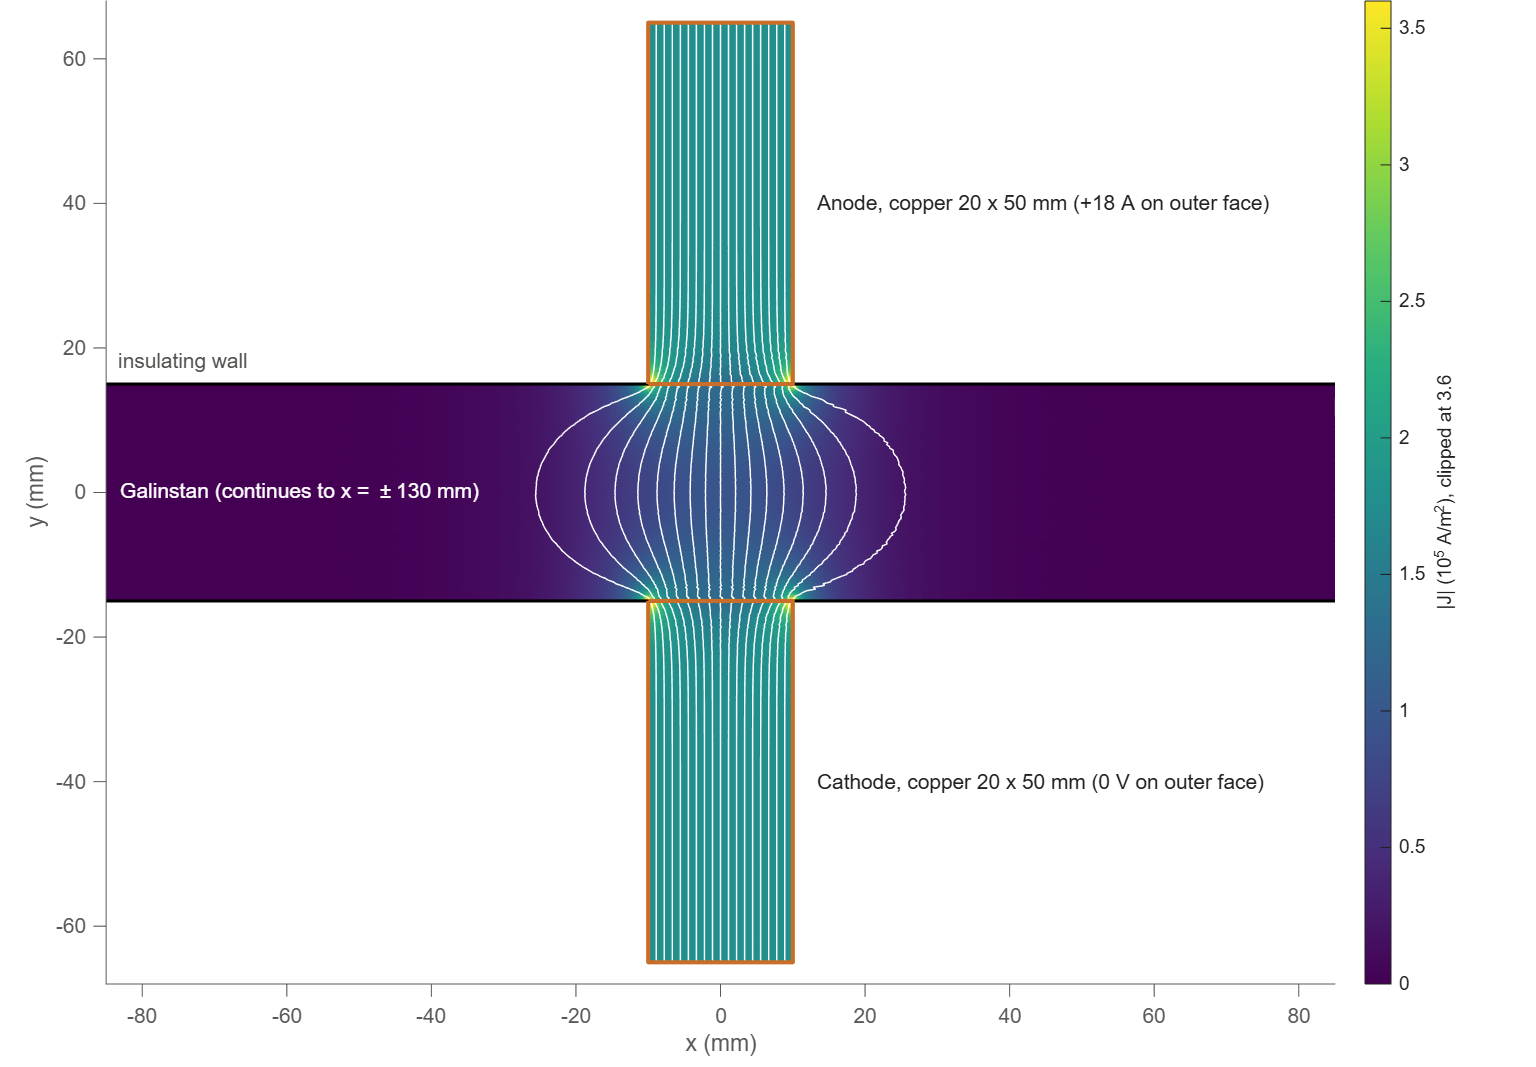
\includegraphics[width=0.6\linewidth]{femm_J_map}
  \caption{Current density in the pump channel at \SI{18}{\ampere}, no flow.}
  \label{fig:femm-jmap}
  \floatnote{Streamlines \SI{1}{\ampere} apart.}
\end{figure}

\begin{figure}[htbp]
  \centering
  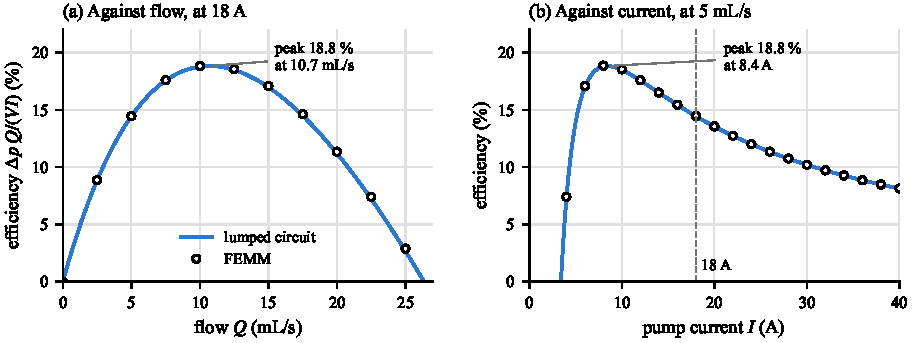
\includegraphics[width=\linewidth]{femm_efficiency}
  \caption{Modelled pump efficiency against flow and current.}
  \label{fig:femm-efficiency}
  \floatnote{\SI{20}{\milli\metre} electrodes, \SI{0.45}{\tesla}; terminal
    efficiency, excluding leads and contacts.}
\end{figure}

\begin{table}[htbp]
  \centering
  \caption{Main results of the FEMM pump model.}
  \label{tab:femm-results}
  \small
  \begin{tabular}{@{}lc@{}}
    \toprule
    Quantity & Value \\
    \midrule
    Electrode-to-electrode resistance & \SI{69.6}{\micro\ohm} \\
    Current inside the field & \SI{60}{\percent} \\
    Zero-flow pressure rise at \SI{18}{\ampere} & \SI{0.98}{\kilo\pascal} \\
    Efficiency at \SI{5}{\milli\litre\per\second}, \SI{18}{\ampere} & \SI{14.5}{\percent} \\
    Peak efficiency, \SI{20}{\milli\metre} electrodes & \SI{18.8}{\percent} \\
    Peak efficiency, \SI{60}{\milli\metre} electrodes & \SI{36.9}{\percent} \\
    Peak efficiency, \SI{20}{\milli\metre} electrodes,
      \SI{50}{\micro\ohm} series resistance & \SI{12.7}{\percent} \\
    \bottomrule
  \end{tabular}
  \floatnote{Terminal efficiency $\Delta p\,Q/(VI)$; the field covers the
    electrodes.}
\end{table}

The design studies suggest three ways to improve the pump. Lengthening the
electrodes, with the field lengthened to match, brings more of the current into
the field and roughly doubles the peak efficiency at \SI{60}{\milli\metre}.
Widening the channel adds flow area but not pressure unless the field is
lengthened with it. A shallower channel gives more pressure per ampere, but at
the cost of higher viscous loss.

The model also points to a likely cause of the low measured efficiency. The
measured pump power of \SI{0.85}{\watt} at \SI{18}{\ampere} corresponds to a
terminal resistance of about \SI{2.6}{\milli\ohm}, nearly 40 times the
\SI{69.6}{\micro\ohm} of the modelled channel and electrodes. Most of the input
power is therefore likely dissipated in the leads, joints and
electrode--Galinstan contacts, which the model does not include. Because the
pump itself is only tens of microohms, even \SI{50}{\micro\ohm} of series
resistance reduces its peak efficiency by about a third
(\cref{tab:femm-results}), so the supply should sit next to the pump on short,
heavy busbars.

\section{Work Remaining}

The model is two-dimensional, so the top and bottom walls, Hartmann layers and
the real velocity profile are not captured, and it assumes a uniform field with
sharp edges, nominal room-temperature conductivities and ideal contacts. To be
used for design, it would need to be validated against measurements of the
pump's pressure--flow curve and terminal voltage, extended to include the
contact and lead resistances and the fringing of the magnet field, and coupled
to the pressure drop of the cooling loop to find the operating point.


\end{document}
